%% LyX 2.3.0 created this file.  For more info, see http://www.lyx.org/.
%% Do not edit unless you really know what you are doing.
\documentclass[english,11pt]{article}

\usepackage[english]{babel} 
\usepackage{amsthm} 


\usepackage{algorithm}
\usepackage{algorithmic}
\usepackage{amssymb}
\usepackage{graphicx}
\usepackage{wrapfig}
% \usepackage{mathtools}
\usepackage{blkarray, bigstrut}
%\usepackage{times}
\usepackage{bm}
\usepackage{ stmaryrd } 

\usepackage{romannum}

\usepackage[normalem]{ulem}
% For derivation rules
\usepackage{mathpartir}
\usepackage{color}
% \usepackage{a4wide}
\usepackage{subcaption} %% For complex figures with subfigures/subcaptions
                        %% http://ctan.org/pkg/subcaption
\usepackage{mathtools}
\DeclarePairedDelimiter{\ceil}{\lceil}{\rceil}
\DeclarePairedDelimiter{\floor}{\lfloor}{\rfloor}
\usepackage{fourier} 
\usepackage{tikz}
\usetikzlibrary{shapes,arrows,snakes,decorations.markings}
\usetikzlibrary{svg.path,arrows.meta, calc} 

\tikzstyle{decision} = [diamond, draw, fill=blue!20, 
    text width=4.5em, text badly centered, node distance=3cm, inner sep=0pt]
% \tikzstyle{block} = [rectangle, draw, fill=blue!20, 
%     text width=5em, text centered, rounded corners, minimum height=4em]
\tikzstyle{block} = [draw, very thick, fill=white, rectangle, 
    minimum height=2.5em, minimum width=6em, text centered]

\tikzstyle{line} = [draw, -latex']
\tikzstyle{cloud} = [draw, ellipse,fill=red!20, node distance=3cm,    minimum height=2em]

\tikzstyle{vecArrow} = [thick, decoration={markings,mark=at position
   1 with {\arrow[semithick]{open triangle 60}}},
   double distance=1.4pt, shorten >= 5.5pt,
   preaction = {decorate},
   postaction = {draw,line width=1.4pt, white,shorten >= 4.5pt}]
\tikzstyle{innerWhite} = [semithick, white,line width=1.4pt, shorten >= 4.5pt]

\usepackage{multirow}


%%%%%%%%%%%%%%%%%%%%%%%%%%%%%%%%%%%%%%%%%%%%%%%%%%%%%Packages And Definitions For Listing the Code%%%%%%%%%%%%%%%%%%%%%%%%%%%%%%%%%%%%%%%%%%%%%%%%%%%%%%%%%%%%%%%%%%%%%%%%
\usepackage{listings}
\usepackage{xcolor}
\usepackage{courier}
\definecolor{codegreen}{rgb}{0,0.6,0}
\definecolor{codegray}{rgb}{0.5,0.5,0.5}
\definecolor{codepurple}{rgb}{0.58,0,0.82}
\definecolor{backcolour}{rgb}{0.95,0.95,0.92}

\lstdefinestyle{mystyle}{
    backgroundcolor=\color{backcolour},   
    commentstyle=\color{codegreen},
    keywordstyle=\color{magenta},
    numberstyle=\tiny\color{codegray},
    stringstyle=\color{codepurple},
    basicstyle=\footnotesize\ttfamily,
    breakatwhitespace=false,         
    breaklines=true,                 
    captionpos=b,                    
    keepspaces=true,                 
    numbers=left,                    
    numbersep=2pt,                  
    showspaces=false,                
    showstringspaces=false,
    showtabs=false,                  
    tabsize=2
}

\lstset{style=mystyle}


%%%%%%%%%%


\include{ldefs}
\newcommand{\THESYSTEM}{\textsf{AdaptFun}}

%%%%%%%%%%%%%%%%%%%%%%%%%%%%%%%%%%%%%%%%%%%%
\makeatletter

\makeatother

\usepackage{babel}
\begin{document}

\title{{\em Dissertation Prospectus}
\\  A Full-Spectrum Dependently Typed
Language for Testing with Dynamic Equality}

\author{Jiawen Liu\\ Department of Computer Science, Boston University \\ \today}
\maketitle
\begin{abstract}
Data analyses are usually designed to identify some property of the population from which the data are drawn, generalizing beyond the specific data sample. For this reason, data analyses are often designed in a way that guarantees that they produce a low generalization error.
   That is, they are designed so that the result of a data analysis run on a sample data does not differ too much from the result one would achieve by running the analysis over the entire population. 
   
   An adaptive data analysis can be seen as a process composed by multiple queries interrogating some data, where the choice of which query to run next may rely on the results of previous queries. 
   The generalization error of each individual query/analysis can be controlled by using an array of well-established statistical techniques.
   However, when queries are arbitrarily composed, the different errors can propagate through the chain of different queries and bring to high generalization error. 
   To address this issue, data analysts are designing several techniques that not only guarantee bounds on the generalization errors of single queries, but that also guarantee bounds on the generalization error of the composed analyses. 
   The choice of which of these techniques to use, 
   often depends on the chain of queries that an adaptive data analysis can generate.
   Specifically the total number of queries and the depth of the chain of queries is of great significance 
   to guarantee the generalization error, 
   when the composed data analyses are adaptive. 
   So in order to give a precise guarantee of generalization error
   for the program,
    I'm interested in analysing depth of the chain of queries in program, i.e., the program's \emph{adaptivity} property.
   % Gap
   % Unfortunately, this depth which relies on the program(implementation) itself is costly in human efforts, and how to statically obtain this information is not well studied to support data analysts.

   In this proposal, I firstly focus on analyse this intuitive \emph{adaptivity} property for the adaptive data analysis programs. 
   Then I propose extensions of this analysis with improved techniques, 
   and a more accurate program's resource cost analysis through
   generalization of this analysis framework, and a reduction from CFL-reachability problem into my analysis framework.
   %  onto general program's resource cost analysis,
   % .
   \\
   Firstly I will analyse this \emph{adaptivity} property for the adaptive data analysis programs in a while-like language.
   Through two aspects: the execution-based analysis and static-based program analysis.
	In the execution-based analysis, I will formalize the intuitive notion of \emph{adaptivity} as a quantitative 
   property of programs. This analysis is developed in three steps through different methodologies in each step. 
   \\
	a. The dependency relation between every query, through the methodology of semantic data dependency analysis.
   \\
	b. The dependency quantity analysis, through the methodology of execution-based data reachability bound analysis.
   \\
	c. The adaptivity analysis, based on the two analysis results above, give the formal \emph{adaptivity} model 
   for program.
   \\   
   % I will focus on research on how to define the Adaptivity semantically. 
   % (the Trace, Event, the Dependency relation, Dependency depth in terms of the evaluation times and the Adaptivity)
	In the static-based program analysis, I will design a static program analysis for soundly approximating this quantity.
   In this static program analysis, the program will be analysed in the same 3 aspects as the execution-based analysis 
   while through static program analysis techniques, and a sound estimated result will be given in each aspect as follows.
   \\
	a. The data dependency relation analysis through the static data flow analysis technique.
   \\
	b. The dependency quantity analysis through the static program reachability bound analysis techniques.
   \\
	c. The program adaptivity estimation, through newly designed algorithms based on the results estimated above, 
   computing the adaptivity upper bound soundly 
   and accurately.
   \\
   I will implement my program analysis and show that it can help to analyse the adaptivity of several concrete data analyses with different adaptivity structures.

   Then, based on the implementation and experimental results, 
   I will focus on improve three features of this full-spectrum analysis.
   \\
   1. I will improve the precision of the \emph{adaptivity} in the formalized model through the execution-based program analysis.
   \\
   2. In static program analysis, I will give tighter estimated upper bound on dependency quantity through 
   path sensitive reachability bound analysis techniques. 
   \\
   3. In the third step of static program analysis, I will improve the accuracy of the adaptivity computation algorithm,
   compute a tighter adaptivity upper bound as well.
   
   Then, through two observations,
   that 
   firstly, traditional program's resource cost analysis they failed to consider the case where the program's cost could decrease 
   implicitly, and 
   % when there isn't a dependency relation between variables.
   the resource consumption during the program 
   execution increases and particularly decreases implicitly in the same way as the program's adaptivity, 
   % Specifically, in line 5 
   % where the list is re-written and the heap consumption is decreased implicitly. 
   % This implicit decrease 
   % of the cost works exactly the same as program's adaptivity decrease.
   I'm interested in improving the accuracy of program's general resource cost analysis
   by generalizing my \emph{adaptivity} analysis framework.
   %  onto the program's resource cost analysis. 
   % Use this framework,
   Through the generalized \emph{adaptivity} analysis framework.
   I will give
   a more accurate resource cost estimation by taking the program's implicit resource cost into consideration, comparing 
   to the worst case cost analysis in traditional way.

   Finally, based on the study on traditional way of performing data flow and control analysis,
   I identify the similarity between the traditional way of performing data flow and control analysis, and the 
   adaptivity analysis.  
   Specifically I identify the similarity between 
   solving the feasible path problem in the analysis by reducing to CFL-reachability problems,
   and the way of computing the adaptivity in my static analysis framework.
   Motivated by this observation, 
   % I'm insterested
   % the, There are similarity between
   % solving the data flow problem by reducing to CFL-reachability problem,
   % resource analysis through reducing to CFL-reachability problem, 
   I'm interested in showing that
   CFL-reachability problems can be solved by reducing it into my adaptivity analysis framework.

  
\end{abstract}
\tableofcontents{}

\section{Introduction to Adaptivity Analysis}
\label{sec:introduction}
% % %%%% Benefit of reasoning about 
% \subsection{Motivation of Reasoning about Adaptivity}
% % 
In Section~\ref{sec:intro-background},
I introduce the background and limitation of the 
adaptive data analysis, 
and the motivation of reasoning about the \emph{adaptivity} quantity property 
for adaptive data analysis.
%  in Section~\ref{sec:intro-motivation}.
% analyzing 
In order to analyze this quantity property for the adaptive data analysis, there are 3 challenges
% problems encountered.
introduced.
% I introduce these three problems
% and the full-spectrum analysis methodologies developed according to these problems 
Targeting to the three challenges, I introduce the methodologies 
of the program analysis framework for the adaptive data analysis's adaptivity property
accordingly, in Section~\ref{sec:intro-adapt}.
Concretely, 
% the full-spectrum 
this analysis framework is developed through the language formalization,
the execution-based analysis, and the static-based program analysis.
%
Based on the implementation and experimental results on this analysis framework, 
I propose three significant 
further features can be improved 
% in the analysis methodologies 
in Section~\ref{sec:intro-improve}, 
and plan to finish these improvements 
before the final defense.
%
 % Next, based on the implementation and experimental results, I proposed two significant 
 % further features can be improved for my analysis framework, and plan to finish the improvement 
 % before the final defense.
 %
 Then, in Section~\ref{sec:intro-cost}, through two observations, 
 I introduce the motivations and methodologies
 for 
%  the accurate 
analyzing program's \emph{non-monotonic} quantitative property accurately.
%   with implicit cost decreases.
% \\
% 1. traditional program's resource cost analysis failed to consider the case where the program's cost could decrease 
% implicitly, 
% \\
% 2. and 
% % when there isn't a dependency relation between variables.
% the resource consumption during the program 
% execution increases and particularly decreases implicitly in the same way as the program's adaptivity, 
% % Specifically, in line 5 
% % where the list is re-written and the heap consumption is decreased implicitly. 
% % This implicit decrease 
% % of the cost works the same as the program's adaptivity decreases.
% I am interested in improving the accuracy of the program's general resource cost analysis
% by 
% % onto the program's resource cost analysis. 
% % Use this framework,
% Through the generalized \emph{adaptivity} analysis framework.
% I will give
% a more accurate resource cost estimation by taking the program's implicit resource cost into consideration, comparing 
% to the worst case cost analysis in a traditional way.

\subsection{Background and Motivation\todo{Rewrite into Program Analysis of the Quantitative Property}}
 \label{sec:intro-background}
 Skeleton:
Usefulness of the Program Analysis on Quantitative Property in different areas.
\\
In Machine Learning Area, the Adaptivity Quantity is significant
==> Major Work I
\\
In Resource Cost Analysis Area, the Reachability-Bound is significant.
==> Major Work II
Technique Limitation:
\\
Path-Sensitive Reachability-Bound 
\\
In Resource Cost Analysis Area, the Reachability-Bound is significant.


\subsection{Proposal Outline}
\label{sec:intro-outline}
\paragraph{Automated Program Analysis Framework for Adaptive Data Analysis (In Improvements)}
\label{sec:intro-adapt}
Based on the implementation and experimental results of the program analysis framework,
%  on the $\THESYSTEM$,
I plan to focus on the following three further features which can be extended and improved.
%  in my full-spectrum analysis.
\begin{enumerate}
    \item In the adaptive data analysis formalization, I plan to extend the {\tt Query While} Language with inter-procedure call.
    \item In the execution-based \emph{adaptivity},
    I plan to improve the precision of the \emph{adaptivity} formalization w.r.t. the program's intuitive adaptivity rounds,
%  in the formal  model 
and extend this analysis with inter-procedure call.
\item In static \emph{adaptivity} analysis, I plan to give a tighter estimated upper bound on \emph{adaptivity}.
%  give a tighter estimated upper bound 
Specifically, I will focus on improving the accuracy of the static \emph{dependency quantity} analysis in the second step through 
developing a new path sensitive reachability bound analysis technique. 
% \item In the third step of static program analysis, I will improve the accuracy of the adaptivity computation algorithm,
% compute a tighter adaptivity upper bound as well.
\end{enumerate}
\paragraph{Path-Sensitive Reachability-Bound Analysis (In Preparation)}
\label{sec:intro-reachability}

\paragraph{Towards Accurate Program Non-Monotonic Quantitative Property Analysis (In Preparation)}
\label{sec:intro-cost}
Moving towards the area of program's quantitative property analysis,
% Then, motivated by the two following aspects, 
there are two interesting observations as follows.
% I am interested 
These two observations motivated me in 
% improving the accuracy of the program's general resource cost analysis
improving the accuracy of the program's general resource cost analysis
by generalizing this \emph{adaptivity} analysis framework.
\begin{itemize}
 \item 
%  In the traditional program's resource cost and quantitative property analysis,
 There are two research areas in the traditional program's resource cost and quantitative property analysis.
%  of program cost analysis, 
One area is type-system based and the other is data-flow/control-flow analysis based. 
In the type-system design-based areas (\cite{GustafssonEL05}, \cite{hoffmann_jost_2022}), 
the analysis technique requires explicit abstraction or data structure de-allocation in order to save or reduce the cost.
 The
 works in both of these two areas fail to recognize the case where program resource consumption or quantitative properties 
 are decreased implicitly or increased \emph{non-monotonically}.
 \item This kind of resource consumption or quantitative properties during the program 
 execution increase and particularly decrease implicitly in the same way as the program's adaptivity. 
 This is explained in detail through an example in Section~\ref*{sec:generalization}.
\end{itemize}
 Based on the observations above, 
 I plan to develop
 an accurate program \emph{non-monotonic} quantitative property analysis framework through generalizing 
 my \emph{adaptivity} analysis framework.
 This framework can give more accurate cost bound than traditional worst-case resource cost estimation methods,
 by taking the program's implicit resource cost decreasing into consideration.
%  compared 
%  to the worst-case cost analysis in the traditional way.

\paragraph*{Proposal Structure}
To sum up, this proposal covers the following topic in each following section.
\begin{enumerate}
\item A while-like language extended with query request feature, named {\tt Query While} Language, 
used to implement 
the adaptive data analysis in Section~\ref{sec:language}.
\item A formal adaptivity model through execution-based adaptivity analysis in Section~\ref{sec:dynamic}.
\item A static program analysis algorithm named {\THESYSTEM} in Section~\ref{sec:static}.
\item Three proposed further features to be improved for the adaptivity analysis framework,
% based on the 
% % formal adaptivity model and {\THESYSTEM}, 
%  full-spectrum 
in Section~\ref{sec:furthers}.
%  presented in Section~\ref{sec:language},~\ref{sec:dynamic} and~\ref{sec:static},
 This proposed work is planned to be done before the final defense.
\item A proposed accurate program resource cost analysis framework generalized from {\THESYSTEM} in Section~\ref{sec:generalization}. 
The analysis framework design is expected to be done with the implementation start off before the final defense.
% \item A proposed plan for solving the CFL-reachability problem via reduction into the {\THESYSTEM} framework in Section~\ref{sec:cfl_reduction},
% expected to start before final defense and developing further after.
\end{enumerate}
\cleardoublepage



\section{The Query Language for Adaptive Data Analysis Program}
\label{sec:language}
In this chapter, we formally introduce the language we will focus on for writing data analyses.  
This is a simple loop language with some primitives for calling queries. 
After defining the syntax of the language and showing an example, we will define its trace-based operational semantics. 
This is the main technical ingredient we will use to define the program's adaptivity.

\section{Syntax of Query While Language}
\label{sec:language-syntax}
The syntax is shown as follows,
\[
\begin{array}{llll}
\mbox{Arithmetic Operators} 
& \oplus_a & ::= & + ~|~ - ~|~ \times 
%
~|~ \div ~|~ \max ~|~ \min\\  
\mbox{Boolean Operators} 
& \oplus_b & ::= & \lor ~|~ \land
\\
%
\mbox{Relational Operators} 
& \sim & ::= & < ~|~ \leq ~|~ == 
\\  
%
\mbox{Label} 
& l & \in & \mathbb{N} \cup \{\lin, \lex\} 
\\ 
%
\mbox{Arithmetic Expression} 
& \aexpr & ::= & 
n \in \mathbb{N}^{\infty} ~|~ {x} ~|~ \aexpr \oplus_a \aexpr 
 ~|~ \elog \aexpr  ~|~ \esign \aexpr
\\
%
\mbox{Boolean Expression} & \bexpr & ::= & 
%
\etrue ~|~ \efalse  ~|~ \neg \bexpr
 ~|~ \bexpr \oplus_b \bexpr
%
~|~ \aexpr \sim \aexpr 
\\
%
\mbox{Expression} & \expr & ::= & v ~|~ \aexpr ~|~ \bexpr ~|~ [\expr, \dots, \expr]
\\  
%
\mbox{Value} 
& v & ::= & { n ~|~ \etrue ~|~ \efalse ~|~ [] ~|~ [v, \dots, v]}  
\\
%
\mbox{Query Expression} 
& {\qexpr} & ::= 
& { \qval ~|~ \aexpr ~|~ \qexpr \oplus_a \qexpr ~|~ \chi[\aexpr]} 
\\
%
\mbox{Query Value} & \qval & ::= 
& {n ~|~ \chi[n] ~|~ \qval \oplus_a  \qval ~|~ n \oplus_a  \chi[n]
    ~|~ \chi[n] \oplus_a  n}
    \\
\mbox{Labeled Command} 
& {c} & ::= &   [\assign {{x}}{ {\expr}}]^{l} ~|~  [\assign {{x} } {{\query(\qexpr)}}]^{l}
~|~ {\ewhile [ \bexpr ]^{l} \edo {c} }
\\
&&&
~|~ {c};{c}  
~|~ \eif([\bexpr]{}^l , {c}, {c}) 
~|~ [\eskip]^l\\ 
\mbox{Event} 
& \event & ::= & 
    ({x}, l, v, \bullet) ~|~ ({x}, l, v, \qval)  ~~~~~~~~~~~ \mbox{Assignment Event} \\
&&& ~|~(\bexpr, l, v, \bullet)   ~~~~~~~~~~~~~~~~~~~~~~~~~~~~~~~~~~ \mbox{Testing Event}
\\
\end{array}
\]
We use following notations to represent the set of corresponding terms:
\[
\begin{array}{lll}
\mathcal{V} & : & \mbox{Set of Variables}  
\\ 
%
\mathcal{VAL} & : & \mbox{Set of Values} 
\\ 
%
\mathcal{QVAL} & : & \mbox{Set of Query Values} 
\\ 
%
\cdom & : & \mbox{Set of Commands} 
\\ 
%
\eventset  & : & \mbox{Set of Events}  
\\
%
\eventset^{\asn}  & : & \mbox{Set of Assignment Events}  
\\
%
\eventset^{\test}  & : & \mbox{Set of Testing Events}  
\\
%
\ldom  & : & \mbox{Set of Labels}  
\\
%%
\mathcal{VAL}  & : & \mbox{Set of Labeled Variables}  
\\
%%
\dbdom  & : & \mbox{{Set of Databases}} 
\\
%
{\mathcal{T}} & : & \mbox{Set of Traces}
\\
%
\qdom & : & \mbox{{Domain of Query Results}}\\
\end{array}
\]
%
Expressions include
standard arithmetic (with value $n \in \mathbb{N}^{\infty}$) and boolean expression, ($\aexpr$ and $\bexpr$) and extended query expressions $\qexpr$.
A query expression $\qexpr$ can be either a simple arithmetic expression $a$, an expression of the form $\chi[\aexpr]$ where $\chi$ represents a row of the database  and  $\aexpr$ represents an index used to identify a specific attribute of the row $\chi$, a combination of two query expressions, $\qexpr \oplus_{a} \qexpr$, or a normal form $\qval$.
For example, the query expression $\chi[3] + 5$  denotes the computation that
obtains
the value in the $3$rd column of $\chi$ in one row and then add $5$ to it.
\\
%
\paragraph{Standard Expression}
The expressions are either the standard one or the extended one.
A standard expression is
% can be 
either a standard arithmetic expression or a boolean expression, or a list of expressions.
An arithmetic expression can be a constant $n$ denoting integer, a variable $x$ from some countable set $\mathcal{VAR}$, binary operation $\oplus_a$ such as addition, product, subtraction, etc, over arithmetic expressions, and also log and sign operation. 
%
A boolean expression can be either {\tt true} or {\tt false}, basic boolean connectives such as logical negation, logical and and or denoted by $\oplus_b$, and basic comparison $sym$ between arithmetic expressions, e.g., $\leq,=,<,$ etc.
Additionally, I also introduce list in expression.
Our language supports primitives for queries, 
where a specific query is specified by a query expression $\qexpr$. 
A query expression contains the necessary information for a query request, for example, 
$\chi[\aexpr]$ represents the values at a certain index $\aexpr$ in a row $\chi$ of the database. 
Query expressions combine access to the database with other expressions, 
for example, $\chi[3] + 5$ represents a query which asks the value from the column 3 of each database raw $\chi$, adds 5 to each of these values, 
and then computes the average of these values.
\paragraph{Query Expression}
The key extension is
%  language supports 
the primitive for queries, where a specific query is specified by a query expression $\qexpr$. 
A query expression contains the necessary information for a query request, 
for example, $\chi[\qexpr]$ represents the values at a certain index $\qexpr$ in a row $\chi$ of the database. 
When this expression is encapsulated by the symbol $\query$,
 $ \query(\chi[\qexpr]) $ represents a query request computation, this computation will compute the average value at certain index over each row of the database as follows,
 \[
  \query(\chi[\qexpr]) = \frac{1}{n}\sum\limits_{i = 0}^{n}\chi_i[\qexpr]
  \]
For example, the query expression $\chi[3]$  denotes the computation that
obtains
the average value in the $3$rd column of $\chi$.

Query expressions combine access to the database with other expressions, 
for example, 
$\chi[3] + 5$ represents a query that asks the value from column 3 of each database raw $\chi$, 
adds 5 to each of these values, and then computes the average of these values as follows, where $n$ is 
database $\chi$'s number of raw.
%
\[
  \query(\chi[3] + 5) = \frac{1}{n}\sum\limits_{i = 0}^{n}\chi_i[3] + 5
  \]


% %
\paragraph{Labeled Command}
Commands are the typical ones from while languages with an additional command $\assign{x}{\query(\qexpr)}$ 
for query requests which can be used to interrogate the database and compute the linear query corresponding to $\qexpr$.
In this the command, the query expression $\qexpr$ is sent to the database server as a request.
Then the server will compute the average value of $\qexpr$ over each row of the hidden database $\chi$ and return us the result.
For instance, when we execute the command $\assign{x}{\query(\chi[3] + 5)}$,
the server will receive query request in form of $\chi[3] + 5$,
then compute the average value of $\chi[3] + 5$ over each raw of $\chi$, and return the result to us. 
The server is used as external API for computing the results over the hidden database $\chi$.
Each command is annotated with a label $l$, we will use natural numbers as labels and we will use them to record
the location of each command, so that we can uniquely identify them.


 
\paragraph{Labeled Variables}
The labeled variables and assigned variables are set of variables annotated by a label. 
We use  
$\mathcal{LV}$ represents the universe of all the labeled variables and 
$\lvar(c) \in \mathcal{P}(\mathcal{V} \times \mathcal{L}) \subseteq \mathcal{LV}$,
represents the set of labeled variables in program $c$,
defined in Definition~\ref{def:lvar}.
Labeled variables in $c$ is the set of assigned variables.
%
%
\begin{defn}[labelled Variables $\lvar$]
  \label{def:lvar}
  {
  $$
    \lvar(c) \triangleq
    \left\{
    \begin{array}{ll}
        \{{x}^l\}           
        & {c} = [{\assign x e}]^{l} 
        \\
        \{{x}^l\}            
        & {c} = [{\assign x \query(\qexpr)}]^{l} 
        \\
        \lvar(c_1) \cup \lvar(c_2) 
        & {c} = {c_1};{c_2}
        \\
        \lvar(c) \cup \lvar(c_2)
        & {c} =\eif([\bexpr]^{l}, c_1, c_2) 
        \\
        \lvar(c')
        & {c}   = \ewhile ([\bexpr]^{l}, {c}')
  \end{array}
  \right.
  $$
  }
  \end{defn}
  $FV: \expr \to \mathcal{P}(\mathcal{V})$, computes the set of free variables in an expression. To be precise,
  $FV(\aexpr)$, $FV(\bexpr)$ and $FV(\qexpr)$ represent the set of free variables in arithmetic
  expression $\aexpr$, boolean expression $\bexpr$ and query expression $\qexpr$ respectively.
  The free variables
  showing up in $c$, which aren't defined before using, are actually the input variables of this program.
  
% \begin{defn}[Assigned Variables ($\avar : \cdom \to \mathcal{P}(\mathcal{V} \times \mathbb{N})$)]
% \label{def:avar}
% {\footnotesize
% $$ \avar_{c} \triangleq
%   \left\{
%   \begin{array}{ll}
%       \{{x}^l\}                   
%       & {c} = [{\assign x e}]^{l} 
%       \\
%       \{{x}^l\}                   
%       & {c} = [{\assign x \query(\qexpr)}]^{l} 
%       \\
%       \avar_{{c_1}} \cup \avar_{{c_2}}  
%       & {c} = {c_1};{c_2}
%       \\
%       \avar_{{c}} \cup \avar_{{c_2}} 
%       & {c} =\eif([\bexpr]^{l}, c_1, c_2) 
%       \\
%       \avar_{{c}'}
%       & {c}   = \ewhile ([\bexpr]^{l}, {c}')
% \end{array}
% \right.
% $$
% }
% \end{defn}
%

% \begin{defn}[labelled Variables $\lvar$]
% \label{def:lvar}
% {\footnotesize
% $$
%   \lvar_{c} \triangleq
%   \left\{
%   \begin{array}{ll}
%       \{{x}^l\} \cup FV(\expr)^{\lin}                  
%       & {c} = [{\assign x e}]^{l} 
%       \\
%       \{{x}^l\}   \cup FV(\qexpr)^{\lin}                
%       & {c} = [{\assign x \query(\qexpr)}]^{l} 
%       \\
%       \lvar_{{c_1}} \cup \lvar_{{c_2}}  
%       & {c} = {c_1};{c_2}
%       \\
%       \lvar_{{c}} \cup \lvar_{{c_2}} \cup FV(\bexpr)^{\lin}
%       & {c} =\eif([\bexpr]^{l}, c_1, c_2) 
%       \\
%       \lvar_{{c}'} \cup FV(\bexpr)^{\lin}
%       & {c}   = \ewhile ([\bexpr]^{l}, {c}')
% \end{array}
% \right.
% $$
% }
% \end{defn}
%
We also defined the set of query variables for a program $c$,
it is the set of variables set to the result of a query in the program formally in Definition~\ref{def:qvar}.
\begin{defn}[Query Variables ($\qvar: \cdom \to \mathcal{P}(\mathcal{LV})$)] 
  \label{def:qvar}
Given a program $c$, its query variables 
$\qvar(c)$ is the set of variables set to the result of a query in the program.
It is defined as follows:
{\footnotesize
$$
  \qvar(c) \triangleq
  \left\{
  \begin{array}{ll}
      \{\}                  
      & {c} = [{\assign x \expr}]^{l} 
      \\
      \{{x}^l\}                  
      & {c} = [{\assign x \query(\qexpr)}]^{l} 
      \\
      \qvar(c_1) \cup \qvar(c_2)  
      & {c} = {c_1};{c_2}
      \\
      \qvar(c_1) \cup \qvar(c_2) 
      & {c} =\eif([\bexpr]^{l}, c_1, c_2) 
      \\
      \qvar(c')
      & {c}   = \ewhile ([\bexpr]^{l}, {c}')
\end{array}
\right.
$$
}
\end{defn}
%
It is easy to see that a program $c$'s query variables is a subset of 
its labeled variables, $\qvar(c) \subseteq \lvar(c)$.
%
%
Every labeled variable in a program is unique, formally as follows with proof in Appendix~\ref{apdx:lvar_unique}.
\begin{lem}[Uniqueness of the Labeled Variables]
  \label{lem:lvar_unique}
  Given any program $c \in \cdom$ with its label variable set $\lvar(c)$,
  every two labeled variables in this set are different.
  \[
    \forall c \in \cdom, x^i, y^j \in \lvar(c) \sthat i \neq j.
    \]
\end{lem}


\section{Trace-based Operational Semantics}
\label{sec:language-os}
The operational semantics is defined based on the event, trace as well as the 
environment, which are introduced firstly as follows.
\paragraph{Event}
An event tracks useful information about each step of the evaluation, as a quadruple. Its first element is either 
an assigned variable (from an assignment command) or a boolean expression (from the guard of if or while command), follows by 
 the label associated to this event, the value evaluated either from the expression assigned to the variable,
or the boolean expression in the guard.
 The last element stores the query information, which a query value whose default is $\bullet$. I declare event projection operator $\pi_i$ which projects the $i$th element from an event.
%
\[
\begin{array}{llllr}
\mbox{Event} 
& \event & ::= & 
    ({x}, l, v, \bullet) ~|~ ({x}, l, v, \qval)  & \mbox{Assignment Event} \\
& & & 
~|~(\bexpr, l, v, \bullet)   
&
\mbox{Testing Event}
\end{array}
\]
%
The event projection operators $\pi_i$ projects the $i$th element from an event: 
\\
$\pi_i : 
\eventset \to \mathcal{VAR}\cup \mbox{Boolean Expression}  \cup \mathbb{N} \cup \mathcal{VAL} \cup \mathcal{QVAL} $ 
% \wqside{use b for Boolean expression?}
\\
%
Another key definition for this {\tt Query While} language with the query primitives extension is the 
\emph{Equivalence} of Query Expression in Definition~\ref{def:query_equal}.
In order to distinguish if a query's choice is affected by previous values, 
% \jl{
% we need to be able to identify whether two queries are the equivalent or not, so that when we change the result of one query, whether another query is affected. For the equivalence of queries, } 
we need to be able to identify whether two queries are the equivalent or not, so that when we change the result of one query, 
whether another query is affected. 
To define equivalence of queries,
quiet different from the equality between the evaluation results as the regular assignment results, 
we are neither observing the syntactic equivalence between the two query expressions,
nor two results return from the database. 
Instead, we define the equivalence of query expression by quantifying over all values returned from database on a certain form of query value, formally as follows.

\begin{defn}[Equivalence of Query Expression]
%
\label{def:query_equal}
% \mg{Two} \sout{2} 
Two query expressions $\qexpr_1$, $\qexpr_2$ are equivalent, denoted as $\qexpr_1 =_{q} \qexpr_2$, if and only if
$$
 \begin{array}{l} 
   \forall \trace \in \mathcal{T} \sthat \exists \qval_1, \qval_2 \in \mathcal{QVAL} \sthat
    (\config{\trace,  \qexpr_1} \qarrow \qval_1 \land \config{\trace,  \qexpr_2 } \qarrow \qval_2) 
    \\
    \quad \land (\forall D \in \dbdom, r \in D \sthat 
    \exists v \in \mathcal{VAL} \sthat 
          \config{\trace, \qval_1[r/\chi]} \aarrow v \land \config{\trace,  \qval_2[r/\chi] } \aarrow v)  
  \end{array}.
$$
 where $r \in D$ is a record in the database domain $D$. 
 As usual, we will denote by $\qexpr_1 \neq_{q} \qexpr_2$  the negation of the equivalence.
\end{defn}
%
\begin{defn}[Event Equivalence]
  Two events $\event_1, \event_2 \in \eventset$ are equivalent, 
  % denoted as $\event_1 \eventeq \event_2$ 
  denoted as $\event_1 = \event_2$ 
  if and only if:
  \[
  \pi_1(\event_1) = \pi_1(\event_2) 
  \land  
  \pi_2(\event_1) = \pi_2(\event_2) 
  \land
  \pi_{3}(\event_1) = \pi_{3}(\event_2)
  \land 
  \pi_{4}(\event_1) =_q \pi_{4}(\event_2)
  \]
  %
  As usual, we will denote by $\event_1 \neq \event_2$  the negation of the equivalence.
  % As usual, we will denote by $\event_1 \eventneq \event_2$  the negation of the equivalence.
  % When it is clear from the context, we omit the subscript $\kw{e}$ and use 
  % $\event_1 = \event_2$ (and $\event_1 \neq \event_2$) for event equivalent
\end{defn}


\begin{defn}[Events Different up to Value ($\diff$)]
  Two events $\event_1, \event_2 \in \eventset are $ \emph{Different up to Value}, 
  denoted as $\diff(\event_1, \event_2)$ if and only if:
  \[
    \begin{array}{l}
  \pi_1(\event_1) = \pi_1(\event_2) 
  \land  
  \pi_2(\event_1) = \pi_2(\event_2) \\
  \land  
  \big(
    (\pi_3(\event_1) \neq \pi_3(\event_2)
  \land 
  \pi_{4}(\event_1) = \pi_{4}(\event_2) = \bullet )
  % \qquad \qquad 
  \lor 
  (\pi_4(\event_1) \neq \bullet
  \land 
  \pi_4(\event_2) \neq \bullet
  \land 
  \pi_{4}(\event_1) \neq_q \pi_{4}(\event_2)) 
  \big)
  \end{array}
  \]
  \end{defn}
% %
\paragraph{Trace}
A trace $\trace \in \mathcal{T} $ is a list of events, 
collecting the events generated along the program execution. $\mathcal{T} $ represents the set of traces. 
A trace can be regarded as the program history, 
which records all the evaluations for assignment commands and guards in $\eif$ and $\ewhile$ command.
This includes queries asked by the analyst during the execution of the program as well. 
I collect the trace with a trace-based operational semantics based on transitions 
of the form $ \config{c, \trace} \to \config{c', \trace'} $. 
It states that a configuration $\config{c, \trace}$,
which consists of a command $c$ to be evaluated and a starting trace $\trace$, 
evaluates to another configuration with the trace updated along with the evaluation of the command $c$ to the normal form of the command $\eskip$.
%
\[
\begin{array}{llll}
\mbox{Trace} & \trace
& ::= & [] ~|~ \trace :: \event
\end{array}
\]
There are some useful operators: the trace concatenation operator $\tracecat: \mathcal{T} \to \mathcal{T} \to \mathcal{T}$, combines two traces.
% I also have the operator $\tlabel : \mathcal{T} \to \ldom$, which gives the set of labels in every event belonging to a trace. 
% The full definitions of these above operators can be found in the appendix.
\begin{defn}[Trace Concatenation, $\tracecat: \mathcal{T} \to \mathcal{T} \to \mathcal{T}$]
  Given two traces $\trace_1, \trace_2 \in \mathcal{T}$, the trace concatenation operator 
  $\tracecat$ is defined as:
  \[
    \trace_1 \tracecat \trace_2 \triangleq
    \left\{
    \begin{array}{ll} 
       \trace_1 & \trace_2 = [] \\
       (\trace_1  \tracecat \trace_2')  :: \event & \trace_2 = \trace_2' :: \event
    \end{array}
    \right.
  \]
  \end{defn}
  %
  % \todo{ need to consider the occurrence times }
  % \\
  % \mg{This definition is not well given. You use a different operator to define it t[:e] which you say it is a shorthand. It cannot be a shorthand because it is used in the definition. I think you need to define two operations, either in sequence or mutually recursive.}
  % \jl{I moved this definition from the main paper into the appendix \ref{apdx:flowsto_event_soundness}. Because this operator is only being used in the soundness proof. And I also feel it doesn't worth to spend many lines in the main paper for defining this complex notation.}
  % Subtrace: $[ : ] : \mathcal{{T} \to \eventset \to \eventset \to \mathcal{T}}$ 
  % \wqside{Confusing, I can not understand the subtraction, it takes a trace, and two events, and this operator is used to subtract these two events?}
  % \[
  %   \trace[\event_1 : \event_2] \triangleq
  %   \left\{
  %   \begin{array}{ll} 
  %   \trace'[\event_1: \event_2]             & \trace = \event :: \trace' \land \event \eventneq \event_1 \\
  %   \event_1 :: \trace'[:\event_2]  & \trace = \event :: \trace' \land \event \eventeq \event_1 \\
  %   {[]} & \trace = [] \\
  %   \end{array}
  %   \right.
  % \]
  % For any trace $\trace$ and two events $\event_1, \event_2 \in \eventset$,
  % $\trace[\event_1 : \event_2]$ takes the subtrace of $\trace$ starting with $\event_1$ and ending with $\event_2$ including $\event_1$ and $\event_2$.
  % \\
  % We use $\trace[:\event_2] $ as the shorthand of subtrace starting from head and ending with $\event_2$, and similary for $\trace[\event_1:]$.
  % \[
  %   \trace[:\event] \triangleq
  %   \left\{
  %   \begin{array}{ll} 
  %  \event' :: \trace'[: \event]             & \trace = \event' :: \trace' \land \event' \eventneq \event \\
  %   \event'  & \trace = \event' :: \trace' \land \event' \eventeq \event \\
  %   {[]}  & \trace = [] 
  %   \end{array}
  %   \right.
  % % \]
  % % \[
  %   \quad
  %   \trace[\event: ] \triangleq
  %   \left\{
  %   \begin{array}{ll} 
  %   \trace'[\event: ]     & \trace =  \event' :: \trace' \land \event \eventneq \event' \\
  %   \event' :: \trace'  & \trace = \event' :: \trace' \land \event \eventeq \event' \\
  %   {[ ] } & \trace = []
  %   \end{array}
  %   \right.
  % \]
  % %
  % \mg{why in the next definition you use ( ) while in the previous ones you didn't? They seem like the same cases. And why you use o.w. instead of []?}
  % An event $\event \in \eventset$ belongs to a trace $\trace$, i.e., $\event \eventin \trace$ are defined as follows:
  % %
  % \begin{equation}
  %   \event \eventin \trace  
  %   \triangleq \left\{
  %   \begin{array}{ll} 
  %     \etrue                  & \trace =  (\event' :: \trace') \land (\event \eventeq \event')
  %                               \\
  %     \event \eventin \trace' & \trace =  (\event' :: \trace') \land (\event \eventneq \event') \\ 
  %     \efalse                 & o.w.
  %   \end{array}
  %   \right.
  % \end{equation}
The belongs to operator $\in : \eventset \to \mathcal{T} \to \{\etrue, \efalse \} $ and its opposite $\not\in$
express whether an event belongs to a trace, formally as follows in Definition~\ref{def:event_belong}.
\begin{defn}[An Event Belongs to A Trace]
  \label{def:event_belong}
    An event $\event \in \eventset$ belongs to a trace $\trace$, i.e., $\event \in \trace$ are defined as follows:
  %
  \begin{equation}
    \event \in \trace  
    \triangleq \left\{
    \begin{array}{ll} 
      \etrue                  & \trace =  \trace' :: \event'
       \land \event = \event'
                                \\
      \event \in \trace' & \trace =  \trace' :: \event'
      \land \event \neq \event' \\ 
      \efalse                 & \trace = []
    \end{array}
    \right.
  \end{equation}
  As usual, we denote by $\event \notin \trace$ that the event $\event$ doesn't belong to the trace $\trace$.
  \end{defn}
  %
  % An event $\event \in \eventset$ belongs to a trace $\trace$ up to value, 
  % i.e., $\event \sigin \trace$ are defined as follows:
  %   %
  % \begin{equation}
  %   \event \sigin \trace  
  %   \triangleq \left\{
  %   \begin{array}{ll} 
  %     \etrue                  & \trace =  (\trace' \tracecate \event')                          \land \pi_1(\event_1) = \pi_1(\event_2) 
  %                               \land  \pi_2(\event_1) = \pi_2(\event_2)  
  %                               % \land \vcounter(\trace \event) = \vcounter()
  %                               \\
  %     \event \sigin \trace'   & \trace =  (\trace' \tracecate \event') 
  %                               \land 
  %                               (\pi_1(\event_1) \neq \pi_1(\event_2) 
  %                               \lor  \pi_2(\event_1) \neq \pi_2(\event_2)) 
  %                               \\ 
  %     \efalse                 & o.w.
  %   \end{array}
  %   \right.
  % \end{equation}
  %
  % % \mg{Why the previous definition used :: and now you switch to ++? Cannot this just be defined using ::? I am trying to anticipate places where a reader might be confused. Also, this definition would be much simpler if we defined event in a more uniform way. Ideally, we want to distinguish three cases, we don't need to distinguish 7 cases.}\\
  % % \jl{My bad, I was really too sticky to the convention.
  % I though the list appending  $::$ can only append element on the left side.}
  % \mg{We introduce a counting operator $\vcounter : \mathcal{T} \to \mathbb{N} \to \mathbb{N}$ whose behavior is defined as follows, \sout{Counter $\vcounter : \mathcal{T} \to \mathbb{N} \to \mathbb{N}$ }}.
  % \wq{The operator counter actually provides the number of times a specific label appears in a trace. Only a number, the position of label is ignored.}
  % \[
  % \begin{array}{lll}
  % \vcounter((x, l, v) :: \trace ) l \triangleq \vcounter(\trace) l + 1
  % &
  % \vcounter((b, l, v):: \trace ) l \triangleq \vcounter(\trace) l + 1
  % &
  % \vcounter((x, l, \qval, v):: \trace ) l \triangleq \vcounter(\trace) l + 1
  % \\
  % \vcounter((x, l', v):: \trace ) l \triangleq \vcounter(\trace ) l
  % &
  % \vcounter((b, l', v):: \trace ) l \triangleq \vcounter(\trace ) l
  % &
  % \vcounter((x, l', \qval, v):: \trace ) l \triangleq \vcounter(\trace ) l
  % \\
  % \vcounter({[]}) l \triangleq 0
  % &&
  % \end{array}
  % \]
  % \[
  % \begin{array}{lll}
  % \vcounter(\trace  \tracecat [(x, l, v)] ) l \triangleq \vcounter(\trace) l + 1
  % &
  % \vcounter(\trace  \tracecat [(b, l, v)] ) l \triangleq \vcounter(\trace) l + 1
  % &
  % \vcounter(\trace  \tracecat [(x, l, \qval, v)] ) l \triangleq \vcounter(\trace) l + 1
  % \\
  % \vcounter(\trace  \tracecat [(x, l', v)] ) l \triangleq \vcounter(\trace ) l
  % &
  % \vcounter(\trace  \tracecat [(b, l', v)] ) l \triangleq \vcounter(\trace ) l
  % &
  % \vcounter(\trace  \tracecat [(x, l', \qval, v)]) l \triangleq \vcounter(\trace ) l
  % \\
  % \vcounter({[]}) l \triangleq 0
  % &&
  % \end{array}
  % \]
  We introduce a counting operator $\vcounter : \mathcal{T} \to \mathbb{N} \to \mathbb{N}$ whose behavior is defined as follows,
  % \[
  % \begin{array}{lll}
  % \vcounter(\trace :: (x, l, v, \bullet) ) l \triangleq \vcounter(\trace) l + 1
  % &
  % \vcounter(\trace  ::(b, l, v, \bullet) ) l \triangleq \vcounter(\trace) l + 1
  % &
  % \vcounter(\trace  :: (x, l, v, \qval) ) l \triangleq \vcounter(\trace) l + 1
  % \\
  % \vcounter(\trace  :: (x, l', v, \bullet) ) l \triangleq \vcounter(\trace ) l, l' \neq l
  % &
  % \vcounter(\trace  :: (b, l', v, \bullet) ) l \triangleq \vcounter(\trace ) l, l' \neq l
  % &
  % \vcounter(\trace  :: (x, l', v, \qval)) l \triangleq \vcounter(\trace ) l, l' \neq l
  % \\
  % \vcounter({[]}) l \triangleq 0
  % &&
  % \end{array}
  % \]
  \begin{defn}[Occurrence Counter]
    \[
  \begin{array}{lll}
  \vcounter(\trace :: (x, l, v, \bullet), l ) \triangleq \vcounter(\trace, l) + 1
  &
  \vcounter(\trace  ::(b, l, v, \bullet), l) \triangleq \vcounter(\trace, l) + 1
  &
  \vcounter(\trace  :: (x, l, v, \qval), l) \triangleq \vcounter(\trace, l) + 1
  \\
  \vcounter(\trace  :: (x, l', v, \bullet), l) \triangleq \vcounter(\trace, l), l' \neq l
  &
  \vcounter(\trace  :: (b, l', v, \bullet), l) \triangleq \vcounter(\trace, l), l' \neq l
  &
  \vcounter(\trace  :: (x, l', v, \qval), l) \triangleq \vcounter(\trace, l), l' \neq l
  \\
  \vcounter({[]}, l) \triangleq 0
  &&
  \end{array}
  \]
\end{defn}
Another operator $\llabel : \mathcal{T} \to \mathcal{VAR} \to \{\mathbb{N}\}\cup \{\bot\}$,
takes a trace and a variable as input and returns the label of the latest assignment event which assigns value to that variable. 
  % We introduce an operator $\llabel : \mathcal{T} \to \mathcal{VAR} \to \ldom \cup \{\bot\}$, which 
  % takes a trace and a variable and returns the label of the latest assignment event which assigns value to that variable.
  Its behavior is defined as follows,
  \begin{defn}[Latest Label]
    \[
      % \begin{array}{lll}
    \llabel(\trace  :: (x, l, \_, \_)) x \triangleq l
    ~~~
    \llabel(\trace  :: (y, l, \_, \_)) x \triangleq \llabel(\trace ) x, y \neq x
    % &
    ~~~
    \llabel(\trace :: (b, l, v, \bullet)) x \triangleq \llabel(\trace) x
    % &
    % \\
    % \llabel(\trace  :: (y, l, v, \bullet)) x \triangleq \llabel(\trace ) x
    % &
    % \llabel(\trace :: (y, l, v, \qval)) x \triangleq \llabel(\trace ) x
    % &
    ~~~
    \llabel({[]}) x \triangleq \bot
    % \end{array}
    \]
  \end{defn}
  %
    The operator $\tlabel : \mathcal{T} \to \mathcal{P}{(\ldom)}$ gives the set of labels in every event belonging to 
    a trace, whose behavior is defined as follows,
  \[
    % \begin{array}{llll}
  \tlabel{(\trace  :: (\_, l, \_, \_)])} \triangleq \{l\} \cup \tlabel{(\trace )}
  ~~~
  \tlabel({[ ]}) \triangleq \{\}
  % \end{array}
  \]
  %
  % \mg{The next lemma is trivial but it still needs a proof sketch.}
  If we observe the operational semantics rules, we can find that no rule will shrink the trace. 
  So we have the Lemma~\ref{lem:tracenondec} with proof in Appendix~\ref{apdx:lemma_sec123}, 
  specifically the trace has the property that its length never decreases during the program execution.
  \begin{lem}
  [Trace Non-Decreasing]
  \label{lem:tracenondec}
  For every program $c \in \cdom$ and traces $\trace, \trace' \in \mathcal{T}$, if 
  $\config{c, \trace} \rightarrow^{*} \config{\eskip, \trace'}$,
  then there exists a trace $\trace'' \in \mathcal{T}$ with $\trace \tracecat \trace'' = \trace'$
  %
  $$
  \forall \trace, \trace' \in \mathcal{T}, c \sthat 
  \config{c, \trace} \rightarrow^{*} \config{\eskip, \trace'} 
  \implies \exists \trace'' \in \mathcal{T} \sthat \trace \tracecat \trace'' = \trace'
  $$
  \end{lem}
  Since the equivalence over two events is defined over the query value equivalence, 
  when there is an event belonging to a trace, 
  if this event is a query assignment event, 
  it is possible that 
  the event showing up in this trace has a different form of query value, 
  but they are equivalent by Definition~\ref{def:query_equal}.
  So we have the following Corollary~\ref{coro:aqintrace} with proof in Appendix~\ref{apdx:lemma_sec123}.
  \begin{coro}
  \label{coro:aqintrace}
  For every event and a trace $\trace \in \mathcal{T}$,
  if $\event \in \trace$, 
  then there exist another event $\event' \in \eventset$ and traces $\trace_1, \trace_2 \in \mathcal{T}$
  such that $\trace_1 \tracecat [\event'] \tracecat \trace_2 = \trace $
  with 
  $\event$ and $\event'$ equivalent but may differ in their query value.
  \[
    \forall \event \in \eventset, \trace \in \mathcal{T} \sthat 
  \event \in \trace \implies \exists \trace_1, \trace_2 \in \mathcal{T}, 
  \event' \in \eventset \sthat (\event \in \event') \land \trace_1 \tracecat [\event'] \tracecat \trace_2 = \trace  
  \]
  \end{coro}
%  
\paragraph{Environment}
An environment is standard, a map from variables to values.
$\env : {\mathcal{T}}  \to \mathcal{VAR} \to \mathcal{VAL} \cup \{\bot\}$, 
which maps a trace and a variable to the latest value assigned to this variable on the trace is defined as follows.
Queries can be uniquely annotated as $\mathcal{AQ}$, and the annotation $(l,w)$ considers the location of the query by line number $l$ and which 
iteration the query is at when it appears in a loop statement, specified by $w$. A trace $t$ is a list of annotated queries accumulated along the execution of the program. 

\[
\begin{array}{lll}
\env(\trace  \traceadd (x, l, v, \bullet)) x \triangleq v
&
\env(\trace \traceadd (y, l, v, \bullet)) x \triangleq \env(\trace) x, y \neq x
&
\env(\trace \traceadd (b, l, v, \bullet)) x \triangleq \env(\trace) x
\\
\env(\trace \traceadd (x, l, v, \qval)) x \triangleq v
&
\env(\trace \traceadd (y, l, v, \qval)) x \triangleq \env(\trace) x, y \neq x
&
\env({[]} ) x \triangleq \bot
\end{array}
\]
 %% trace

 \paragraph*{Operational Semantics}
 The complete operational semantic evaluation rules are presented in Figure~\ref{fig:os},
 with the evaluation rules for expressions in Figure~\ref{fig:expr_eval}.

 The rule $\textbf{assn}$ evaluates a standard assignment $\assign{x}{\expr}$, the expression $\expr$ is first evaluated by our expression evaluation $\config{\trace, \expr} \earrow v $, presented below. And the result $v$ of evaluating $\expr$ is used to construct a new event $\event = (x, l, v,\bullet)$ and attach to the previous trace.  
\begin{figure}
\begin{mathpar}
\boxed{ \config{\trace,\aexpr} \aarrow v \, : \, \mbox{Trace  $\times$ Arithmetic Expr $\Rightarrow$ Arithmetic Value} }
\\
% \text{\mg{Missing. Without these rules it is difficult to understand why we need a trace to evaluate expressions.}}
% \\
\inferrule{ 
  \empty
}{
 \config{\trace,  n} 
 \aarrow n
}
\and
\inferrule{ 
  \env(\trace) x = v
}{
 \config{\trace,  x} 
 \aarrow v
}
\and
\inferrule{ 
  \config{\trace, \aexpr_1} \aarrow v_1
  \and 
  \config{\trace, \aexpr_2} \aarrow v_2
  \and 
   v_1 \oplus_a v_2 = v
}{
 \config{\trace,  \aexpr_1 \oplus_a \aexpr_2} 
 \aarrow v
}
\and
\inferrule{ 
  \config{\trace, \aexpr} \aarrow v'
  \and 
  \elog v' = v
}{
 \config{\trace,  \elog \aexpr} 
 \aarrow v
}
\and
\inferrule{ 
  \config{\trace, \aexpr} \aarrow v'
  \and 
  \esign v' = v
}{
 \config{\trace,  \esign \aexpr} 
 \aarrow v
}
\\
\boxed{ \config{\trace, \bexpr} \barrow v \, : \, \mbox{Trace $\times$ Boolean Expr $\Rightarrow$ Boolean Value} }
\\
\inferrule{ 
  \empty
}{
 \config{\trace,  \efalse} 
 \barrow \efalse
}
\and 
\inferrule{ 
  \empty
}{
 \config{\trace,  \etrue} 
 \barrow \etrue
}
\and 
\inferrule{ 
  \config{\trace, \bexpr} \barrow v'
  \and 
  \neg v' = v
}{
 \config{\trace,  \neg \bexpr} 
 \barrow v
}
\and 
\inferrule{ 
  \config{\trace, \bexpr_1} \barrow v_1
  \and 
  \config{\trace, \bexpr_2} \barrow v_2
  \and 
   v_1 \oplus_b v_2 = v
}{
 \config{\trace,  \bexpr_1 \oplus_b \bexpr_2} 
 \barrow v
}
\and 
\inferrule{ 
  \config{\trace, \aexpr_1} \aarrow v_1
  \and 
  \config{\trace, \aexpr_2} \aarrow v_2
  \and 
   v_1 \sim v_2 = v
}{
 \config{\trace,  \aexpr_1 \sim \aexpr_2} 
 \barrow v
}
\\
\boxed{ \config{\trace, \expr} \earrow v \, : \, \mbox{Trace $\times$ Expression $\Rightarrow$ Value} }
\\
\inferrule{ 
  \config{\trace, \aexpr} \aarrow v
}{
 \config{\trace,  \aexpr} 
 \earrow v
}
\and
\inferrule{ 
  \config{\trace, \bexpr} \barrow v
}{
 \config{\trace,  \bexpr} 
 \earrow v
}
\and
\inferrule{ 
  \config{\trace, \expr_1} \earrow v_1
  \cdots
  \config{\trace, \expr_n} \earrow v_n
}{
 \config{\trace,  [\expr_1, \cdots, \expr_n]} 
 \earrow [v_1, \cdots, v_n]
}
\and
\inferrule{ 
  \empty
}{
 \config{\trace,  v} 
 \earrow v
}
\\
\boxed{ \config{\trace, \qexpr} \qarrow \qval \, : \, \mbox{Trace  $\times$ Query Expr $\Rightarrow$ Query Value} }
\\
\inferrule{ 
  \config{\trace, \aexpr} \aarrow n
}{
 \config{\trace,  \aexpr} 
 \qarrow n
}
\and
\inferrule{ 
  \config{\trace, \qexpr_1} \qarrow \qval_1
  \and
  \config{\trace, \qexpr_2} \qarrow \qval_2
}{
 \config{\trace,  \qexpr_1 \oplus_a \qexpr_2} 
 \qarrow \qval_1 \oplus_a \qval_2
}
\and
\inferrule{ 
  \config{\trace, \aexpr} \aarrow n
}{
 \config{\trace, \chi[\aexpr]} \qarrow \chi[n]
}
\and
\inferrule{ 
  \empty
}{
 \config{\trace,  \qval} 
 \qarrow \qval
}
 \end{mathpar}
 \caption{Trace-based Operational Semantics Evaluation Rules for Expression.}
 \label{fig:expr_eval}
\end{figure}

The expression evaluation rules rely on the evaluation of 
arithmetic expressions $\config{\trace,\aexpr} \aarrow v $ 
and boolean expressions $\config{\trace, \bexpr} \barrow v $.

 The step trace-based operational semantics has the form of $ \config{c, \trace} \xrightarrow{} { \config{c', \trace'}}$. 
It reads the configuration $\config{c, \trace}$ consisting of a labeled command $c$ and a pre-trace $\trace$, 
and evaluates it to another configuration, 
in which $c$ is evaluated to $c'$ and trace $\trace$ is updated to $\trace'$. 
\begin{figure}
\begin{mathpar}
\boxed{
\mbox{Command $\times$ Trace}
\xrightarrow{}
\mbox{Command $\times$ Trace}
}
\and
\boxed{\config{{c, \trace}}
\xrightarrow{} 
\config{{c',  \trace'}}
}
\\
\inferrule
{
\empty
}
{
\config{\clabel{\eskip}^l,  \trace } 
\xrightarrow{} 
\config{\clabel{\eskip}^l, \trace}
}
~\textbf{skip}
%
\and
%
\inferrule
{
\event = ({x}, l, v, \bullet)
}
{
\config{[\assign{{x}}{\aexpr}]^{l},  \trace } 
\xrightarrow{} 
\config{\clabel{\eskip}^l, \trace \traceadd \event}
}
~\textbf{assn}
%
\and
%
{
\inferrule
{
 \trace, \qexpr \qarrow \qval
 \and 
\query(\qval) = v
\and 
\event = ({x}, l, v, \qval)
}
{
\config{{[\assign{x}{\query(\qexpr)}]^l, \trace}}
\xrightarrow{} 
\config{{\clabel{\eskip}^l,  \trace \traceadd \event} }
}
~\textbf{query}
}
%
\and
%
\inferrule
{
 \trace, b \barrow \etrue
 \and 
 \event = (b, l, \etrue, \bullet)
}
{
\config{{\ewhile [b]^{l} \edo c, \trace}}
\xrightarrow{} 
\config{{
c; \ewhile [b]^{l} \edo c),
\trace \traceadd \event}}
}
~\textbf{while-t}
%
%
\and
%
\inferrule
{
 \trace, b \barrow \efalse
 \and 
 \event = (b, l, \efalse, \bullet)
}
{
\config{{\ewhile [b]^{l}, \edo c, \trace}}
\xrightarrow{} 
\config{{
  \clabel{\eskip}^l,
\trace \traceadd \event}}
}
~\textbf{while-f}
\and
\inferrule
{
\config{{c_1, \trace}}
\xrightarrow{}
\config{{c_1',  \trace'}}
}
{
\config{{c_1; c_2, \trace}} 
\xrightarrow{} 
\config{{c_1'; c_2, \trace'}}
}
~\textbf{seq1}
%
\and
%
\inferrule
{
  \config{{c_2, \trace}}
  \xrightarrow{}
  \config{{c_2',  \trace'}}
}
{
\config{{\clabel{\eskip}^l; c_2, \trace}} \xrightarrow{} \config{{ c_2', \trace'}}
}
~\textbf{seq2}
%
\and
%
%
\inferrule
{
   \trace, b \barrow \etrue
 \and 
 \event = (b, l, \etrue, \bullet)
}
{
 \config{{
\eif([b]^{l}, c_1, c_2), 
\trace}}
\xrightarrow{} 
\config{{c_1, \trace \traceadd \event}}
}
~\textbf{if-t}
%
\and
%
\inferrule
{
 \trace, b \barrow \efalse
 \and 
 \event = (b, l, \efalse, \bullet)
}
{
\config{{\eif([b]^{l}, c_1, c_2), \trace}}
\xrightarrow{} 
\config{{c_2, \trace \traceadd \event}}
}
~\textbf{if-f}
\end{mathpar}
% \end{subfigure}
    \caption{Trace-based Operational Semantics for Language.}
    \label{fig:os}
\end{figure}

Distinguished from the standard assignment evaluation, 
the rule $\textbf{query}$ 
evaluates a query requesting command $\clabel{\assign{x}{\query(\qexpr)}}^l$ in two steps.
The query expression $\qexpr$ is first evaluated into a query value $\qval$ by following the rules below.
Then, by sending this query request $\query(\qval)$  to a hidden mechanism, this query is evaluated to a result value returned from it, $v = \query(\qval)$.
% by sending this query request $\query(\qval)$  to it.
Also, the generated event stores both the query value $\alpha$ here, and the result value of the query request.

The rules for if and while both have two versions, 
when the boolean expressions in the guards are evaluated to true and false, respectively. 
In these rules, the evaluation of the guard generates a testing event and the trace is updated as well by appending this event.


% \todo{Make sure the operational semantics is big step, and correct assn rules.}
% \jl{


\cleardoublepage

\section{The Program Dynamic Analysis for Adaptivity}
\label{sec:dynamic}

Based on the language and the trace-based operational semantics in Section~\ref{sec:language},
I present an execution-based program adaptivity analysis in this section.
This analysis formalizes the intuitive \emph{adaptivity} through three steps in 
Section~\ref{subsec:dynamic-methodology}.
% ,~\ref{subsubsec:dynamic-reachability}
% % I  an execution based program analysis in this section.
% and~\ref{subsubsec:dynamic-adapt}.
Then through an example in Section~\ref{subsec:dynamic-examples}, I show that the formalized
% can give the 
adaptivity matches the program's intuitive \emph{adaptivity}.

\subsection{Introduction}
\label{subsec:dynamic-intro}

% In order to formalize a quantitative property w.r.t. the dependency relation in the program, I
% use a three-step analysis methodology developed as follows,
% \\
%  a. The dependency relation between every query, through the methodology of semantic data dependency analysis.
% \\
%  b. The dependency quantity analysis, through the methodology of execution-based data reachability bound analysis. Then 
% \\
%  c. The adaptivity analysis, based on the two analysis results above, 
%  I construct an execution-based dependency graph combining the dependency relation and the dependency quantity
%  and give the formal \emph{adaptivity} definition 
%  for program.
% \\
% The construction of this graph requires me to think about the dependency relation between two queries using what we have at hand - 
% the trace generated in Section~\ref{sec:language}. 
 \paragraph*{Related Work}
 {
My framework constructs an execution-based dependency graph based on the execution traces of a program. I define semantic dependence on this graph by considering (intraprocedural) data and control dependency~\cite{bilardi1996framework,cytron1991efficiently,pollock1989incremental}. 
One related work 
\cite{austin1992dynamic} presents a methodology to construct a dynamic dependency graph (DDG) based on the dynamic execution of a program in an imperative language, where edges represent dependency between instructions. Data dependency, control dependency, storage dependency, and resource dependency between instructions are all considered. My execution-based dependency graph only needs data dependency and control dependency between variable assignment results. 
% Critical path length analysis on DDGs is useful for understanding the scope for parallelization, while we use the length of the longest path to define adaptivity. 
%
DDGs have been used in many other domains. \cite{nagar2018automated} use DDGs to find serializability violations. \cite{hammer2006dynamic} use similar \emph{program dependency graphs} \cite{ferrante1987program} for dynamic program slicing.
\cite{mastroeni2008data} propose ways of constructing different kinds of program slices, by choosing different program dependencies. 
% For example, in either syntactic or semantics sense.
% This abstract dependency is based on properties rather than exact data.
% Aims to give finer and smaller program slice. 
They use a combination of 
static and dynamic dependency graphs but in a manner that is different from how we use the two. Their slicing uses both static and dynamic dependency graphs, while we use the dynamic dependency graph as the basis of a definition, which is then soundly approximated by an analysis based on the static dependency graph.}

{My execution-based data dependency relation definition over variables 
is inspired by the method in \cite{Cousot19a}, where the dependency relation is also identified by looking into the differences on two execution traces. 
However, Cousot excludes timing channels~\cite{SabelfeldM03} and empty observation, which are also not considered as a form of dependency in traditional dependency analysis \cite{DenningD77}.
% In the cases of empty observation and timing channels, the second query is executed 
% in one trace and isn't in another trace by modifying the value of the first query. 
% Then, the second query is indeed dependent on the first query and there exists an
% adaptivity round between the two queries. 
My definition includes timing channels and empty observation by observing both the disappearance and value variation.
}
\paragraph*{Execution-Based Adaptivity Analysis Overview}
To formalize this intuition as a quantitative program property, I develop an execution-based analysis
% I first consider all the possible evaluations of a program --- I do this by 
% I use a trace semantics recording the execution history of programs on some given input --- and I create a dependency graph, where the dependency between different variables (query is also assigned to a variable) is explicit and track which variable is associated with a query request. 
% I then enrich this graph with weights describing the maximal number of times each variable is evaluated in a program evaluation starting with an initial state. The adaptivity is then defined as the length of the walk visiting most query-related variables on this graph. 
% Through two aspects: the execution-based analysis and static-based program analysis.
% In the execution-based analysis, I will formalize the intuitive notion of \emph{adaptivity} as a quantitative 
% property of programs. This analysis is developed 
 in three steps as follows,
 \begin{enumerate}
 \item The first step on \emph{dependency relation} analysis is presented in Section~\ref{subsubsec:dynamic-datadep}.
 In this step, I define the variable \emph{may-dependency} relation based on the trace semantics in Section~\ref{sec:language-os}.
%   to analyze the \emph{dependency relation} between every query, 
%  through the methodology of semantic data dependency analysis.
%  %
%  Specifically through a trace semantics recording the execution history of programs on given input,
%  % --- and I create a dependency graph, 
%  the dependency between different variables (query is also assigned to a variable) is explicitly tracked and 
%  analyzed.
%   and 
%   which variable is associated with a query request. 
% I then enrich this graph with weights describing the maximal number of times each variable is evaluated in a program evaluation starting with an initial state. The adaptivity is then defined as the length of the walk visiting most query-related variables on this graph. 
% In the execution-based analysis, I will formalize the intuitive notion of \emph{adaptivity} as a quantitative 
% property of programs. This analysis is developed 
% \\
 \item In the second step in Section~\ref{subsubsec:dynamic-reachability}, I analyze the \emph{dependency quantity} through the methodology of execution-based reachability bound analysis.
%  As 
% %  analysis, 
% based on the \emph{dependency relation} above.
% This analysis is developed through the methodology of execution-based reachability bound analysis.
% \\
 \item The last step is the intuitive \emph{adaptivity} quantity analysis presented in Section~\ref{subsubsec:dynamic-adapt}.
 According to the two analysis results above, specifically \emph{dependency relation} and \emph{dependency quantity},
 I define the formal \emph{adaptivity} model in definition~\ref{def:trace_adapt} through 
 construct a dependency graph.
%  This analysis is developed through the formal \emph{adaptivity} definition. \\
%  Specifically, I create a dependency graph, where the dependency between different variables (query is also assigned to a variable) is explicit and track which variable is associated with a query request. 
%  I then enrich this graph with weights describing the maximal number of times each variable is evaluated in a program evaluation starting with an initial state. 
%  The adaptivity is then defined as the length of the walk visiting most query-related variables on this graph. 
 \end{enumerate}




\subsection{Methodology}
\label{subsec:dynamic-methodology}

\subsubsection{Data Dependency Analysis}
\label{subsubsec:dynamic-datadep}
\paragraph{Challenge}
\label{para:exe-dep-challenge}
In the data analysis model the programming framework supports, 
%  an \emph{analyst} asks a sequence of queries to the mechanism, and receives the answers to these queries from the mechanism. In this model, the adaptivity I are interested in is the length of the longest sequence of such adaptively chosen queries, among all the queries the data analyst asks. 
  I define that a query is adaptively chosen when it is affected by answers of previous queries. The next thing is to decide how do I define whether one query is "affected" by previous answers, with the limited information I have? As a reminder, 
 when the analyst asks a query, the only known information will be the answers to previous queries and the current execution trace of the program.


There are two possible situations that a query will be "affected",  
either when the query expression directly uses the results of previous queries (data dependency), or when the control flow of the program with respect to a query (whether to ask this query or not) depends on the results of previous queries (control flow dependency).
% As a first step, I give a definition of when one query may depend on a previous query, which is supposed to consider both control dependency and data dependency. We first look at two possible candidates:
% \begin{enumerate}
%     \item One query may depend on a previous query if and only if a change of the answer to the previous query may also change the result of the query.
%     \item One query may depend on a previous query if and only if a change of the answer to the previous query may also change the appearance of the query.
% \end{enumerate}


Since the results of previous queries can be stored or used in variables
which aren't associated to the query request,
it is necessary to track the dependency between queries, through all the program's variables.
In the meantime, the trace-based operational semantics tracks the information,
distinguishing variables which are assigned with query requests.
% and then I can distinguish variables which are assigned with query requests.
In this way, the \emph{may-dependency} relation between queries can be recovered through 
the \emph{may-dependency} relation over all the program's variables.
According to this, I focus on the analysis on the variable \emph{may-dependency} relation in the following of this section.

I give a definition of when one variable \emph{may-depend} on a previous variable with two candidates.
{
\begin{enumerate}
    \item One variable may depend on a previous variable if and only if a change of the value assigned to the previous variable may also change the value assigned to the variable.
    \item One variable may depend on a previous variable if and only if a change of the value assigned to the previous variable may also change the appearance of the assignment command to this variable 
    % in\wq{during?} 
    during execution.
\end{enumerate}
}
%   The first candidate works well by witnessing the result of one query according to the change of the answer of another query. We can easily find that the two queries have nothing to do with each other in a simple example   

{   
% The first situations works well by witnessing the result assigned to variable 
% according to the change of the value assigned to another query. 
% We can easily find that the two queries have nothing to do with each other in a simple example 
% In the first one, by defining the dependency as
The first definition is defined as
% witnessing 
% the query expressions equivalence (or the value equality for non-query assignment )
the witness of a variation on the value assigned to the same variable through two executions,
% assigned to the same variable through two executions, 
according to the change of the value assigned to another variable in pre-trace.
% the situation of data-dependency works well. \wq{long sentence, make it short?}
In particular for query requests, the variation I observe is on the query value instead of on the query requesting results.
% We can find that two queries 
% % have nothing to do with each other in this simple example 
% % depends on each other\wq{not each other, one direction.} 
% satisfy this definition
In 
%this 
the simple program $c_1 =\assign{x}{\query(\chi[2])} ;\assign{y}{\query(\chi[3] + x)}$.
 %
 From our perspective, $\query(\chi[1])$ is different from $\query(\chi[2]))$. Informally, I think $\query(\chi[3] + x)$ may depend on the query $\query(\chi[2]))$, because equipped function of the former $\chi[3] + x$ may depend on the data stored in x assigned with the result of $\query(\chi[2]))$, according to this definition. }
%
% in this example: $c_1 = \assign{x}{\query(0)}; \assign{z}{\query(\chi[x])}$.
% This candidate definition works well 
Nevertheless, the first definition fails to catch control dependency because it just monitors the changes to a query, but misses the appearance of the query when the answers of its previous queries change. 
For instance, it fails to handle $
      c_2 = \assign{x}{\query(\chi[1])} ; \eif( x > 2 , \assign{y}{\query(\chi[2])}, \eskip )
   $, but the second definition can. However, it only considers the control dependency and misses the data dependency. 
  This reminds me to define a \emph{may-dependency} relation between labeled variables by combining the two definitions to capture the two situations.
%
%
% I define the According to the trace-based operational semantics,
%
\paragraph*{Value Difference on Traces}
%
\highlight{
  To define the \emph{may-dependency} relation on two labeled variables, I rely on the limited information at hand - the trace generated by the operational semantics. In this end, 
% So I first define some operations on the trace.
% In order to define the \emph{may-dependency} relation, 
Specifically, we need to be able to observe the difference of the values for each variable
through traces, i.e., through the events contained in traces.
Followed by this, it is necessary to give formal definition on observing this difference through traces.
Given the limitation of previous definition based on limited language,
I present the new definitions on observing the value difference as follows.
These new definitions help in formally capturing the intuitive \emph{adaptivity} precisely, concisely, and efficiently.}
%  in order to observe the evaluation variation in a different way, formally as follows.
\highlight{
\begin{defn}[Value Sequence $\seq(\trace, x^l)$]
  \label{def:vseq}
  \[
\begin{array}{l}
  \seq(\trace :: (x, l, v, \bullet), x^l) \triangleq \seq(\trace)::v  \qquad
  \seq(\trace :: (x, l, v, \qval), x^l) \triangleq \seq(\trace):: \qval \qquad
  \seq([]) \triangleq []\\
  \seq(\trace :: (y, j, \_, \_), x^l) \triangleq \seq(\trace) \quad y \neq x \lor j \neq l 
\end{array}
\]
\end{defn}
%
\begin{defn}[Difference Sequence $\sdiff(\trace_1, \trace_2, x^l )$]
  \label{def:diffseq}
  Let $ s_1 = \seq(\trace_1, x^l) \land s_2 = \seq(\trace_2, x^l)$ be the value sequence of $x^l$ 
  on $\trace_1$ and $\trace_2$, and $s^l$ be the sequence with longer length and $s^t$ the 
  shorter one,
  then their difference sequence is defined as follows,
  \[
    \sdiff(\trace_1, \trace_2, x^l) \triangleq
    \begin{array}{l}
      \{ (s^t[k], s^l[k]) ~|~ 
      % \land 
      % \land 
      s^t[k] \neq s^l[k], k = 0, \ldots, len(s^t)
      \}
      \\
      \cup 
      \{ (\cdot, s^l[k]) ~|~ 
      \len(s^t) \leq \len(s^l)k = len(s^t), \ldots \len(s^l)
      \}
    \end{array}
    \]
\end{defn}
}
\highlight{
  The new analysis compares the difference for all the
  query request evaluation, the non-query assignment evaluation, and the boolean evaluation.
  In this way, all the evaluation information related to the dependency is captured.
  Comparing to the previous works on formalizing adaptivity, which only observe the query difference,
  the new definitions help in analyzing and formalizing the adaptivity more precisely.
}
% A program $c$'s query variables is a subset of 
% its labeled variables, $\qvar(c) \subseteq \lvar(c)$. We have the operator $\tlabel : \mathcal{T} \to \ldom$, which gives the set of labels in every event belonging to the trace.
% Then I introduce a counting operator $\vcounter : \mathcal{T} \to \mathbb{N} \to \mathbb{N}$, 
% % \wq{which counts the occurrence of of a variable in the trace,} 
% which counts the occurrence of a labeled variable in the trace,
% whose behavior is defined as follows,
% \[
% \begin{array}{ll}
% \vcounter(\trace :: (\_, l, \_, \_), l ) \triangleq \vcounter(\trace, l) + 1
% &
% \vcounter(\trace  ::(b, l, v, \bullet), l) \triangleq \vcounter(\trace, l) + 1
% \\
% \vcounter(\trace  :: (x, l, v, \qval), l) \triangleq \vcounter(\trace, l) + 1
% &
% % \vcounter(\trace :: (\_, l', \_, \_), l ) \triangleq \vcounter(\trace, l), l' \neq l 
% % &
% \vcounter(\trace  :: (x, l', v, \bullet), l) \triangleq \vcounter(\trace, l), l' \neq l
% \\
% \vcounter(\trace  :: (b, l', v, \bullet), l) \triangleq \vcounter(\trace, l), l' \neq l
% &
% \vcounter(\trace  :: (x, l', v, \qval), l) \triangleq \vcounter(\trace, l), l' \neq l
% \\
% \vcounter({[]}, l) \triangleq 0
% \end{array}
% \]
  \paragraph{Event Dependency}
\todo{
 To define the \emph{may-dependency} relation on two labeled variables, I rely on the limited information at hand - the trace generated by the operational semantics. In this end, 
 I first define the \emph{may-dependency} between events, and use it as a foundation of the variable may-dependency relation.
\begin{defn}[Events Different up to Value ($\diff$)]
  Two events $\event_1, \event_2 \in \eventset$ are  \emph{Different up to Value}, 
  denoted as $\diff(\event_1, \event_2)$ if and only if:
  \[
    \begin{array}{l}
  \pi_1(\event_1) = \pi_1(\event_2) 
  \land  
  \pi_2(\event_1) = \pi_2(\event_2) \\
  \land  
  \big(
    (\pi_3(\event_1) \neq \pi_3(\event_2)
  \land 
  \pi_{4}(\event_1) = \pi_{4}(\event_2) = \bullet )
  % \qquad \qquad 
  \lor 
  (\pi_4(\event_1) \neq \bullet
  \land 
  \pi_4(\event_2) \neq \bullet
  \land 
  \pi_{4}(\event_1) \neq_q \pi_{4}(\event_2)) 
  \big)
  \end{array}
  \]
  \end{defn}
 %
 We compare two events by defining $\diff(\event_1, \event_2)$. We use $\qexpr_1 =_{q} \qexpr_2$ and $\qexpr_1 \neq_{q} \qexpr_2$ to notate query expression equivalence and in-equivalence, distinct from standard equality. A program $c$'s
%  , its 
 labeled variables 
%  and assigned variables are subsets of 
is a subset of
the labeled variables $\mathcal{LV}$, denoted by $\lvar(c) \in \mathcal{P}(\mathcal{VAR} \times \mathcal{L}) \subseteq \mathcal{LV}$.
% annotated by a label. 
% We use  
%$\mathcal{LVAR} = \mathcal{VAR} \times \mathcal{L} $ 
% $\mathcal{LV}$ represents the universe of all the labeled variables and 
% $\avar(c) \in \mathcal{P}(\mathcal{VAR} \times \mathbb{N}) \subset \mathcal{LV}$ and 
% $\lvar(c) \in \mathcal{P}(\mathcal{VAR} \times \mathcal{L}) \subseteq \mathcal{LV}$ for them. 
We also define the set of query variables for a program $c$, $\qvar: \cdom \to 
\mathcal{P}(\mathcal{LV})$.
\\
A program $c$'s query variables is a subset of 
its labeled variables, $\qvar(c) \subseteq \lvar(c)$. We have the operator $\tlabel : \mathcal{T} \to \ldom$, which gives the set of labels in every event belonging to the trace.
Then I introduce a counting operator $\vcounter : \mathcal{T} \to \mathbb{N} \to \mathbb{N}$, 
% \wq{which counts the occurrence of of a variable in the trace,} 
which counts the occurrence of a labeled variable in the trace,
whose behavior is defined as follows,
\[
\begin{array}{ll}
\vcounter(\trace :: (\_, l, \_, \_), l ) \triangleq \vcounter(\trace, l) + 1
&
\vcounter(\trace  ::(b, l, v, \bullet), l) \triangleq \vcounter(\trace, l) + 1
\\
\vcounter(\trace  :: (x, l, v, \qval), l) \triangleq \vcounter(\trace, l) + 1
&
% \vcounter(\trace :: (\_, l', \_, \_), l ) \triangleq \vcounter(\trace, l), l' \neq l 
% &
\vcounter(\trace  :: (x, l', v, \bullet), l) \triangleq \vcounter(\trace, l), l' \neq l
\\
\vcounter(\trace  :: (b, l', v, \bullet), l) \triangleq \vcounter(\trace, l), l' \neq l
&
\vcounter(\trace  :: (x, l', v, \qval), l) \triangleq \vcounter(\trace, l), l' \neq l
\\
\vcounter({[]}, l) \triangleq 0
\end{array}
\]
% The full definitions of these above operators can be found in the appendix.
\begin{defn}[Event May-Dependency].
\label{def:event_dep}
\\ 
  An event $\event_2$ is in the \emph{event may-dependency} relation with an assignment
  event $\event_1 \in \eventset^{\asn}$ in a program ${c}$
  with a hidden database $D$ and a trace $\trace \in \mathcal{T}$ denoted as 
  %
  $\eventdep(\event_1, \event_2, [\event_1 ] \tracecat \trace \tracecat [\event_2], c, D)$, iff
  %
  \[
    \begin{array}{l}
  \exists \vtrace_0,
  \vtrace_1, \vtrace' \in \mathcal{T},\event_1' \in \eventset^{\asn}, {c}_1, {c}_2  \in \cdom  \sthat
  \diff(\event_1, \event_1') \land 
      \\ \quad
      (
        \exists  \event_2' \in \eventset \sthat 
    \left(
    \begin{array}{ll}   
   & \config{{c}, \vtrace_0} \rightarrow^{*} 
  \config{{c}_1, \vtrace_1 \tracecat [\event_1]}  \rightarrow^{*} 
    \config{{c}_2,  \vtrace_1 \tracecat [\event_1] \tracecat \vtrace \tracecat [\event_2] } 
    % 
   \\ 
   \bigwedge &
    \config{{c}_1, \vtrace_1 \tracecat [\event_1']}  \rightarrow^{*} 
    \config{{c}_2,  \vtrace_1 \tracecat[ \event_1'] \tracecat \vtrace' \tracecat [\event_2'] } 
  \\
  \bigwedge & 
  \diff(\event_2,\event_2' ) \land 
  \vcounter(\vtrace, \pi_2(\event_2))
  = 
  \vcounter(\vtrace', \pi_2(\event_2'))\\
  \end{array}
  \right)
  \\ \quad
  \lor 
  \exists \vtrace_3, \vtrace_3'  \in \mathcal{T}, \event_b \in \eventset^{\test} \sthat 
  \\ \quad
  \left(
  \begin{array}{ll}   
    & \config{{c}, \vtrace_0} \rightarrow^{*} 
      \config{{c}_1, \vtrace_1 \tracecat [\event_1]}  \rightarrow^{*} 
      \config{c_2,  \vtrace_1 \tracecat [\event_1] \tracecat \trace \tracecat [\event_b] \tracecat  \trace_3} 
    \\ 
    \bigwedge &
    \config{{c}_1, \vtrace_1 \tracecat [\event_1']}  \rightarrow^{*} 
    \config{c_2,  \vtrace_1 \tracecat [\event_1'] \tracecat \trace' \tracecat [(\neg \event_b)] \tracecat \trace_3'} 
    \\
    \bigwedge &  \tlabel_{\trace_3} \cap \tlabel_{\trace_3'} = \emptyset
     \land \vcounter(\trace', \pi_2(\event_b)) = \vcounter(\trace, \pi_2(\event_b)) 
    %   \land \event_2 \eventin \trace_3
    % \land \event_2 \not\eventin \trace_3'
    \land \event_2 \in \trace_3
    \land \event_2 \not\in \trace_3'
  \end{array}
  \right)
  )
\end{array}
   \]
% , where ${\tt label}(\event_2) = \pi_2(\event_2)$.
  %  
%
\end{defn}
% \todo{add explnanation}
% \jl{
Our event \emph{may-dependency} relation of 
two events $\event_1 \in \eventset^{\asn}$ and $\event_2 \in \eventset$, 
for a program $c$ and hidden database $D$ is w.r.t to
a trace $[\event_1 ] \tracecat \trace \tracecat [\event_2]$.
The $\event_1 \in \eventset^{\asn}$ is an assignment event because only a change on an assignment event will affect the execution trace, according to our operational semantics.
In order to observe the changes of $\event_2$ under the modification of $\event_1$, this trace 
$[\event_1 ] \tracecat \trace \tracecat [\event_2]$
starts with $\event_1$ and ends with $\event_2$.
% }
{The \emph{may-dependency} relation considers both the value dependency and value control dependency as discussed in 
analysis challenges in Paragraph~\ref{para:exe-dep-challenge}. The relation can be divided into two parts naturally in Definition~\ref{def:event_dep} (line $2-4$, $5-8$ respectively, starting from line $1$). The idea of the event $\event_1$ may depend on $\event_2$ can be briefly described:
I have one execution of the program as reference (See line $2$ and $6$, for the two kinds of dependency). 
When the value assigned to the 
% first variable 
first variable in $\event_1$ is modified, the reference trace $\trace_1 \tracecat [\event_1]$ is modified correspondingly to $\trace_1 \tracecat [\event_1']$.
We use $\diff(\event_1, \event_1')$ at line $1$ to express this modification, which guarantees that $\event_1$ and $\event_1'$ only differ in their assigned values and are equal on variable name and label. We perform a second run of the program by continuing the execution of the same program from the same execution point, 
but with the modified trace $\trace_1 \tracecat [\event_1']$ (See line $3$, $7$). 
The expected may dependency will be caught by observing two different possible changes (See line $4, 8$ respectively) when comparing the second execution with the reference one (similar definitions as in \cite{Cousot19a}). 
\\
% \wq{
% In the first situation, I are witnessing 
In the first part (line $2-4$ of Definition~\ref{def:event_dep}), I witness
% that the value assigned to the second variable in $\event_2$
the appearance of $\event_2'$ in the second execution, and
% a variation in $\event_2$, which changes into $\event_2'$.
a variation between $\event_2$ and $\event_2'$ on their values.
% changes in $\event_2'$.
% \jl{
We have special requirement $\diff(\event_2, \event_2')$, which guarantees that they
have the same variable name and label but only differ 
% % in their assigned value. 
in their evaluated values.
% assigned to the same variable. 
In particularly for queries, if $\event_2$ and $\event_2'$ are 
% query assignment events, then 
generated from query requesting, then $\diff(\event_2, \event_2')$ guarantees that
they differ in their query values rather than the 
% query requesting value. 
query requesting results. 
Additionally, in order to handle multiple occurrences of the same event through iterations of the while loop,
 where  $\event_2$ and $\event_2'$ could be 
in different while loops,
I restrict the same occurrence of $\event_2$'s label in $\trace$ from the first execution with  the occurrence of $\event_2'$'s label in $\trace'$ from the second execution,
through $\vcounter(\vtrace, \pi_2(\event_2))
= 
\vcounter(\vtrace', \pi_2(\event_2'))$ at line $4$.
% }
% }
\\
% \wq{
In the second part (line $5-8$ of Definition~\ref{def:event_dep}), I 
% are witnessing 
witness
the disappearance of $\event_2$ through observing the change of a testing event $\event_b$.
% In order to change the appearance of 
% % and event, the command that generating $\event_2$ must not be executed in 
% 5yhan event, 
To witness
the disappearance, the command that generates $\event_2$ must not be executed in 
the second execution. 
The only way to control whether a command will be executed, is through the change of a guard's 
evaluation result in an if or while command, which generates a testing event $\event_b$ in the first place.
So I observe when
$\event_b$ changes into $\neg \event_b$ in the second execution firstly, 
whether it follows with the disappearance of $\event_2$ in the second trace. We restrict the occurrence of $\event_b$'s label in the two traces being the same
}
% s to the occurrence times of $\event_2'$'s label in the second trace,
through $\vcounter(\trace', \pi_2(\event_b)) = \vcounter(\trace, \pi_2(\event_b))$ to handle the while loop.
% changes in $\event_2'$, have the same variable and label and only differ in their assigned value. 
Again, for queries, I observe the disappearance based on the query value equivalence.
% if $\event_2$ and $\event_2'$ are query assignment events, then 
% they differ in their query value rather than the assigned value. 
% }
%
% \mg{I don't understand this explanation. What are the ``assignment commands associated to the two labelled variables''}
% \jl{revised but need more think}
% Explanation: 
}
\paragraph*{Variable Dependency}
{Considering 
% a program's all possible executions 
all events generated during a program's executions
under an initial trace,
% among all events generated during these executions
% and the variables and labels of these events are 
% corresponding to the two labeled variables,
% evaluations of the assignment commands associated to the two labelled variables respectively, 
as long as there is one pair of events satisfying the \emph{event may-dependency} relation in Definition~\ref{def:event_dep}, 
 I say the two 
related
variables satisfy the \emph{variable may-dependency} relation, in Definition~\ref{def:var_dep}.
}
\begin{defn}[Variable May-Dependency]
    \label{def:var_dep}
\highlight{
    A labeled variable $y^j \in \lvar(c)$ is in the \emph{may-dependency} relation with another
    labeled variable $x^i \in \lvar(c)$ in a program ${c}$, w.r.t. an initial trace $\trace_0 \in \mathcal{T}_0(c)$
    and two witness traces $\trace_1, \trace_2 \in \mathcal{T}$,
    denoted as 
    %
    $\dep(x^i, y^j, \trace_1, \trace_2, \trace_0, {c})$, if an only if
    \[
      \begin{array}{l}
    \exists 
    D \in \dbdom, 
    \trace_0' \in \mathcal{T} \sthat
    (\forall z \neq x \sthat   \env(\trace_0 ) z =   \env(\trace_0') z )
    \\ \quad \land 
     \config{{c}, \vtrace_0} \rightarrow^{*} 
      \config{\clabel{\eskip}^l, \vtrace_0  \tracecat \trace_1 } 
      \land 
      % \config{{c}_1, \vtrace_0' \tracecat [\event_1']}  \rightarrow^{*} 
      % \config{\clabel{\eskip}^l,  
      % \vtrace_0' \tracecat [\event_1] \tracecat \trace_2 }   
      \config{{c}, \vtrace_0'} \rightarrow^{*} 
      % \config{{c}_1, \vtrace_0' \tracecat [\event_1]}  \rightarrow^{*} 
        \config{\clabel{\eskip}^l, \vtrace_0'  \tracecat \trace_2} 
      \land 
        \sdiff(\trace_1, \trace_2, y^j ) \neq \emptyset
      \end{array}
    \]  
  }
    \end{defn}
    Specifically, I define the variables dependency relation over two witness traces and an initial trace. Comparing to 
    the previous \emph{may-dependency} definition, which quantifies overall possible execution traces, the alternative
    definition explicitly relies on two specific witness traces from execution.
    % \\
\highlight{This externalization of the two witness traces also helps in analyzing the dependency quantity through the same 
witness traces as the \emph{may-dependency} relation. 
In this way, the in-accuracy in formalizing the \emph{adaptivity}
is reduced further.}

% \begin{defn}[Variable May-Dependency].
%   \label{def:var_dep}
%   \\
%   A variable ${x}_2^{l_2} \in \lvar(c)$ is in the \emph{variable may-dependency} relation with another
%   variable ${x}_1^{l_1} \in \lvar(c)$ in a program ${c}$, denoted as 
%   %
%   $\vardep({x}_1^{l_1}, {x}_2^{l_2}, {c})$, if and only if.
% \[
%   \begin{array}{l}
% \exists \event_1, \event_2 \in \eventset^{\asn}, \trace \in \mathcal{T} , D \in \dbdom \sthat
% % (\pi_{1}{(\event_1)}, \pi_{2}{(\event_1)}) = ({x}_1, l_1)
% % \land
% % (\pi_{1}{(\event_2)}, \pi_{2}{(\event_2)}) = ({x}_2, l_2)
% \pi_{1}{(\event_1)}^{\pi_{2}{(\event_1)}} = {x}_1^{l_1}
% \land
% \pi_{1}{(\event_2)}^{\pi_{2}{(\event_2)}} = {x}_2^{l_2}% \\ \quad 
% \land 
% \eventdep(\event_1, \event_2, \trace, c, D) 
%   \end{array}
% \]  %
% \end{defn}
\highlight{\paragraph*{Improvements Analysis}
Comparing to previous works,
this new dependency definition is more precise and efficient.
% language and operational semantics design improves the expressiveness, efficiency, and the accuracy to a large extend.
\begin{itemize}
  %   \item \textbf{Improvements on Expressiveness}
  \item \textbf{Improvements on Accuracy}
  \\
  The accuracy is improved in the following senses.
  \\
  By Definition~\ref{def:vseq} and \ref{def:diffseq}, all the information related to the dependency is able to be observed.
  In this sense, the dependency can be analyzing more accurately.
  \\
  By Definition~\ref{def:var_dep}, 
  all the dependency information for variables is captured, including queries. 
  According to this, the adaptivity can be formalized more accurately.
\\
Moreover, the Definition~\ref{def:var_dep} externalized the witness traces. This externalization
helps in analyzing the dependency quantity precisely and improving the adaptivity formalization accordingly.
  %   \\
  % This language is extended over the standard while language. 
  % In this sense, it supports all the general data analysis.
  \item \textbf{Improvements on Efficiency}
  \\
  The efficiency improvements come from the language design, where the program evaluation efficiency is improved. 
  Then efficiency of this execution-based analysis is improved accordingly.
  \end{itemize}
  }
\paragraph*{Dependency Relation through The Two Rounds Example}
\begin{example}[Variable \emph{May-Dependency} Relation in The Two Rounds Data Analysis Example Program]
    In the same $\kw{towRounds(k)}$ example Program,    the analyst asks in total $k+1$ queries to the mechanism in two phases.
    %
    \[         \begin{array}{l}
      \kw{towRounds(k)} \triangleq \\
             \clabel{ \assign{a}{0}}^{0} ;
              \clabel{\assign{j}{k} }^{1} ;\\
              \ewhile ~ \clabel{j > 0}^{2} ~ \edo ~
              \Big(
               \clabel{\assign{x}{\query(\chi[j] \cdot \chi[k])} }^{3}  ;
               \clabel{\assign{j}{j-1}}^{4} ;
              \clabel{\assign{a}{x + a}}^{5}       \Big);\\
              \clabel{\assign{l}{\query(\chi[k]*a)} }^{6}
          \end{array}
          \]    %
    % Queries are of the form $q(e)$ where $e$ is an expression with a special variable $\chi$ representing a possible row. Mainly $e$ represents a function from $X$ to some domain $U$, for example $U$ could be $[-1,1]$ or $[0,1]$. This function characterizes the linear query I are interested in running. As an example, $x \leftarrow q(\chi[2])$ computes an approximation, according to the used mechanism, of the empirical mean of the second attribute, identified by $\chi[2]$. Notice that I don't materialize the mechanism but I assume that it is implicitly run when I execute the query. 
    % \jl{We use $\chi$ to abstract a possible row in the database and }
    % queries are of the form $\query(\qexpr)$, where $\qexpr$ is a special expression 
    In order to analysis the \emph{may-dependency} relation for variable 
    $x^3$ and $a^5$, I first generate the following execution trace with the initial trace
    $\trace_0 = [(k, in, 2, \bullet)]$ as follows,
   %   where $k$ is the 
   %  initial value of input variable $k$ given by user,
   %  we observe the execution trace as
   \\
    $
    \left[\begin{array}{l}
    % \trace_0 \tracecat
     (a, 0, 0, \bullet),
    (j, 1, 2, \bullet),
    (j>0, 2, \etrue, \bullet),
    (x, 3, v_1, \chi[2]*\chi[2]),
    (j, 4, 1, \bullet),
    (a, 5, v_1, \bullet),\\
    (j>0, 2, \etrue, \bullet),
    (x, 3, v_2, \chi[1]*\chi[2]),
    (j, 4, 0, \bullet),
    (a, 5, v_1 + v_2, \bullet),
    (j>0, 4, \efalse, \bullet),\\
    (l, 6, v_3, \chi[2]*( v_1 + v_2))
    \end{array} \right]
    $.
    \\
    We modify the value assigned to $x$ when evaluating the command $ \clabel{\assign{x}{\query(\chi[j] \cdot \chi[k])} }^{3}$
    in the first iteration.
    By manipulating the event in the trace, 
    the event $(x, 3, v_1, \chi[2]*\chi[2])$
    is modified into $(x, 3, v_1', \chi[2]*\chi[2])$ where $v_1 \neq v_1'$.
    Then, through executing the program from the execution point after executing line $3$, we observe another execution trace as follows,
    \\
    $
    \left[\begin{array}{l}
    % \trace_0 \tracecat
     (a, 0, 0, \bullet),
    (j, 1, 2, \bullet),
    (j>0, 2, \etrue, \bullet),
    \highlight{(x, 3, v_1', \chi[2]*\chi[2])},
    (j, 4, 1, \bullet),
    (a, 5, v_1, \bullet),\\
    (j>0, 2, \etrue, \bullet),
    (x, 3, v_2, \chi[1]*\chi[2]),
    (j, 4, 0, \bullet),
    \highlight{(a, 5, v_1' + v_2, \bullet),}
    (j>0, 4, \efalse, \bullet),\\
    (l, 6, v_3, \chi[2]*( v_1' + v_2))
    \end{array} \right]
    $.   
    \\
    In this trace, the event $(a, 5, v_1' + v_2, \bullet),$  is different from $(a, 5, v_1 + v_2, \bullet),$ in the first 
    trace.
    \\
    This change satisfies the Definition~\ref{def:event_dep}, so there exists the variable \emph{may-dependency} relation 
    between variable $x^3$ and $a^5$.
\end{example}
\subsubsection{Data Dependency Quantity Analysis}
\label{subsubsec:dynamic-reachability}
For a program $c$ I compute the reachability bound for every labeled variable overall $c$'s execution traces,
w.r.t. an initial trace as follows,
\[
  rb(x^l) \triangleq \forall \vtrace \in \mathcal{T}_0(c), \trace' \in \mathcal{T} \st \config{{c}, \trace} \to^{*} \config{\eskip, \trace\tracecat\vtrace'} 
  \implies w(\trace) = \vcounter(\vtrace', l) 
  \]
%
$(x^l, w) \in \mathcal{LV} \times (\mathcal{T} \to \mathbb{N})$,
with a labeled variable as first component and
its weight $w$ the second component.
Weight $w$ for
% a labeled variable 
$x^l$ is a function $w : \mathcal{T} \to \mathbb{N}$
mapping from a starting trace to a natural number.
When program executes under this starting trace $\trace$,
$\config{{c}, \trace} \to^{*} \config{\eskip, \trace\tracecat\vtrace'} $, it generates an execution trace $\trace'$.
This natural number is the evaluation times of the labeled command corresponding to the vertex, 
computed by the counter operator $w(\trace) = \vcounter(\vtrace', l)$.


In most data analysis programs $c$ we are interested, there are usually some user input variables, such as $k$ in $\kw{twoRounds}$. 
We denote $\mathcal{T}_0(c)$ as the set of initial traces in which all the input variables in $c$ are initialized, it is also reflected in $\traceW({c})$.    
%
\subsubsection{Adaptivity}
\label{subsubsec:dynamic-adapt}
Given 
a program $c$'s execution-based dependency graph 
% $G_{trace}(c)(\trace) = (\vertxs, \edges, \weights, \qflag)$,
$\traceG({c})$,
we define adaptivity 
with respect to an initial trace $\trace_0 \in \mathcal{T}_0(c)$ by the finite walk in the graph, which has the most query requests along the walk.
We show the definition of a finite walk as follows.
%
% The query length of a walk $k$ is the number of vertices which correspond to query variables in the vertices sequence of this walk. 
% Instead of counting all 
% the vertices in $k$'s vertices sequence, i

\begin{defn}[Finite Walk (k)].
  \label{def:finitewalk}
  \\
%   Given a program $c$'s execution-based dependency graph $\traceG({c})(\trace)$, 
%   a \emph{finite walk} $fw$ in $\traceG({c})(\trace)$ is a sequence of edges $(e_1 \ldots e_{n - 1})$ 
%   for which there is a sequence of vertices $(v_1, \ldots, v_{n})$ such that:
%   \begin{itemize}
%       \item $e_i = (v_{i},v_{i + 1})$ for every $1 \leq i < n$.
%       \item every vertex $v \in \traceV({c}) $ appears in $(v_1, \ldots, v_{n})$ at most 
%       \wq{$\traceW({c})(\trace)$} times.  
%   \end{itemize}
%   %
%   The length of $fw$ is the number of vertices in its vertex sequence, i.e., $\len(k) = n$.
  Given the execution-based dependency graph $\traceG({c}) = (\traceV({c}), \traceE({c}), \traceW({c}), \traceF({c}))$ of a program $c$,
  a \emph{finite walk} $k$ in $\traceG({c})$ is a 
  function $k: \mathcal{T} \to $ sequence of edges.
  For a initial trace $\trace_0 \in \mathcal{T}_0(c)$, 
  $k(\trace_0)$ is a sequence of edges $(e_1 \ldots e_{n - 1})$ 
  for which there is a sequence of vertices 
  $(v_1, \ldots, v_{n})$ such that:
  \begin{itemize}
      \item $e_i = (v_{i},v_{i + 1}) \in \traceE(c)$ for every $1 \leq i < n$.
      \item every $v_i \in \traceV(c)$
      and $(v_i, w_i) \in \traceW(c)$, 
       $v_i$ appears in $(v_1, \ldots, v_{n})$ at most 
    %   \wq{$\traceW({c})(\trace)$} 
    $w(\trace_0)$
      times.  
  \end{itemize}
  %
  The length of $k(\trace_0)$ is the number of vertices in its vertices sequence, i.e., $\len(k)(\trace_0) = n$.
 \end{defn}

We use $\walks(\traceG(c))$ to denote 
% \mg{``the set'', not ``a set''}a set containing all finite walks $k$ in $G$;
the set containing all finite walks $k$ in $\traceG(c)$;
and $k_{v_1 \to v_2} \in \walks(\traceG(c))$ with $v_1, v_2 \in \traceV(c)$ denotes the walk from vertex $v_1$ to $v_2$ . 
\\
We are interested in queries, so we need to recover the 
variables corresponding to queries from the walk. We define the query length of a walk, 
instead of counting all 
the vertices in $k$'s vertices sequence, we just count the number of vertices which correspond to query variables in this sequence.
%
% \mg{I don't understand this definition. Is wrt a single query?if yes, who is chosing the query? Or is it any query?}
% \jl{It is for any query, as long as the vertex is a query variable, in another worlds, this length just counting the number of query variables in the walk, instead of counting all 
% the vertices.}
% \todo{Make the definition clear}
\begin{defn}[Query Length of the Finite Walk($\qlen$)].
\label{def:qlen}
\\
% Given 
% % labelled weighted graph $G = (\vertxs, \edges, \weights, \qflag)$, 
% a program $c$'s execution-based dependency graph $\traceG(c)(\trace)$
%  and a \emph{finite walk} $k$ in $\traceG(c)(\trace)$ with its vertex sequence $(v_1, \ldots, v_{n})$, 
% %  the length of $k$ w.r.t query is defined as:
% The query length of $k$ is the number of vertices which correspond to query variables in $(v_1, \ldots, v_{n})$ as follows, 
% \[
%   \qlen(k) = \len\big( v \mid v \in (v_1, \ldots, v_{n}) \land \qflag(v) = 1 \big)
% \]
% , where $\big(v \mid v \in (v_1, \ldots, v_{n}) \land \qflag(v) = 1 \big)$ is a subsequence of $(v_1, \ldots, v_{n})$.
Given 
% labelled weighted graph $G = (\vertxs, \edges, \weights, \qflag)$, 
the execution-based dependency graph $\traceG({c}) = (\traceV({c}), \traceE({c}), \traceW({c}), \traceF({c}))$ of a program $c$,
 and a \emph{finite walk} 
%  $k$ in $\traceG(c)(\trace)$
 $k \in \walks(\traceG(c))$. 
%  with its vertex sequence $(v_1, \ldots, v_{n})$, 
%  the length of $k$ w.r.t query is defined as:
The query length of $k$ is a function $\qlen(k): \mathcal{T} \to \mathbb{N}$, such that with an initial trace  $\trace_0 \in \mathcal{T}_0(c)$, $\qlen(k)(\trace_0)$ is
the number of vertices which correspond to query variables in the vertices sequence of the walk $k(\trace_0)$
$(v_1, \ldots, v_{n})$ as follows, 
\[
  \qlen(k)(\trace_0) = |\big( v \mid v \in (v_1, \ldots, v_{n}) \land \qflag(v) = 1 \big)|.
\]
% , where $\trace_0 \in \mathcal{T}$ is the initial trace and $\big(v \mid v \in (v_1, \ldots, v_{n}) \land \qflag(v) = 1 \big)$ is a subsequence of $(v_1, \ldots, v_{n})$.
%  $k$'s vertex sequence.
% \mg{If I understand where you want to go, why don't you just use the cardinality of the set above, rather than taking the length of a subsequence?}
% \jl{because the same vertex could have multiple occurrence in the sequence, and we will count all the occurrence instead of just once.
% So the cardinality of set doesn't work.}
\end{defn}
%
%
% \subsection{SSA Transformation and Soundness of Transformation}
% in File {\tt ``ssa\_transform\_sound.tex''}
% \input{ssa_transform_sound}
% %
% %
% The following lemma describes a property of the trace-based dependency graph.
% For any program $c$ with a database $D$ and a initial trace $\trace$,
% the directed edges in its trace-based dependency graph can only be constructed from variable with  
% smaller labels variables of greater ones.
% There doesn't exist backward edges with direction from greater labelled variables to smaller ones.
% \begin{lem}
% \label{lem:edgeforwarding}
% [Edges are Forwarding Only].
% \\
% %
% %
% $$
% \forall \trace \in \mathcal{T}, D \in \dbdom \st G(c, D) =  (\vertxs, \edges, \weights, \qflag) 
% \implies
% \forall (\event', \event) \in \edges \st \event' \eventleq \event
% $$
% %
% \end{lem}
% %
% \begin{proof}
% Proof in File: {\tt ``edge\_forward.tex''}.
% % \input{edge_forward}
% \end{proof}
%
%
% %
% \begin{lem}
% \label{lem:DAG}
% [Trace-based Dependency Graph is Directed Acyclic].
% \\
% %
% $\forall \trace \in \mathcal{T}, D \in \dbdom $, $G(c, D)$ is a directed acyclic graph.
% \end{lem}
%
%
%
\subsection{Adaptivity through An Example}
\label{subsec:dynamic-examples}
\input{examples/twoRounds}
%

% In terms of techniques, our work relies on ideas from both static analysis and dynamic analysis. 
We discuss closely related work in both areas.


%
% \subsection{Implementation}
% \label{subsec:dynamic-implementation}
%
\cleardoublepage
% \section{Prior work}

\section{The Program Static Analysis for Adaptivity}
\label{subsec:static}
In this section, I design a static program analysis framework which soundly approximating the formalized 
\emph{adaptivity} in Section~\ref{sec:dynamic} 
over the same language and the trace-based operational semantics in Section~\ref{sec:language}.
\subsection{Introduction and Related Works}
\label{subsec:static-intro}

\paragraph{{Static analysis for adaptivity}}
% The high level architecture of our static analysis framework is presented in 
%  Figure~\ref{fig:structure}. The input of the analysis is a labeled program P for which the adaptivity A is defined by means of a trace-based definition, as discussed above. In order to estimate an upper bound on A, our program analysis first transforms the program P into static single assignment (SSA) form. The goal of this step is to guarantee that each variable is assigned only once. We show the result of this transformation applied to our two rounds strategy example in Figure~\ref{fig:dcfgraph_tworound}(a). 
%  This transformation, when applied to a loop, introduces some extra variables that serve as intermediate storage. For example, in~\ref{fig:dcfgraph_tworound}(a) there is a new instruction $[(i_3,i_1,i_2),(a_3,a_1,a_2)]$ after the loop. This instruction asserts that the value of the new variables $i_3$ and $a_3$, depending on the execution step, may come from $i_2$ or $i_2$, $a_1$ or $a_2$, respectively. The transformation of a program into SSA form preserves the execution traces, and so, in turns, it preserves the adaptivity. 
% Let us see now how o
Our static analysis provides an upper bound on the adaptivity for this example as follows.
% The high level architecture of our static analysis framework is presented in 
% \jl{Still stick on the two rounds strategy example, which has the aforementioned adaptivity $2$ according our definition, we now present our static analysis which is able to provide an upper bound on the adaptivity, taking the labeled program as input, see Figure~\ref{fig:overview-example}(b). }
% Based on the Ω The input of the analysis is a labeled program P for which the adaptivity $A(c)$ is defined in our formal model as discussed above. 
%  transforms the program P into static single assignment (SSA) form. The goal of this step is to guarantee that each variable is assigned only once. We show the result of this transformation applied to our two rounds strategy example in Figure~\ref{fig:dcfgraph_tworound}(a). 
%  This transformation, when applied to a loop, introduces some extra variables that serve as intermediate storage. For example, in~\ref{fig:dcfgraph_tworound}(a) there is a new instruction $[(i_3,i_1,i_2),(a_3,a_1,a_2)]$ after the loop. This instruction asserts that the value of the new variables $i_3$ and $a_3$, depending on the execution step, may come from $i_2$ or $i_2$, $a_1$ or $a_2$, respectively. The transformation of a program into SSA form preserves the execution traces, and so, in turns, it preserves the adaptivity. 
%  Our framework l ${\THESYSTEM}$
% \jl{Similar as the dependency graph in Figure~\ref{fig:overview-example}(c), {\THESYSTEM} constructs a "may" dependency graph between assigned variables whose dependency both considers control flow and data flow, with the help of some program analysis techniques. To be precise, 
% this algorithm analyzes the data flow relations through variables assigned in every command, based on an abstract control flow graph shown in Figure~\ref{fig:dcfgraph_tworound}(a).} 
% \jl{
 {\THESYSTEM} constructs a program-based dependency graph, for our example we show this graph in Figure~\ref{fig:overview-example}(c). The edges of this graph are built by considering both control flow and data flow between assigned variables (the algorithm is presented in Section~\ref{sec:alg_edgegen}). The weight of every vertex is estimated by using a reachability-bound estimation algorithm (presented in Section~\ref{sec:alg_weightgen}), which can be symbolic and provide a sound upper bound on the weight of the corresponding vertex in the execution-based dependency graph. For instance, the weight $k$ of the vertex $x^{3}$ in Figure~\ref{fig:overview-example}(c) is a sound upper bound on the weight $w_k$ of vertex $x^{3}$ in Figure~\ref{fig:overview-example}(b), with the same starting trace. The soundness of this step is proved in Theorem~\ref{thm:addweight_soundness}.
% Then {\THESYSTEM} computes the adaptivity upper bound through this program-based dependency graph, 
% to approximate the adaptivity defined in the formal model above over the Figure~\ref{fig:overview-example}(b).
% }
%
% through variables assigned in every command, based on an abstract control flow graph shown in Figure~\ref{fig:dcfgraph_tworound}(a).
% \jl{Todo:Add some interesting points of this abstract graph of two round here. Do we want to keep the abstract-cfg here? which is a part of the analysis technique, I think maybe just the final weighted dcfg is enough}
% (1)
%  In this abstract control flow graph, every vertex is a label,
%  corresponding to a label command in the program.
% Each directed 
%  edge represents an abstract transition 
%  between two control locations, i.e., the labels of two commands (we call the labels also control location and they refer to the same thing), 
%  where the second labeled command will be executed after execution of the command with first label.
%  The abstract transition contains a set of difference constraints for variables, generated by abstracting the command of the first labeled.} \wq{The data control dependency graph generated by our algorithm for our two round strategy example is presented in Figure~\ref{fig:dcfgraph_tworound}(b). We can easily see in the graph, that the node $x^{3}$ from the query assignment at line $3$ may depend on the node $j^{1}$ from control flow and node $a^{5}$ may depend on $x^{3}$ from data flow.
%
%  \jl{ Please pay attention to the graph in Figure~\ref{fig:dcfgraph_tworound}(b), every node also has a weight. As a reminder, we also have weight for every node in the dependency graph from our trace semantics in Figure~\ref{fig:overview-example}(c), which stands for the maximal number of times the node (also the statement) appears in the possible traces. In our static analysis, we provide a sound upper bound on this weight from the trace(execution) by performing reachability bound analysis on every statement. The reachability bound is a upper bound on the number of the target command may be reached in a program, which is used as the weight of nodes in our static analysis based data control depdendency graph. The weight can be symbolic, as indicated by the weight $k$ of node $x^{3}$ in Figure~\ref{fig:dcfgraph_tworound}(b).}
 %
% {To be precise, in order to construct the program-based dependency graph,
% $\THESYSTEM$ approximates the vertices and annotations in the first step.
% Then it
% analyzes the data flow relations for approximating the edges between every vertex,
% as well as the quantitative information for approximating the weights of each vertex.}
%  on the dependency depth. Then, it derives a weighted data dependency graph as in Figure~\ref{fig:dcfgraph_tworound}(b), aiming to approximate the graph modeled from execution traces in Figure~\ref{fig:overview-example}(c).
%  Starting from the Figure~\ref{fig:dcfgraph_tworound}(a), $\THESYSTEM$ first generate an abstract control flow graph.
%   In this abstract control flow graph, every vertex is a label,
%  corresponding to a label command in the program.
% Each directed 
%  edge represents an abstract transition 
%  between two control locations, i.e., the labels of two commands (we call the labels also control location and they refer to the same thing), 
%  where the second labeled command will be executed after execution of the command with first label.
%  The abstract transition contains a set of difference constraints for variables, generated by abstracting the command of the first labeled.
%  through this graph and constraint for every transition, 
%
% and compute the transition closure for every abstract transition.
% By solving the closure with the invariants of variables involved in this closure for every transition, 
% we compute the symbolic reachability bound of every commands corresponding to 
% this transition.
 %
 %  (3)
%  in the meantime, this algorithm perform a feasible data-flow analysis through the reachable definition algorithm. 
%  By generating set of all the reachable variables at location of label $l$ in the program $c$.
% For every labelled variable $x^l$ in this set, 
% the value assigned to that variable
% in the assignment command associated to that label is reachable at the entry point of  executing the command of label $l$.
% (4)Then,  by removing the edges between locations where the variables associated to that labeled command isn't reachable from the second location,
% we refined this graph into a weighted-data dependency graph.
 
% $\THESYSTEM$ first performs a simple pass on program collecting the identical vertices
%  and query annotations as in Figure~\ref{fig:overview-example}(c).
% Then, $\THESYSTEM$ performs a feasible data-flow analysis through the reachable definition algorithm, 
% % and refined this graph
% % into the weighted data dependency graph as in Figure~\ref{fig:dcfgraph_tworound}(b), 
% as the approximation of edges in Figure~\ref{fig:overview-example}(b).
%  As a reminder, we also have weight for every node in the dependency graph from our trace semantics as in Figure~\ref{fig:overview-example}(b), which stands for the maximal number of times the node (also the statement) appears over all the possible traces. 
% Similarly,  $\THESYSTEM$ also 
% % infers a symbolic 
% computes a reachability bound as the approximated maximal number of visiting times for each vertex in the program-based dependency graph,
% % by reachability bound for every
% % labeled variable.
% % In our static analysis, we provide a sound upper bound on this weight from the trace(execution) 
% by performing a reachability bound analysis. 
% This reachability bound is a upper bound on the number of the target command may be reached in a program, which is used as the weight of nodes in the program-based dependency graph generated from static analysis.
% % based data control dependency graph. 
% The weight is symbolic, as indicated by the weight $k$ of node $x^{3}$ in Figure~\ref{fig:overview-example}(c).
% Then
% $\THESYSTEM$ generates the program-based dependency graph as in Figure~\ref{fig:overview-example}(c), as a
% % an approximated graph as in 
% approximation for the graph in 
% %  In Figure~\ref{fig:dcfgraph_tworound}(b), every node also has a weight. 
% Figure~\ref{fig:overview-example}(b).}
%  Figure~\ref{fig:dcfgraph_tworound}(b).
%   The upper bound of reaching times of each variable, which performs as the weight of node in the .  estimated by  reachablility it refines this control flow graph into a weighted data-dependency graph, through the data flow and reaching bound analysis results. as well as the reaching times of each variable 
% \wq{The last step of {\THESYSTEM} is that} it finds the longest walk in the weighted data control flow graph w.r.t. the query variables,
% and return the number of query vertices it traversed alongside.
% To be more specific,
% (1)
%  In this abstract control flow graph, every vertex is a label,
%  corresponding to a label command in the program.
% Each directed 
%  edge represents an abstract transition 
%  between two control locations, i.e., the labels of two commands (we call the labels also control location and they refer to the same thing), 
%  where the second labeled command will be executed after execution of the command with first label.
%  The abstract transition contains a set of difference constraints for variables, generated by abstracting the command of the first labeled.
%  (2) Then through this graph and constraint for every transition, we infer the  invariant for every variable,
% and compute the transition closure for every abstract transition.
% By solving the closure with the invariants of variables involved in this closure for every transition, 
% we compute the symbolic reachability bound of every commands corresponding to 
% this transition.
%  (3)
%  in the meantime, this algorithm perform a feasible data-flow analysis through the reachable definition algorithm. 
%  By generating set of all the reachable variables at location of label $l$ in the program $c$.
% For every labelled variable $x^l$ in this set, 
% the value assigned to that variable
% in the assignment command associated to that label is reachable at the entry point of  executing the command of label $l$.
% (4)Then,  by removing the edges between locations where the variables associated to that labeled command isn't reachable from the second location,
% we refined this graph into a weighted-data dependency graph.
%  In the last step, 
 $\THESYSTEM$ search a walk on this graph which overapproximate the adaptivity of the program (this is done by an algorithm
 $\pathsearch$ presented in  Section~\ref{sec:alg_adaptcompute}). 
%  finds a finite walk on this graph.
% This finite walk traverses the maximum times of query variables, 
% and the visiting time of every vertex on this walk is restricted by its weight.
% The maximum number of vertices visited on this walk which correspond to query variables, is the final estimated adaptivity upper bound, for the program.
For instance, in Figure~\ref{fig:overview-example}(c), $\pathsearch$ first finds a path $l^6:{}^1_1 \to a^5: {}^k_1 \to x^3: {}^k_1$, and then approximate a walk with this path.
Every vertex on this walk is visited once, and the number of vertices with query annotation $1$ traversed in this path is $2$, which is the upper bound we expect.
It is worth to note here that even though the node $x^3$ has weight depending on $k$, 
it is only visited once, similarly for $l^6$, hence the overall upper bound on the adaptivity is 2, as we expect.
% By defining it as the finite walk, and restricting the visiting time of each node to its weight, 
% it gives us significant improvement on the accuracy in terms of program cost analysis, comparing with computing the longest weighted path in the state-of-art graph-based program cost analysis works.
%  For analyzing the visiting times of each variable, we 
% \wq{Finally, we reach our analysis algorithm ${\THESYSTEM}$. To bound the longest path is Figure~\ref{fig:simpl-two-round-graph}(c), we decide to build a graph as well. To this end, {\THESYSTEM} constructs a variable-based weighted directed dependency graph where nodes are annotated variables and edges showing the may-dependency of variables. The may-dependency here considers both the data dependency and control dependency and the variables assigned with a query answer has weight $1$ and other variables have no weight. Hence, the estimated upper bound of adaptivity is the weight of most weighted path in the graph.  In Figure~\ref{fig:dcfgraph_tworound}(b), the most weighted path is the dashed one, with weighted node in dashed circle and normal node in standard circle. The weight of that path is $2$. In this example, {\THESYSTEM} produces an upper bound $2$, to the adaptivity $2$ we obtained before, showing its power of a tight estimation. 
% }
%  
% \begin{figure} 
% \centering
%   \begin{subfigure}{.45\textwidth}
%   \begin{centering}
% %   \todo{abstract-cfg for two round}
% \begin{tikzpicture}[scale=\textwidth/18cm,samples=200]
% \draw[] (-5, 10) circle (0pt) node{{ $0$}};
% \draw[] (0, 10) circle (0pt) node{{ $1$}};
% \draw[] (0, 7) circle (0pt) node{\textbf{$2$}};
% \draw[] (0, 4) circle (0pt) node{{ $3$}};
% \draw[] (0, 1) circle (0pt) node{{ $4$}};
% \draw[] (-5, 1) circle (0pt) node{{ $5$}};
% % Counter Variables
% \draw[] (3, 7) circle (0pt) node {\textbf{$6$}};
% \draw[] (3, 4) circle (0pt) node {{ $ex$}};
% %
% % Control Flow Edges:
% \draw[ thick, -latex] (-4.5, 10)  -- node [above] {$a \leq 0$}(-0.5, 10);
% \draw[ thick, -latex] (0, 9.5)  -- node [left] {$j \leq k$} (0, 7.5) ;
% \draw[ thick, -latex] (0, 6.5)  -- node [left] {$\top$}  (0, 4.5);
% \draw[ thick, -latex] (0, 3.5)  -- node [right] {$x \leq \max(\dbdom)$} (0, 1.5) ;
% \draw[ thick, -latex] (0, 1)  -- node [above] {$j \leq j - 1$} (-4.5, 1) ;
% \draw[ thick, -latex] (-5, 1.5)  -- node [left] {$a \leq a + x$} (-0.5, 7)  ;
% \draw[ thick, -latex] (0.5, 7)  -- node [above] {$\top$}  (2.5, 7);
% \draw[ thick, -latex] (3, 6.5)  -- node [left] {$\top$} (3, 4.5) ;
% \end{tikzpicture}
%  \caption{}
%   \end{centering}
%   \end{subfigure}
%   \begin{subfigure}{.5\textwidth}
%   \begin{centering}
%   \begin{tikzpicture}[scale=\textwidth/18cm,samples=200]
% \draw[] (0, 10) circle (0pt) node
% {{ $a^0: {}^1_{0}$}};
% \draw[] (0, 7) circle (0pt) node
% {\textbf{$x^3: {}^{k}_{1}$}};
% \draw[] (0, 4) circle (0pt) node
% {{ $a^5: {}^{k}_{0}$}};
% \draw[] (0, 1) circle (0pt) node
% {{ $l^6: {}^{1}_{1}$}};
% % Counter Variables
% \draw[] (5, 9) circle (0pt) node {\textbf{$j^2: {}^{1}_{0}$}};
% \draw[] (5, 6) circle (0pt) node {{ $j^4: {}^{k}_{0}$}};
% %
% % Value Dependency Edges:
% \draw[ ultra thick, -latex, densely dotted,] (0, 1.5)  -- (0, 3.5) ;
% \draw[ ultra thick, -latex, densely dotted,] (0, 4.5)  -- (0, 6.5) ;
% \draw[ thick, -latex] (0, 7.5)  -- (0, 9.5) ;
% \draw[ thick, -Straight Barb] (1.5, 3.5) arc (120:-200:1);
% \draw[ thick, -Straight Barb] (6.5, 6.5) arc (150:-150:1);
% \draw[ thick, -latex] (5, 6.5)  -- (5, 8.5) ;
% % Control Dependency
% \draw[ thick,-latex] (1.5, 7)  -- (4, 9) ;
% \draw[ thick,-latex] (1.5, 4)  -- (4, 9) ;
% \draw[ thick,-latex] (1.5, 7)  -- (4, 6) ;
% \draw[ thick,-latex] (1.5, 4)  -- (4, 6) ;
% \end{tikzpicture}
% \caption{}
%   \end{centering}
%   \end{subfigure}
%     \vspace{-0.3cm}
%     \caption{(a) Example of data-flow analysis results for two rounds of adaptivity (b) The  weighted data-dependency graph from static analysis result.}
%     \vspace{-0.5cm}
%     \label{fig:dcfgraph_tworound}
% \end{figure}
%
\paragraph*{Related Work} 
Our algorithm in Section~\ref{sec:algorithm} is influenced by many areas of static program analysis such as effect systems, control-flow analysis, and data-flow analysis~\cite{ryder1988incremental}. The idea of statically estimating a sound upper bound for the adaptivity from the semantics is indirectly inspired from prior work on cost analysis via effect systems~\cite{cciccek2017relational,radivcek2017monadic,qu2019relational}. The idea of defining adaptivity using data flow is inspired by the work of graded 
Hoare logic~\cite{gaboardi2021graded}, which reasons about data flows as a resource. 
%
One of the most important ingredients of our work is the estimation of the program-based dependency graph. 
There are many ways to construct a dependency graph statically.
Some of the most related work focuses on the testing of graphical user interfaces (GUIs), using an event graph. For example, \cite{memon2007event} proposes an event-flow model using an algorithm to construct an event-flow graph, representing all the possible event interactions. This event-flow graph has a vertex for every GUI event such as click-to-paste and an edge between pairs of events that can be performed immediately one after the other. Our program-based dependency graph uses the edge to track the may-dependence of one variable with respect to another variable. The main difference is in the way the graph is constructed. {\THESYSTEM} relies on the structure of the target program, while the event-flow model only considers the event type. Another work \cite{arlt2012lightweight} constructs a weighted event-dependency graph, capturing data dependencies between events by analyzing bytecode. Every weighted edge indicates a dependency between two events, meaning one event possibly reads data written by the other event, with the weight showing the intensity of the dependency (the quantity of data involved). Our approach of generating the program-based dependency graph shares the idea of tracking data dependency via static analysis on the source code. However, because of the different domains, we care about assigned variables, and we use the weight in a different way to find a finite walk in the graph.
% WCET on systems: \cite{} 
% [GustafssonEL05]Towards a Flow Analysis for Embedded System C Programs
% --> abstract interpretation.
% --> on embedded system of c program
% [AlbertAGP08] Automatic Inference of Upper Bounds for Recurrence Relations in Cost Analysis
% --> invariant generation through ranking functions
%
% General While langue:
% [BrockschmidtEFFG16]
% Analyzing Runtime and Size Complexity of Integer Programs
% --> invariant generation through ranking functions
% [AliasDFG10] Multi-dimensional Rankings, Program Termination, and Complexity Bounds of Flowchart Programs
% --> invariant generation through ranking functions
% [Flores-MontoyaH14]Resource Analysis of Complex Programs with Cost Equations
% --> invariant generation through cost equations or ranking functions
%
% [GulwaniJK09]Control-flow Refinement and Progress Invariants for Bound Analysis
% --> program abstraction and invariant inference
% []Bound Analysis using Backward Symbolic Execution
% --> program abstraction and invariant inference
%
% [CicekBG0H17]relational Cost Analysis 0
% Monadic refinements for relational cost analysis
% [RajaniG0021]A unifying type-theory for higher-order (amortized) cost analysis
% --> type-system
Moreover, the state-of-art data-flow analysis techniques do not
consider the quantitative information on how many times each variable is dependent on the other. Our weight estimation is inspired by
% (specifically in the case if
% the data-flow is nested in iterations of recursion into consideration). 
 works in program complexity analysis and worst case execution time analysis areas, focusing on analyzing the cost of the entire program. 
The techniques are based on
type system~\cite{CicekBG0H17, RajaniG0021}, Hoare logic~\cite{CarbonneauxHS15}, abstract interpretation~\cite{GustafssonEL05, HumenbergerJK18},
invariant generation through cost equations or ranking functions~\cite{BrockschmidtEFFG16,AlbertAGP08,AliasDFG10,Flores-MontoyaH14}
or a combination of program abstraction and invariant inferring~\cite{GulwaniZ10, SinnZV17,GulwaniJK09}.
In general, these techniques give the approximated upper bound of the program's total running time or resource cost.
However, they failed to consider the case where the cost -- the adaptivity-- could decrease when there isn't a dependency relation between variables.


\subsection{Methodology}
\label{subsec:static-methodology}

% \subsubsection{Abstract Control Flow Graph}
% \label{subsubsec:static-abscfg}

% I discuss the vertices and edge of the
% abstract control flow graph for a program $c$, $\absG(c)$.
% In the abstract control flow graph,
% every 
% vertex corresponds to the unique
% label.
The abstract control flow graph is a control flow graph, with annotations on every edge. It is constructed as follows.
\paragraph*{Vertices of Abstract Control Flow Graph}
The abstract control flow graph enriches the standard control flow graph vertices set with
one extra label, $l_{lex}$ for each program $c$.
Specifically,
the vertices of this graph is the set of $c$'s labels with an exit label $l_{ex}$, 
\[ 
  \absV(c) = labels(c)\cup\{l_{ex}\}
\]
%  corresponding to a label command in the program.

Overall, the vertices can be easily collected and the key point of construction of the abstract execution control flow graph for a program is the abstract execution trace, 
which relies on the abstraction of expression and abstract transition (we also call it abstract event), I will discuss in the following section.

\paragraph*{Edges of Abstract Control Flow Graph}
  The edge in the abstract control flow graph comes from the abstract execution trace of the program. 
  The abstract execution trace, an abstract representation of the execution, consists of a list of abstract transitions. 
  Then, every abstract transition in the abstraction execution trace corresponds to an edge in the abstract control flow graph.
  In another word, the edge $(l_1, dc, l_2)$ in the abstract control flow graph, represents an abstract transition 
 from $l_1$ to $l_2$, with a set of difference constraints $dc$. 
 Also notice, the difference constraints generated during the abstract transition appears in the edge as annotation.
% \wq{
  %  To make it easy to understand, 
  % }  
%
\paragraph{Edge Construction Step 1: Expression Abstraction}

The expression assigned to the variable on the left hand of the assignment command is abstracted to an abstract value: (adopted from the expression abstraction method in paper \cite{sinn2017complexity}). The abstract value is expressed in the form of Difference constraint, denotated as $DC : \mathcal{VAR} \cup \constdom \to \mathcal{\mathcal{VAR} \times (\mathcal{VAR} \cup \constdom) } \times (\mathbb{Z} \cup \{\infty\})$.  $\constdom$ is called the Symbolic Constant defined as $\constdom \triangleq \mathbb{N} \cup \inpvar \cup \{\max{(\dbdom)}\} $, which consists of 
natural numbers $\mathbb{N}$,
the program's input variables $\inpvar$  
and a constant value $\max(\dbdom)$ for estimating the upper bound of variables which are
assigned by queries. 

Give an instance of difference constraint used here,
$DC(\mathcal{VAR}  \cup \constdom) \cup \{\top\}$ represents all the difference constraints over 
variable and symbolic constants. 
% The difference constraint $DC$ over $\mathcal{VAR} \cup \constdom$ 
It is a set of the inequality of form $x \leq y + v$ where $x \in \mathcal{VAR} $, 
$y \in \mathcal{VAR}  \cup \constdom$ and $v \in \mathbb{Z}$. 
This difference constraint is defined in the same way as
\cite{sinn2017complexity}. For concise, I use $\dcdom^{\top}$ to represent the $DC(\mathcal{VAR}  \cup \constdom) \cup \{\top\}$ .


 I show the expression abstraction $\absexpr : \expr \to \mathcal{VAR} \to DC(\mathcal{VAR}  \cup \constdom) \cup \{\top\} $ below.

%  I introduce the following notations and operations first
% % an expression abstraction method based on the expression abstraction in paper \cite{sinn2017complexity}.
% \\
% % is enriched into $\constdom \triangleq \mathbb{N} \cup \inpvar \cup \{\max{(\dbdom)}\} $.
% T
% \\

% represents the set of inequality over all $\mathcal{VAR}  \cup \constdom$. 

% The symbolic constant is enriched into $\constdom \triangleq \mathbb{N} \cup \inpvar \cup \{\max{(\dbdom)}\} $.
% It consists of 
% natural number $\mathbb{N}$,
% the symbolic constants $\inpvar$ (i.e., the set of the program's input variables), 
% and a constant value $\max(\dbdom)$ for estimating the upper bound of variables which are
% assigned by queries.
% \\
% The symbolic constant is enriched into $\constdom \triangleq \mathbb{N} \cup \inpvar \cup \{\max{(\dbdom)}\} $.
% \\

% % $ \absdom: \mathcal{P}(DC(\mathcal{VAR}  \cup \constdom) \cup \{\top \})$:
% \\
% $\constdom: \mathbb{N} \cup \inpvar \cup \{\max{(\dbdom)}\} $ 
% The  constant 
% \\
% % $DC(\mathcal{VAR}  \cup \constdom)$ represents the set of inequality over all $\mathcal{VAR}  \cup \constdom$.
% \\

% \[
%   \begin{array}{ll} 
%     \absexpr(y + c, x)  = x' \leq y + c  & c \in \mathbb{N} \land y \in (VAR \cup \constdom) \\
%     \absexpr(y - c, x)  = x' \leq y - c  & c \in \mathbb{N} \land y \in (VAR \cup \constdom) \\
%     \absexpr(v, x)  = x' \leq v + 0  & v \in (VAR \cup \constdom) \\
%     \absexpr(\aexpr, x) = x' \leq 0 + \infty   & \aexpr \text{ doesn't have any of the forms as above} \\
%     \absexpr(\qexpr, x)  = x' \leq 0 + \max(\dbdom) & \qexpr \text{ is a query expression}  \\
%     \absexpr(\bexpr, x) = x' \leq 0 + 1   & \bexpr \text{ is a boolean expression} \\
%   \end{array}
%   \]
  \[
    \begin{array}{ll} 
      \absexpr(x - v, x)  = x' \leq x - v  & x \in \grdvar \land v \in \mathbb{N} \\
      \absexpr(y + v, x)  = x' \leq y + v  & x \in \grdvar \land v \in \mathbb{Z} \land y \in (\grdvar \cup \constdom) \\
      \absexpr(v, x)  = x' \leq v + 0  & x \in \grdvar \land v \in (\grdvar \cup \constdom) \\
      \absexpr(y + v, x)  = x' \leq y + v & \\
      \grdvar = \grdvar \cup \{y\} & x \in \grdvar \land v \in \mathbb{Z} \land y \notin (\grdvar \cup \constdom)  \\
      \absexpr(\qexpr, x)  = x' \leq 0 + \max(\dbdom) & x \in \grdvar \land \qexpr \text{ is a query expression}  \\
      \absexpr(\bexpr, x) = x' \leq 0 + 1   & x \in \grdvar \land \bexpr \text{ is a boolean expression} \\
      \absexpr(\expr, x) = x' \leq \infty  &  x \in \grdvar \land \expr \text{ doesn't have any of the forms as above} \\
      \absexpr(\expr, x) = \top  &  x \notin \grdvar \\
    \end{array}
    \]
  
  % \wq{ 
    $\grdvar$ is the set of variables used in the guard expression of every while command in the program $c$. 
  % }. 
  In the case 4, if a variable $x$, belonging to the set 
  $\grdvar$ is updated by a variable $y$, which isn't in this set, 
  I add $y$ into the set $\grdvar$ and repeat 
  above procedure  until $\grdvar$ and $\absexpr(\expr, x)$ is stabilized. 
  % \wq{I do not understand this sentence:-(}
  \\
Specifically 
% understanding the intuition, 
we handle a 
% simplified 
normalized guard expression ($ x > 0$ for $x^l \in \lvar_c$)
 in $\ewhile$, and 
%  \wq{I do not understand this sentence:-(}
%  .
% \\
% The counter variables only increase, decrease or reset by expression in the form of arithmetic minus and plus (able to extend to max and min.)
the counter variables only increase, decrease or reset by 
% expression in the form of 
simple arithmetic expression (mainly multiplication, division, minus and plus (able to extend to max and min)). 
This is the same as in paper \cite{sinn2017complexity}. 
\\
For more complex expression assignments, where the counter reset, or calculated from $\elog$, 
multiplication or division, and expressions involving multiple variables, the constraint is approximated as reset of $\infty$.
\\
% This simplification \wq{which part I simplify here?} 
This approximation strategy
doesn't affect our analysis results in our examples. It is easy to extend the normalized expression 
into more complex forms as in \cite{sinn2017complexity}, as well as the 
counter variable manipulation with more advanced expressions.
% \\ 
% The boolean expression in the guard of $\ewhile$ command is normalized into form of $ x > 0$ where $x^l \in \lvar_c$ for some $l$.

\paragraph{Edge Construction Step 2: Abstract Initial and Final State}
%
Abstract initial state: $\absinit(c) \in \ldom$,
Abstract Final State: $\absfinal(c) \in \mathcal{P}(\ldom \times \dcdom^{\top})$

The \emph{Abstract initial state} for a program $c$ is the initial label of this program.
This label corresponds to the first labeled command of this program 
when executing this program.
\\
Given a program $c$, its abstract initial state is computed as follows,
%
\[
  \begin{array}{ll}
    \absinit(\clabel{\assign{x}{\expr}}{}^l)  & = l  \\
    \absinit(\clabel{\assign{x}{\query(\qexpr)}}{}^l)  & = l \\
    \absinit(\clabel{\eskip}^{l})  & = l \\
    \absinit(\eif [b]^l \ethen c_1 \eelse c_2)  & = l \\
    \absinit(\ewhile [b]^l \edo c)  & = l \\
    \absinit(c_1 ; c_2)  & = \absinit(c_1) \\
 \end{array}
 \]
%

The \emph{Abstract Final State} of the program $c$, 
$\absfinal(c) \in \mathcal{P}(\ldom \times \dcdom^{\top})$
is a set of pairs, with a label as first component and a constraint as the second component.
Every pair in $\absfinal(c)$ corresponds to a labeled command of $c$,
and the constraint in this pair is computed by $\absexpr$ in the first step.
\\
Given a program $c$, its final state is computed as follows,
$\absfinal: \cdom \to \mathcal{P}(\ldom \times \dcdom^{\top})$,
% computes the set of Abstract Final State for the command. 
 \[
  \begin{array}{ll}
    \absfinal(\clabel{\assign{x}{\expr}}{}^l)  & = \{(l, \absexpr\eapp (\expr, x))\}  \\
     \absfinal(\clabel{\assign{x}{\query(\qexpr)}}{}^l)  & = \{
      (l, x' \leq 0 + Q_m )\}  \\
     \absfinal(\clabel{\eskip}^{l})  
     & = \{(l, \top)\} \\
     \absfinal(\eif [b]^l \ethen c_1 \eelse c_2)  & = \absfinal(c_1) \cup \absfinal(c_2) \\
     \absfinal(\ewhile [b]^l \edo c)  & = \{(l, \absexpr(\bexpr, \top))\} \\
     \absfinal(c_1 ; c_2)  & =  \absfinal(c_2) \\
 \end{array}
 \]

% \paragraph{Edge Construction Step 3: Program Event Abstraction}
%  I show the abstract event definition, which is generated when computing its abstract execution trace.

% \begin{defn}[Abstract Event]
%   \label{def:abs_event}
%   Abstract Event: 
%   $\absevent \in $
%   $\ldom \times \dcdom^{\top} \times \ldom$
%   is a 
%   % pair of abstract initial state and final state.
%   triple where the first and third components are labels,
%   second component is a constraint from $\dcdom^{\top}$.
%   % the thrid % computed from program's abstract final and initial state, $\absfinal(c)$ and $\absinit(c)$ with formal definition, and algorithm detail in Appendix.
%   %  the constraint and the third corresponds to a final state.
%   \end{defn}
%   Specifically, in an abstract event, 
%   the first label correspond to an initial state, and 
%   the second label and the constraint correspond to an abstract final state.
%  The abstract initial state is a label from $\ldom$.
% The abstract final state is a pair from $\ldom \times \dcdom^{\top}$,  
% where first component is a label from $\ldom$ and the second component is a constraint from $\dcdom^{\top}$.
% %

% %
% Given a program $c$, its abstract initial state,
% and the set of its abstract final state is computed as follows,
% %
% \[
%   \begin{array}{ll}
%     \absinit(\clabel{\assign{x}{\expr}}{}^l)  & = l  \\
%     \absinit(\clabel{\assign{x}{\expr}}{}^l)  & = l \\
%     \absinit(\clabel{\eskip}^{l})  & = l \\
%     \absinit(\eif [b]^l \ethen c_1 \eelse c_2)  & = l \\
%     \absinit(\ewhile [b]^l \edo c)  & = l \\
%     \absinit(c_1 ; c_2)  & = \absinit(c_1) \\
%  \end{array}
%  \]
% %
% Final State Abstraction: 
% $\absfinal: \cdom \to \mathcal{P}(\ldom \times \dcdom^{\top})$,
% computes the set of Abstract Final State for the command. 
%  \[
%   \begin{array}{ll}
%     \absfinal(\clabel{\assign{x}{\expr}}{}^l)  & = \{(l, \absexpr\eapp (\expr, x))\}  \\
%      \absfinal(\clabel{\assign{x}{\query(\qexpr)}}{}^l)  & = \{
%       (l, x' \leq 0 + \max(\dbdom) )\}  \\
%      \absfinal(\clabel{\eskip}^{l})  
%      & = \{(l, \top)\} \\
%      \absfinal(\eif [b]^l \ethen c_1 \eelse c_2)  & = \absfinal(c_1) \cup \absfinal(c_2) \\
%      \absfinal(\ewhile [b]^l \edo c)  & = \{(l, \top)\} \\
%      \absfinal(c_1 ; c_2)  & =  \absfinal(c_2) \\
%  \end{array}
%  \]
%  %
%  \paragraph{Edge Construction Step 3: Abstract Execution Trace Generation}
%  Now, I  extract the abstract execution trace  $\absflow(c)$ for a program, which computes the Abstract Execution Trace for program $c$, as a set of the abstract events $\absevent$.
%  %
%  \begin{defn}[Abstract Execution Trace]
%  \label{def:abs_trace}
%   $\absflow \in \cdom \to \mathcal{P}( \ldom \times DC(\mathcal{VAR}  \cup \constdom) \cup \{\top\}) \times \ldom )$
%   \end{defn}
%  %

 
%    I now show how to compute the abstract execution trace. 
%   For simplicity, I use $\mathcal{P}(\absevent)$ represent the power set of all abstract events, and I have $\absflow(c) \in \mathcal{P}(\absevent)$.
%   I first append a skip command with 
% %  a symbolic label $l_e$, i.e., $\clabel{\eskip}^{l_e}$ at the end of the program $c$, and compute the $\absflow(c) = \absflow'(c')$ for $c'$, where $c' = c;\clabel{\eskip}^{l_e}$ as follows,
% the exist label $l_{ex}$, i.e., $\clabel{\eskip}^{l_{ex}}$ at the end of the program $c$, 
% and compute the $\absflow(c) = \absflow'(c')$ for $c'$, where $c' = c;\clabel{\eskip}^{l_{ex}}$ as follows,
%  %
\paragraph{Abstract Event and Execution Trace} 
 \emph{Abstract Event}: 
   $\absevent \in $
   $\ldom \times \dcdom^{\top} \times \ldom$,
  \emph{Abstract Execution Trace}: $\absflow \in \cdom \to \mathcal{P}( \ldom \times \dcdom^{\top} \times \ldom )$

 The abstract event is generated during computing its abstract execution trace, its type is defined as follows,
 \begin{defn}[Abstract Event]
   \label{def:abs_event}
   Abstract Event: 
   $\absevent \in $
   $\ldom \times \dcdom^{\top} \times \ldom$
   is a 
   % pair of abstract initial state and final state.
   triple where the first and third components are labels,
   second component is a constraint from $\dcdom^{\top}$.
   % the thrid % computed from program's abstract final and initial state, $\absfinal(c)$ and $\absinit(c)$ with formal definition, and algorithm detail in Appendix.
   %  the constraint and the third corresponds to a final state.
   \end{defn}
   Specifically, in an abstract event, 
   the first label correspond to an initial state, and 
   the second label and the constraint correspond to an abstract final state.
  The abstract initial state is a label from $\ldom$.
 The abstract final state is a pair from $\ldom \times \dcdom^{\top}$,  
 where first component is a label from $\ldom$ and the second component is a constraint from $\dcdom^{\top}$.
 %
 For simplicity, we use $\mathcal{P}(\absevent)$ represent the power set of all abstract events, and we have $\absflow(c) \in \mathcal{P}(\absevent)$.

%  Now, we  extract the abstract execution trace  $\absflow(c)$ for a program, which computes the 
 The \emph{Abstract Execution Trace} for program $c$ is a set of the abstract events $\absevent$.
 Its type is formally defined as follows in Definition~\ref{def:abs_trace}.
 %
 \begin{defn}[Abstract Execution Trace]
 \label{def:abs_trace}
  $\absflow \in \cdom \to \mathcal{P}( \ldom \times \dcdom^{\top} \times \ldom )$
  \end{defn}
 %
 The \emph{Abstract Execution Trace} for program $c$ is computed as follows.
 \\
  % We now show how to compute the abstract execution trace. 
 We first append a $\eskip$ command with 
%  a symbolic label $l_e$, i.e., $\clabel{\eskip}^{l_e}$ at the end of the program $c$, and compute the $\absflow(c) = \absflow'(c')$ for $c'$, where $c' = c;\clabel{\eskip}^{l_e}$ as follows,
the label $\lex$, i.e., $\clabel{\eskip}^{l_{ex}}$ at the end of the program $c$, and construct 
the program $c' = c;\clabel{\eskip}^{l_{ex}}$.
Then, we compute the $\absflow(c) = \absflow'(c')$ for $c'$ as follows,
 {\footnotesize
 \[
   \begin{array}{ll}
      \absflow'(\clabel{\assign{x}{\expr}}{}^l)  & = \emptyset  \\
      \absflow'(\clabel{\assign{x}{\query(\qexpr)}}{}^l)  & = \emptyset  \\
      \absflow'([\eskip]^{l})  & = \emptyset \\
      \absflow'(\eif [b]^l \ethen c_t \eelse c_f)  & =  \absflow'(c_t) \cup \absflow'(c_f)
      %   \\ & \quad 
        \cup \{(l, \top,  \absinit(c_t) ) ,  (l, \top, \absinit(c_f)) \} \\
       \absflow'(\ewhile [b]^l \edo c_w)  & =  \absflow'(c_w) \cup \{(l, \top, \absinit(c_w)) \} 
      %  \\ & \quad 
       \cup \{(l', dc, l)| (l', dc) \in \absfinal(c_w) \} \\
       \absflow'(c_1 ; c_2)  & = \absflow'(c_1) \cup  \absflow'(c_2) 
      %  \\ & \quad 
       \cup \{ (l, dc, \absinit(c_2)) | (l, dc) \in \absfinal(c_1) \} \\
   \end{array}
   \]
   }

   Notice $\absflow'([x := \expr]^{l})$, $\absflow'([x := \query(\qexpr)]^{l})$ and $\absflow'([\eskip]^{l})$ are all empty set. 
   For every event $\event$ with label $l$ in an execution trace $\trace$ of program $c$, 
   there is an abstract event in program's abstract execution trace of form $(l, \_, \_)$.  
    I also show the soundness of the abstract execution trace in Appendix.
  %  which says 
  %  \wq{...}
   \begin{lem}[Soundness of the Abstract Execution Trace]
     \label{lem:abscfg_sound}
   Given a program ${c}$, I have:
   %
   \[
     \begin{array}{l}
       \forall \vtrace_0, \trace \in \mathcal{T} ,  \event = (\_, l, \_) \in \eventset \sthat 
   \config{{c}, \trace_0} \to^{*} \config{\eskip, \trace_0 \tracecat \vtrace} 
   \land \event \in \trace 
   \\
   \qquad \implies \exists \absevent = (l, \_, \_) \in (\ldom\times \dcdom^{\top} \times \ldom) \sthat  
   \absevent \in \absflow(c)
   \end{array}
   \]
   \end{lem}
%    This lemma is proved formally in Appendix~\ref{apdx:reachability_soundness}.
% For every event $\event$ with label $l$ in an execution trace $\trace$ of program $c$, 
% there is an abstract event in program's abstract execution trace of form $(l, \_, \_)$. 
This lemma is proved formally in Lemma~\ref{lem:abscfg_sound} in Appendix~\ref{apdx:reachability_soundness}.
\\
For every labeled variable in program $c$, $x^l \in \lvar_c$, there is a unique abstract event in program's abstract execution trace $\absevent \in \absflow(c)$ of form $(l, \_, \_)$. 
\begin{lem}[Uniqueness of the Abstract Execution Trace]
  \label{lem:abscfg_unique}
Given a program ${c}$, I have:
%
\[
  \begin{array}{l}
    \forall \vtrace_0, \trace \in \mathcal{T} ,  \event = (\_, l, \_, \_) \in \eventset^{\asn} \sthat 
\config{{c}, \trace_0} \to^{*} \config{\eskip, \trace_0 \tracecat \vtrace} 
\land \event \in \trace 
\\
\qquad \implies \exists! \absevent = (l, \_, \_) \in (\ldom\times \dcdom^{\top} \times \ldom) \sthat  
\absevent \in \absflow(c)
\end{array}
\]
\end{lem}
This lemma and proof is also 
formalized in Lemma~\ref{lem:absevent_unique} in Appendix~\ref{apdx:reachability_soundness}.

Then, I build the edge for $c$'s abstract control flow graph as follows,
\[
  \absE(c) = \{(l_1, dc, l_2) | (l_1, dc, l_2) \in \absflow(c)\}
  \]

%  I have a pre-processing algorithm to go through the programs and returns the list of labels associating with a loop and whose visiting times need to be analyzed.
%


\paragraph{Abstract Control Flow Graph} 
With the vertices $\absV(c)$ and edges $\absE(c)$ ready, I construct the abstract control flow graph, formally 
% Through a program $c$'s abstract execution trace, its abstract control flow graph is computed 
defined in 
Definition~\ref{def:abs_cfg}.
% Given program $c$ with its abstract control flow $\absflow(c)$, the Abstract Control Flow Graph:
% \\
\begin{defn}[Abstract Control Flow Graph]
\label{def:abs_cfg}
Given a program $c$, 
with its abstract control flow $\absflow(c)$
its abstract control flow graph $\absG(c) =(\absV(c), \absE(c), \absW(c))$ is defined as follows,
\\
% \highlight{
% :
%
% \\
$\absE(c) = \{(l_1, dc, l_2) | (l_1, dc, l_2) \in \absflow(c)\}$,
\\
$\absV(c) = labels(c)\cup\{l_{ex}\}$
\\
 $\absW(c) 
\triangleq \left\{ (l, w) \in \mathbb{L} \times EXPR(\constdom) \right\}$.
% }
% \\
% , where the weight of every label to be computed in the next step.
\end{defn}
% 
% The vertices $\absV(c)$ in this graph are program's labels with an exit label $l_{ex}$.
% Each directed 
%  edge $(l_1, dc, l_2)$ from $l_1$ to $l_2$,
%  represents an abstract transition 
%  between two control locations with a set of difference constraints on it.
% %  , i.e., the labels of two commands (we call the labels also control location and they refer to the same thing), 
% %  where 
% In this transition, the  command labeled with the second location $l_2$, 
%  will be executed after execution of the command with label $l_1$,
% %  The abstract transition contains a set of difference constraints for variables, 
% with the difference constraints generated by abstracting the command of the first label.
% % \\
% % It is easy to show for every $(l_1, dc, l_2) \in \absflow(c)$ such that $l_2 \neq l_e$, $(l_1, l_2) \in flow(c)$. The formal Lemma and proof can be found in Lemma~\ref{lem:flow_to_absflow} in Appendix~\ref{apdx:reachability_soundness}.
Notice I also define the $\absW(c)$ in this graph without giving an actual value.
This $\absW(c)$ is the set of weight for every 
% vertex 
label. The weight is a symbolic expression over the symbolic constant, 
which is the estimated upper bound on the number of visiting time for every control location
through the reachability bound analysis as follows.
%
% It is easy to show for every $(l_1, dc, l_2) \in \absflow(c)$ such that $l_2 \neq l_e$, $(l_1, l_2) \in flow(c)$. The formal Lemma and proof can be found in Lemma~\ref{lem:flow_to_absflow} in Appendix~\ref{apdx:reachability_soundness}.
%
\paragraph*{Abstract Control Flow Graph Through An Example}
%
\begin{example}[The Abstract Control Flow Graph for Two Rounds Data Analysis Program Example]
    For the same two adaptivity rounds example program, 
its generated abstract control flow graph is shown as in Figure~\ref{fig:abscfg_tworound}(b).
For example, the edge $(0, a \leq 0, 1)$ on the top, tells us the command 
$\clabel{\assign{a}{0}}^0$ is executed with next continuation location $1$,
where the 
command $\clabel{\assign{j}{k}}^1$ will be executed next.
The constraint $a \leq 0$ is a difference constraint, generated by abstracting from the assignment command $\assign{a}{0}$,
representing that value of $a$ is less than or equals to $0$ after 
location $0$ before executing command at line $1$. The difference constraint is an inequality relation between, the left-hand side of the inequality talks about the variable before the execution and the right-hand side ascribes those after the execution. 
Look at the $a < a+x $ on the edge $5$ to $2$, which describes the execution of the command at line $5$, which is an assignment $a = a+x$. The $a$ on the left side of $a < a+x$ represents the value of $a$ after the assignment, while the right-hand side $a$ stores the value before the assignment. 
Also, I have while loop, which is a circle $2 \to 4 \to 5 \to 2$ in Figure~\ref{fig:abscfg_tworound}(b). 
Please also look at the edge from $3$ to $4$, which talks about the query! The $x < \max(\dbdom)$ describes the execution of a query request (the command at line 3), the query results stored in $x$ is bounded by $\max(\dbdom)$. 
$\max(\dbdom)$ is the maximal value for query requesting result from the database $DB$. $top$ means there is no assignment executed, for example, I have the difference constraint $\top$ on the edge $2$ to $6$, means at line $2$, there is no assignment (it is a testing guard $j>0$.) 
%
The same way for the rest edges' constructions.
\begin{figure} 
  \centering
  \begin{subfigure}{.7\textwidth}
  \begin{centering}
  {\small
  $
      \begin{array}{l}
            \clabel{ \assign{a}{0}}^{0} ;   
              \clabel{\assign{j}{k} }^{1} ;\\
              \ewhile ~ \clabel{j > 0}^{2} ~ \edo ~ 
              \Big(
               \clabel{\assign{x}{\query(\chi[j])} }^{3}  ;
               \clabel{\assign{j}{j-1}}^{4} ;
              \clabel{\assign{a}{x + a}}^{5}       \Big);\\
              \clabel{\assign{l}{\query(\chi[k]*a)} }^{6}
          \end{array}
  $
  }
  \caption{}
  \end{centering}
  \end{subfigure}
    \begin{subfigure}{.45\textwidth}
    \begin{centering}
  %   \todo{abstract-cfg for two round}
  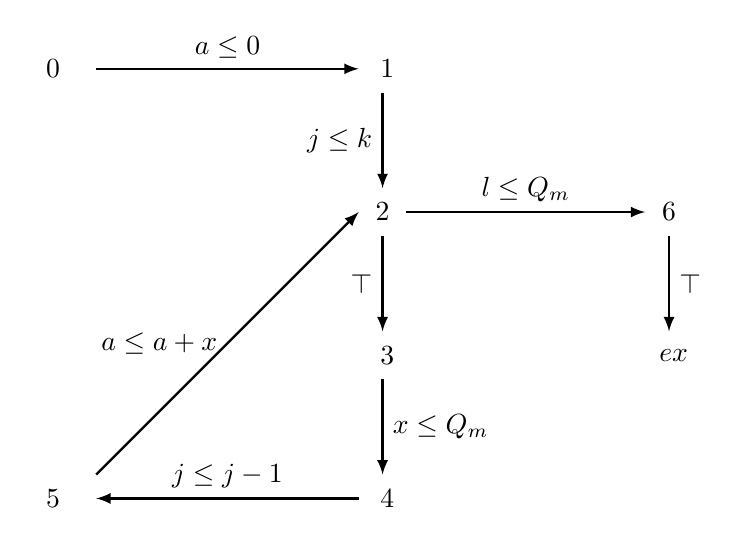
\begin{tikzpicture}[scale=\textwidth/20cm,samples=200]
  \draw[] (-7, 10) circle (0pt) node{{ $0$}};
  \draw[] (0, 10) circle (0pt) node{{ $1$}};
  \draw[] (0, 7) circle (0pt) node{\textbf{$2$}};
  \draw[] (0, 4) circle (0pt) node{{ $3$}};
  \draw[] (0, 1) circle (0pt) node{{ $4$}};
  \draw[] (-7, 1) circle (0pt) node{{ $5$}};
  % Counter Variables
  \draw[] (6, 7) circle (0pt) node {\textbf{$6$}};
  \draw[] (6, 4) circle (0pt) node {{ $ex$}};
  %
  % Control Flow Edges:
  \draw[ thick, -latex] (-6, 10)  -- node [above] {$a \leq 0$}(-0.5, 10);
  \draw[ thick, -latex] (0, 9.5)  -- node [left] {$j \leq k$} (0, 7.5) ;
  \draw[ thick, -latex] (0, 6.5)  -- node [left] {$\top$}  (0, 4.5);
  \draw[ thick, -latex] (0, 3.5)  -- node [right] {$x \leq Q_m$} (0, 1.5) ;
  \draw[ thick, -latex] (-0.5, 1)  -- node [above] {$j \leq j - 1$} (-6, 1) ;
  \draw[ thick, -latex] (-6, 1.5)  -- node [left] {$a \leq a + x$} (-0.5, 7)  ;
  \draw[ thick, -latex] (0.5, 7)  -- node [above] {$l \leq Q_m$}  (5.5, 7);
  \draw[ thick, -latex] (6, 6.5)  -- node [right] {$\top$} (6, 4.5) ;
  \end{tikzpicture}
  \caption{}
    \end{centering}
    \end{subfigure}
    \begin{subfigure}{.45\textwidth}
      \begin{centering}
    %   \todo{abstract-cfg for two round}
    \begin{tikzpicture}[scale=\textwidth/20cm,samples=200]
    \draw[] (-10, 10) circle (0pt) node{{ $0: 1$}};
    \draw[] (0, 10) circle (0pt) node{{ $1: 1$}};
    \draw[] (0, 7) circle (0pt) node{\textbf{$2: k$}};
    \draw[] (0, 4) circle (0pt) node{{ $3: k$}};
    \draw[] (0, 1) circle (0pt) node{{ $4: k$}};
    \draw[] (-10, 1) circle (0pt) node{{ $5: k$}};
    % Counter Variables
    \draw[] (6, 7) circle (0pt) node {\textbf{$6: 1$}};
    \draw[] (6, 4) circle (0pt) node {{ $ex: 1$}};
    %
    % Control Flow Edges:
  \draw[ thick, -latex] (-8, 10)  -- node [above] {$a \leq 0$}(-1.5, 10);
  \draw[ thick, -latex] (0, 9.5)  -- node [left] {$j \leq k$} (0, 7.5) ;
  \draw[ thick, -latex] (0, 6.5)  -- node [left] {$\top$}  (0, 4.5);
  \draw[ thick, -latex] (0, 3.5)  -- node [right] {$x \leq Q_m$} (0, 1.5) ;
  \draw[ thick, -latex] (-1.5, 1)  -- node [above] {$j \leq j - 1$} (-8, 1) ;
  \draw[ thick, -latex] (-8, 1.5)  -- node [left] {$a \leq a + x$} (-1.5, 7)  ;
  \draw[ thick, -latex] (1.5, 7)  -- node [above] {$l \leq Q_m$}  (4.5, 7);
  \draw[ thick, -latex] (6, 6.5)  -- node [right] {$\top$} (6, 4.5) ;
    \end{tikzpicture}
    \caption{}
      \end{centering}
      \end{subfigure}
    \caption{(a) The same $\kw{towRounds(k)}$ program as Figure~\ref{fig:twoRounds_example}
    (b) The abstract control flow graph for $\kw{towRounds(k)}$  (c) The abstract control flow graph with the reachability bound for $\kw{towRounds(k)}$.}
    \vspace{-0.5cm}
    \label{fig:abscfg_tworound}
  \end{figure}
\end{example}

\subsubsection{Static Data Dependency Analysis}
\label{subsubsec:static-datadep}
The new data dependency relation analysis algorithm
is performed on basis of the standard control flow graph.
\highlight{Improved from previous analysis,
this new analysis algorithm combines the reaching definition analysis into the standard data flow analysis.
It designs an improved version of data flow analysis named feasible 
data-flow, estimating a tighter bound on the data dependency relation. 
}
%  of the program, called abstract control flow graph.
In this part, I first show how to generate the standard abstract control flow graph in
Section~\ref{sec:static-cfg}
Then in Section~\ref{sec:static-feasible_flowsto}, 
I present the new feasible 
data-flow analysis
%  reachability-bound analysis algorithm adapted from the newly-designed
% technique in Chapter~\ref{sec:reachability-analysis} 
for estimating the data dependency relation.
Section~\ref{sec:static-dep_compute}
uses the reachability-bound analysis results estimating the dependency quantity
over labeled variables.
%  and
% Section~\ref{sec:static-quantity-edge} uses the same information
% estimating the dependency quantity for the pairs of dependent variables.
In Appendix~\ref{apdx:flowsto_soundness_extend},
this static algorithm is proved as the sound approximation of the variable \emph{may-dependency} relation
in the execution-based analysis in Section~\ref{sec:dynamic-datadep}.
%  before the introduction of  the edge and weight estimation.  

\subsubsection{Standard Control Flow graph}
\label{sec:static-cfg}
% Another operator \mathsf{blocks} 
The standard control flow graph is generated through following steps.
\paragraph*{Vertices Construction}
The vertices of this graph is the set of $c$'s labels , 
\[ 
  \cfgV(c) = labels(c)
\]
%
% Performing a feasible data-flow analysis through the reachable definition algorithm. 
%  By generating set of all the reachable variables at location of label $l$ in the program $c$.
% For every labelled variable $x^l$ in this set, 
% the value assigned to that variable
% in the assignment command associated to that label is reachable at the entry point of  executing the command of label $l$.
\paragraph*{Edges Construction}
The edges set is constructed in following steps.
\\
\textbf{Initial State:}
%
$\cfginit(c) \in \ldom$.
\\
The \emph{initial state} for a program $c$ is the initial label of this program.
This label corresponds to the first labeled command of this program 
when executing this program.
\\
Given a program $c$, its abstract initial state is computed as follows,
%
\[
  \begin{array}{ll}
    \cfginit(\clabel{\assign{x}{\expr}}{}^l)  & = l  \\
    \cfginit(\clabel{\assign{x}{\query(\qexpr)}}{}^l)  & = l \\
    \cfginit(\clabel{\eskip}^{l})  & = l \\
    \cfginit(\eif [b]^l \ethen c_1 \eelse c_2)  & = l \\
    \cfginit(\ewhile [b]^l \edo c)  & = l \\
    \cfginit(c_1 ; c_2)  & = \cfginit(c_1) \\
 \end{array}
 \]
%

\textbf{Final State}: $\cfgfinal(c) \in \mathcal{P}(\ldom)$
The \emph{Final State} of the program $c$, 
$\cfgfinal(c) \in \mathcal{P}(\ldom)$
is a set of labels.
Every label in $\cfgfinal(c)$ corresponds to the exist point of $c$.
\\
Given a program $c$, its final state is computed as follows,
% computes the set of Final State for the command. 
 \[
  \begin{array}{ll}
    \cfgfinal(\clabel{\assign{x}{\expr}}{}^l)  & = \{l\}  \\
     \cfgfinal(\clabel{\assign{x}{\query(\qexpr)}}{}^l)  & = \{l\}  \\
     \cfgfinal(\clabel{\eskip}^{l})  & = \{l\} \\
     \cfgfinal(\eif [b]^l \ethen c_1 \eelse c_2)  & = \cfgfinal(c_1) \cup \cfgfinal(c_2) \\
     \cfgfinal(\ewhile [b]^l \edo c)  & = \{l\} \\
     \cfgfinal(c_1 ; c_2)  & =  \cfgfinal(c_2) 
 \end{array}
 \]

The control flow graph is generated by edges between labels. 
Define $\cfgflow(c): \mathcal{P}(\ldom \times \ldom)$.
%
\[
 \begin{array}{ll}
    \cfgflow(\clabel{\assign{x}{\expr}}{}^l)  & = \emptyset  \\
    \cfgflow(\clabel{\assign{x}{\query(\qexpr)}}{}^l)   & = \emptyset  \\
    \cfgflow(\clabel{\eskip}^{l})  & = \emptyset \\
    \cfgflow(\eif [b]^l \ethen c_1 \eelse c_2) & =  \cfgflow(c_1) \cup \cfgflow(c_2)\cup \{(l, \cfginit(c_1)) , (l, \cfginit(c_2)) \} \\
    \cfgflow(\ewhile [b]^l \edo c)  & =  \cfgflow(c) \cup \{(l, \cfginit(C)) \} \cup \{(l', l)| l' \in \cfgfinal(c) \} \\
    \cfgflow(c_1 ; c_2)  & = \cfgflow(c_1) \cup  \cfgflow(c_2) \cup \{ (l, \cfginit(c_2)) | l \in \cfgfinal(c_1) \} \\
 \end{array}
 \]

The edges for the control flow graph is generated as follows.
Then, I build the edge for $c$'s abstract control flow graph as follows,
\[
  \cfgE(c) = \{(l_1, l_2) | (l_1, l_2) \in \cfgflow(c)\}
  \]

%  I have a pre-processing algorithm to go through the programs and returns the list of labels associating with a loop and whose visiting times need to be analyzed.
%


\paragraph{Control Flow Graph} 
With the vertices $\cfgV(c)$ and edges $\cfgE(c)$ ready, I construct the abstract control flow graph, formally 
% Through a program $c$'s abstract execution trace, its abstract control flow graph is computed 
defined in 
Definition~\ref{def:abs_cfg}.
% Given program $c$ with its abstract control flow $\cfgflow(c)$, the Abstract Control Flow Graph:
% \\
\begin{defn}[Control Flow Graph]
\label{def:cfg_graph}
Given a program $c$, 
with its abstract control flow $\cfgflow(c)$
its abstract control flow graph $\cfgG(c) =(\cfgV(c), \cfgE(c))$ is defined as follows,
\\
% \highlight{
% :
%
% \\
$\cfgE(c) = \{(l_1, dc, l_2) | (l_1, dc, l_2) \in \cfgflow(c)\}$,
\\
$\cfgV(c) = labels(c)$
% }
% \\
% , where the weight of every label to be computed in the next step.
\end{defn}




\subsubsection{Feasible Data-Flow Analysis}
\label{sec:static-feasible_flowsto}
I develop a variant of data flow analysis, called Feasible Data-Flow Generation, which 
considers both the control flow and data flow and
is a sound approximation of the edges in the execution based dependency graph.

% \wq{
\highlight{Improved from previous analysis,
this new analysis algorithm combines the reaching definition analysis on the control flow graph in feasible 
data-flow generation to have a more precise approximation. 
}
% }

% In this step, through 
% % the vertices and edges in 
% $c$'s abstract contrl flow graph $\cfgG(c)$,
%  $\THESYSTEM$ performs a feasible data-flow analysis 
%  using the reachable definition algorithm,
% %  and then Then I generated the set of feasible data-flow between labeled variables based on that.
% and generates the 
% %set of 
% feasible data-flow relation between labeled variables.
% \\
%  By generating set of all the reachable variables at location of label $l$ in the program $c$.
% For every labelled variable $x^l$ in this set, 
% the value assigned to that variable
% in the assignment command associated to that label is reachable at the entry point of  executing the command of label $l$.
% \\
It first defines some operations and then
% In the first step, 
% it 
performs the standard reaching definition analysis given a program $c$, 
on 
% its every label $l$
every label in $\cfgV(c)$.  
% \\
% it performs the standard reaching definition analysis given a program $c$, on its every label $l$.
% \\
% Another operator \mathsf{blocks} 
%
% Performing a feasible data-flow analysis through the reachable definition algorithm. 
%  By generating set of all the reachable variables at location of label $l$ in the program $c$.
% For every labelled variable $x^l$ in this set, 
% the value assigned to that variable
% in the assignment command associated to that label is reachable at the entry point of  executing the command of label $l$.
% \paragraph{Generate CFG}
%  \begin{def}
%   \label{def:init_label}
%   Define $\mathsf{init}$: Command -> label, which returns the initial label of the statement. 
% \[
%  \begin{array}{ll}
%     init([x := e]^{l})  & = l  \\
%      init([x := q(e)]^{l})  & = l \\
%      init([skip]^{l})  & = l \\
%      init([if [b]^l then C_1 else C_2]^{l})  & = l \\
%      init([while [b]^l do C]^{l})  & = l \\
%      init(C_1 ; C_2)  & = init(C_1) \\
%  \end{array}
%  \]
% \end{def}
%   Define $\mathsf{final}$: Command -> Powerset(label), which returns the final labels of the statement. 
%  \[
%  \begin{array}{ll}
%     final([x := e]^{l})  & = \{l\}  \\
%      final([x := q(e)]^{l})  & = \{l\}  \\
%      final([skip]^{l})  & = \{l\} \\
%      final([if [b]^l then C_1 else C_2]^{l})  & = final(C_1) \cup final(C_2) \\
%      final([while [b]^l do C]^{l})  & = \{l\} \footnote{while terminates after b evaluates to false} \\
%      final(C_1 ; C_2)  & =  final(C_2) \\
%  \end{array}
%  \]
% \paragraph*{Blocks and Defs}
%  Define block B to be either the command of the form of assignment, skip, or test of the form of $[b]^{l}$.\\
%  Define $\mathsf{blocks}$ : command -> Powerset(Block)
%  \[
%  \begin{array}{ll}
%     blocks([x := e]^{l})  & = \{[x := e]^{l}\}  \\
%      block([x := q(e)]^{l})  & = \{[x := q(e)]^{l}\}  \\
%      blocks([skip]^{l})  & = \{[skip]^{l}\} \\
%      blocks([if [b]^l then C_1 else C_2]^{l})  & = {[b]^{l}} \cup blocks(C_1) \cup blocks(C_2) \\
%      blocks([while [b]^l do C]^{l})  & = \{[b]^{l}\} \cup blocks(C) \\
%      blocks(C_1 ; C_2)  & = blocks(C_1) \cup  blocks(C_2) \\
%  \end{array}
%  \]
%  Define $\mathsf{labels}$ to get the labels of blocks.
%  \[
%    labels(C) = \{l | [B]^{l} \in blocks(C) \}
%  \]  

% The control flow graph is generated by edges between labels. Define $\mathsf{flow}$: command -> P (label $\times$ label ).

% \[
%  \begin{array}{ll}
%     flow([x := e]^{l})  & = \emptyset  \\
%      flow([x := q(e)]^{l})  & = \emptyset  \\
%      flow([skip]^{l})  & = \emptyset \\
%      flow([if [b]^l then C_1 else C_2)  & =  flow(C_1) \cup flow(C_2)\cup \{(l, init(C_1)) , (l, init(C_2)) \} \\
%      flow([while [b]^l do C)  & =  flow(C) \cup \{(l, init(C)) \} \cup \{(l', l)| l' \in final(C) \} \\
%      flow(C_1 ; C_2)  & = flow(C_1) \cup  flow(C_2) \cup \{ (l,init(C_2)) | l \in final(C_1) \} \\
%  \end{array}
%  \]
 
%  Define block B to be either the command of the form of assignment, skip, or test of the form of $[b]^{l}$.\\
%  Define $\mathsf{blocks}$ : command -> Powerset(Block)
\paragraph*{Blocks and Defs}
The block, 
is either the command of the form of assignment, skip, or a test of the form of $[b]^{l}$, 
% and $block$ of program $c$ is 
denoted by $\mathsf{blocks}(c)$
the set of all the blocks 
in program $c$, where  $\mathsf{blocks}: \cdom \to \mathcal{P}(\cdom \cup \clabel{\bexpr}^{l})$.
Then it generates the set of feasible data-flow between labeled variables with detail in Definition~\ref{def:feasible_flowsto}, 
based on $\live(l, c)$ for every label in a program $c$ and its blocks $\mathsf{blocks}$.
\\
The details are as follows.

The operator $\mathsf{blk} : \cdom \to \mathsf{blocks}$ gives all the blocks in program $c$.
\\
 \[
 \begin{array}{ll}
  \mathsf{blk}(\clabel{\assign{x}{\expr}}{}^l)  & = \{(\clabel{\assign{x}{\expr}}{}^l)\}  \\
  \mathsf{blk}(\clabel{\assign{x}{\query(\qexpr)}}{}^l)  & = \{(\clabel{\assign{x}{\query(\qexpr)}}{}^l)\}  \\
  \mathsf{blk}([\eskip]^{l})  & = \{[\eskip]^{l}\} \\
  \mathsf{blk}(\eif [b]^l \ethen c_1 \eelse c_2)  & = {[b]^{l}} \cup \mathsf{blk}(c_1) \cup \mathsf{blk}(c_2) \\
  \mathsf{blk}(\ewhile [b]^l \edo c)  & = \{[b]^{l}\} \cup \mathsf{blk}(c) \\
  \mathsf{blk}(C_1 ; C_2)  & = \mathsf{blk}(c_1) \cup  \mathsf{blk}(c_2) \\
 \end{array}
 \]
%  $label^{?}$ is label $\cup \{?\}$.\\
%  Define $\mathsf{kill}$: $blocks \to \mathcal{P}(\mathcal{VAR} \times LABEL \cup \{?\})$, which produces the set of labelled variables of assignment destroyed by the block.
\paragraph*{Kills and Gens}
The operator $\mathsf{kill}$: $\mathsf{blocks} \to \mathcal{P}(\mathcal{VAR} \times \ldom \cup \{?\})$ produces the set of labelled variables of assignment destroyed by the block.
 \\
  % Define $\mathsf{gen}$: $blocks \to \mathcal{P}(\mathcal{VAR} \times LABEL \cup \{?\})$, which generates the set of labelled variables generated by the block.
  The operator $\mathsf{gen}$: $\mathsf{blocks} \to \mathcal{P}(\mathcal{VAR} \times \ldom \cup \{?\})$ generates the set of labelled variables generated by the block.
  \\
  % Define $defs(x)(c): \mathcal{VAR} \to LABEL$, gives all the labels where assigns value to variable x in the target program $c$. 
  % The operator  $defs(c): \mathcal{VAR} \to \ldom$ gives all the labels where assigns value to variable in $c$. 
 \[
 \begin{array}{ll}
  \mathsf{kill}(\clabel{\assign{x}{\expr}}{}^l)  & = \{ (x, ?) \} \cup \{ (x, l') | l' \in defs(x) \} \\
  \mathsf{kill}(\clabel{\assign{x}{\query(\qexpr)}}{}^l)  & = \{ (x, ?) \} \cup \{ (x, l') | l' \in defs(x) \}  \\
  \mathsf{kill}([\eskip]^{l})  & = \emptyset \\
  \mathsf{kill}([ [b]^l ]^{l})  & =  \emptyset
 \end{array}
 ~~
  \begin{array}{ll}
    \mathsf{gen}(\clabel{\assign{x}{\expr}}{}^l)  & = \{ (x, l) \}  \\
    \mathsf{gen}(\clabel{\assign{x}{\query(\qexpr)}}{}^l)  & = \{ (x, l) \}  \\
    \mathsf{gen}([\eskip]^{l})  & = \emptyset \\
    \mathsf{gen}([ [b]^l ]^{l})  & =  \emptyset 
 \end{array}
 \]
 The $?$ is a placeholder for the unknown label need to be comptued.
%  Define $in(l)$, $out(l)$: LABEL$ \to \mathcal{VAR} \times LABEL \cup \{?\}$ for every block in program $c$ is computed as follows,
%  \[
%  \begin{array}{lll}
%     in(l)  & = \{ (x, ?) | x^l \in \lvar_c \land  l = \cfginit(c) \}  
%     \cup \{ out(l')|  | (l',\_, l) \in \cfgE \land  l \neq \cfginit(c)\}  \\
%      out(l)  & =  gen(B^{l}) \cup \{ in(l) \setminus kill(B^l)  \} & B^l \in blocks(c)   
%  \end{array}
%  \]
%  computing $in(l)$ and $out(l)$ for every $B^l \in blocks(c) $, and repeating these two step
% until the $in(l)$ and $out(l)$ are stabilized for every $B^l \in blocks(c) $
%  I use $\live_{in}(l,c)$ and $\live_{out}(l, c)$ denote the stabilized results for the command of label $l$ in program $c$. 
%  Define $defs(x)(c): \mathcal{VAR} \to LABEL$, gives all the labels where assigns value to variable x in the target program $c$.
% Define $defs(x)(c): \mathcal{VAR} \to \ldom$, gives all the labels where assigns value to variable x in the target program $c$.
% \\
%  Define $in(l)$, $out(l)$: $ \ldom \to \mathcal{VAR} \times LABEL \cup \{?\}$ for every block in program $c$ is computed as follows,
\paragraph*{In and Out}
The operator  $in(l)$, $out(l)$: $ \ldom \to \mathcal{LV} \cup \{?\}$ for every block in program $c$ is defined as follows,
 \[
 \begin{array}{ll}
    % in(l)  & = \{ (x, ?) | x^l \in \lvar_c \land  l = \cfginit(c) \}  
    in(l)  & = \{ x^{?} | x^l \in \lvar_c \land  l = \cfginit(c) \}  
    \cup \{ out(l')|  | (l',\_, l) \in \cfgE(c) \land  l \neq \cfginit(c)\}  \\
     out(l)  & =  \mathsf{gen}(B^{l}) \cup \{ in(l) \setminus \mathsf{kill}(B^l)  \}  
 \end{array}
 \]
computing $in(l)$ and $out(l)$ for every $B^l \in \mathsf{blk}(c) $, and repeating these two steps
until the $in(l)$ and $out(l)$ are stabilized for every $B^l \in \mathsf{blk}(c) $
%  I use $\live_{in}(l,c)$ and $\live_{out}(l, c)$ denote the stabilized results for the command of label $l$ in program $c$. 
 I use $\live(l,c)$ to represent 
% $\live_{in}(l,c)$ in the other part of the paper.
denote the stabilized result of $in(l)$ at label $l$ in program $c$. 
% The $\live_{in}(l,c)$ and $\live_{out}(l, c)$ is computed by the Standard worklist algorithm. (For simplicity, I use $\live(l,c)$ to represent $\live_{in}(l,c)$ in the other part of the paper.}
\\
% The $\live_{in}(l,c)$ and $\live_{out}(l, c)$ 
\paragraph{Reaching definition computation}
This step generates set of all the reachable variables at location of label $l$ in the program $c$.
The $\live(l, c)$ represent the analysis result, which is the set of 
reachable labeled variables in program $c$ at the location of label $l$.
For every labelled variable $x^l$ in this set, 
the value assigned to that variable
in the assignment command associated to that label is reachable at the entry point of  executing the command of label $l$.

The stabilized $in(l)$ and $out(l)$ for program $c$, as well as $\live(l, c)$,
is computed by the standard worklist algorithm with detail as below. 
% For simplicity, I use $\live(l,c)$ to represent $\live_{in}(l,c)$ in the other part of the paper.
\begin{enumerate}
    \item Initializing in[l]=out[l]=$\emptyset$
    \item Initializing in[entry label] = $\emptyset$
    \item Initializing a work queue, contains all the blocks in $c$
    \item while |W| != 0 \\
         pop l in W\\
          old = out[l]\\
          in(l) =  out(l') where $(l',\_, l) \in \cfgE(c)$\\
           out(l) = $\mathsf{gen}$($b^l$) $\cup$ (in(l) - $\mathsf{kill}$($b^l$) ) where $b^l$ in $\mathsf{blk}(c)$   \\
          if (old != out(l)) W= W $\cup$ \{l'| (l,l') in $(l',\_, l) \in \cfgE(c)$\}\\
          end while
\end{enumerate}
%
% computing $in(l)$ and $out(l)$ for every $B^l \in blocks(c) $, and repeating these two step
% until the $in(l)$ and $out(l)$ are stabilized for every $B^l \in blocks(c) $
%  I use $\live_{in}(l,c)$ and $\live_{out}(l, c)$ denote the stabilized results for the command of label $l$ in program $c$. 
% The $\live_{in}(l,c)$ and $\live_{out}(l, c)$ is computed by the Standard worklist algorithm. (For simplicity, I use $\live(l,c)$ to represent $\live_{in}(l,c)$ in the other part of the paper.
%%
\paragraph{Feasible Data-Flow Generation}
by using the results of Reaching definition analysis results, specifically $\live(l, c)$ for every label in a program $c$, I refine the vertices and edges in the $\cfgG$ graph 
by generating the set of feasible data-flow between labeled variables as follows,
%
%   \[
%  \begin{array}{ll}
%     dcdg([x := e]^{l})  & = \{ (y^i, x^l) | y \in VAR(e) \land (y,i) \in \live_{in}(l) \}  \\
%      dcdg([x := q(e)]^{l})  & = \{ (y^i, x^l) | y \in VAR(e) \land (y,i) \in \live_{in}(l) \}  \\
%      dcdg([skip]^{l})  & = \emptyset \\
%      dcdg([if [b]^l then C_1 else C_2)  & =  dcdg(c_1) \cup dcdg(c_2)\\ & \cup \{(x^i,y^j) | x \in VAR(b) \land (x,i) \in \live_{in}(l) \land ([y = \_]^j) \in blocks(c_1) \} \\
%      &\cup \{(x^i,y^j) | x \in VAR(b) \land (x,i) \in \live_{in}(l) \land ([y = \_]^j) \in blocks(c_2) \} \\
%      dcdg([while [b]^l do c)  & =  dcdg(c) \cup \{(x^i,y^j) | x \in VAR(b) \land (x,i) \in \live_{in}(l) \land ([y = \_]^j) \in blocks(C) \} \\
%      dcdg(c_1 ;c_2)  & = dcdg(c_1) \cup  dcdg(c_2) \\
%  \end{array}
%  \]
%
\begin{defn}[Feasible Data-Flow]
  \label{def:feasible_flowsto}
  Given a program $c$ and two labeled variables $x^i, y^j$  in this program, 
  $\flowsto(x^i, y^j, c)$ is 
    {\footnotesize
    \[
   \begin{array}{ll}
    \flowsto(x^i, y^j, \clabel{\assign{x}{\expr}}{}^l)  & \triangleq (x^i, y^j) \in \{ (y^i, x^l) | y \in \mathsf{FV}(\expr) 
    % \land (y,i) \in \live(l, \clabel{\assign{x}{\expr}}^l) \}  \\
    \land y^i \in \live(l, \clabel{\assign{x}{\expr}}^l) \}  \\
    \flowsto(x^i, y^j, \clabel{\assign{x}{\query(\qexpr)}}{}^l)  & \triangleq (x^i, y^j) \in \{ (y^i, x^l) | y \in \mathsf{FV}(\qexpr) 
    % \land (y,i) \in \live(l,\clabel{\assign{x}{\query(\qexpr)}}^l) \}  \\
    \land y^i \in \live(l,\clabel{\assign{x}{\query(\qexpr)}}^l) \}  \\
    \flowsto(x^i, y^j, [\eskip]^{l})  & = \emptyset \\
    \flowsto(x^i, y^j, \eif ([b]^l, c_1, c_2))  & \triangleq \flowsto(x^i, y^j, c_1) \lor \flowsto(x^i, y^j, c_2) \\ 
        & \lor (x^i, y^j) \in
       \{(x^i,y^j) | x \in \mathsf{FV}(b) \land 
      %  (x,i) 
      x^i \in \live(l, \eif ([b]^l, c_1, c_2)) \land  y^j \in \lvar(c_1) \\
    %   ([y = \_]^j) \in \mathsf{blk}(c_1) \} \\
       &\lor (x^i, y^j) \in \{(x^i,y^j) | x \in \mathsf{FV}(b) \land 
      %  (x,i) 
      x^i\in \live(l, \eif ([b]^l, c_1, c_2))  \land  y^j \in \lvar(c_2) \\
    %   \land ([y = \_]^j) \in \mathsf{blk}(c_2) \} \\
       \flowsto(x^i, y^j, \ewhile [b]^l \edo c_w)  & \triangleq  \flowsto(x^i, y^j, c_w)  \lor
       \\ & 
       (x^i, y^j) \in  \{(x^i,y^j) | x \in \mathsf{FV}(b) \land 
      %  (x,i) 
      x^i \in \live(l,   \ewhile [b]^l \edo c_w) \land  y^j \in \lvar(c_w) \\
    %   ([y = \_]^j) \in \mathsf{blk}(c_w) \} \\
       \flowsto(x^i, y^j, c_1 ;c_2)  & \triangleq \flowsto(x^i, y^j, c_1) \lor \flowsto(x^i, y^j, c_2) \\
   \end{array}
   \]
   }
   \end{defn}
%
This \emph{Feasible Data-Flow} relation is a sound approximation 
of the variable \emph{May-Dependency} relation over labeled variables for every program.
The soundness is proved
in Appendix~\ref{apdx:flowsto_soundness}.
%
\subsubsection{Data Dependency Relation Estimation}
\label{sec:static-dep_compute}
%
For any program $c$ and two labeled variables $x^i, y^j$  in this program, 
$x^i, y^j$  is in the estimated dependency relation if and only if they satisfy
$\flowsto(x^i, y^j, c)$.

As introduce in the third step in Section~\ref{sec:static-overview},
this set is used in Section~\ref{sec:static-adapt} to estimate
the execution-based dependency graph.
As introduced in third step of this analysis framework in Section~\ref{sec:static-overview},
this information will be used in constructing the program-based dependency graph, to estimate the execution-based dependency graph for the program.
For easy understanding,
I reveal the estimated directed edges construction below
% vertex and weight construction of this estimated graph below
and presents the formal definition later. 
% for each vertex in $\progV(c)$,
This estimated directed edges set is defined as a set of triples 
% $\progW(c) \in \mathcal{P}(\mathcal{LV} \times \mathcal{LV} \times EXPR(\constdom))$ 
$\progE(c) \in \mathcal{P}(\mathcal{LV} \times \mathcal{A}_{\lin} \times \mathcal{LV})$,
Each directed edge is defined between vertices $({x}_1^{i}, w_1)$  
and $({x}_2^{j}, w_2)$ 
where ${x}_1^{i}, {x}_2^{j} \in \lvar(c)$, and they are in the estimated dependency relation
% is the set of pairs 
% The weight for each vertex in $\progV(c)$ is computed 
% indicating a directed edge from the first vertex to the second one in each pair
as follows,
\highlight{
  \[
    \progE^0(c) \triangleq 
    \left\{ 
    ({x}_1^{i}, w, {x}_2^{j}) \in \mathcal{LV} \times 
    \mathcal{A}_{\kw{in}} \times \mathcal{LV}
    ~ \middle\vert ~
    \begin{array}{l}
      {x}_1^{i}, {x}_2^{j} \in \lvar(c)
    \land
      % \\
      \exists n \in \mathbb{N}, z_1^{r_1}, \cdots, z_n^{r_n} \in \lvar_{{c}} \sthat
      n \geq 0 \land
      \\
      \flowsto(x^i,  z_1^{r_1}, c) 
      \land \cdots \land \flowsto(z_n^{r_n}, y^j, c) 
    \end{array}
    \right\}
    \]
}
The weight $w$ for every edge in this definition is a placeholder.
It will be computed in Section~\ref{sec:static-quantity}.
We prove that this estimated directed edge set $\progE(c)$ is a sound approximation of the 
edge set in $c$'s Execution-Based Dependency Graph 
in Appendix~\ref{apdx:adapt_soundness}.

% \paragraph*{Edges Estimation}
% Then I define the estimated directed edges
% % for each vertex in $\progV(c)$,
% between vertices in $\progV(c)$,
% as a set of pairs 
% % $\progW(c) \in \mathcal{P}(\mathcal{LV} \times \mathcal{LV} \times EXPR(\constdom))$ 
% $\progE(c) \in \mathcal{P}(\in \mathcal{LV} \times \mathcal{LV})$
% % is the set of pairs 
% % The weight for each vertex in $\progV(c)$ is computed 
% indicating a directed edge from the first vertex to the second one in each pair
% as follows,
% \highlight{
%   \[
%     \progE(c) \triangleq 
%     \left\{ 
%     ({x}_1^{i}, {x}_2^{j}) \in \mathcal{LV} \times \mathcal{LV}
%     ~ \middle\vert ~
%     \begin{array}{l}
%       {x}_1^{i}, {x}_2^{j} \in \progV(c)
%     \land
%       % \\
%       \exists n \in \mathbb{N}, z_1^{r_1}, \cdots, z_n^{r_n} \in \lvar_{{c}} \sthat  
%       n \geq 0 \land
%       \\
%       \flowsto(x^i,  z_1^{r_1}, c) 
%       \land \cdots \land \flowsto(z_n^{r_n}, y^j, c) 
%     \end{array}
%     \right\}
%     \]
% }
% This estimated directed edge set $\progE(c)$ is a sound approximation of the 
% edge set in $c$'s execution-based dependency graph, which is proved 
% in Appendix~\ref{apdx:adapt_soundness}.
%  \begin{defn}[Feasible Data-Flow]
%   \label{def:feasible_flowsto}
%     {\footnotesize
%     \[
%    \begin{array}{ll}
%       dcdg(\clabel{\assign{x}{\expr}}{}^l)  & = \{ (y^i, x^l) | y \in FV(e) \land (y,i) \in \live_{in}(l, \clabel{\assign{x}{\expr}}^l) \}  \\
%        dcdg(\clabel{\assign{x}{\query(\qexpr)}}{}^l)  & = \{ (y^i, x^l) | y \in FV(e) \land (y,i) \in \live_{in}(l,\clabel{\assign{x}{\query(\qexpr)}}^l) \}  \\
%        dcdg([\eskip]^{l})  & = \emptyset \\
%        dcdg([\eif [b]^l \ethen c_1 \eelse c_2)  & =  dcdg(c_1) \cup dcdg(c_2)\\ & \cup 
%        \{(x^i,y^j) | x \in FV(b) \land (x,i) \in \live_{in}(l) \land ([y = \_]^j) \in blocks(c_1) \} \\
%        &\cup \{(x^i,y^j) | x \in FV(b) \land (x,i) \in \live_{in}(l) \land ([y = \_]^j) \in blocks(c_2) \} \\
%        dcdg([\ewhile [b]^l \edo c)  & =  dcdg(c) \cup \{(x^i,y^j) | x \in FV(b) \land (x,i) \in \live_{in}(l) \land ([y = \_]^j) \in blocks(C) \} \\
%        dcdg(c_1 ;c_2)  & = dcdg(c_1) \cup  dcdg(c_2) \\
%    \end{array}
%    \]
%    }
%    \end{defn}
%    For any two labeled variables $x^i, y^j$ in a program $c$, 
%   %  it is easy to see that there is a one-on-one correspondence between 
%   %  $\flowsto$ relation of the two variables, and the $dcdg$ analysis result on $c$.
%   I use $\flowsto()$ denote if they have a feasible data-flow relation in Definition~\ref{def:flowsto}.
%    \begin{defn}[Feasible Data-Flow ($\flowsto$)]
%    \label{def:flowsto}
%    \[
%    \forall c \in \cdom, x^i, y^j \in \lvar_c \sthat  
%    \flowsto(x^i, y^j, c) \iff (x^i, y^j) \in dcdg(c)
%    \]
%    \end{defn}
  %  This soundness is proved in Proof~\ref{pf:rd_soundness} in Appendix~\ref{apdx:rd_soundness}.
  %  For any two labeled variables in a program $c$, it is easy to see that there is a one-on-one correspondence between 
  %  $\flowsto$ relation of the two variables, and the $dcdg$ analysis result on $c$.
  %  \begin{thm}[Soundness of the Feasible Data-Flow Analysis]
  %  \label{thm:rd_soundness}
  %  \[
  %  \forall c \in \cdom, x^i, y^j \in \lvar_c \sthat  
  %  \flowsto(x^i, y^j, c) \iff (x^i, y^j) \in dcdg(c)
  %  \]
  %  \end{thm}
  %  This soundness is proved in Proof~\ref{pf:rd_soundness} in Appendix~\ref{apdx:rd_soundness}.
  \paragraph*{Example}
% Still looking at the Figure~\ref{fig:adapfun_tworound}(c), 
% and taking the edge $(l^6, a^5)$ for example.
% By $\flowsto(l^6, a^5, c)$, I can see $a$ is used directly in the query expression $\chi[k]*a$,
% in the assignment command $\clabel{\assign{l}{\query(\chi[k]*a)}}^l$,
% i.e., $a \in FV(\chi[k]*a)$.
% Also, from the Reaching definition analysis, I know $a^5 \in \live(6, two-round)$.
% Then I have $\flowsto(l^6, a^5, c)$ and construct the edge $(l^6, a^5)$.
% And same way for constructing the rest edges.
%
The edge $(l^6, a^5)$ in Figure~\ref{fig:twoRounds_example}(c) is constructed by this definition.
% and take  for example.
By $\flowsto(l^6, a^5, c)$, I can see $a$ is used directly in the query expression $\chi[k]*a$,
in the assignment command $\clabel{\assign{l}{\query(\chi[k]*a)}}^l$,
i.e., $a \in FV(\chi[k]*a)$.
Also, from the reaching definition analysis, I know $a^5 \in \live(6, \kw{twoRounds(k)})$.
Then I have $\flowsto(l^6, a^5, c)$ and construct the edge $(l^6, a^5)$.
And the same way for constructing the rest edges. Also, the edge $(x^3,j^5)$ in the same graph represents the control flow, 
caught by the $\flowsto$ relation.
% Still looking at the Figure~3(c) in main paper, 
% and taking the edge $(l^6, a^5)$ for example.
% By $\flowsto(l^6, a^5, c)$, I can see $a$ is used directly in the query expression $\chi[k]*a$,
% in the assignment command $\clabel{\assign{l}{\query(\chi[k]*a)}}^l$,
% i.e., $a \in FV(\chi[k]*a)$.
% Also, from the Reaching definition analysis, I know $a^5 \in \live(6, two-round)$.
% Then I have $\flowsto(l^6, a^5, c)$ and construct the edge $(l^6, a^5)$.
% And same way for constructing the rest edges. Also, the edge $(x^3,j^5)$ in the same graph represents the control flow, caught by our $\flowsto$ relation.
%
  \subsubsection{Improvements Analysis}
  \label{sec:static-dep-improvements}
  \highlight{
    This new data dependency estimation algorithm is more precise and efficient than previous static analysis.
% language and operational semantics design improves the expressiveness, efficiency, and the accuracy to a large extend.
% \todo{Add details}
\begin{itemize}
  %   \item \textbf{Improvements on Expressiveness}
  %   \\
  % This language is extended over the standard while language. 
  % In this sense, it supports all the general data analysis.
  \item \textbf{Improvements on Efficiency}
  \\
  New analysis architecture does not rewrite the program into SSA version.
\\
  New analysis technique does not pre-collect the variables generated during the program.
\\
  New analysis technique does unfold the while loop and perform analysis for each iteration of the loop, 
  instead, it only performs the analysis on the while body once.
  \\
In the three senses above, the efficiency is improved significantly.
  \item \textbf{Improvements on Accuracy}
  Comparing to previous dependency estimation method,
  new analysis technique uses the reachable definition algorithm.
  This algorithm improves the accuracy 
  on the approximating the data dependency relation.
  Let us see a simple example, a program $ [x = 0]^{1}; [x=2]^{2};  [y = x+1]^{3}$. 
The standard data flow analysis 
tells us that both the labeled variable $x^{1}$ and $x${2} may flow to $y^{3}$, which will result in an unnecessary edge ($x^{1}, y^{3}$). The result of reaching definition 
can help us eliminate this kind of edge by telling us, at line $3$, only variable $x^{2}$ is reachable. 
  \end{itemize}
  }

\subsubsection{Static Reachability Bound Analysis}
\label{subsubsec:static-reachability}

In order to estimate weight for every vertex in the program-based dependency graph,
we perform the symbolic reachability bound analysis on the abstract control flow graph and add weight as shown in Figure~\ref{fig:abscfg_tworound}(c). 
% This because
% the vertices in the two graph share the same unique label, the line number.
% We would like to generate the closure of every edge, which is an equality relation between variables.  Solving this closure gives us the reachability bound for this edge. With all the bound for all the edges in the abstract control flow graph, we can calculate the weight for every vertex in this graph. For example, we show the closure generated for the edge $(4, j < j - 1, 5)$, 
% $\absclr(4, 5) = \varinvar(j)$. The invariant for variable $j$, $\varinvar(j)$ used here is 
% $\varinvar(j) = k * \absclr(1, 2)$, which is generated by all the difference constraints involving $j$ in the graph. Notice the $k$ in $\varinvar(j)$ comes from considering both difference constraint $j<=k$ from edge (1,2) and $j<=j-1$ from (4,5), which intuitively reflects the while loop whose counter is set to $k$ at the beginning and decreases by 1 at each iteration.
% We first generate the invariant for every variable showing up in the difference constraint and not user defined. For example, in the Figure~\ref{def:abscfg_tworound}(b), there are three variables $a$, $x$, $j$ that we will generate invariant for. We show the invariant for the counter $k$, which is $j = k$. 
% $\absclr(1, 2) = 1$
% \\
% => 
% $\absclr(4, 5) = k$
% using the difference constraint on the edges for all 
% through the edges in $\absG(c)$, which correspond to $c$'s abstract transition between labels.
% We infer the invariant for every variable, and compute the transition closure for every abstract transition. By solving the closure
% with the invariants of variables involved in this closure for every transition, we compute
% the symbolic reachability bound of every commands corresponding to this transition. Specifically, this analysis can be performed in four steps:
%  Variable Modification Tracking, Local Bounds Computation,
% Invariant Inference and Closure Generation, and Reachability Bound Computation,
% 
% We present the details of invariant, closure generation, and reachability bound computation as follows.
% with details as follows.
% \\
% %
% 1.  Variable Modification Tracking: collecting the dc for where each variable is increased, decreased and reset: 
% \\
% 2. Local Bounds Computation: 
% \\
% 3. Invariant Inference and Closure Generation
% \\
% 4. Reachability Bound Computation,
% %
% \paragraph*{Variable Modification Tracking}
% Identify the abstract events where each variable is increased, decreased and reset:
% \\
% $\inc: \mathcal{VAR} \to \mathcal{P}(\absevent) $
% the set of the abstract events where the variable increase.
% \\
% $\inc(x) = \{(\absevent, c) | \absevent = (l, l', x' \leq x + v)\}$
% \\
% $\reset: \mathcal{VAR} \to \mathcal{P}(\absevent) $
% The set of the abstract events where the variable is reset.
% \\
% $\dec: \mathcal{VAR} \to \mathcal{P}(\absevent) $
% The set of abstract events where the variable decrease.
% % \\
% % $\dec(x) = \{(\absevent, c) | \absevent = (l, l', x' \leq x - v)\}$
% \\
% $Incr(v) \triangleq \sum\limits_{(\absevent, c) \in \inc(v)}\{\absclr(\absevent) \times v\}$
% %
% \paragraph*{Local Bounds}
% Given a program $c$ with its abstract control flow graph 
% $\absG(c) = (\absV, \absE)$
% \\
% Local Bounds Computation:
% $\locbound: \absevent \to \mathcal{VAR} \cup \constdom$.
% %
% \[ 
% \begin{array}{ll}
%   \locbound(\absevent) \triangleq 1 
%   & \absevent \notin SCC(\absG(c))
%   \\
%   \locbound(\absevent) \triangleq (x, v) 
%   & \absevent \in SCC(\absG(c)) \land \absevent \in \dec(x) \land  \absevent = (\_, \_ , x' \leq x - v) \\
%   \locbound(\absevent) \triangleq (x, \max(\dec(x))) 
%   & \absevent \in SCC(\absG(c)) \land 
%   \absevent  \notin \bigcup_{x \in \mathcal{VAR}} \dec(x)
%   \land \absevent \notin SCC(\absG(c) \setminus \dec(x)) 
% \end{array}
%   \]
%   The first case is straightforward. Since variable's visiting time outside of any while loop is at most 1, we do not need to analyze the visiting times of every node in the graph from phase 1.
%   The second and third step is guaranteed by the \emph{Discussion on Soundness} in Section 4 of \cite{sinn2017complexity}.
%   Then soundness proof is in Lemma~\ref{lem:local_bound_sound} in appendix~\ref{apdx:reachability_soundness}.
% %
% \paragraph*{Invariant Inference and Closure Generation }
% Then, computing the bound invariants for variables and the transition closures for abstract events:
% \\ 
% $ \varinvar: \mathcal{VAR} \cup \constdom \to EXPR(\constdom)$
% \\
% $\absclr: \absevent \to EXPR(\constdom)$
% \\
% Then, the symbolic invariant for each variable 
% as well as the symbolic transition closure for each transition is calculated as follows:
% \[ 
% \begin{array}{lll}
%   \varinvar(x) & \triangleq c & c \in \constdom \\
%   \varinvar(x) & \triangleq Incr(v) + \max(\{\varinvar(a) + c | (t, a, c) \in \reset(x)\}) & c \notin \constdom
% \end{array}
% \]
% %
% \begin{defn}
%   \label{def:transition_closure_base}
% \[ 
% \begin{array}{lll}
%   \absclr(\absevent) 
%   & \triangleq x / v & \\ 
%   & \locbound(\absevent) = (x, v) \in \constdom \times \mathbb{N} & \\
%   \absclr(\absevent) 
%   & \triangleq (Incr(x) + 
%   \sum\limits_{(\absevent', y, v') \in \reset(x)}
%   \absclr(\absevent') \times \max(\varinvar(y) + v', 0) ) / v & \\
%   & \locbound(\absevent) = (x, v) \land x \notin \constdom & 
% \end{array}
%   \]
% \end{defn}
% %
% \paragraph*{Improved Variable Modification Tracking}
% Instead of just identifying the abstract events where each variable is reset,
% this improvement identifies the chain of the events where a given variable is reset by the 
% variables of the abstract events through the chain.
% \\
% $\resetchain: \mathcal{VAR} \to \mathcal{P}(\mathcal{P}(\absevent)) $
% The set of the chain of abstract events where the variable is reset through the chain.
% % \\
% % $Incr(v) \triangleq \sum\limits_{(\absevent, c) \in \inc(v)}\{\absclr(\absevent) \times v\}$
% %
% \paragraph*{Improved Invariant Inference and Closure Generation}
% Then, computing the bound invariants for variables and the transition closures for abstract events:
% \\ 
% $ \varinvar: \mathcal{VAR} \cup \constdom \to EXPR(\constdom)$
% \\
% $\absclr: \absevent \to EXPR(\constdom)$
% \\
% Then, the symbolic invariant for each variable 
% as well as the symbolic transition closure for each transition is calculated as follows:
% \[ 
% \begin{array}{lll}
%   \varinvar(x) & \triangleq c & c \in \constdom \\
%   \varinvar(x) & \triangleq Incr(v) + \max(\{\varinvar(a) + c | (t, a, c) \in \reset(x)\}) & c \notin \constdom
% \end{array}
% \]
% %
% \begin{defn}
%   \label{def:transition_closure}
% \[ 
% \begin{array}{lll}
%   \absclr(\absevent) 
%   & \triangleq x / v & \\ 
%   & \locbound(\absevent) = (x, v) \in \constdom \times \mathbb{N} & \\
%   \absclr(\absevent) 
%   & \triangleq \Big(
%     \sum\limits_{y \in \{ y ~|~ 
%     ch \in \resetchain(x), (l_1, x, y, v, l_2) \in ch \} } Incr(x) & \\
%     & \quad + 
%   \sum\limits_{ch \in \resetchain(x)}
%   \big( \min\limits_{\absevent' \in ch}({\absclr(\absevent')}) \times 
%   \max(\varinvar(y) + \sum\limits_{(l_1, x, y, v, l_2) \in ch } v, 0)\big) \Big) / v & \\
%   & \locbound(\absevent) = (x, v) \land x \notin \constdom & 
% \end{array}
%   \]
% \end{defn}
  %
% \paragraph*{Adding the Reachability Bounds for Every Vertex in the Data-Control Flow Graph}
% Updating the weight of every vertex in the $\progG(c) = (\progV, \progE, \progW, \progF)$ for program $c$ generated from phase 1. 
% For every $x^l \in \progV$, find the abstract event $\absevent \in \absflow(c)$ of the form $(l, \_, \_)$, updating the $\progW(x^l) $ by the transition closure of this event.
% \\
% \paragraph*{Reachability Bound Computation}
% With all the closures for all the edges of the abstract control flow graph, we can solve them to obtains the reachability bound of every edges. We decide the weight for every vertex in the abstract control flow graph by using the bound of the edges which head out from this vertex, by taking the max of the bound from these involving edges. For instance,   
% By the constraint on the edge $(4, j \leq j - 1, 5)$, we get bound $k$ for this edge.
% Then, we assign vertex $4$ by reachability bound $k$, as in Figure~\ref{fig:abscfg_tworound}(c). 
% Another interesting vertex is $2$, which has more than one edge heading out from it, $(2, \top, 3)$ and $(2,\top, 6)$. For the weight for vertex $2$, we choose the max between the bound $k$ from $(2,\top, 3)$ and $1$ from $(2,\top, 6)$.
% we first infer its local bound as variable $j$.
% Then by solving the invariant for variable $j$,
% we infer the value bound for $j$, which is $k$.
% Then the reachability bound for this abstract transition, (i.e., edge $4, j \leq j - 1, 5$) 
% is computed as $k$ as well through Definition~\ref{def:abs_trace}.
% \\
% $
% \progW(x^l) 
%   \triangleq \absclr(\absevent)
% $
% Through the transition closure computed above, 
% The weight of every label in 
% % Then we update 
% the program $c$'s abstract control flow graph,
% $\absG(c) =(\absV, \absE, \absW)$
% is 
% computed as the maximum over all the abstract events $\absevent \in \absE$ heading out from this vertex, formally as follows.
% % by annotating each vertex with a symbolic weight. 
% % This weight corresponds to 
% %reachability bounds of
% \\
% $\absW 
% \triangleq \left\{ (l, w) \in \mathbb{N} \times EXPR(\constdom) | w = \max\limits_{\absevent = (l, \_, \_)} \{ \absclr(\absevent)\} \right\}$.
% % \\
% \paragraph*{Example}
% Still looking at the two-round example as in Figure~\ref{fig:abscfg_tworound}(b) where 
% each label $l$ is added with a weight by $absW$.
% This weight represents the  maximum reaching times of this location $l$, in the other word,
% the estimated maximum visiting times of the command labeled with $l$.
% For example, looking at the vertex $1$,
% by analysis steps, since it isn't in any SCC, it's estimated reachability bound is computed as $1$.
% However, for the vertex $4$ which is involved in an SCC, the reachability bound is inferred in another way.
% By the constraint on the edge $4, j \leq j - 1, 5$,
% we first infer its local bound as variable $j$.
% Then by solving the invariant for variable $j$,
% we infer the value bound for $j$, which is $k$.
% Then the reachability bound for this abstract transition, (i.e., edge $4, j \leq j - 1, 5$) 
% is computed as $k$ as well through Definition~\ref{def:abs_trace}.
% In this abstract control flow graph, every vertex is a label,
% corresponding to a label command in the program.
% Each directed 
% edge represents an abstract transition 
% between two control locations, 
% i.e., the labels of two commands (we call the labels also control location and they refer to the same thing), 
% where the second labeled command will be executed after execution of the command with first label.
% For example, the edge $0, a \leq 0, 1$ on the top, represents,
% from location $0$, the command 
% $\clabel{\assign{a}{0}}^0$ is executed with next continuation location $1$,
% where the 
% command $\clabel{\assign{j}{k}}^1$ will be executed next.
% The constraint $a \leq 0$ is generated by abstracting from the assignment command $\assign{a}{0}$,
% representing that value of $a$ is less than or equals to $0$ after 
% location $0$ before executing command at line $1$.
%
% The same way for the rest weights' computation.
We use $\absW(c)$ for the computed weights, 
a set of pairs 
$(l, w)$ where 
$w$ is the weight 
for label $l$ from the abstract control flow graph of $c$.
% The weight $w$ for each label $l$ 
$w$ is an arithmetic  expression over $\mathbb{N}$ and
input variables, denoted by $\mathcal{A}_{in}$.
This analysis is  inspired from the program complexity analysis method in \cite{sinn2017complexity}.
The detail of our symbolic reachability bound analysis which uses the difference constraint of the abstract control flow graph can be found in the appendix.
%
%
% \paragraph{Vertex Weight Computation}
% The weight for each vertex in $\progV(c)$ is computed as follows,
Then we compute the weight for each vertex in $\progV(c)$,
as a set of pairs $(x^l, w) \in \ldom \times \mathcal{A}_{in}$
% $\progW(c) \in \mathcal{P}(\mathcal{LV} \times \mathcal{LV} \times EXPR(\constdom))$ 
% is the set of pairs 
% The weight for each vertex in $\progV(c)$ is computed 
mapping each $x^l \in \progV(c)$ to an arithmetic  expression over $\mathbb{N}$ and
input variables. 
Because
the vertices in the two graph share the same unique label, the line number of the same command,
we define $\progW(c)$
% denoted by $\mathcal{A}_{in}$
as follows,
{
% :
% \\
 \[\progW(c) \triangleq
%   \left
  \{ (x^l, w)
\mid
x^l \in \progV(c) \land (l, w) \in \absW(c)
% \right
\}.
\]
}
%
We prove that this 
% symbolic expression is the upper bound for $x^l$'s 
arithmetic expression for $x^l \in \progV(c)$ is a sound upper bound of 
the maximum visiting times of $x^l$ over all execution traces of $c$, with the full proof in the appendix.
  \begin{thm}[Soundness of the Reachability Bounds Estimation]
    \label{thm:addweight_soundness}
  Given a program ${c}$ with its estimated weight $\progW(c)$
%   program-based dependency graph 
%   $\progG = (\progV, \progE, \progW, \progF)$,
  % $\traceG = (\traceV, \traceE, \traceW, \traceF)$, 
  we have:
    %
  \[
  \forall (x^l, w) \in \progW, \vtrace_0 \in \mathcal{T}_0(c), \trace \in \mathcal{T},
  v \in \mathbb{N}
   \st 
  % \max \left\{ 
    % \vcounter(\vtrace') l ~ \middle\vert~
  % \forall \vtrace, \trace' \in \mathcal{T} \st 
  \config{{c}, \trace_0} \to^{*} \config{\eskip, \trace_0 \tracecat\vtrace} 
  \land 
  \config{\vtrace_0, w} \earrow v
  \implies
  % \right\} 
  \vcounter(\vtrace, l) \leq v
  \]
  \end{thm}
% appendix~\ref{apdx:reachability_soundness}. 
%
\paragraph*{Example} 
As in
Figure~\ref{fig:twoRounds_example}(c),
the weight for $a^5$ is $k$. which is a sound estimated weight.
% in program-based dependency Graph as $k$ as well.
For any initial $\trace_0 \in \mathcal{T}_0(c)$, we know $\config{\trace_0, k} \earrow \env(\trace_0) k$ and
the weight $w_k$ for vertex $a^5$ from Figrue~\ref{fig:overview-example}(b)
$w_k(\trace_0) = \env(\trace_0) k$. 
%
In the same way, the weights for all the other vertices are sound.
% for the rest weights' computation.

\subsubsection{Static Adaptivity Computation}
\label{subsubsec:static-adapt}
% \subsection{Program-Based Data Dependency Graph Generation}
% %  Weighted Data Dependency Graph Generation}
%  \label{sec:alg_graphgen}
 %
%    Each directed edge represents an abstract transition 
%    between two control locations, i.e., the labels of two commands (we call the labels also control location and they refer to the same thing in the follows), 
%    where the second labeled command will be executed after execution of the command with first label.
%    The abstract transition contains a set of difference constraints for variables, generated by abstracting the command of the first label.
%   \item Computing 
%   % I get the reachability bound for each command.
%   the symbolic reachability bound for each command,
%   % the value bound invariant for each variable in the event and 
%   by inferring the value bound invariant for each variable 
%   % the event transition closure over the abstract control flow graph,
%   and the transition closure for every abstract transition through the constraints over the abstract control flow graph.
%   % \\
%   % Through this graph and constraint for every transition, I infer the  invariant for every variable,
%   % and compute the transition closure for every abstract transition.
%   % By solving the closure with the invariants of variables involved in this closure for every transition, 
%   % I compute the symbolic reachability bound of every commands corresponding to 
% %     % this transition.
% %     \item Performing a feasible data-flow analysis from the reachable definition algorithm. 
% % %  By generating set of all the reachable variables at location of label $l$ in the program $c$.
% % and generating the set of all the reachable variables for every program location.
% % For every labelled variable $x^l$ in this set, 
% % the value assigned to that variable
% % in the assignment command associated to that label is reachable at the entry point of  executing the command of label $l$.
% % \item Refining the abstract control flow graph into a weighted-data dependency graph, 
% % by annotating each vertex with reachability bounds and 
% % removing unfeasible edges and redundant edges and vertices.
% % adding edges between
% %     variables having data-flow relations, and
% % removing the edges between locations where the variables associated to that labeled command isn't reachable from the second location.
% % \\
% % first annotate each vertex of label $l$ with the variable 
% % assigned in that labeled command, and remove the rest doesn't correspond to an assignment command.
% % Then 
% % add direct edge between two labeled variables,
% % where the first variable 
% % is directly used in the assignment expression to the second variable, by restricting 
% % the first labeled variable is reachable at the the second label.
% %
% \item Computing the adaptivity through this weighted data dependency graph,
%   by finding a finite walk on this weighted graph, 
% traversing the maximum times of query variables, by restricting the visiting time of every vertex on this walk to its weight.
% The maximum number of vertices corresponding to a query variables visited on this walk is the estimated upper bound, for program's adaptivity.

%    In this step, $\THESYSTEM$ refines the abstract control flow graph into the program-based weighted-data dependency graph, 
% by annotating each vertex with reachability bounds and 
% removing unfeasible edges and redundant edges and vertices,
% % This graph is used 
% for approximating the trace-based weight-data dependency graph.
% \\
% Specifically, I first annotate each vertex of label $l$ with the variable 
% assigned in that labeled command, and remove the rest doesn't correspond to an assignment command.
% Then 
% add direct edge between two labeled variables,
% where the first variable 
% is directly used in the assignment expression to the second variable, by restricting 
% the first labeled variable is reachable at the second label.
% % \\
% The formal definition is as follows.
Based on the variable \emph{may-dependency} relation in Section~\ref{sec:dynamic-datadep} and 
the dependency quantity analysis in Section~\ref{sec:dynamic-reachability}.
% gives us the edges, 
I firstly define the execution-based dependency graph, then formalize the \emph{adaptivity} in this section.

\subsubsection{Program-Based Data Dependency Graph Generation}
%  Weighted Data Dependency Graph Generation}
 \label{sec:alg_graphgen}
\todo{Remove:
 To build the graph, we firstly estimate the vertices and query annotations straightforwardly as follows.
\paragraph{Vertices Estimation and Query Annotation Estimation}
\label{sec:alg_vertexgen}
The vertices in the static analysis dependency graph are actually identical as the  Execution-Based Dependency Graph, which are assigned variables in the program annotated with the unique label(line number). These vertices are collected by statically scanning the program, like what I do for vertices of its Execution-Based Dependency Graph. The vertices are defined formally as follows.
%
  \highlight{
\[
    \progV(c) \triangleq \left\{ 
  x^l \in \mathcal{LV} 
  ~ \middle\vert ~
  x^l \in \lvar_{c}
  \right\}
  \]
  }
  %
%
The static scanning of the programs also tells us whether one vertice(assigned variable) is assigned by a query request.  I have similar definition when defining the Execution-Based Dependency Graph, 
a set of pairs $\progF(c) \in \mathcal{P}(\mathcal{LV} \times \{0, 1\} )$ 
% is the set of pairs 
% The weight for each vertex in $\progV(c)$ is computed 
mapping each $x^l \in \progV(c)$ to a flag, either $0$ or $1$, where $1$  means $x^{l}$ is a member of $ \qvar_{c}$, a set of those variables assigned with query requests,
and $0$ means $x^{l}$ not in this set. It is defined formally below.
\[\progF(c) =\left\{(x^l, n)  \in  \mathcal{LV} \times \{0, 1\} 
~ \middle\vert ~
x^l \in \lvar_{c},
n = 1 \iff x^l \in \qvar_{c} \land n = 0 \iff  x^l \not\in \qvar_{c} .
\right\}\]
Then, I build the estimated data dependency graph based on the above program static analysis as follows:
\\
\highlight{
\[
  \progG(c) = (\progV(c), \progE(c), \progW(c), \progF(c))
  \]
}
with $\progV(c), \progE(c), \progW(c)$ and $ \progF(c)$ as computed in each steps above.
% and $\progF(c) =\left\{(x^l, n)  \in  \mathcal{LV} \times \{0, 1\} 
% ~ \middle\vert ~
% x^l \in \lvar_{c},
% n = 1 \iff x^l \in \qvar_{c} \land n = 0 \iff  x^l \in \qvar_{c} .
% \right\} $,
This program-based graph program-based graph has a similar topology structure as 
% the one
% of 
the Execution-Based Dependency Graph. It has the same
vertices and query annotations, but approximated edges and weights.  
% The algorithm computation is 
It is formally defined in Definition~\ref{def:prog_graph}.
% Through the reachable definition set on every label,
% I remove the edges between labels where the variables associated to that labeled command isn't reachable from the second location.
%\absG(c) =(\absV, \absE, \absW)
\begin{defn}
[Program-Based Dependency Graph]
\label{def:prog_graph}
% [Program-Based Weighted Data Dependency Graph Generation Algorithm]
% \label{def:analyz_dcfg}
Given a program $c$, with its abstract weighted control flow graph $\absG(c) = (\absV, \absE, \absW)$ and 
feasible data flow relation $\flowsto(x^i, y^j, c)$ for every $x^i, y^j \in \lvar_c$, its Program-Based Weighted Data Dependency Graph
$\progG(c) = (\progV, \progE, \progW, \progF)$,
is generated as follows,
% \\
% \highlight{
% $\progV =\{x^l | x^l \in \lvar_c\} $
% \\
% $\progE = \{(y^i, x^l) | (y^i, x^l)  \in dcdg(c) \}$
% \\
% $\progW = \{(x^l, w ) | (l, w ) \in \absW \land x^l \in \lvar_c\}$
% \\
% $\progF = \{(l, q) \in \mathcal{L} \times \{0, 1\}| q = 1 \iff l \in \qvar_c, q = 0 \iff l \notin \qvar_c \}$.
% }
% \end{defn}
% \begin{defn}
% [Program-Based Dependency Graph].
% \label{def:prog_graph}
%   % \\
% Given a program ${c}$
% its program-based graph 
% $\progG({c}) = (\vertxs, \edges, \weights, \qflag)$ is defined as:
{\footnotesize
\[
\begin{array}{rlcl}
\text{Vertices} &
\progV & := & \left\{ 
x^l \in \mathcal{LV} 
~ \middle\vert ~
x^l \in \lvar_{c}
\right\}
\\
\text{Directed Edges} &
\progE & := & 
\left\{ 
({x}_1^{i}, {x}_2^{j}) \in \mathcal{LV} \times \mathcal{LV}
~ \middle\vert ~
\begin{array}{l}
{x}_1^{i}, {x}_2^{j} \in \vertxs
\land
% \\
\exists n \in \mathbb{N}, z_1^{r_1}, \cdots, z_n^{r_n} \in \lvar_{{c}} \sthat  
n \geq 0 \land
\\
\flowsto(x^i,  z_1^{r_1}, c) 
\land \cdots \land \flowsto(z_n^{r_n}, y^j, c) 
\end{array}
\right\}
\\
\text{Weights} &
\progW & := &
% \bigcup
% \begin{array}{l}
\left\{ (x^l, w) \in  \mathcal{LV} \times \mathcal{A}_{in}
\mid
x^l \in \lvar_{{c}} \land (l, w) \in \absW(c)
\right\}
% \end{array} 
\\
\text{Query Annotation} &
\progF & := & 
\left\{(x^l, n)  \in  \mathcal{LV} \times \{0, 1\} 
~ \middle\vert ~
x^l \in \lvar_{c},
n = 1 \iff x^l \in \qvar_{c} \land n = 0 \iff  x^l \in \qvar_{c} .
\right\}
\end{array}
\] }
\end{defn}
}
Finally we build the estimated data dependency graph based on the above program static analysis as follows:
\\
\highlight{
  \[
    % \progG(c) = (\progV(c), \progE(c), \progW(c), \progF(c))
    \progG(c) = (\progV(c), \progE(c))
    \]
}
with $\progV(c)$ and  $\progE(c)$
as computed in each steps above.
%
This program-based graph program-based graph has a similar topology structure as 
% the one
% of 
the Execution-Based Dependency Graph. It has the same
vertices 
% and query annotations, 
but approximated edges and weights.  
% The algorithm computation is 
It is formally defined in Definition~\ref{def:prog_graph}.
% Through the reachable definition set on every label,
% we remove the edges between labels where the variables associated to that labeled command isn't reachable from the second location.
%\absG(c) =(\absV, \absE, \absW)
\begin{defn}
  [Program-Based Dependency Graph]
  \label{def:prog_graph}
  % [Program-Based Weighted Data Dependency Graph Generation Algorithm]
% \label{def:analyz_dcfg}
Given a program $c$, with its abstract weighted control flow graph $\absG(c) = (\absV, \absE, \absW)$ and 
feasible data flow relation $\flowsto(x^i, y^j, c)$ for every $x^i, y^j \in \lvar_c$, its Program-Based Weighted Data Dependency Graph
$\progG(c) = (\progV, \progE)$,
is generated as follows,
% \\
% \highlight{
% $\progV =\{x^l | x^l \in \lvar_c\} $
% \\
% $\progE = \{(y^i, x^l) | (y^i, x^l)  \in dcdg(c) \}$
% \\
% $\progW = \{(x^l, w ) | (l, w ) \in \absW \land x^l \in \lvar_c\}$
% \\
% $\progF = \{(l, q) \in \mathcal{L} \times \{0, 1\}| q = 1 \iff l \in \qvar_c, q = 0 \iff l \notin \qvar_c \}$.
% }
% \end{defn}
% \begin{defn}
  % [Program-Based Dependency Graph].
  % \label{def:prog_graph}
%   % \\
% Given a program ${c}$
% its program-based graph 
% $\progG({c}) = (\vertxs, \edges, \weights, \qflag)$ is defined as:
{\footnotesize
\[
\begin{array}{lcl}
% \text{Vertices} &
% \progV & := & \left\{ 
% x^l \in \mathcal{LV} 
% ~ \middle\vert ~
% x^l \in \lvar_{c}
% \right\}
% \\
% \text{Directed Edges} &
% \progE & := & 
% \left\{ 
% ({x}_1^{i}, {x}_2^{j}) \in \mathcal{LV} \times \mathcal{LV}
% ~ \middle\vert ~
% \begin{array}{l}
%   {x}_1^{i}, {x}_2^{j} \in \vertxs
% \land
%   % \\
%   \exists n \in \mathbb{N}, z_1^{r_1}, \cdots, z_n^{r_n} \in \lvar_{{c}} \st 
%   n \geq 0 \land
%   \\
%   \flowsto(x^i,  z_1^{r_1}, c) 
%   \land \cdots \land \flowsto(z_n^{r_n}, y^j, c) 
% \end{array}
% \right\}
% \\
\progV(c) & \triangleq &
% \bigcup
% \begin{array}{l}
\left\{ (x^l, w) \in  \mathcal{LV} \times \mathcal{A}_{in}
\mid
x^l \in \lvar_{{c}} \land (l, w) \in \absW(c)
\right\}
\\
\progE(c) & \triangleq &
   \Big\{ (x^i, w, y^j) \in \mathcal{LV} \times 
   \mathcal{A}_{\kw{in}} \times \mathcal{LV}
~\mid~
  \\ & & \quad 
x^i, y^j \in \lvar(c) \land \flowsto(x^i, y^j, c) \land
  \exists n \in \mathbb{N}, z_1^{r_1}, \cdots, z_n^{r_n} \in \lvar_{{c}} \sthat 
  n \geq 0 
  % \\ & & \quad 
  % \flowsto(x^i,  z_1^{r_1}, c) 
  \land \cdots \land \flowsto(z_n^{r_n}, y^j, c) 
  \\ & & \quad 
  \land
  w = \max \left\{ \absclr(\absevent) ~\mid~ \absevent \in \absflow(c) \land \absevent = (i, \_, j) \right\} 
\Big\}.
\end{array}
\] }
\end{defn}

\highlight{
Compared to previous works, this program-based graph program-based graph has a similar topology structure as 
% the one
% of 
the Execution-Based Dependency Graph. It has the same
vertices and query annotations, but approximated edges and weights.  
Benefited from the same topology structure and the extra quantity analysis, this new approximated dependency capture
the dependency and quantity information more precise than the previous
estimated dependency graph.
In this sense, it helps in estimating a tighter bound on the adaptivity than before.
}

\todo{Remove: 
Then, the Following part computes the adaptivity upper bound for a program $c$.
% Given a program ${c}$, we generate
\\
With
% its 
$c$'s program-based data dependency graph $\progG({c})$ approximated above,
%
its adaptivity upper bound 
% Defined in Definition~\ref{def:prog_adapt} as 
%
is estimated as
the maximum query length over all finite walks in $\walks(\progG({c}))$ formally in Definition~\ref{def:prog_adapt}, 
and computed 
% is computed as the maximum query length over all finite walks in $\walks(\progG({c}))$, and computed 
in Algorithm~\ref{alg:adpt_alg}.
% We use $\walks(\progG(c))$ represents the walks over the program-based dependency graph for $c$.
Different from the finite walk on a program $c$'s execution based graph,
%  $\traceG(c)$, 
% $k \in \walks(\progG(c))$ 
the finite walk in $\progG(c)$ doesn't rely on initial trace.
The occurrence times of every $v_i $ in $k$'s vertex sequence is bound by 
an arithmetic expression $w_i$ where $(v_i, w_i) \in \progW(c)$, is $v_i$'s estimated weight. 
% Then $\qlen(k) \in \mathcal{A}_{in}$ as well. 
% The full definition for $\walks(\progG(c))$ and $\qlen$ over $\walks(\progG(c))$ is in Apdix.
%
Formally defined as follows.
\begin{defn}[Finite Walk on Program-Based Dependency Graph ($k$)]
\label{def:prog_finitewalk}
Given a program $c$'s program-based dependency graph 
$\progG({c}) = (\progV(c), \progE(c), \progW(c), \progF(c))$, 
a \emph{finite walk} $k$ in $\traceG({c})$ is
% function $k: \mathcal{T} \to $ 
% sequence of edges.
% For a initial trace $\trace_0 \in \mathcal{T}$, 
% $k(\trace_0)$ is
a sequence of edges $(e_1 \ldots e_{n - 1})$ 
for which there is a sequence of vertices 
$(v_1, \ldots, v_{n})$ such that:
\begin{itemize}
    \item $e_i = (v_{i},v_{i + 1}) \in \progE(c)$ for every $1 \leq i < n$.
    \item every vertex $v_i \in \progV(c)$,
    and $(v_i, w_i) \in \progW(c)$, 
      $v_i$ appears in $(v_1, \ldots, v_{n})$ at most 
  $w_i$
    times.  
\end{itemize}
%
The length of $k$ is the number of vertices in its vertex sequence, i.e., $\len(k) = a$.
\end{defn}
We abuse the notation $\walks(\progG(c))$ represents the walks over the program-based dependency graph for $c$.
Different from the walks on a program $c$'s execution based graph,
$k \in \walks(\traceG(c))$, 
$k \in \walks(\progG(c))$ doesn't rely on initial trace.
The occurrence times of every $v_i $ in $k$'s vertex sequence is bound by 
an arithmetic expression $w_i$ where $(v_i, w_i) \in \progW(c)$, is $v_i$'s estimated weight. 
% Notice here, for a walk in $\progG(c)$, the occurrence times of every vertex in vertices sequence, 
%  and its 
The length of a finite walk $k \in \walks(\progG(c))$ is an arithmetic expression
as well, i.e., $\len(k) \in \mathcal{A}_{in}$
\\
Then the query length of a finite walk in  $\progG(c)$ is an arithmetic expression as well as follows,
%  $\qlen(k) \in \mathcal{A}_{in}$ as well. 
% The adaptivity upper bound 
% is estimated as
% Then the adaptivity bound based on program analysis for ${c}$ 
% is the number of query vertices on a finite walk in $\progG({c})$. This finite walk satisfies:
% \begin{itemize}
% \item the number of query vertices on this walk is maximum
% \item the visiting times of each vertex $v$ on this walk is bound by its reachability bound $\weights(v)$.
% \end{itemize}
\begin{defn}[Query Length of the Finite Walk on Program-Based Dependency Graph ($\qlen$)]
\label{def:static-qlen}
Given 
% labelled weighted graph $G = (\vertxs, \edges, \weights, \qflag)$, 
a program $c$'s execution-based dependency graph 
$\progG({c}) = (\progV(c), \progE(c), \progW(c), \progF(c))$, 
  and a \emph{finite walk} $k \in \walks(\progG(c))$,
The query length of $k$, $\qlen(k) \in \mathcal{A}_{in}$ 
% is a function $\qlen(k): \mathcal{T} \to \mathbb{N}$, such that with an initial trace  $\trace_0 \in \mathcal{T}$, 
% $\qlen(k)(\trace_0)$ 
is the number of vertices which correspond to query variables in the vertices sequence of this walk $k$
$(v_1, \ldots, v_{n})$ as follows, 
\[
  \qlen(k) = |\big( v \mid v \in (v_1, \ldots, v_{n}) \land \qflag(v) = 1 \big)|.
\]
% , where $\trace_0 \in \mathcal{T}$ is the initial trace and $\big(v \mid v \in (v_1, \ldots, v_{n}) \land \qflag(v) = 1 \big)$ is a subsequence of $(v_1, \ldots, v_{n})$.
%  $k$'s vertex sequence.
% \mg{If I understand where you want to go, why don't you just use the cardinality of the set above, rather than taking the length of a subsequence?}
% \jl{because the same vertex could have multiple occurrence in the sequence, and we will count all the occurrence instead of just once.
% So the cardinality of set doesn't work.}
\end{defn}
% is computed as the maximum query length over all finite walks in $\walks(\progG({c}))$, and computed 
% It is formally defined in \ref{def:prog_adapt}.
% defined formally as follows.
%
%
\begin{defn}
[{Program-Based Adaptivity}].
\label{def:prog_adapt}
\\
{
Given a program ${c}$ and its program-based graph 
$\progG({c})$
%  = (\vertxs, \edges, \weights, \qflag)$,
%
the program-based adaptivity for $c$ is 
% a function $\progA({c}): \mathcal{T} \to\mathbb{N} $,
% for an initial trace $\trace_0 \in \mathcal{T}$,
defined as%
\[
\progA({c})
\triangleq \max
\left\{ \qlen(k) \ \mid \  k \in \walks(\progG(c))\right \}.
\]
}
\end{defn}
Based on our soundness of the program-based adaptivity, our program-based adaptivity is a sound upper bound of its adaptivity in Definition~\ref{def:trace_adapt}. 
\begin{thm}[Soundness of \THESYSTEM]
  \label{thm:sound_progadapt}
  For every program $c$, 
  % for any initial trace $\trace_0$, 
  its program-based adaptivity is a sound upper bound of its adaptivity.
    $$  \progA(c) \geq A(c)$$
\end{thm}
For $\progA(c) \geq A(c)$ comparing between function and arithmetic expression,
we are specifically comparing, $\forall \trace \in \mathcal{T} \sthat  
\config{A(c), \trace} \earrow n \implies n \geq A(c)(\trace) $.
To estimate a sound and precise upper bound on adaptivity, we develop an adaptivity estimation algorithm called $\pathsearch$ (in Apdix Algorithm~I), which uses both the deep first search and breath first search strategy to find the walk. We also show that the estimated adaptivity from our $\pathsearch$ is sound with respect to the program-based adaptivity. 
\begin{thm}[Soundness of $\pathsearch$]
  \label{thm:sound_adaptalg}
  For every program $c$.
  % for any initial trace $\trace_0$,
    $$\pathsearch(\progG({c})) \geq \progA(c).$$
\end{thm}
}
\subsubsection{Adaptivity Estimation}
%  Weighted Data Dependency Graph Generation}
\label{sec:static-adapt-comput}
% \subsubsection{Adaptivity Upper Bound Computation}
%  from refined weighted-labeled data-flow graph}
This phase computes the adaptivity upper bound for a program $c$.
% Given a program ${c}$, we generate
\\
With
% its 
$c$'s program-based data dependency graph $\progG({c})$ approximated above,
%
its adaptivity upper bound 
% Defined in Definition~\ref{def:prog_adapt} as 
%
is estimated as
% Then the adaptivity bound based on program analysis for ${c}$ 
% is the number of query vertices on a finite walk in $\progG({c})$. This finite walk satisfies:
% \begin{itemize}
% \item the number of query vertices on this walk is maximum
% \item the visiting times of each vertex $v$ on this walk is bound by its reachability bound $\weights(v)$.
% \end{itemize}
the maximum query length over all finite walks in $\walks(\progG({c}))$ formally in Definition~\ref{def:prog_adapt}, 
and computed 
% is computed as the maximum query length over all finite walks in $\walks(\progG({c}))$, and computed 
in Algorithm~\ref{alg:adpt_alg}.
%
% It is formally defined in \ref{def:prog_adapt}.
% defined formally as follows.
%
% %
% \begin{defn}
% [{Program-Based Adaptivity}].
% \label{def:prog_adapt}
% \\
% {
% Given a program ${c}$ and its program-based graph 
% $\progG({c})$
% %  = (\vertxs, \edges, \weights, \qflag)$,
% %
% the program-based adaptivity for $c$ is defined as%
% \[
% \progA({c}) 
% \triangleq \max
% \left\{ \qlen(k)\ \mid \  k\in \walks(\progG({c}))\right \}.
% \]
% }
% \end{defn} 

% We use $\walks(\progG(c))$ represents the walks over the program-based dependency graph for $c$.
Different from the finite walk on a program $c$'s execution based graph,
%  $\traceG(c)$, 
% $k \in \walks(\progG(c))$ 
the finite walk in $\progG(c)$ doesn't rely on initial trace.
The occurrence times of every $v_i $ in $k$'s vertex sequence is bound by 
an arithmetic expression $w_i$ where $(v_i, w_i) \in \progV(c)$, is $v_i$'s estimated weight. 
% Then $\qlen(k) \in \mathcal{A}_{in}$ as well. 
% The full definition for $\walks(\progG(c))$ and $\qlen$ over $\walks(\progG(c))$ is in Apdix.
%
Formally defined as follows.
\begin{defn}[Finite Walk on Program-Based Dependency Graph ($k$)].
  \label{def:prog_finitewalk}
  \\
%   Given a program $c$'s execution-based dependency graph $\traceG({c})(\trace)$, 
%   a \emph{finite walk} $fw$ in $\traceG({c})(\trace)$ is a sequence of edges $(e_1 \ldots e_{n - 1})$ 
%   for which there is a sequence of vertices $(v_1, \ldots, v_{n})$ such that:
%   \begin{itemize}
%       \item $e_i = (v_{i},v_{i + 1})$ for every $1 \leq i < n$.
%       \item every vertex $v \in \traceV({c}) $ appears in $(v_1, \ldots, v_{n})$ at most 
%       \wq{$\traceW({c})(\trace)$} times.  
%   \end{itemize}
%   %
%   The length of $fw$ is the number of vertices in its vertex sequence, i.e., $\len(k) = n$.
  Given a program $c$'s program-based dependency graph 
  $\progG({c}) = (\progV(c), \progE(c))$
  % , \progW(c), \progF(c))$, 
  a \emph{finite walk} $k$ in $\traceG({c})$ is
  % function $k: \mathcal{T} \to $ 
  % sequence of edges.
  % For a initial trace $\trace_0 \in \mathcal{T}$, 
  % $k(\trace_0)$ is
  a sequence of edges $(e_1 \ldots e_{n - 1})$ 
  for which there is a sequence of vertices 
  $(v_1, \ldots, v_{n})$ such that:
  \begin{itemize}
      \item 
      \highlight{
        $e_i = (v_{i},w_i, v_{i + 1}) \in \progE(c)$ for every $1 \leq i < n$,
        and occurrence times of $e_i$ smaller than $w_i$.
        }
      \item 
      \highlight{
        every vertex $(v_i, w_i) \in \progV(c)$,
       $v_i$ appears in $(v_1, \ldots, v_{n})$ at most 
    %   \wq{$\traceW({c})(\trace)$} 
    $w_i$
      times. } 
  \end{itemize}
  %
  The length of $k$ is the number of vertices in its vertex sequence, i.e., $\len(k) = a$.
 \end{defn}
  We abuse the notation $\walks(\progG(c))$ represents the walks over the program-based dependency graph for $c$.
Different from the walks on a program $c$'s execution based graph,
 $k \in \walks(\traceG(c))$, 
$k \in \walks(\progG(c))$ doesn't rely on initial trace.
The occurrence times of every $v_i $ in $k$'s vertex sequence is bound by 
an arithmetic expression $w_i$ where $(v_i, w_i) \in \progV(c)$, is $v_i$'s estimated weight. 
% Notice here, for a walk in $\progG(c)$, the occurrence times of every vertex in vertices sequence, 
%  and its 
 The length of a finite walk $k \in \walks(\progG(c))$ is an arithmetic expression
 as well, i.e., $\len(k) \in \mathcal{A}_{in}$

 Then the query length of a finite walk in  $\progG(c)$ is an arithmetic expression as well as follows,
%  $\qlen(k) \in \mathcal{A}_{in}$ as well. 
% The adaptivity upper bound 
% is estimated as
% Then the adaptivity bound based on program analysis for ${c}$ 
% is the number of query vertices on a finite walk in $\progG({c})$. This finite walk satisfies:
% \begin{itemize}
% \item the number of query vertices on this walk is maximum
% \item the visiting times of each vertex $v$ on this walk is bound by its reachability bound $\weights(v)$.
% \end{itemize}
\begin{defn}[Query Length of the Finite Walk on Program-Based Dependency Graph ($\qlen$)]
  \label{def:qlen}
  % Given 
  % % labelled weighted graph $G = (\vertxs, \edges, \weights, \qflag)$, 
  % a program $c$'s execution-based dependency graph $\traceG(c)(\trace)$
  %  and a \emph{finite walk} $k$ in $\traceG(c)(\trace)$ with its vertex sequence $(v_1, \ldots, v_{n})$, 
  % %  the length of $k$ w.r.t query is defined as:
  % The query length of $k$ is the number of vertices which correspond to query variables in $(v_1, \ldots, v_{n})$ as follows, 
  % \[
  %   \qlen(k) = \len\big( v \mid v \in (v_1, \ldots, v_{n}) \land \qflag(v) = 1 \big)
  % \]
  % , where $\big(v \mid v \in (v_1, \ldots, v_{n}) \land \qflag(v) = 1 \big)$ is a subsequence of $(v_1, \ldots, v_{n})$.
  Given 
  % labelled weighted graph $G = (\vertxs, \edges, \weights, \qflag)$, 
  a program $c$'s execution-based dependency graph 
  $\progG({c}) = (\progV(c), \progE(c), \progW(c), \progF(c))$, 
   and a \emph{finite walk} $k \in \walks(\progG(c))$,
  %  $k$ in $\traceG(c)(\trace)$
  %  $k \in \walks(\traceG(c))$. 
  %  with its vertex sequence $(v_1, \ldots, v_{n})$, 
  %  the length of $k$ w.r.t query is defined as:
  The query length of $k$, $\qlen(k) \in \mathcal{A}_{in}$ 
  % is a function $\qlen(k): \mathcal{T} \to \mathbb{N}$, such that with an initial trace  $\trace_0 \in \mathcal{T}$, 
  % $\qlen(k)(\trace_0)$ 
  is the number of vertices which correspond to query variables in the vertices sequence of the this walk $k$
  $(v_1, \ldots, v_{n})$ as follows, 
  \[
    \qlen(k) = |\big( v \mid v \in (v_1, \ldots, v_{n}) \land v \in \qvar(c) \big)|.
  \]
  \end{defn}
% is computed as the maximum query length over all finite walks in $\walks(\progG({c}))$, and computed 
%
% It is formally defined in \ref{def:prog_adapt}.
% defined formally as follows.
%
%
\begin{defn}
[{Program-Based Adaptivity}].
\label{def:prog_adapt}
\\
{
Given a program ${c}$ and its program-based graph 
$\progG({c})$
%  = (\vertxs, \edges, \weights, \qflag)$,
%
the program-based adaptivity for $c$ is 
% a function $\progA({c}): \mathcal{T} \to\mathbb{N} $,
% for an initial trace $\trace_0 \in \mathcal{T}$,
defined as%
\[
\progA({c})
\triangleq \max
\left\{ \qlen(k) \ \mid \  k \in \walks(\progG(c))\right \}.
\]
}
\end{defn}
Based on our soundness of the program-based adaptivity, our program-based adaptivity is a sound upper bound of its adaptivity in Definition~\ref{def:trace_adapt}. 
\begin{thm}[Soundness of \THESYSTEM]
    \label{thm:sound_progadapt}
    For every program $c$, 
    % for any initial trace $\trace_0$, 
    its program-based adaptivity is a sound upper bound of its adaptivity.
     $$  \progA(c) \geq A(c)$$
\end{thm}
For $\progA(c) \geq A(c)$ comparing between function and arithmetic expression,
we are specifically comparing, $\forall \trace \in \mathcal{T} \sthat
\config{A(c), \trace} \earrow n \implies n \geq A(c)(\trace) $.
To estimate a sound and precise upper bound on adaptivity, we develop an adaptivity estimation algorithm called $\pathsearch$ (in Apdix Algorithm~I), which uses both the deep first search and breath first search strategy to find the walk. We also show that the estimated adaptivity from our $\pathsearch$ is sound with respect to the program-based adaptivity. 
\begin{thm}[Soundness of $\pathsearch$]
    \label{thm:sound_adaptalg}
    For every program $c$.
    % for any initial trace $\trace_0$,
     $$\pathsearch(\progG({c})) \geq \progA(c).$$
\end{thm}
The full details of all the soundness can be found in the Appendix~\ref{apdx:adapt_soundness}.

% The following algorithm finds the walk with the longest query length on a program $c$'s execution-based dependency graph 
% $\progG(c)$
% %  = (\vertxs, \edges, \weights, \qflag)$, 
% through a combination of 
% % DFS and BFS algorithm 
% deep first search and breath first search strategy
% % as defined 
% in Algorithm~\ref{alg:adpt_alg} and Algorithm~\ref{alg:adaptscc}.

% \paragraph*{Challenges}
% Following is the challenge of computing the adaptivity on a program based dependency graph.
% \\
% In order to 
% % search for the finite walk having the longest query length, which isn't a simple longest weighted path.
% compute the adaptivity for a program $c$ on its estimated Program-Based Dependency Graph $\progG(c)$, we need to 
% search for the finite walk having the longest query length.
% \\
% % However, the finite walk isn't a simple weighted path by Definition~\ref{def:finitewalk}, there are two challenges in order to find this walk.
% However, by Definition~\ref{def:finitewalk}, this finite walk isn't easy to find, below are the challenges in order to find this walk.
% \\
% \textbf{Non-Termination Challenge:}
% % Moreover, b
% We can neither simply traverse on this graph by decreasing the weight of every node by one after every visiting. 
% The simple 
% traversing strategy leads to non-termination for most programs. 
% Specifically, this challenge comes from the weight of each vertex estimated in program's Program-Based Dependency Graph,
% which isn't a number but a symbolic expression. 
% % because the weight is symbolic and simply traversing leads to non-termination.
% It is difficult to tell when to terminate the recursion when the domain of this symbolic expression isn't finite,
% while, in most of our cases, the programs' Program-Based Dependency Graphs are having symbolic weights with infinite domains on vertices.
% \todo{for example:}
% Look at the simple example in Figure~\ref{fig:alg_adaptsearch_simplewhile}, where $k$ is the input variable from domain $\mathbb{N}$,
% %  in Figure~\ref{} in Section~\ref{sec:overview},
% \begin{figure}
% \centering
% {\footnotesize
% \begin{subfigure}{.25\textwidth}
% \begin{centering}
% $ 
% \begin{array}{l}
%   \kw{whileSim(k)} \triangleq \\
%   \clabel{ \assign{j}{k} }^{0} ; \\
%   \clabel{ \assign{x}{\query(\chi[0])} }^{1} ; \\
%       \ewhile ~ \clabel{j > 0}^{2} ~ \edo ~ \\
%       \Big(
%        \clabel{\assign{x}{\query(\chi[x]) }}^{3}  ; \\
%       \clabel{\assign{j}{j-1}}^{4}       \Big)
%   \end{array}
% $
% \caption{}
% \end{centering}
% \end{subfigure}
% \quad
%   \begin{subfigure}{.6\textwidth}
%   \begin{centering}
%   \begin{tikzpicture}[scale=\textwidth/18cm,samples=200]
% \draw[] (0, 7) circle (0pt) node
% {\textbf{$x^1: {}^{1}_{1}$}};
% \draw[] (0, 4) circle (0pt) node
% {{ $x^3: {}^{k}_{1}$}};
% % Counter Variables
% \draw[] (5, 9) circle (0pt) node {{$j^2: {}^{1}_{0}$}};
% \draw[] (5, 6) circle (0pt) node {{ $j^4: {}^{k}_{0}$}};
% %
% % Value Dependency Edges:
% \draw[ ultra thick, -latex, densely dotted,] (0, 4.5)  -- (0, 6.5) ;
% \draw[ ultra thick, -latex, densely dotted,] (0.5, 4.2) arc (150:-180:1);
% \draw[ thick, -Straight Barb] (5.5, 6.2) arc (150:-150:1);
% \draw[ thick, -latex] (5, 6.5)  -- (5, 8.5) ;
% % Control Dependency
% \draw[ thick,-latex] (1.5, 7)  -- (4, 9) ;
% \draw[ thick,-latex] (1.5, 4)  -- (4, 9) ;
% \draw[ thick,-latex] (1.5, 7)  -- (4, 6) ;
% \draw[ thick,-latex] (1.5, 4)  -- (4, 6) ;
% \end{tikzpicture}
% \caption{}
%   \end{centering}
%   \end{subfigure}
% }
% % \end{wrapfigure}
% % \end{equation*}
% \vspace{-0.4cm}
%  \caption{(a) Simple While Loop Example, (b) Execution-Based Dependency Graph, (c) The Static Program-Based Dependency graph.}
% \label{fig:alg_adaptsearch_simplewhile}
% \vspace{-0.5cm}
% \end{figure}
% % Analysis Results: $ \progA(\kw{whileRec}(k)) = 1 + k$
% %
% If we traverse on it's $\progG(c)$, and decrease the weight of $x^3$ by one after every visit,
% % We can simply adopt either a deep first strategy to estimate the adaptivity as the length of the longest weight path, as 
% % in Algorithm~\ref{alg:overadp_alg}.
% we will never terminate because we only know $k \in \mathbb{N}$.
% % However, this gives us over-approximation to a large extend.
% % In Algorithm~\ref{alg:adpt_alg}, 
% % we first find all the strong connected components of this graph, 
% \\
% \textbf{Approximation Challenge:}
% % As in Definition~\ref{def:finitewalk}, w
% We cannot 
% % simply adopt either a deep first strategy to estimate the adaptivity as the length of the longest weight path, as in Algorithm~\ref{alg:overadp_alg}.
% simply adopt a deep first strategy to 
% search for the longest weighted path
% estimate the adaptivity as the weighted query length of this path
% % of the longest weight path, 
% as in Algorithm~\ref{alg:overadp_alg}.
% % However, this gives us over-approximation to a large extend.
% It is easy to see that this gives us over-approximation to a large extend.
% \\
% Specifically, according to the finite walk definition in Definition~\ref{def:finitewalk},
% the visiting time of every vertex on a walk should be no more than its weight.
% % which is a symbolic expression.
% % So we cannot simply 
% However, by searching for the longest weighted path, 
% % and approximating the finite walk by this weight path, 
% and use it as the approximated finite walk with the longest query length, 
% the visiting times of the vertex on 
% % it 
% this approximated walk could 
% % possibly 
% exceed 
% % its weights. 
% the visiting times it can have.
% Then, this approximated walk isn't a qualified walk by Definition~\ref{def:finitewalk}, 
% and the weighted query length of this path is obviously greater than the maximum query length of the finite walk.
% This over-approximation could result in a $\infty$ adaptivity upper bound on the program with actual adaptivity $2$.
% \todo{For example}
% \\
% Look at the two-round example in overview, 
% it is easy to find that the longest weighted path is  $x^3 : {}^{k}_{1} \to a^5 : {}^{k}_{0} \to l^6 : {}^{1}_{0}$ with weighted query length $1 + k$.
% If we use this path to approximate a finite walk, and weight of each vertex as
% %  their visiting times, 
% its visiting time,
% then it isn't a qualified walk. 
% In the approximated walk, we have the vertices as $x^3 \to \cdots \to x^3 \to a^5 \to \cdots \to a^5 \to l^6$.
% Because $l^6$ can only be visited as most once by its weight,
% % and this lead to 
% resulting in the restriction on the maximum visiting time of $x^3$,
% such that $x^3$ is only able to be visited at most once as well.
% %
% However, $x^3$ is visited $k$ times in this approximated walk.
% % Moever, with the longest query length, then 
% In order to have $x^3$ be visited $k$ time, we need to go back to 
% $x^3$ on this walk from either $a^5$ or $l^6$ for $k$ time.
% This is impossible since there is no edge going back to $x^3$ in $\progG(twoRound)$.
% Obviously,
% % the with the weighted length $1 + k$. It is obviously
% its weighted query length, $1 + k$, 
% % which is 
% over approximates 
% % its 
% the adaptivity of this example to a large extend, which supposed to be $2$. 
% %  for this program, 
% % that 
% \\
\highlight{
Comparing to previous work, 
new analysis also provides an efficient and accurate algorithm computing the adaptivity over the
program-based dependency graph.
However, previous static analysis only perform the standard path search algorithm on the estimated graph.
It is low-efficient because the longest weight path is NP hard and standard algorithm is $O(n^n)$ complexity.
}
\paragraph*{Adaptivity Computation Through Path Search Algorithm}
As indicated by our definition of program-based adaptivity, the key point is to find the walks in the program-based dependency graph. We develop some walk-finding algorithms,  Algorithm~\ref{alg:adpt_alg} and Algorithm~\ref{alg:adaptscc}, which use both the deep first search and breath first search strategy.  

By Definition~\ref{def:finitewalk}, this finite walk isn't easy to find. We first discuss two challenges when we try to find the walks in the dependency graph, and show that how we solve them using our algorithms.

% \paragraph*{Challenges}
% Following is the challenge of computing the adaptivity on a program based dependency graph.
% \\
% In order to 
% % search for the finite walk having the longest query length, which isn't a simple longest weighted path.
% compute the adaptivity for a program $c$ on its estimated Program-Based Dependency Graph $\progG(c)$, we need to 
% search for the finite walk having the longest query length.
% \\
% % However, the finite walk isn't a simple weighted path by Definition~\ref{def:finitewalk}, there are two challenges in order to find this walk.
% However, by Definition~\ref{def:finitewalk}, this finite walk isn't easy to find, below are the challenges in order to find this walk.
% \\
\textbf{Non-Termination Challenge:}
% Moreover, b
One naive walk finding method is to simply traverse on this graph by decreasing the weight of every node by one after every visiting. However, this simple 
traversing strategy leads to non-termination dilemma for most programs we are interested in. 
Specifically, this challenge comes from the weight of each vertex estimated in program's Program-Based Dependency Graph,
which is not only a number but also can be a symbolic expression. 

% because the weight is symbolic and simply traversing leads to non-termination.
It is difficult to tell when to terminate the recursion when the domain of this symbolic expression isn't finite, some the walk may also be infinite.
While, in most of our cases, the programs' Program-Based Dependency Graphs are having symbolic weights with infinite domains on vertices.
Look at the simple example in Figure~\ref{fig:alg_adaptsearch_simplewhile}, where $k$ is the input variable from domain $\mathbb{N}$.
%  in Figure~\ref{} in Section~\ref{sec:overview},
\begin{figure}
  \centering
  {
  % \footnotesize
  \begin{subfigure}{.25\textwidth}
  \begin{centering}
  $ 
  \begin{array}{l}
    \kw{whileSim(k)} \triangleq \\
    \clabel{ \assign{j}{k} }^{0} ; \\
    \clabel{ \assign{x}{\query(\chi[0])} }^{1} ; \\
        \ewhile ~ \clabel{j > 0}^{2} ~ \edo ~ \\
        \Big(
         \clabel{\assign{x}{\query(\chi[x]) }}^{3}  ; \\
        \clabel{\assign{j}{j-1}}^{4}       \Big)
    \end{array}
  $
  \caption{}
  \end{centering}
  \end{subfigure}
  \quad
    \begin{subfigure}{.6\textwidth}
    \begin{centering}
    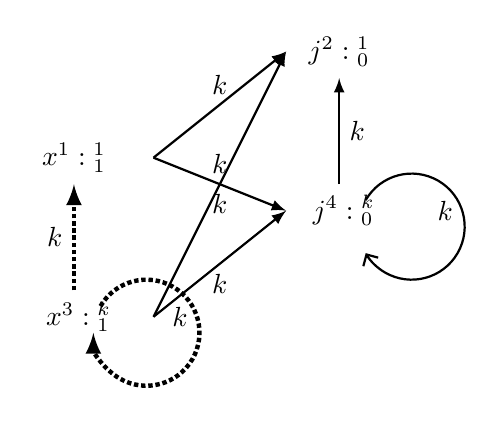
\begin{tikzpicture}[scale=\textwidth/18cm,samples=200]
  \draw[] (0, 7) circle (0pt) node
  {\textbf{$x^1: {}^{1}_{1}$}};
  \draw[] (0, 4) circle (0pt) node
  {{ $x^3: {}^{k}_{1}$}};
  % Counter Variables
  \draw[] (5, 9) circle (0pt) node {{$j^2: {}^{1}_{0}$}};
  \draw[] (5, 6) circle (0pt) node {{ $j^4: {}^{k}_{0}$}};
  %
  % Value Dependency Edges:
  \draw[ ultra thick, -latex, densely dotted,] (0, 4.5)  -- node[left]{\highlight{$k$}} (0, 6.5) ;
  \draw[ ultra thick, -latex, densely dotted,] (0.5, 4.2) arc (150:-180:1);
  \draw[] (2, 4) node []{\highlight{$k$}};
  \draw[ thick, -Straight Barb] (5.5, 6.2) arc (150:-150:1);
  \draw[] (7, 6) node []{\highlight{$k$}};
  \draw[ thick, -latex] (5, 6.5)  -- node[right]{\highlight{$k$}} (5, 8.5) ;
  % Control Dependency
  \draw[ thick,-latex] (1.5, 7)  -- node[above]{\highlight{$k$}} (4, 9) ;
  \draw[ thick,-latex] (1.5, 4)  -- node[above]{\highlight{$k$}} (4, 9) ;
  \draw[ thick,-latex] (1.5, 7)  -- node[below]{\highlight{$k$}} (4, 6) ;
  \draw[ thick,-latex] (1.5, 4)  -- node[below]{\highlight{$k$}} (4, 6) ;
  \end{tikzpicture}
  \caption{}
    \end{centering}
    \end{subfigure}
  }
   \caption{(a) Simple While Loop Example, (b) The Program-Based Dependency Graph generated from $\THESYSTEM$.}
  \label{fig:alg_adaptsearch_simplewhile}
  \end{figure}
  % \begin{figure}
% \centering
% {
% % \footnotesize
% \begin{subfigure}{.25\textwidth}
% \begin{centering}
% $ 
% \begin{array}{l}
%   \kw{whileSim(k)} \triangleq \\
%   \clabel{ \assign{j}{k} }^{0} ; \\
%   \clabel{ \assign{x}{\query(\chi[0])} }^{1} ; \\
%       \ewhile ~ \clabel{j > 0}^{2} ~ \edo ~ \\
%       \Big(
%        \clabel{\assign{x}{\query(\chi[x]) }}^{3}  ; \\
%       \clabel{\assign{j}{j-1}}^{4}       \Big)
%   \end{array}
% $
% \caption{}
% \end{centering}
% \end{subfigure}
% \quad
%   \begin{subfigure}{.6\textwidth}
%   \begin{centering}
%   \begin{tikzpicture}[scale=\textwidth/18cm,samples=200]
% \draw[] (0, 7) circle (0pt) node
% {\textbf{$x^1: {}^{1}_{1}$}};
% \draw[] (0, 4) circle (0pt) node
% {{ $x^3: {}^{k}_{1}$}};
% % Counter Variables
% \draw[] (5, 9) circle (0pt) node {{$j^2: {}^{1}_{0}$}};
% \draw[] (5, 6) circle (0pt) node {{ $j^4: {}^{k}_{0}$}};
% %
% % Value Dependency Edges:
% \draw[ ultra thick, -latex, densely dotted,] (0, 4.5)  -- (0, 6.5) ;
% \draw[ ultra thick, -latex, densely dotted,] (0.5, 4.2) arc (150:-180:1);
% \draw[ thick, -Straight Barb] (5.5, 6.2) arc (150:-150:1);
% \draw[ thick, -latex] (5, 6.5)  -- (5, 8.5) ;
% % Control Dependency
% \draw[ thick,-latex] (1.5, 7)  -- (4, 9) ;
% \draw[ thick,-latex] (1.5, 4)  -- (4, 9) ;
% \draw[ thick,-latex] (1.5, 7)  -- (4, 6) ;
% \draw[ thick,-latex] (1.5, 4)  -- (4, 6) ;
% \end{tikzpicture}
% \caption{}
%   \end{centering}
%   \end{subfigure}
% }
% % \end{wrapfigure}
% % \end{equation*}
% \vspace{-0.4cm}
%  \caption{(a) Simple While Loop Example, (b) The Program-Based Dependency Graph generated from $\THESYSTEM$.}
% \label{fig:alg_adaptsearch_simplewhile}
% \vspace{-0.5cm}
% \end{figure}
% Analysis Results: $ \progA(\kw{whileRec}(k)) = 1 + k$
%
If we traverse on the program-based dependency graph, and decrease the weight of $x^3$ (the weight $k$ is symbolic) by one after every visit,
% We can simply adopt either a deep first strategy to estimate the adaptivity as the length of the longest weight path, as 
% in Algorithm~\ref{alg:overadp_alg}.
we will never terminate because we only know $k \in \mathbb{N}$.

To solve this non-termination challenge, we switch to another walk finding approach: we first find a  longest path in the program-based dependency graph and then approximate the walk with the path.
Through a simple deep first search algorithm, we find the longest weighted path as the dotted arrow in Figure~\ref{fig:alg_adaptsearch_simplewhile},
$x^3: {}^k_1 \to x^1: {}^1_1 $.
Then, by summing up the weights on this path where the vertices has query annotation $1$, deep first search algorithm gives the adaptivity bound $1 + k$.
This is a the tight bound for this program's adaptivity.
% Look at the two-round example in overview, 
% it is easy to find that the longest weighted path is  $x^3 : {}^{k}_{1} \to a^5 : {}^{k}_{0} \to l^6 : {}^{1}_{0}$ with weighted query length $1 + k$.
% If we use this path to approximate a finite walk, and weight of each vertex as
% %  their visiting times, 
% its visiting time,
% then it isn't a qualified walk. 
% In the approximated walk, we have the vertices as $x^3 \to \cdots \to x^3 \to a^5 \to \cdots \to a^5 \to l^6$.

% However, this gives us over-approximation to a large extend in other cases as in \textbf{Approximation Challenge}.
% In Algorithm~\ref{alg:adpt_alg}, 
% we first find all the strong connected components of this graph, 
\textbf{Approximation Challenge:}
% As in Definition~\ref{def:finitewalk}, w
When we adopt a deep first strategy to search for the longest weighted path, and then use the path to approximate the adaptivity. We find that this gives us over-approximation to a large extend.
% Specifically, according to the finite walk definition in Definition~\ref{def:finitewalk},
% the visiting time of every vertex on a walk should be no more than its weight.
% However, by searching for the longest weighted path, 
% % and approximating the finite walk by this weight path, 
% and use it as the approximated finite walk with the longest query length, 
% the visiting times of the vertex on 
% % it 
% this approximated walk could 
% % possibly 
% exceed 
% % its weights. 
% the visiting times it can have.
% Then, this approximated walk isn't a qualified walk by Definition~\ref{def:finitewalk}, 
% and the weighted query length of this path is obviously greater than the maximum query length of the finite walk.
This over-approximation could result in a $\infty$ adaptivity upper bound on the program with actual adaptivity $2$.
Look at the two-round example in overview, 
it is easy to find that the longest weighted path is  $x^3 : {}^{k}_{1} \to a^5 : {}^{k}_{0} \to l^6 : {}^{1}_{0}$ with weighted query length $1 + k$.
If we use this path to approximate a finite walk, and weight of each vertex as
%  their visiting times, 
its visiting time,
then it isn't a qualified walk. 
In the approximated walk, we have the vertices as $x^3 \to \cdots \to x^3 \to a^5 \to \cdots \to a^5 \to l^6$.
Because $l^6$ can only be visited as most once by its weight,
% and this lead to 
resulting in the restriction on the maximum visiting time of $x^3$,
such that $x^3$ is only able to be visited at most once as well.
%
However, $x^3$ is visited $k$ times in this approximated walk.
% Moever, with the longest query length, then 
In order to have $x^3$ be visited $k$ time, we need to go back to 
$x^3$ on this walk from either $a^5$ or $l^6$ for $k$ time.
This is impossible since there is no edge going back to $x^3$ in $\progG(twoRound)$.
Obviously,
% the with the weighted length $1 + k$. It is obviously
its weighted query length, $1 + k$, 
% which is 
over approximates 
% its 
the adaptivity of this example to a large extend, which supposed to be $2$. 
%  for this program, 
% that 


These challenges motivate us to design a walk search algorithm through a combination of 
% DFS and BFS algorithm 
deep first search and breath first search strategy. 
% \wq{
This walk search algorithm consists of two components:
the path searching algorithm, $\pathsearch$ (in Algorithm~\ref{alg:adpt_alg})
which search for a 'suitable' path relying on the strong connected components of the program based dependency graph, 
and $\kw{\pathsearch_{scc}(G)}$ (in Algorithm~\ref{alg:adaptscc}) which approximates the
path.
% path found by Algorithm~\ref{alg:adpt_alg} 
% to a precise walk on the SCC
% and computes the adaptivity.
% These challenges give us the necessary to design a walk search algorithm through a combination of 
% % DFS and BFS algorithm 
% deep first search and breath first search strategy
% % as defined 
% as in Algorithm~\ref{alg:adpt_alg} and Algorithm~\ref{alg:adaptscc}.
%
The $\pathsearch$ as shown in Appendix Algorithm~I, takes our program-based dependency graph as input, and outputs the estimated adaptivity by two steps. 1. Process the input graph to a simplified graph 2. Perform
     the standard breath first search strategy to find the longest weighted path on this simplified graph and return the length as adaptivity.
The step 2 is not interesting, we now discuss step 1. 
The input dependency graph may contain circle due to the while loop, we simplify (shrank) the input graph by replacing every strong connected components(circle) of the graph with, the vertex whose weight is the adaptivity of the SCC 
(a subgraph of the input one) calculated by the $\pathsearch_{\kw{scc}}$. 
The SCC is found by using the Kosaraju's algorithm.
% \wq{cite}. 
The details of this algorithm is explained as follows.
    % This algorithm first finds all the strong connected components (SCC) of $\progG(c)$ using the Kosaraju’s algorithm in line:3. 
    % Every $\kw{SCC_1}, \cdots, \kw{SCC_n}$
    % where $0 \leq n \leq |\vertxs|$ is a sub-graph of $\progG(c)$, where $\kw{SCC_i} = (\vertxs_i, \edges_i, \weights_i, \qflag_i)$.
    % % where $\kw{SCC_i} = (\vertxs_i, \edges_i, \weights_i, \qflag_i)$.
    % Then, 
    % % we compute the adaptivity on every SCC, which is a subgraph of the $\progG(c)$, in line:4-5 by Algorithm~\ref{alg:adaptscc}.
    % it computes the adaptivity on every SCC
    % % , which is a subgraph of the $\progG(c)$, 
    % in line:4-5 by Algorithm~\ref{alg:adaptscc}.
    % % We guarantee the soundness of the adaptivity on SCC by Lemma~\ref{lem:sound_adaptalg_scc} with proof 
    % in Appendix.
    % % ~\ref{apdx:adaptalg_soundness}.
    % The $\progG(c)$ is then shrunk into an acyclic directed graph where 
    % % vertices are all the SCCs and edges are between every SCCs with their adaptivities as weights.
    % $\kw{SCC_1}, \cdots, \kw{SCC_n}$ are vertices with their adaptivities as weights.
    % % , and directed edges are .
    % For every $(v_i, v_j) \in \edges$ such that $v_1 \in \vertxs_i$, $v_j \in \vertxs_j$ and $i \neq j$,
    % there is a edge $(s_i, s_j)$ in this shrank graph. \\ 
    % Then, we use the standard breath first search strategy to find the longest weighted path
    % %  w.r.t. all the SCCs and their adaptivities.
    % on this shrank graph and return the length as adaptivity.
    % \\
%     We guarantee that 
%     % this longest weighted path is a sound computation of the adaptivity on this,
%     the length of this longest weighted path is a sound computation of the adaptivity for program $c$,
%     % as well as 
%     and this longest weighted path a sound computation of the finite walk having the longest query length 
%     % on this graph, in Theorem~\ref{thm:sound_adaptalg}
%     on $c$'s program based dependency graph, in Theorem~\ref{thm:sound_adaptalg}
%     in Appendix.
%     % ~\ref{apdx:adaptalg_soundness}.
% %    
% % \todo{add proof} 
% We also guarantee the conditional completeness of the adaptivity computation for graphs under the case that 
% $c$'s Program-Based Dependency Graph $\progG(c)$ is acyclic directed
% in Theorem~\ref{thm:adaptalg_pcomplete} 
% in Appendix~\ref{apdx:adaptalg_completeness}.
%
\paragraph*{The Adaptivity Computation Algorithm ($\pathsearch$)}
\begin{algorithm}
    \caption{
    {Adaptivity Computation Algorithm ($\pathsearch$)}
    \label{alg:adpt_alg}
    }
    \begin{algorithmic}[1]
    \REQUIRE $G = (\vertxs, \edges, \weights, \qflag)$ \#\{The program based dependency graph\}
    % with a start vertex $s$ and destination vertex $t$ .
    \STATE  {\bf {$\kw{\pathsearch(G)}$}:}  
    \STATE {\bf init} 
    % \\
    % current node: $c$, 
    \\
    $q$: empty queue.
    % \\
    % $\kw{visited}$: List of length $|\vertxs|$, initialize with $\efalse$.
    % \\
    % $\kw{SSCvisited}$: List of length $|\vertxs|$, initialize with $\efalse$.
    % \\ 
    % $\kw{adapt_{scc}(SCC_i) = \pathsearch_{scc}(SCC_i)}$.
    \\
    $\kw{adapt}$ : the adaptivity of this graph initialize with $0$.
    \\
    \STATE Find all Strong Connected Components (SCC) in $G$: $\kw{SCC_1}, \cdots, \kw{SCC_n}, 0 \leq n \leq |\vertxs|$, 
    % where $\kw{SCC_i} = (\vertxs_i, \edges_i, \weights_i, \qflag_i)$.
    % and assign each vertex $x^i$ with an SCC number $\kw{SCC}(x^i)$
    \STATE {\bf for} every SCC: $\kw{SCC_i}$, compute its Adaptivity $\kw{SCC_i}$:
    \STATE \quad $\kw{adapt_{scc}[SCC_i] = \pathsearch_{scc}(SCC_i)}$;
    \STATE {\bf for} every $\kw{SCC_i}$:
    \STATE \qquad $q.append(\kw{SCC_i})$;
    \STATE \qquad $\kw{adapt_{tmp}} = 0$;
    \STATE \qquad {\bf while} $q$ isn't empty:
    \STATE \qquad \qquad $\kw{s} = q.pop()$;  \#\{take the top SCC from head of queue\}
    \STATE \qquad \qquad  $\kw{adapt_{tmp}}_0= \kw{adapt_{tmp}}$; \#\{record the adaptivity of last level\}
    \STATE \qquad \qquad  $\kw{SCC_{max}}$;  \#\{record the SCC with longest walk in this level\}
    % initialize cycle-adapt = 0.
    \STATE \qquad \qquad {\bf for} every 
    % SCC having a directed edge from $s$ of $s$: $\kw{SCC'}$:
    % directed edge goes out of $\kw{s}$ and connects a 
    different SCC, $\kw{s'}$ connected by $\kw{s}$ by a directed edge from $\kw{s}$:
    % \STATE \qquad \qquad   cycle-adapt$ = \max($cycle-adapt, $\kw{dfs_{refine}(G, v, v)})$;
    % \STATE \qquad \qquad \qquad \#\{compute the adaptivity of vertex $v$  on $\kw{SCC}(v)$, and update r[v] with the SCC-adapt\}
    % \STATE \qquad \qquad \qquad $ r[v] = r[s] + \kw{dfs_{refine}(G, v, visited)})$; 
    \STATE \qquad \qquad \qquad {\bf if} $(\kw{adapt_{tmp}} < \kw{adapt_{tmp}}_0 + \kw{adapt_{scc}[s']})$:
    \STATE \qquad \qquad \qquad \qquad $\kw{adapt_{tmp}} = \kw{adapt_{tmp}}_0 + \kw{adapt_{scc}[s']}$; 
    \STATE \qquad \qquad \qquad \qquad $\kw{SCC_{max} = s'} $; \#\{update the SCC with longest walk in this level\} 
    % \STATE \qquad   $r[c] = r[c] + $cycle-adapt;
    % \STATE \qquad for all unvisited vertex $v$ having directed edge from c and $! \kw{cycle}(c)$:
    % \STATE \qquad \qquad $r[v] = r[c] + \flag(v)$; 
    % \STATE \qquad \qquad \qquad  \#\{mark all the nodes with the same $\kw{SCC}$ number as visited\} 
    % \STATE \qquad \qquad \qquad  \#\{append the unvisited vertex to the rear of the queue\}
    % \STATE \qquad \qquad \qquad  \#\{mark all the nodes with the same $\kw{SCC}$ number as visited\} 
    % \STATE \qquad \qquad for $v \in V$,   $\kw{visited}[s] = 1$;
    \STATE \qquad \qquad \qquad $q.append(\kw{SCC_{max}})$;
    \STATE \qquad $\kw{adapt} = \max(\kw{adapt}, \kw{adapt_{tmp}})$;    
    \RETURN $\kw{adapt}$.
    \end{algorithmic}
    \end{algorithm}
    %
%
    % In Algorithm~\ref{alg:adpt_alg}, 
    % it 
    This algorithm first finds all the strong connected components (SCC) of $\progG(c)$ using the Kosaraju’s algorithm in line:3.
    Every $\kw{SCC_1}, \cdots, \kw{SCC_n}$
    where $0 \leq n \leq |\vertxs|$ is a sub-graph of $\progG(c)$, where $\kw{SCC_i} = (\vertxs_i, \edges_i, \weights_i, \qflag_i)$.
    % where $\kw{SCC_i} = (\vertxs_i, \edges_i, \weights_i, \qflag_i)$.
    Then, 
    % we compute the adaptivity on every SCC, which is a subgraph of the $\progG(c)$, in line:4-5 by Algorithm~\ref{alg:adaptscc}.
    it computes the adaptivity on every SCC
    % , which is a subgraph of the $\progG(c)$, 
    in line:4-5 by Algorithm~\ref{alg:adaptscc}.
    We guarantee the soundness of the adaptivity on SCC by Lemma~\ref{lem:sound_adaptalg_scc} with proof in Appendix~\ref{apdx:adaptalg_soundness}.
    The $\progG(c)$ is then shrunk into an acyclic directed graph where 
    % vertices are all the SCCs and edges are between every SCCs with their adaptivities as weights.
    $\kw{SCC_1}, \cdots, \kw{SCC_n}$ are vertices with their adaptivities as weights.
    % , and directed edges are .
    For every $(v_i, v_j) \in \edges$ such that $v_1 \in \vertxs_i$, $v_j \in \vertxs_j$ and $i \neq j$,
    there is a edge $(s_i, s_j)$ in this shrank graph. \\ 
    Then, we use the standard breath first search strategy to find the longest weighted path
    %  w.r.t. all the SCCs and their adaptivities.
    on this shrank graph and return the length as adaptivity.
    \\
    We guarantee that 
    % this longest weighted path is a sound computation of the adaptivity on this,
    the length of this longest weighted path is a sound computation of the adaptivity for program $c$,
    % as well as 
    and this longest weighted path a sound computation of the finite walk having the longest query length 
    % on this graph, in Theorem~\ref{thm:sound_adaptalg}
    on $c$'s program based dependency graph, in Theorem~\ref{thm:sound_adaptalg}
    in Appendix.
    % ~\ref{apdx:adaptalg_soundness}.
%    
% \todo{add proof} 
We also guarantee the conditional completeness of the adaptivity computation for graphs under the case that 
$c$'s Program-Based Dependency Graph $\progG(c)$ is acyclic directed
in Theorem~\ref{thm:adaptalg_pcomplete} 
in Appendix~\ref{apdx:adaptalg_completeness}.
    % for every vertex which isn't on any SCC, it is easy to know that it will be visited 
    % at most once given no edges going back to this vertex. We can know the adaptivity on the SCC 
     %
    % \begin{algorithm}
    % \caption{
    % {Longest Adaptivity Search Algorithm ($\pathsearch$)}
    % \label{alg:adpt_alg}
    % }
    % \begin{algorithmic}
    % \REQUIRE Weighted Directed Graph $G = (\vertxs, \edges, \weights, \flag)$ with a start vertex $s$ and destination vertex $t$ .
    % \STATE  {\bf {bfs $(G)$}:}  
    % \STATE {\bf init} 
    % \\
    % current node: $c$, 
    % \\
    % queue: $q$ : List, add into $a$ an arbitrary v from $\vertxs$. 
    % \\
    % visited: List of length $|\vertxs|$, initialize with $\efalse$.
    % \\
    % results: $r$ : List of length $|\vertxs|$, initialize with -1.
    % \\
    % curr$\kw{flowcapacity}$: INT, initialize MAXINT.
    % \\
    % querynum: INT, initialize 0. \#\{To count the query numbers when we are walking inside a cycle\}
    % \\
    % \STATE \qquad {\bf while} $q$ isn't empty:
    % \STATE \qquad \qquad take the vertex from head $c= q.pop()$
    % \STATE \qquad \qquad mark $c$ as visited, visited $[c] = 1$.
    % \STATE \qquad \qquad {\bf if} $\kw{cycle}(c)$  \#\{we are inside a cycle\}
    % \STATE \qquad \qquad \qquad curr$\kw{flowcapacity}$ = min($\weights$(c), curr$\kw{flowcapacity}$).
    % \STATE \qquad \qquad \qquad querynum += $\flag(c)$.
    % \STATE \qquad \qquad  \qquad for all unvisited vertex $v$ having directed edge from c:
    % \STATE \qquad \qquad \qquad \qquad r[v] = r[c]; q.add(v)
    % \STATE \qquad \qquad \qquad  {\bf if}  $v$ is visited, then the circle finished
    % \STATE \qquad \qquad \qquad \qquad update the result $r[v] =  \max(r[v], r[c] + $curr$\kw{flowcapacity}$*querynum)
    % \STATE \qquad \qquad \qquad \qquad curr$\kw{flowcapacity}$ = MAXINT
    % \STATE \qquad \qquad \qquad \qquad querynum = 0.  
    % \STATE \qquad \qquad {\bf else} 
    % \STATE \qquad \qquad \qquad for all unvisited vertex $v$ having directed edge from c:
    % \STATE \qquad \qquad \qquad  \qquad $r[v] = \max(r[v], r[c] + \flag(c))$; q.add(v)
    % \RETURN max($r$)
    % \end{algorithmic}
    % \end{algorithm}
    %
%
    % \begin{algorithm}
    %     \caption{
    %     {Over-Approximated Adaptivity on SCC}
    %     \label{alg:overadp_alg}
    %     }
    %     \begin{algorithmic}
    %     \REQUIRE Weighted Directed Graph $G = (\vertxs, \edges, \weights, \qflag)$ with a start vertex $s$ and destination vertex $t$ .
    %     \STATE  {\bf {$\kw{dfs_{naive}(G, c,visited)}$}:}  
    %     % \STATE {\bf init} 
    %     % \\
    %     % current node: $c$, 
    %     % \\
    %     % visited: List of length $|\vertxs|$, initialize with $\efalse$.
    %     % \\
    %     % \STATE {\bf if} $c = s$:
    %     % \RETURN \qquad  $\weights(s)*\flag(s) $.
    %     \STATE $r[c] = \weights(c)*\qflag(c) $
    %     \STATE {\bf for}  all vertex $v$ having directed edge from $c$:
    %     \STATE \qquad {\bf if}  $v$ is unvisited:
    %     \STATE \qquad \qquad  \#\{mark $v$ as visited\} $\kw{visited}[v] = 1$;
    %     \STATE \qquad \qquad $r[c] += \kw{dfs_{naive}(G, v, visited)}$;
    %     % \STATE \qquad {\bf else}: \#\{There is a cycle finished\}
    %     % \RETURN \qquad \qquad $\weights(v)*\flag(v) $.
    %     \RETURN $r[c]$
    %     \end{algorithmic}
    %     \end{algorithm}%
        %
  \paragraph*{Adaptivity Computation Algorithm on SCC Graph ($\kw{\pathsearch_{scc}(G)}$)}
    \begin{algorithm}
            \caption{
            {Adaptivity Computation Algorithm on SCC Graph }
            \label{alg:adaptscc}
            }
            \begin{algorithmic}[1]
              \REQUIRE $G = (\vertxs, \edges, \weights, \qflag)$ \#\{An Strong Connected program based dependency Graph\}
            \STATE  {\bf {$\kw{\pathsearch_{scc}(G)}$}:}  
            \STATE {\bf init} 
            \\
            $\kw{r_{scc}}$: $EXPR(\constdom)$, initialized $0$, the Adaptivity of this SCC
            \STATE \qquad {\bf init} 
            % \STATE \qquad current node: $c$, 
            % \\
            % visited: List of length $|\vertxs|$, initialize with $\efalse$.
            % \\ \qquad  $\kw{r_{scc}}$ : initialize $0$, the adaptivity of this graph
            \\ \qquad  $\kw{visited}$ : $\{0, 1\}$ List, 
            \\ \qquad  \#\{length $|\vertxs|$, initialize with $0$ for every vertex, recording whether a vertex is visted.\}
            \\ \qquad  $\kw{r}$ : $EXPR(\constdom)$ List, 
            \\ \qquad  \#\{length $|\vertxs|$, initialize with $\qflag(v)$ for every vertex, recording the adaptivity reaching each vertex.\}
            \\ \qquad  $\kw{flowcapacity}$: $EXPR(\constdom)$ List, 
            % INT List of length $|\vertxs|$, initialize MAXINT. 
            \\ \qquad  \#\{length $|\vertxs|$, initialize with $\infty$ for every vertex,
            % \#\{For every vertex, 
            recording the minimum weight when the walk reaching 
            that vertex, inside a cycle\}
            \\ \qquad  $\kw{querynum}$: INT List,
            %  of length $|\vertxs|$, initialize with $\qflag(v)$ for every vertex. 
            \\ \qquad  \#\{length $|\vertxs|$, initialize with $\qflag(v)$ for every vertex, 
            % \#\{For every vertex, 
            recording the query numbers when the path reaching 
            that vertex, inside a cycle\}
            \STATE {\bf if} $|\vertxs| = 1$ and $|\edges| = 0$:
            \STATE \qquad {\bf return}  $\qflag(v)$
            \STATE  {\bf def} {$\kw{dfs(G, c,visited)}$}:
            % \STATE \qquad update the length of the longest path reaching this vertex
            % $r[s] =  r[s] + $$\kw{flowcapacity}$[s] * querynum[s].
            % \RETURN  \qquad $r[s]$.      
            \STATE \qquad {\bf for} every vertex $v$ 
            % having directed edge from $c$:
            connected by a directed edge from $c$:
            \STATE \qquad \qquad {\bf if} $\kw{visited}[v] = \efalse$:
            \STATE \qquad \qquad \qquad $\kw{flowcapacity[v] = \min(\weights(v), {flowcapacity}[c])}$;
            \STATE \qquad \qquad \qquad $\kw{querynum[v] = querynum[c] + \qflag(v)}$;
            % \STATE \qquad \qquad \qquad \#\{do not update the length of the longest walk reaching $v$ until the cycle is finished\}
            % \STATE \qquad \qquad \qquad $\kw{r[v] =  r[c] + flowcapacity[v] \times querynum[v]} $; \#\{do not update the length of the longest walk reaching $v$ until the cycle is finished\}
            \STATE \qquad \qquad \qquad $\kw{r[v] =  \max(r[v], flowcapacity[v] \times querynum[v]}) $; 
            % \#\{do not update the length of the longest walk reaching $v$ until the cycle is finished\}
            \STATE \qquad \qquad \qquad  $\kw{visited}[v] = 1$; %\#\{mark $v$ as visited\}
            \STATE \qquad \qquad \qquad $\kw{dfs(G, v, visited)}$;
            \STATE \qquad \qquad {\bf else}: \#\{There is a cycle finished\}
            % \STATE \qquad \qquad \qquad \#\{update the length of the longest path reaching this vertex\}
            \STATE \qquad \qquad \qquad 
            $\kw{r[v] =  \max(r[v], r[c] +  \min(\weights(v), {flowcapacity}[c]) * (querynum[c] + \qflag(v)))}$; \#\{update the length of the longest walk reaching this vertex on this cycle\}
            %  $\kw{r[v] =  \max(r[v], r[c] + flowcapacity[v] * querynum[v])}$; \#\{update the length of the longest walk reaching this vertex on this cycle\}
            %  \STATE \qquad \qquad \qquad \#\{Recover the $\kw{flowcapacity}$ and querynumber to previous state, for different loops\}
            % \STATE \qquad \qquad \qquad $\kw{flowcapacity[v] = flowcapacity[c]}$; \#\{Recover the $\kw{flowcapacity}$\}
            % \STATE \qquad \qquad \qquad $\kw{querynum[v] = querynum[c]}$;\#\{Recover the $\kw{querynum}$\}
            \STATE \qquad {\bf return}  $\kw{r[c]}$
            \STATE  {\bf for} every vertex $v$ in $\vertxs$:
            \STATE  \qquad initialize the $\kw{visited, r, flowcapacity, querynum}$;
            \STATE  \qquad $\kw{r_{scc} = \max(r_{scc}, dfs(G, v, \kw{visited} ))}$ ; 
            \RETURN  $\kw{r_{scc}}$
            \end{algorithmic}
            \end{algorithm}
            % \\
% Following is the challenge of computing the adaptivity on a program based dependency graph.
% In order to search for the finite walk having the longest query length, which isn't a simple longest weighted path.
% \\
% the visiting times of every vertex on this walk should be no more than its weight, which is a symbolic expression.
% So we cannot simply search for the longest weight path where the visiting times of the vertex on it could possibly exceed its weights.
% We can neither simply traverse on this graph by decreasing the weight of every node by 1 after every visiting,
% because the weight is symbolic and simply traversing leads to non-termination.
% \\
% In Algorithm~\ref{alg:adaptscc}, 
This algorithm takes a subgraph of the program-based dependency graph as input, to be precise, the input graph is SCC, and the output is the adaptivity of this SCC. 
For an SCC containing only one vertex without any edge, it returns the query annotation of this vertex as adaptivity.
For SCC containing at least one edge, 
There are three steps in this algorithm: 1. find out all the paths in the input SCC 2. Calculate the adaptivity of every path using our designed adaptivity counting method. 3. Return the maximal adaptivity among all the paths. The step 3 is trivial. Because our input graph is SCC, when we start traversing from a vertex, we will finally go back to this vertex. The paths we find in step 1 are all those with the same starting and ending vertex. The most interesting part is step 2. 
We discuss as follows.

This algorithm first check if an SCC contains only one vertex without any edge, as in line:4-5 in Algorithm~\ref{alg:adaptscc}.
% then 
% \\
% If yes, then it's easy to know that it will be visited 
% at most once since there isn't edge going back to this vertex. 
% So we can know that the adaptivity on this SCC is at most one if it is a query vertex,
% and zero otherwise.
% \\
% If not, then 
Again, for 
the SCC containing only one vertex without any edge, as in line:4-5 in Algorithm~\ref{alg:adaptscc}.
% then 
% If yes, then i
% it's easy to know that it will be visited 
% at most once since there isn't edge going back to this vertex. 
% So we can know 
The adaptivity on this SCC is at most one if it is a query vertex,
and zero otherwise.
$\kw{\pathsearch_{scc}(G)}$ return query annotation directly as in line:4-5.
% So $\kw{\pathsearch_{scc}(G)}$ return query annotation directly as in line:4-5.
\\
% For the SCC contains at least one edge, we are searching for the finite walk having the longest query length through a deep first search strategy.
For the SCC containing at least one edge, 
we compute the adaptivity for each path 
on the fly of searching for the paths 
in the
% design a 
recursion algorithm $\kw{dfs}$ designed based on 
a deep first search strategy 
% of this algorithm is described as follows,
from line: 6-16 in $\kw{\pathsearch_{scc}(G)}$ in Algorithm~\ref{alg:adaptscc}.
\\
% The difficulty is, the visiting times of every vertex on this walk should be no more than its weight, which is a symbolic expression.
% As the two challenges discussed above, we want to guarantee the visiting time of each vertex smaller than 
% its weight, in the meantime the algorithm termination. 
% Additionally, we are computing the query length rather than sum of the weights.
% We design a deep first search strategy
% % of this algorithm is described as follows,
% from line: 6-16 in Algorithm~\ref{alg:adaptscc}, 
% searching for the finite walk having the longest query length
% %  through a deep first search strategy
% with a capacity limitation and use special parameter to compute the adaptivity.
%
As the \textbf{Approximation Challenge} discussed above, 
we want to guarantee the visiting time of each vertex smaller than 
its weight and compute the adaptivity accurately, in the meantime guarantee the algorithm termination. 
It uses a capacity limitation and  special parameters to achieve it,
specifically as follows.
Additionally, we are computing the query length rather than sum of the weights.
We design a deep first search strategy
% of this algorithm is described as follows,
from line: 6-16 in Algorithm~\ref{alg:adaptscc}, 
% searching for the finite walk having the longest query length
%  through a deep first search strategy
with a capacity limitation and use special parameter to compute the adaptivity.
% for every path.
%
% for every path.
% So we cannot simply search for the longest weight path where the visiting times of the vertex on it could possibly exceed its weights.
% We can neither simply traverse on this graph by decreasing the weight of every node by 1 after every visiting,
% because the weight is symbolic and simply traversing leads to non-termination.
% \\
\\
In order to
guarantee the termination, 
% this algorithm 
$\kw{\pathsearch_{scc}(G)}$
terminates the recursion if monitored a cycle, as in line:8 and line:14, through a boolean list $\kw{visited}$.
This guaranteed the termination and solved the \textbf{Challenge II.} discussed above.
% \todo{solve the challenge 2} 
% search for finite walk  
% So we use the dfs to search for the 
\\
% In order to
% solve the \textbf{Challenge I},
% specifically guarantee the visiting times of each vertex by its weight, 
% we use a special parameter $\kw{flowcapacity}$  to track the minimum weight during the 
% % dfs process, 
% deep first searching along the walk, 
% also a parameter $\kw{querynum}$
% % to compute the query length of this walk
% to track the total number of vertices which are query vertices along the walk in order to compute the query length of this walk.
In order to
solve the \textbf{Approximation Challenge},
specifically guarantee the visiting times of each vertex by its weight
and compute the adaptivity accurately, 
we use a special parameter $\kw{flowcapacity}$  to track the minimum weight
along the path during the 
% dfs process, 
% deep first 
searching procedure, 
and a parameter $\kw{querynum}$
% to compute the query length of this walk
to track the total number of vertices with query annotation $1$
% which are query vertices 
along the path 
in order to compute the query length.
% 
% \todo{solve the challenge 1, specifically in the dfs strategy
% of this algorithm is described as follows,
% from line: 6-16 in Algorithm~\ref{alg:adaptscc}. } 
% \\
% Then, to compute the query length of this walk, 
% we use another parameter $\kw{querynum}$
% to track the total number of vertices which are query vertices along the walk.

The detail steps of this dfs strategy
% of this algorithm is described as follows,
from line: 3-16 in Algorithm~\ref{alg:adaptscc},
particularly from line: 7-15 on how to 
use these two special parameters to resolve \textbf{Approximation Challenge}
 is described as follows.
 %
 $\kw{flowcapacity}$ is a list of symbolic expressions for every vertex, recording the minimum weight when the path reaches that vertex, which is initialized by $\infty$.
% , inside a cycle\}

$\kw{querynum}$ is a list of integer with length $|\vertxs|$, which is initialized with $\qflag(v)$ for every vertex. 
For every vertex, 
% recording the query numbers when the path reaching.
% in order to 
it records the total query numbers when the path reaching this vertex.

We maintain the minimum weight for the 
$\kw{flowcapacity}$, 
number of query vertices 
$\kw{querynum}$ 
and update the adaptivity for this path $\kw{r}$
alone the path and update the adaptivity reaching 
this vertex, 
when traversing on this graph, as in Algorithm~\ref{alg:adaptscc} from line: 8-13.
% and then recursively dfs on all vertices heading out from this vertex.
% \\
At line: 15 where this vertex is visited, i.e., this path 
going back to its starting node,
we only update the adaptivity $\kw{r}$ reaching this vertex.
% and neither recursion nor update the $\kw{flowcapacity}$  and 
% $\kw{querynum}$.
\\
% Again, Non-recursion in the second branch
% % in order to 
% guarantees the termination and resolves \textbf{Non-Termination Challenge}.
% \\
The updating operations
during the traversing 
(in line: 11) and 
at the end of the traverse (in line: 15),
% in these two branches, 
specifically the $\kw{flowcapacity[v] \times querynum[v]}$ 
% in line: 11 and line: 15 
computes the query length for this path. 
it guarantees 
the visiting times of each vertex on the path reaching a vertex $v$ is no more than 
the maximum visiting it can be on a qualified walk, through $\kw{flowcapacity[v]}$,
and in the same time  compute the query length instead of weighted length accurately through 
$\kw{ querynum[v]}$.
%  its minimum visiting time, 
In this way, we resolve the \textbf{Approximation Challenge} and in the same time without losing the soundness,
% searching for the finite walk having the longest query length through a deep first search strategy
% with a capacity limitation and use special parameter to compute the adaptivity
% for every path.
\\
We first initialize some parameters:
\\
$\kw{visited}$ is initialized as a list of $0$ for every vertex on this SCC, in order to guarantee the termination;
\\ 
$\kw{r}$ is initialized  as a list of integer with length $|\vertxs|$, initialize with $\qflag(v)$ for every vertex. The adaptivity reaching each vertex.
\\ 
$\kw{flowcapacity}$ a list of symbolic expressions for every vertex, recording the minimum weight when the walk reaching that vertex, which  is initialized by $\infty$.
% , inside a cycle\}
\\ 
$\kw{querynum}$ is a list of integer with length $|\vertxs|$, which is initialized with $\qflag(v)$ for every vertex. 
For every vertex, 
% recording the query numbers when the path reaching.
in order to record the total query numbers when the walk reaches a vertex.
\\
Then from line: 5-11, we record the minimum weight and number of query vertices alone the path and update the adaptivity reaching 
this vertex, and then recursively dfs on all vertices heading out from this vertex.
\\
At line: 12 where this vertex is visited, 
we only update the adaptivity reaching this vertex and neither recursion nor update the $\kw{flowcapacity}$  and 
$\kw{querynum}$.
% \\
% Again, Non-recursion in the second branch
% % in order to 
% guarantees the termination and resolves \textbf{Challenge I}.
\\
The updating operation in these two branches, 
specifically $\kw{flowcapacity[v] \times querynum[v]}$ in line: 11 and line: 15 
guarantees 
1.the visiting times of each vertex on the walk reaching $v$ is no more than 
the maximum visiting it can be on this walk, through $\kw{flowcapacity[v]}$. 
%  its minimum visiting time, 
In this way, we resolve the \textbf{Approximation Challenge}  and in the same time without losing the soundness 
% this 
% 2. then 
by using $\kw{flowcapacity[v] \times querynum[v]}$ to compute the query length. 
% without lose the adaptivity.
%
\\
Notice here, another special operation we have in the second branch is Non-updating of
% Non-updating the 
$\kw{querynum}$ and $\kw{flowcapacity}$.
This guarantees both the accuracy and the soundness, formally in Lemma~\ref{thm:sound_adaptalg} in Appendix~\ref{apdx:adaptalg_soundness}.

Now, we show an example illustrating how our two updating operations for adaptivity 
for each path can guarantee both the accuracy and the soundness. 
Look at a Nested While Loop example program in Figure~\ref{fig:alg_adaptsearch_nestedwhile}.
% Notice here, another special operation we have in the second branch is Non-updating of
% % Non-updating the 
% $\kw{querynum}$ and $\kw{flowcapacity}$.
% This guarantees both the accuracy and the soundness.
% Specifically,
% % because a second visiting of the same vertex 
% if this vertex is visited, it indicates that a cycle is monitored and  
% % indicates there is a cycle goes back to this vertex, 
% the traversing on this cycle is finished by going back to this vertex.
% %
% % then, when 
% When we continuously search for walks heading out of this vertex, 
% the minimum weight on this cycle does not affect the walks going out of this vertex that not pass this cycle.
% However, if we keep recording the minimum weight, then we
% %  are restricting 
% restrict the visiting times of vertices on a walk by
%  using the minimum weight of vertices not on this walk.
% %  , it is unsound anymore.
% Then, it is obviously that this leads to unsoundness.
% \todo{example} 
% To under stand how the two operations 
We first search for a path: $y^6 \to y^6$, and compute the adaptivity for this path as 
$k$.
Notice here, another special operation we have in the second branch is Non-updating of
% Non-updating the 
$\kw{querynum}$ and $\kw{flowcapacity}$.
This guarantees both the accuracy and the soundness.
Specifically,
% because a second visiting of the same vertex 
if this vertex is visited, it indicates that a cycle is monitored and  
% indicates there is a cycle goes back to this vertex, 
the traversing on this cycle is finished by going back to this vertex.
%
% then, when 
When we continuously search for walks heading out of this vertex, 
the minimum weight on this cycle does not affect the walks going out of this vertex that not pass this cycle.
However, if we keep recording the minimum weight, then we
%  are restricting 
restrict the visiting times of vertices on a walk by
using the minimum weight of vertices not on this walk.
%  , it is unsound anymore.
Then, it is obviously that this leads to unsoundness.
If we update the $\kw{flowcapacity}[y^6]$ as $k$ after visiting $y^6$ the second time 
on this walk,
% the walk $y^6 \to y^6$,
and continuously visit $x^9$,
then the $\kw{flowcapacity[k]}$ is 
updated as $\min(k, k^2)$.
So
%  which 
% restricting 
the visiting times of $x^9$ is restricted by $k$ on the walk $y^6 \to y^6 \to x^9$.
This restriction excludes the finite walk $y^6 \to y^6 \to x^9 \to x^9$ where $y^6$ and $x^9$ visited by $k^2$ times
in the computation. 
However, the finite walk $y^6 \to y^6 \to x^9 \to x^9$ where $y^6$ is visited $k$ times and $x^9$ $k^2$ times is 
a qualified walk, and exactly the longest walk we aim to find. So, by Non-updating the $\kw{flowcapacity}$ after 
visiting $y$ again, we guarantee that the visiting times og vertices on every searched walk will not be restricted by weights not on this walk,
i.e., the soundness.
\\
In the last line of this dfs algorithm, line: 16, it returns the adaptivity heading out from its input vertex.
\\
By applying this deep first search strategy on every vertex on this SCC, 
we compute the adaptivity of this SCC by taking the maximum 
% adaptivity reaching every vertex on this SCC.
value over every vertex.
%
The soundness is formally guaranteed in Lemma~\ref{lem:sound_adaptalg_scc} in Appendix~\ref{apdx:adaptalg_soundness}.

% Look at a Nested While Loop example program in Figure~\ref{fig:alg_adaptsearch_nestedwhile}.

% Specifically,
% % because a second visiting of the same vertex 
% if this vertex is visited, it indicates that a cycle is monitored and  
% % indicates there is a cycle goes back to this vertex, 
% the traversing on this cycle is finished by going back to this vertex.
% %
% % then, when 
% When we continuously search for walks heading out of this vertex, 
% the minimum weight on this cycle does not affect the walks going out of this vertex that not pass this cycle.
% However, if we keep recording the minimum weight, then we
% %  are restricting 
% restrict the visiting times of vertices on a walk by
%  using the minimum weight of vertices not on this walk.
% %  , it is unsound anymore.
% Then, it is obviously that this leads to unsoundness.
 %
  %
  \begin{figure}
    \centering
    {\footnotesize
    \begin{subfigure}{.4\textwidth}
    \begin{centering}
    % 
    $ 
    \begin{array}{l}
      \kw{nestedWhileMultiVarRecAcross}(k) \triangleq \\
      \clabel{\assign{i}{k} }^{0} ; \\
      \clabel{ \assign{x}{\query(\chi[0])}}^{1} ; \\
      \clabel{ \assign{y}{\query(\chi[1])}}^{2} ; \\
          \ewhile ~ \clabel{i > 0}^{3} ~ \edo ~ \\
          \Big(
           \clabel{\assign{i}{i-1}}^{4} ;\\
           \clabel{\assign{j}{k}}^{5} ;\\
           \clabel{\assign{y}{\query(\chi(\ln(x) + y))} }^{6}  ; \\
           \ewhile ~ \clabel{j > 0}^{7} ~ \edo ~ \\
           \Big(
            \clabel{\assign{j}{j-1}}^{8};\\
            \clabel{\assign{x}{\query(\chi(\ln(y))+\chi[x])} }^{9}
            \Big) \Big)
      \end{array}
    %       
    $
    \caption{}
    \end{centering}
    \end{subfigure}
    \quad
    \begin{subfigure}{.52\textwidth}
      \begin{centering}
      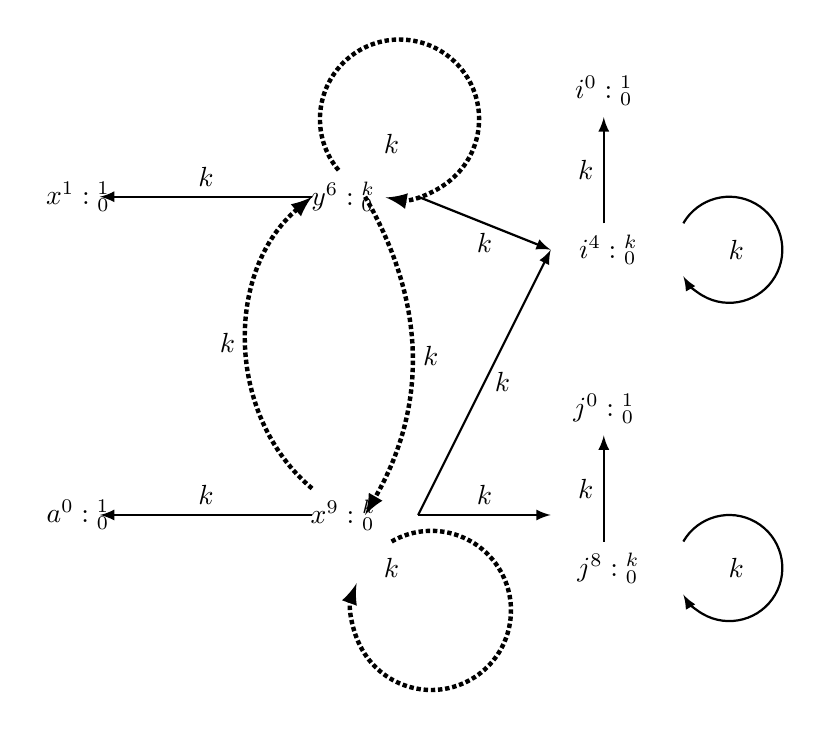
\begin{tikzpicture}[scale=\textwidth/18cm,samples=200]
      % Variables Initialization
      \draw[] (-5, 1) circle (0pt) node{{ $a^0: {}^1_{0}$}};
      \draw[] (-5, 7) circle (0pt) node{{ $x^1: {}^{1}_{0}$}};
      % Variables Inside the Loop
      \draw[] (0, 7) circle (0pt) node{{ $y^6: {}^{k}_{0}$}};
      \draw[] (0, 1) circle (0pt) node{{ $x^9: {}^{k}_{0}$}};
      % Counter Variables
      \draw[] (5, 9) circle (0pt) node {{$i^0: {}^{1}_{0}$}};
      \draw[] (5, 6) circle (0pt) node {{ $i^4: {}^{k}_{0}$}};
      \draw[] (5, 3) circle (0pt) node {{$j^0: {}^{1}_{0}$}};
      \draw[] (5, 0) circle (0pt) node {{ $j^8: {}^{k}_{0}$}};
      % Value Dependency Edges:
      \draw[ ultra thick, -latex, densely dotted,] (0, 7.5) arc (220:-100:1.5);
      \draw[] (1, 8) node [] {\highlight{$k$}};
      \draw[ thick, -latex] (5, 6.5)  -- node[left]{\highlight{{$k$}}}(5, 8.5) ;
      \draw[ thick, -latex] (5, 0.5)  -- node[left]{\highlight{{$k$}}}(5, 2.5) ;
      \draw[ ultra thick, -latex, densely dotted,] (1., 0.5) arc (120:-200:1.5);
      \draw[] (1, 0) node [] {\highlight{$k$}};
      % Value Dependency Edges on Initial Values:
      \draw[ thick, -latex,] (-0.5, 1)  -- node[above]{\highlight{{$k$}}}(-4.5, 1) ;
      \draw[ thick, -latex,] (-0.5, 7)  -- node[above]{\highlight{{$k$}}}(-4.5, 7) ;
      %
      \draw[ ultra thick, -latex, densely dotted,] (-0.5, 1.5)  to  [out=-220,in=220]  
      node[left]{\highlight{{$k$}}}(-0.5, 7);
      \draw[ ultra thick, -latex, densely dotted,]  (0.5, 7) to  [out=-60,in=60] 
      node[right]{\highlight{{$k$}}}(0.5, 1) ;
      % Control Dependency
      \draw[ thick, -latex, ] (6.5, 6.5) arc (150:-150:1);
      \draw[] (7.5, 6) node [] {\highlight{$k$}};
      \draw[ thick, -latex, ] (6.5, 0.5) arc (150:-150:1);
      \draw[] (7.5, 0) node [] {\highlight{$k$}};
      \draw[ thick,-latex] (1.5, 7)  -- node[below]{\highlight{{$k$}}}(4, 6) ;
      \draw[ thick,-latex] (1.5, 1)  -- node[right]{\highlight{{$k$}}}(4, 6) ;
      \draw[ thick,-latex] (1.5, 1)  -- node[above]{\highlight{{$k$}}}(4, 1) ;
   \end{tikzpicture}
   \caption{}
      \end{centering}
      \end{subfigure}
    }
     \caption{(a) Nested While Loop Example, (b) Execution-Based Dependency Graph, (c) The Static Program-Based Dependency graph.}
    \label{fig:alg_adaptsearch_nestedwhile}
    \vspace{-0.5cm}
    \end{figure}
    %
%     When we searched for a walk: $y^6 \to y^6$,
%   if we update the $\kw{flowcapacity}[y^6]$ as $k$ after visiting $y^6$ the second time 
%   on this walk,
%   % the walk $y^6 \to y^6$,
%   and continuously visit $x^9$,
%   then the $\kw{flowcapacity[k]}$ is 
%   updated as $\min(k, k^2)$.
%   So
%   %  which 
%   % restricting 
%   the visiting times of $x^9$ is restricted by $k$ on the walk $y^6 \to y^6 \to x^9$.
%   This restriction excludes the finite walk $y^6 \to y^6 \to x^9 \to x^9$ where $y^6$ and $x^9$ visited by $k^2$ times
%   in the computation. 
%   However, the finite walk $y^6 \to y^6 \to x^9 \to x^9$ where $y^6$ is visited $k$ times and $x^9$ $k^2$ times is 
%   a qualified walk, and exactly the longest walk we aim to find. So, by Non-updating the $\kw{flowcapacity}$ after 
%   visiting $y$ again, we guarantee that the visiting times og vertices on every searched walk will not be restricted by weights not on this walk,
%   i.e., the soundness.
%  \\
% In the last line of this dfs algorithm, line: 16, it returns the adaptivity heading out from its input vertex.
% \\
% By applying this deep first search strategy on every vertex on this SCC, 
% we compute the adaptivity of this SCC by taking the maximum 
% % adaptivity reaching every vertex on this SCC.
% value over every vertex.
% %
% The soundness is formally guaranteed in Lemma~\ref{lem:sound_adaptalg_scc} in Appendix~\ref{apdx:adaptalg_soundness}.
            % \begin{algorithm}
        % \caption{
        % {Refined Adaptivity on $\kw{SCC}$}
        % \label{alg:dfscycle_alg}
        % }
        % \begin{algorithmic}
        % \REQUIRE Weighted Directed Graph $G = (\vertxs, \edges, \weights, \qflag)$ with a start vertex $s$ and destination vertex $t$ .
        % \STATE  {\bf {$\kw{dfs_{refine}(G, c, visited)}$}:}  
        % \STATE {\bf init} 
        % \\
        % current node: $c$, 
        % % \\
        % % visited: List of length $|\vertxs|$, initialize with $\efalse$.
        % \\
        % results: $r$ : INT List of length $|\vertxs|$, initialize with $\qflag(v)$ for every vertex.
        % \\
        % $\kw{flowcapacity}$: INT List of length $|\vertxs|$, initialize MAXINT. 
        % \#\{For every vertex, recording the minimum weight when the walk reaching 
        % that vertex, inside a cycle\}
        % \\
        % querynum: INT List of length $|\vertxs|$, initialize with $\qflag(v)$ for every vertex. 
        % \#\{For every vertex, recording the query numbers when the walk reaching 
        % that vertex, inside a cycle\}
        % \\
        % % \STATE {\bf if} $c = s$:
        % % \STATE \qquad update the length of the longest path reaching this vertex
        % % $r[s] =  r[s] + $$\kw{flowcapacity}$[s] * querynum[s].
        % % \RETURN  \qquad $r[s]$.      
        % \STATE {\bf for}  all vertex $v$ having directed edge from $c$:
        % \STATE \qquad \qquad $\kw{flowcapacity}$[v] = min($\weights(v)$, $\kw{flowcapacity}$[c]);
        % \STATE \qquad \qquad querynum[v] = querynum[c] + $\qflag(v)$;
        % \STATE \qquad \qquad \#\{do not update the length of the longest walk reaching $v$ until the cycle is finished\}
        % \STATE \qquad \qquad $r[v] =  r[c] $;
        % \STATE \qquad {\bf if}  $v$ is unvisited:
        % \STATE \qquad \qquad \#\{mark $v$ as visited\} $\kw{visited}[v] = 1$;
        % \STATE \qquad \qquad $\kw{dfs_{refine}(G, v, visited)}$;
        % \STATE \qquad {\bf else}: \#\{There is a cycle finished\}
        % \STATE \qquad \qquad \#\{update the length of the longest path reaching this vertex\}
        % \STATE \qquad \qquad 
        %  $r[v] =  \max(r[v], r[c] + $$\kw{flowcapacity}$[v] * querynum[v]);
        %  \STATE \qquad \qquad \#\{Recover the $\kw{flowcapacity}$ and querynumber to previous state, for different loops\}
        %  \STATE \qquad \qquad $\kw{flowcapacity}$[v] = $\kw{flowcapacity}$[c];
        %  \STATE \qquad \qquad querynum[v] = querynum[c];
        % \RETURN  $r[c]$
        % \end{algorithmic}
        % \end{algorithm}
        % %
        \begin{algorithm}
          \caption{
          {Over-Approximated Adaptivity on SCC}
          \label{alg:overadp_alg}
          }
          \begin{algorithmic}[1]
          \REQUIRE $G = (\vertxs, \edges, \weights, \qflag)$ \#\{An Strong Connected Symbolic Weighted Directed Graph\}
          % with a start vertex $s$ and destination vertex $t$ .
          \STATE {\bf {$\kw{\pathsearch_{scc-naive}(G)}$}:}  
          \STATE {\bf init} 
          \\
          $\kw{r_{scc}}$: the Adaptivity of this SCC
          % \STATE  {\bf def} {$\kw{dfs_{naive}(G, c,visited)}$}: 
          % % \STATE {\bf init} 
          % % \\
          % % current node: $c$, 
          % % \\
          % % visited: List of length $|\vertxs|$, initialize with $\efalse$.
          % % \\
          % % \STATE {\bf if} $c = s$:
          % % \RETURN \qquad  $\weights(s)*\flag(s) $.
          % \STATE \qquad $r[c] = \weights(c)*\qflag(c) $
          % \STATE \qquad {\bf for}  all vertex $v$ having directed edge from $c$:
          % \STATE \qquad \qquad {\bf if}  $v$ is unvisited:
          % \STATE \qquad \qquad \qquad  \#\{mark $v$ as visited\} $\kw{visited}[v] = 1$;
          % \STATE \qquad \qquad \qquad $r[c] += \kw{dfs_{naive}(G, v, visited)}$;
          % \STATE \qquad {\bf else}: \#\{There is a cycle finished\}
          % \RETURN \qquad \qquad $\weights(v)*\flag(v) $.
          \STATE  {\bf for} every vertex $v$ in $\vertxs$:
          % \STATE  \qquad initialize \kw{visited} with $\efalse$.
          \STATE  \qquad $r_{scc} += \weights(v)*\qflag(v)$  
          \RETURN $r[c]$
          \end{algorithmic}
          \end{algorithm}
          %
\begin{thm}[Soundness of $\pathsearch$]
    \label{thm:sound_adaptalg}
    For every program $c$, given its \emph{Program-Based Dependency Graph} $\progG$,
     $$\pathsearch(\progG) \geq \progA(\progG).$$
\end{thm}




\subsection{Estimated Adaptivity through An Example}
\label{subsec:static-examples}
% Through an advanced adaptive data analysis algorithm - multiple rounds algorithm, 
as in Figure~\ref{fig:multi_graphs}(a) in Example~\ref*{ex:multiplerounds}, I will illustrate how \THESYSTEM gives
the estimated adaptivity for programs.
\begin{example}[Multiple Rounds Algorithm]
\label{ex:multiplerounds}
%
% number of iterations and the distribution sampling primitive $c$.
It takes the user input $k$ which decides the 
number of iterations.
% and the distribution sampling primitive $c$.
It starts from an initialized empty tracking list $I$,
% a score called Nscore $ns=0$ , another score Cscore $cs=0$. There is a hidden database $X$ as well.
% It goes $k$ rounds and every round, the two scores $ns$ and $cs$ are updated by a query result. 
% Then the list $I$ is updated by the two scores for every round. After the $r$ rounds, the algorithm returns the columns of the hidden database $X$ not specified in the tracking list $I$, which is $X\setminus I$. 
{ goes $k$ rounds and at every round, tracking list $I$ is updated by a query result of $\query(\chi[I])$.
% Then the list $I$ is updated by the two scores for every round. 
After $r$ rounds, the algorithm returns the columns of the hidden database $D$ not specified in the tracking list $I$.
% The $\mathrel{\mathsf{update}} ( {I}, (a, p))$ function takes $I, a, p$ as input and compute the updated results for $I$.
% $\mathsf{update}$ function is used here to simplify the complex update computation of Nscore, Cscore and the tracking list $I$.
I use functions $\kw{updnscore}(p,a)$,
$\kw{updcscore}(p,a)$,$\kw{update}(I,ns,cs)$ to simplify the complex update computations of $Nscore$, $Cscore$ and the tracking list $I$, 
which will not affect our analysis.%
}

{The interesting part here is the query asked in each iteration is not independent any more. 
The query in one iteration $j$ now depends on the tracking list $I$ from its previous iteration $j-1$, which is updated by the query result in the same iteration $j-1$. The connection between queries from different iterations, 
 which means these queries are adaptively chosen according to our discussion in overview.
}
% in comparison with the two rounds one, is that the query asked in each iteration is not independent(non-adaptive) anymore.
% For example, the query $q^{j}$ at iteration $j$ now may depend on the tracking list $I$, which comes from the previous iteration $j-1$. Additionally, this list $I$ at iteration $j-1$ is updated by the query result $q^{j-1}$ at the same iteration. Intuitively, I can see the connection between queries from different iterations, which means these queries are adaptively chosen according to our Theorem~\ref{thm:gaussiannoise2}.
The program-based dependency graph is presented 
in Figure~\ref{fig:multi_graphs}(b). 
Its execution-based dependency graph has the same graph, except different weight, so I do not show it again. I can simply replaces $k$ with a function $w_k$ which takes a trace and returns the value of $k$ in this trace. The weight $1$ is replaced as a constant function $w_1$ taking whatever trace and returns $1$ for the execution-based dependency graph. For consistence, I use $w_k$ and $w_1$ for all the examples in this section.
As the adaptivity definition in our formal adaptivity model in Definition~\ref{def:trace_adapt},
there is a finite walk along the dashed arrows,
$a^{6} \to I^9 \to ns^{7} \to  \cdots \to ns^7$ , 
where every vertex is visited $w_k(\trace_0)$ times for an initial trace $\trace_0 \in \mathcal{T}_0(c)$.
There is one vertex $a^{6}$ visited $w_k(\trace_0)$ times with query annotation 1, 
So I have the adaptivity with $\trace_0$ for this program as $w_k(\trace_0)$.

{
Next, I show {$\THESYSTEM$} providing the tight upper bound for this example.
% variable-based weighted dependency graph in Figure\ref{fig:multi_graphs}(b). I use a short in the graph, such as $a_1^{3}$ for $a_1^{(5, [4:3])}$ and so on. I show the most weighted path in the graph, which is the red dashed path as usual. Along the red dashed path, $3$ weighted nodes $a_1^{3},a_1^{2},a_1^{1} $, correspond to our queries $q_c, q_b$ and $q_a$ respectively. This is our intuition to estimate one graph in Figure~\ref{fig:multi_graphs}(b), to upper bound another graph(Figure~\ref{fig:multi_graphs})(a). Here, I simplify the estimated graph by omitting some variables such $ns_1$, $cs_1$ in  Figure~\ref{fig:multi_graphs}(b).  Every query node in the query-based dependency graph has a corresponding node(variable the query is associated) in the variable-based dependency graph generated by our analysis algorithm {\THESYSTEM}. 
% program-based dependency graph Graph as an approximation of the graph in Figure~\ref{fig:multi_graphs}(b).
% I omit the program-based dependency graph Graph for this example, because it 
% has identical vertices, edges and query annotation to the  execution-based dependency graph in Figure~\ref{fig:multi_graphs}(b),
% % except using the initial value $K$ as weights rather than 
% % except having 
% as well as the symbolic input variable $k$ 
% % rather than its initial value $K$ 
% as weights for 
% the vertices involved inside while loop, specifically, $j^0$, $I^1$, $ns^2$ and $cs^3$.
% as shown in the superscript on the vertex.
% ant this graph has identical topology to the Execution-Based dependency graph as in Figure\ref{fig:multi_graphs}(b). 
% I use a short in the graph, such as $a_1^{3}$ for $a_1^{(5, [4:3])}$ and so on. I show the most weighted path in the graph, which is the red dashed path as usual. 
If first finds a path  
% along 
$a^{6}: {}^k_1 \to I^9:{}^k_0 \to ns^7:{}^k_0$ with three weighted vertices, and then $\pathsearch$ approximate this path to a walk, in which $a^6,I^9, ns^{7}$ is visited $k$ times. So the estimated adaptivity is $k$. I know for any initial trace $\trace_0$ where $\config{\trace_0, k} \earrow v$ and 
$w_k(\trace_0) = v$. So $k$ from {$\THESYSTEM$} is a tight bound.
% correspond to our queries $q_c, q_b$ and $q_a$ respectively. 
% This is our intuition to estimate one graph in Figure~\ref{fig:multi_graphs}(b), to upper bound another graph(Figure~\ref{fig:multi_graphs})(a). 
% Here, I simplify the estimated graph by omitting some variables such $ns_1$, $cs_1$ in  Figure~\ref{fig:multi_graphs}(b).  
% Every query node in the query-based dependency graph has a corresponding node(variable the query is associated) in the variable-based dependency graph generated by our analysis algorithm {\THESYSTEM}. 
% And this path corresponds to the finite walk where 
% and every vertex is visited $w$ times where $\config{\trace_0, k} \earrow w$,
% is the longest finite walk with the 
% maximal query length.
% % Then, by summing up the number of query vertices showing up in this walk,
% % the query length is $k$, where $k$ is the program's adaptivity.
% % I have the maximal query length 
% $\THESYSTEM$ computes $k$ as upper bound for program's adaptivity $k$ and I have
}
%
\begin{figure}
\centering
\begin{subfigure}{0.25\textwidth}
    \small{
    $
\begin{array}{l}
\kw{multipleRounds(k, c)} \triangleq\\
    \clabel{\assign{j}{k}}^0;
    \clabel{\assign{I}{[]}}^1; \\
    \clabel{\assign{ns}{0}}^2; 
    \clabel{\assign{cs}{0}}^3; \\
    \ewhile ~ \clabel{j > 0}^{4} ~ \edo ~ \\
    \Big(
    \clabel{\assign{j}{j-1}}^{5} ;
    \clabel{\assign{a}{\query(I)}}^6; \\
    \clabel{\assign{ns}{\kw{updnscore}(ns, a)}}^7; \\
    \clabel{\assign{cs}{\kw{updcscore}(cs, a)}}^8; \\
    \clabel{\assign{I}{\kw{updI}(I, ns, cs)}}^9
    \Big) 
\end{array}
    $
    }
    \caption{}
\end{subfigure}
        \begin{subfigure}{.6\textwidth}
        \begin{centering}
        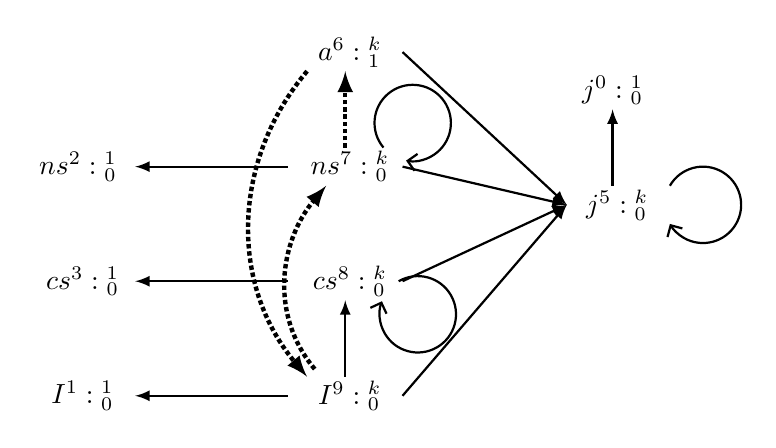
\begin{tikzpicture}[scale=\textwidth/25cm,samples=200]
% Variables Initialization
\draw[] (-7, 1) circle (0pt) node{{ $I^1: {}^1_{0}$}};
\draw[] (-7, 7) circle (0pt) node{{$ns^2: {}^{1}_{0}$}};
\draw[] (-7, 4) circle (0pt) node{{ $cs^3: {}^{1}_{0}$}};
% Variables Inside the Loop
     \draw[] (0, 10) circle (0pt) node{{ $a^6: {}^{k}_{1}$}};
     \draw[] (0, 7) circle (0pt) node{{ $ns^7: {}^{k}_{0}$}};
     \draw[] (0, 4) circle (0pt) node{{ $cs^8: {}^{k}_{0}$}};
     \draw[] (0, 1) circle (0pt) node{{ $I^9: {}^{k}_{0}$}};
     % Counter Variables
     \draw[] (7, 9) circle (0pt) node {{$j^0: {}^{1}_{0}$}};
     \draw[] (7, 6) circle (0pt) node {{ $j^5: {}^{k}_{0}$}};
     %
     % Value Dependency Edges:
     \draw[ thick, -latex,] (0, 1.5)  -- (0, 3.5) ;
     \draw[ ultra thick, -latex, densely dotted,] (0, 7.5)  -- (0, 9.5) ;
     \draw[ thick, -Straight Barb] (1.4, 4) arc (120:-200:1);
     \draw[ thick, -Straight Barb] (8.5, 6.5) arc (150:-150:1);
     \draw[ thick, -Straight Barb] (1, 7.5) arc (220:-100:1);
     \draw[ thick, -latex] (7, 6.5)  -- (7, 8.5) ;
     % Value Dependency Edges on Initial Values:
     \draw[ thick, -latex,] (-1.5, 1)  -- (-5.5, 1) ;
     \draw[ thick, -latex,] (-1.5, 4)  -- (-5.5, 4) ;
     \draw[ thick, -latex,] (-1.5, 7)  -- (-5.5, 7) ;
     %
     \draw[ ultra thick, -latex, densely dotted,] (-1, 9.5)  to  [out=-130,in=130]  (-1, 1.5);
     \draw[ ultra thick, -latex, densely dotted,] (-0.8, 1.7)  to  [out=-230,in=230]  (-0.5, 6.5);
     % Control Dependency
    %  \draw[ thick,-latex] (1.5, 7)  -- (4, 9) ;
    %  \draw[ thick,-latex] (1.5, 4)  -- (4, 9) ;
     \draw[ thick,-latex] (1.5, 7)  -- (5.8, 6) ;
     \draw[ thick,-latex] (1.5, 4)  -- (5.8, 6) ;
     \draw[ thick,-latex] (1.5, 1)  -- (5.8, 6) ;
     \draw[ thick,-latex] (1.5, 10)  -- (5.8, 6) ;
     \end{tikzpicture}
     \caption{}
        \end{centering}
        \end{subfigure}
    \vspace{-0.4cm}
    \caption{(a) The simplified multiple rounds example (b) The program-based dependency graph from $\THESYSTEM$}
    \vspace{-0.5cm}
    \label{fig:multi_graphs}
\end{figure}
%
\end{example}

My static analysis provides an upper bound on the adaptivity for this example as follows.
{\THESYSTEM} constructs a program-based dependency graph, for my example we show this graph in 
Figure~\ref{fig:twoRounds_example}(c).
The edges of this graph are built by considering both control flow and data flow between assigned variables (the algorithm is presented in Section~\ref{subsubsec:static-datadep}). 
The weight of every vertex is estimated by using a reachability-bound estimation algorithm 
(presented in Section~\ref{subsubsec:static-reachability}), which can be symbolic and provide a sound upper bound on the weight of the corresponding vertex in the execution-based dependency graph. 
For instance, the weight $k$ of the vertex $x^{3}$ in Figure~\ref{fig:twoRounds_example}(c) is a sound upper bound on the weight $w_k$ of vertex $x^{3}$ in Figure~\ref{fig:twoRounds_example}(b), with the same starting trace. 
The soundness of this step is proved in Theorem~\ref{thm:addweight_soundness}.

$\THESYSTEM$ search a walk on this graph which over-approximate the adaptivity of the program (this is done by an algorithm
$\pathsearch$ presented in  Section~\ref{subsubsec:static-adapt}). 
%  finds a finite walk on this graph.
% This finite walk traverses the maximum times of query variables, 
% and the visiting time of every vertex on this walk is restricted by its weight.
% The maximum number of vertices visited on this walk which correspond to query variables, is the final estimated adaptivity upper bound, for the program.
For instance, in Figure~\ref{fig:twoRounds_example}(c), $\pathsearch$ first finds a path $l^6:{}^1_1 \to a^5: {}^k_1 \to x^3: {}^k_1$, and then approximate a walk with this path.
Every vertex on this walk is visited once, and the number of vertices with query annotation $1$ traversed in this path is $2$, which is the upper bound we expect.
It is worth to note here that even though the node $x^3$ has weight depending on $k$, 
it is only visited once, similarly for $l^6$, hence the overall upper bound on the adaptivity is 2, as we expect.
%
% \subsection{Implementation}
% \label{subsec:static-implementation}

\cleardoublepage


\section{Further Features}
\label{sec:furthers}
\subsection{Accurate Dynamic Dependency Depth Analysis}
\label{subsec:furthers-dep-depth}
%
The program's adaptivity in our formal model,
% which we define over the program's execution-based dependency graph from the dynamic 
% analysis 
in Definition~\ref{def:trace_adapt} also
 comes across an over-approximation on the program's
 intuitive adaptivity rounds.
It is resulted from difference between its Dependency Depth analysis and the \emph{variable may-dependency} definition.
It occurs when the weight is computed over the traces different from the traces used in 
witness the \emph{variable may-dependency} relation.

As shown in following motivating example, 
\include{examples/multipleRoundsSingle}
% \subsubsection{Examples}
% \label{subsubsec:furthers-dep-depth-examples}
% % \subimport{examples/}{multipleRoundsSingle.tex}
% \include{examples/multipleRoundsSingle}
%%
\subsubsection{Proposed Methodology}
\label{subsubsec:furthers-dep-depth}
% In terms of techniques, our work relies on ideas from both static analysis and dynamic analysis. 
We discuss closely related work in both areas.


1. define the variables dependency relation over two witness traces and an initial trace.
\\
2. Quantify the weight of every edge in the execution-based dependency graph, w.r.t. to the witness traces.
\\

\subsection{Path Sensitive Reachability Bound Analysis}
\label{subsec:furthers-reachability}
In existing static reachability bound analysis, 
it comes across an over-approximation on the estimation due to its path-insensitive nature. 
It occurs when the control flow can be decided in a particular way in front of conditional branches, 
while the static analysis fails to witness. 
As shown in following example, 
\include{examples/multipleRoundsOdd}

% as follo
\subsubsection{Proposed Methodology}
\label{subsubsec:furthers-reachability}
Based on Existing Methodology on reachability bound analysis, design new algorithm computing the 
reachability bounds for every labeled command.
Comparing to just compute the reachability bound for the while loop command, new methodology improves the accuracy of the 
reachability bound for every labeled command.

\subsection{Static Adaptivity Computation towards Completeness}
\label{subsec:furthers-adaptcomplete}
The Algorithm is conditional completeness as proved in appendix, but Algorithm~\ref{alg:adaptscc} isn't.
In the algorithm design at line: in Algorithm~\ref{alg:adaptscc}, an over-approximation happens here. 

As  following motivating example shows.
\subsubsection{Proposed Methodology}
\label{subsubsec:furthers-adaptcomplete-methodology}
%
1. looking into more over-approximated example and summarize the common properties of these examples.
\\
2. Modify the Algorithm~\ref{alg:adaptscc}, targeting the line: 12 of the algorithm. 
The goal is to reduce the over-approximation in computing adaptivity statically.
\subsection{Generalization on Program Resource Cost}
\label{subsec:furthers-cost}

\subsubsection{Introduction and Related Work}
\label{subsubsec:furthers-cost-backgroung}
There are two categories of the program cost analysis, Type-System Based and Static Program Analysis Based. But both of the
works in these two areas fails to recognize the case where program resource consumption is decreased implicitly.
\paragraph*{Type-System Based}
\paragraph*{Static Program Analysis Based}

\subsubsection{Motivating Example}
\label{subsubsec:furthers-cost-example}

\subsubsection{Proposed Methodology}
\label{subsubsec:furthers-cost-methodology}
Following the same system structure as $\THESYSTEM$,
by modifying the restriction on finite walk, compute different resource cost for program.



% 
Based on the language and the trace-based operational semantics in Section~\ref{sec:language},
I present an execution-based program adaptivity analysis in this section.
This analysis formalizes the intuitive \emph{adaptivity} through three steps in 
Section~\ref{subsec:dynamic-methodology}.
% ,~\ref{subsubsec:dynamic-reachability}
% % I  an execution based program analysis in this section.
% and~\ref{subsubsec:dynamic-adapt}.
Then through an example in Section~\ref{subsec:dynamic-examples}, I show that the formalized
% can give the 
adaptivity matches the program's intuitive \emph{adaptivity}.

\subsection{Introduction}
\label{subsec:dynamic-intro}

% In order to formalize a quantitative property w.r.t. the dependency relation in the program, I
% use a three-step analysis methodology developed as follows,
% \\
%  a. The dependency relation between every query, through the methodology of semantic data dependency analysis.
% \\
%  b. The dependency quantity analysis, through the methodology of execution-based data reachability bound analysis. Then 
% \\
%  c. The adaptivity analysis, based on the two analysis results above, 
%  I construct an execution-based dependency graph combining the dependency relation and the dependency quantity
%  and give the formal \emph{adaptivity} definition 
%  for program.
% \\
% The construction of this graph requires me to think about the dependency relation between two queries using what we have at hand - 
% the trace generated in Section~\ref{sec:language}. 
 \paragraph*{Related Work}
 {
My framework constructs an execution-based dependency graph based on the execution traces of a program. I define semantic dependence on this graph by considering (intraprocedural) data and control dependency~\cite{bilardi1996framework,cytron1991efficiently,pollock1989incremental}. 
One related work 
\cite{austin1992dynamic} presents a methodology to construct a dynamic dependency graph (DDG) based on the dynamic execution of a program in an imperative language, where edges represent dependency between instructions. Data dependency, control dependency, storage dependency, and resource dependency between instructions are all considered. My execution-based dependency graph only needs data dependency and control dependency between variable assignment results. 
% Critical path length analysis on DDGs is useful for understanding the scope for parallelization, while we use the length of the longest path to define adaptivity. 
%
DDGs have been used in many other domains. \cite{nagar2018automated} use DDGs to find serializability violations. \cite{hammer2006dynamic} use similar \emph{program dependency graphs} \cite{ferrante1987program} for dynamic program slicing.
\cite{mastroeni2008data} propose ways of constructing different kinds of program slices, by choosing different program dependencies. 
% For example, in either syntactic or semantics sense.
% This abstract dependency is based on properties rather than exact data.
% Aims to give finer and smaller program slice. 
They use a combination of 
static and dynamic dependency graphs but in a manner that is different from how we use the two. Their slicing uses both static and dynamic dependency graphs, while we use the dynamic dependency graph as the basis of a definition, which is then soundly approximated by an analysis based on the static dependency graph.}

{My execution-based data dependency relation definition over variables 
is inspired by the method in \cite{Cousot19a}, where the dependency relation is also identified by looking into the differences on two execution traces. 
However, Cousot excludes timing channels~\cite{SabelfeldM03} and empty observation, which are also not considered as a form of dependency in traditional dependency analysis \cite{DenningD77}.
% In the cases of empty observation and timing channels, the second query is executed 
% in one trace and isn't in another trace by modifying the value of the first query. 
% Then, the second query is indeed dependent on the first query and there exists an
% adaptivity round between the two queries. 
My definition includes timing channels and empty observation by observing both the disappearance and value variation.
}
\paragraph*{Execution-Based Adaptivity Analysis Overview}
To formalize this intuition as a quantitative program property, I develop an execution-based analysis
% I first consider all the possible evaluations of a program --- I do this by 
% I use a trace semantics recording the execution history of programs on some given input --- and I create a dependency graph, where the dependency between different variables (query is also assigned to a variable) is explicit and track which variable is associated with a query request. 
% I then enrich this graph with weights describing the maximal number of times each variable is evaluated in a program evaluation starting with an initial state. The adaptivity is then defined as the length of the walk visiting most query-related variables on this graph. 
% Through two aspects: the execution-based analysis and static-based program analysis.
% In the execution-based analysis, I will formalize the intuitive notion of \emph{adaptivity} as a quantitative 
% property of programs. This analysis is developed 
 in three steps as follows,
 \begin{enumerate}
 \item The first step on \emph{dependency relation} analysis is presented in Section~\ref{subsubsec:dynamic-datadep}.
 In this step, I define the variable \emph{may-dependency} relation based on the trace semantics in Section~\ref{sec:language-os}.
%   to analyze the \emph{dependency relation} between every query, 
%  through the methodology of semantic data dependency analysis.
%  %
%  Specifically through a trace semantics recording the execution history of programs on given input,
%  % --- and I create a dependency graph, 
%  the dependency between different variables (query is also assigned to a variable) is explicitly tracked and 
%  analyzed.
%   and 
%   which variable is associated with a query request. 
% I then enrich this graph with weights describing the maximal number of times each variable is evaluated in a program evaluation starting with an initial state. The adaptivity is then defined as the length of the walk visiting most query-related variables on this graph. 
% In the execution-based analysis, I will formalize the intuitive notion of \emph{adaptivity} as a quantitative 
% property of programs. This analysis is developed 
% \\
 \item In the second step in Section~\ref{subsubsec:dynamic-reachability}, I analyze the \emph{dependency quantity} through the methodology of execution-based reachability bound analysis.
%  As 
% %  analysis, 
% based on the \emph{dependency relation} above.
% This analysis is developed through the methodology of execution-based reachability bound analysis.
% \\
 \item The last step is the intuitive \emph{adaptivity} quantity analysis presented in Section~\ref{subsubsec:dynamic-adapt}.
 According to the two analysis results above, specifically \emph{dependency relation} and \emph{dependency quantity},
 I define the formal \emph{adaptivity} model in definition~\ref{def:trace_adapt} through 
 construct a dependency graph.
%  This analysis is developed through the formal \emph{adaptivity} definition. \\
%  Specifically, I create a dependency graph, where the dependency between different variables (query is also assigned to a variable) is explicit and track which variable is associated with a query request. 
%  I then enrich this graph with weights describing the maximal number of times each variable is evaluated in a program evaluation starting with an initial state. 
%  The adaptivity is then defined as the length of the walk visiting most query-related variables on this graph. 
 \end{enumerate}




\subsection{Methodology}
\label{subsec:dynamic-methodology}

\subsubsection{Data Dependency Analysis}
\label{subsubsec:dynamic-datadep}
\paragraph{Challenge}
\label{para:exe-dep-challenge}
In the data analysis model the programming framework supports, 
%  an \emph{analyst} asks a sequence of queries to the mechanism, and receives the answers to these queries from the mechanism. In this model, the adaptivity I are interested in is the length of the longest sequence of such adaptively chosen queries, among all the queries the data analyst asks. 
  I define that a query is adaptively chosen when it is affected by answers of previous queries. The next thing is to decide how do I define whether one query is "affected" by previous answers, with the limited information I have? As a reminder, 
 when the analyst asks a query, the only known information will be the answers to previous queries and the current execution trace of the program.


There are two possible situations that a query will be "affected",  
either when the query expression directly uses the results of previous queries (data dependency), or when the control flow of the program with respect to a query (whether to ask this query or not) depends on the results of previous queries (control flow dependency).
% As a first step, I give a definition of when one query may depend on a previous query, which is supposed to consider both control dependency and data dependency. We first look at two possible candidates:
% \begin{enumerate}
%     \item One query may depend on a previous query if and only if a change of the answer to the previous query may also change the result of the query.
%     \item One query may depend on a previous query if and only if a change of the answer to the previous query may also change the appearance of the query.
% \end{enumerate}


Since the results of previous queries can be stored or used in variables
which aren't associated to the query request,
it is necessary to track the dependency between queries, through all the program's variables.
In the meantime, the trace-based operational semantics tracks the information,
distinguishing variables which are assigned with query requests.
% and then I can distinguish variables which are assigned with query requests.
In this way, the \emph{may-dependency} relation between queries can be recovered through 
the \emph{may-dependency} relation over all the program's variables.
According to this, I focus on the analysis on the variable \emph{may-dependency} relation in the following of this section.

I give a definition of when one variable \emph{may-depend} on a previous variable with two candidates.
{
\begin{enumerate}
    \item One variable may depend on a previous variable if and only if a change of the value assigned to the previous variable may also change the value assigned to the variable.
    \item One variable may depend on a previous variable if and only if a change of the value assigned to the previous variable may also change the appearance of the assignment command to this variable 
    % in\wq{during?} 
    during execution.
\end{enumerate}
}
%   The first candidate works well by witnessing the result of one query according to the change of the answer of another query. We can easily find that the two queries have nothing to do with each other in a simple example   

{   
% The first situations works well by witnessing the result assigned to variable 
% according to the change of the value assigned to another query. 
% We can easily find that the two queries have nothing to do with each other in a simple example 
% In the first one, by defining the dependency as
The first definition is defined as
% witnessing 
% the query expressions equivalence (or the value equality for non-query assignment )
the witness of a variation on the value assigned to the same variable through two executions,
% assigned to the same variable through two executions, 
according to the change of the value assigned to another variable in pre-trace.
% the situation of data-dependency works well. \wq{long sentence, make it short?}
In particular for query requests, the variation I observe is on the query value instead of on the query requesting results.
% We can find that two queries 
% % have nothing to do with each other in this simple example 
% % depends on each other\wq{not each other, one direction.} 
% satisfy this definition
In 
%this 
the simple program $c_1 =\assign{x}{\query(\chi[2])} ;\assign{y}{\query(\chi[3] + x)}$.
 %
 From our perspective, $\query(\chi[1])$ is different from $\query(\chi[2]))$. Informally, I think $\query(\chi[3] + x)$ may depend on the query $\query(\chi[2]))$, because equipped function of the former $\chi[3] + x$ may depend on the data stored in x assigned with the result of $\query(\chi[2]))$, according to this definition. }
%
% in this example: $c_1 = \assign{x}{\query(0)}; \assign{z}{\query(\chi[x])}$.
% This candidate definition works well 
Nevertheless, the first definition fails to catch control dependency because it just monitors the changes to a query, but misses the appearance of the query when the answers of its previous queries change. 
For instance, it fails to handle $
      c_2 = \assign{x}{\query(\chi[1])} ; \eif( x > 2 , \assign{y}{\query(\chi[2])}, \eskip )
   $, but the second definition can. However, it only considers the control dependency and misses the data dependency. 
  This reminds me to define a \emph{may-dependency} relation between labeled variables by combining the two definitions to capture the two situations.
%
%
% I define the According to the trace-based operational semantics,
%
\paragraph*{Value Difference on Traces}
%
\highlight{
  To define the \emph{may-dependency} relation on two labeled variables, I rely on the limited information at hand - the trace generated by the operational semantics. In this end, 
% So I first define some operations on the trace.
% In order to define the \emph{may-dependency} relation, 
Specifically, we need to be able to observe the difference of the values for each variable
through traces, i.e., through the events contained in traces.
Followed by this, it is necessary to give formal definition on observing this difference through traces.
Given the limitation of previous definition based on limited language,
I present the new definitions on observing the value difference as follows.
These new definitions help in formally capturing the intuitive \emph{adaptivity} precisely, concisely, and efficiently.}
%  in order to observe the evaluation variation in a different way, formally as follows.
\highlight{
\begin{defn}[Value Sequence $\seq(\trace, x^l)$]
  \label{def:vseq}
  \[
\begin{array}{l}
  \seq(\trace :: (x, l, v, \bullet), x^l) \triangleq \seq(\trace)::v  \qquad
  \seq(\trace :: (x, l, v, \qval), x^l) \triangleq \seq(\trace):: \qval \qquad
  \seq([]) \triangleq []\\
  \seq(\trace :: (y, j, \_, \_), x^l) \triangleq \seq(\trace) \quad y \neq x \lor j \neq l 
\end{array}
\]
\end{defn}
%
\begin{defn}[Difference Sequence $\sdiff(\trace_1, \trace_2, x^l )$]
  \label{def:diffseq}
  Let $ s_1 = \seq(\trace_1, x^l) \land s_2 = \seq(\trace_2, x^l)$ be the value sequence of $x^l$ 
  on $\trace_1$ and $\trace_2$, and $s^l$ be the sequence with longer length and $s^t$ the 
  shorter one,
  then their difference sequence is defined as follows,
  \[
    \sdiff(\trace_1, \trace_2, x^l) \triangleq
    \begin{array}{l}
      \{ (s^t[k], s^l[k]) ~|~ 
      % \land 
      % \land 
      s^t[k] \neq s^l[k], k = 0, \ldots, len(s^t)
      \}
      \\
      \cup 
      \{ (\cdot, s^l[k]) ~|~ 
      \len(s^t) \leq \len(s^l)k = len(s^t), \ldots \len(s^l)
      \}
    \end{array}
    \]
\end{defn}
}
\highlight{
  The new analysis compares the difference for all the
  query request evaluation, the non-query assignment evaluation, and the boolean evaluation.
  In this way, all the evaluation information related to the dependency is captured.
  Comparing to the previous works on formalizing adaptivity, which only observe the query difference,
  the new definitions help in analyzing and formalizing the adaptivity more precisely.
}
% A program $c$'s query variables is a subset of 
% its labeled variables, $\qvar(c) \subseteq \lvar(c)$. We have the operator $\tlabel : \mathcal{T} \to \ldom$, which gives the set of labels in every event belonging to the trace.
% Then I introduce a counting operator $\vcounter : \mathcal{T} \to \mathbb{N} \to \mathbb{N}$, 
% % \wq{which counts the occurrence of of a variable in the trace,} 
% which counts the occurrence of a labeled variable in the trace,
% whose behavior is defined as follows,
% \[
% \begin{array}{ll}
% \vcounter(\trace :: (\_, l, \_, \_), l ) \triangleq \vcounter(\trace, l) + 1
% &
% \vcounter(\trace  ::(b, l, v, \bullet), l) \triangleq \vcounter(\trace, l) + 1
% \\
% \vcounter(\trace  :: (x, l, v, \qval), l) \triangleq \vcounter(\trace, l) + 1
% &
% % \vcounter(\trace :: (\_, l', \_, \_), l ) \triangleq \vcounter(\trace, l), l' \neq l 
% % &
% \vcounter(\trace  :: (x, l', v, \bullet), l) \triangleq \vcounter(\trace, l), l' \neq l
% \\
% \vcounter(\trace  :: (b, l', v, \bullet), l) \triangleq \vcounter(\trace, l), l' \neq l
% &
% \vcounter(\trace  :: (x, l', v, \qval), l) \triangleq \vcounter(\trace, l), l' \neq l
% \\
% \vcounter({[]}, l) \triangleq 0
% \end{array}
% \]
  \paragraph{Event Dependency}
\todo{
 To define the \emph{may-dependency} relation on two labeled variables, I rely on the limited information at hand - the trace generated by the operational semantics. In this end, 
 I first define the \emph{may-dependency} between events, and use it as a foundation of the variable may-dependency relation.
\begin{defn}[Events Different up to Value ($\diff$)]
  Two events $\event_1, \event_2 \in \eventset$ are  \emph{Different up to Value}, 
  denoted as $\diff(\event_1, \event_2)$ if and only if:
  \[
    \begin{array}{l}
  \pi_1(\event_1) = \pi_1(\event_2) 
  \land  
  \pi_2(\event_1) = \pi_2(\event_2) \\
  \land  
  \big(
    (\pi_3(\event_1) \neq \pi_3(\event_2)
  \land 
  \pi_{4}(\event_1) = \pi_{4}(\event_2) = \bullet )
  % \qquad \qquad 
  \lor 
  (\pi_4(\event_1) \neq \bullet
  \land 
  \pi_4(\event_2) \neq \bullet
  \land 
  \pi_{4}(\event_1) \neq_q \pi_{4}(\event_2)) 
  \big)
  \end{array}
  \]
  \end{defn}
 %
 We compare two events by defining $\diff(\event_1, \event_2)$. We use $\qexpr_1 =_{q} \qexpr_2$ and $\qexpr_1 \neq_{q} \qexpr_2$ to notate query expression equivalence and in-equivalence, distinct from standard equality. A program $c$'s
%  , its 
 labeled variables 
%  and assigned variables are subsets of 
is a subset of
the labeled variables $\mathcal{LV}$, denoted by $\lvar(c) \in \mathcal{P}(\mathcal{VAR} \times \mathcal{L}) \subseteq \mathcal{LV}$.
% annotated by a label. 
% We use  
%$\mathcal{LVAR} = \mathcal{VAR} \times \mathcal{L} $ 
% $\mathcal{LV}$ represents the universe of all the labeled variables and 
% $\avar(c) \in \mathcal{P}(\mathcal{VAR} \times \mathbb{N}) \subset \mathcal{LV}$ and 
% $\lvar(c) \in \mathcal{P}(\mathcal{VAR} \times \mathcal{L}) \subseteq \mathcal{LV}$ for them. 
We also define the set of query variables for a program $c$, $\qvar: \cdom \to 
\mathcal{P}(\mathcal{LV})$.
\\
A program $c$'s query variables is a subset of 
its labeled variables, $\qvar(c) \subseteq \lvar(c)$. We have the operator $\tlabel : \mathcal{T} \to \ldom$, which gives the set of labels in every event belonging to the trace.
Then I introduce a counting operator $\vcounter : \mathcal{T} \to \mathbb{N} \to \mathbb{N}$, 
% \wq{which counts the occurrence of of a variable in the trace,} 
which counts the occurrence of a labeled variable in the trace,
whose behavior is defined as follows,
\[
\begin{array}{ll}
\vcounter(\trace :: (\_, l, \_, \_), l ) \triangleq \vcounter(\trace, l) + 1
&
\vcounter(\trace  ::(b, l, v, \bullet), l) \triangleq \vcounter(\trace, l) + 1
\\
\vcounter(\trace  :: (x, l, v, \qval), l) \triangleq \vcounter(\trace, l) + 1
&
% \vcounter(\trace :: (\_, l', \_, \_), l ) \triangleq \vcounter(\trace, l), l' \neq l 
% &
\vcounter(\trace  :: (x, l', v, \bullet), l) \triangleq \vcounter(\trace, l), l' \neq l
\\
\vcounter(\trace  :: (b, l', v, \bullet), l) \triangleq \vcounter(\trace, l), l' \neq l
&
\vcounter(\trace  :: (x, l', v, \qval), l) \triangleq \vcounter(\trace, l), l' \neq l
\\
\vcounter({[]}, l) \triangleq 0
\end{array}
\]
% The full definitions of these above operators can be found in the appendix.
\begin{defn}[Event May-Dependency].
\label{def:event_dep}
\\ 
  An event $\event_2$ is in the \emph{event may-dependency} relation with an assignment
  event $\event_1 \in \eventset^{\asn}$ in a program ${c}$
  with a hidden database $D$ and a trace $\trace \in \mathcal{T}$ denoted as 
  %
  $\eventdep(\event_1, \event_2, [\event_1 ] \tracecat \trace \tracecat [\event_2], c, D)$, iff
  %
  \[
    \begin{array}{l}
  \exists \vtrace_0,
  \vtrace_1, \vtrace' \in \mathcal{T},\event_1' \in \eventset^{\asn}, {c}_1, {c}_2  \in \cdom  \sthat
  \diff(\event_1, \event_1') \land 
      \\ \quad
      (
        \exists  \event_2' \in \eventset \sthat 
    \left(
    \begin{array}{ll}   
   & \config{{c}, \vtrace_0} \rightarrow^{*} 
  \config{{c}_1, \vtrace_1 \tracecat [\event_1]}  \rightarrow^{*} 
    \config{{c}_2,  \vtrace_1 \tracecat [\event_1] \tracecat \vtrace \tracecat [\event_2] } 
    % 
   \\ 
   \bigwedge &
    \config{{c}_1, \vtrace_1 \tracecat [\event_1']}  \rightarrow^{*} 
    \config{{c}_2,  \vtrace_1 \tracecat[ \event_1'] \tracecat \vtrace' \tracecat [\event_2'] } 
  \\
  \bigwedge & 
  \diff(\event_2,\event_2' ) \land 
  \vcounter(\vtrace, \pi_2(\event_2))
  = 
  \vcounter(\vtrace', \pi_2(\event_2'))\\
  \end{array}
  \right)
  \\ \quad
  \lor 
  \exists \vtrace_3, \vtrace_3'  \in \mathcal{T}, \event_b \in \eventset^{\test} \sthat 
  \\ \quad
  \left(
  \begin{array}{ll}   
    & \config{{c}, \vtrace_0} \rightarrow^{*} 
      \config{{c}_1, \vtrace_1 \tracecat [\event_1]}  \rightarrow^{*} 
      \config{c_2,  \vtrace_1 \tracecat [\event_1] \tracecat \trace \tracecat [\event_b] \tracecat  \trace_3} 
    \\ 
    \bigwedge &
    \config{{c}_1, \vtrace_1 \tracecat [\event_1']}  \rightarrow^{*} 
    \config{c_2,  \vtrace_1 \tracecat [\event_1'] \tracecat \trace' \tracecat [(\neg \event_b)] \tracecat \trace_3'} 
    \\
    \bigwedge &  \tlabel_{\trace_3} \cap \tlabel_{\trace_3'} = \emptyset
     \land \vcounter(\trace', \pi_2(\event_b)) = \vcounter(\trace, \pi_2(\event_b)) 
    %   \land \event_2 \eventin \trace_3
    % \land \event_2 \not\eventin \trace_3'
    \land \event_2 \in \trace_3
    \land \event_2 \not\in \trace_3'
  \end{array}
  \right)
  )
\end{array}
   \]
% , where ${\tt label}(\event_2) = \pi_2(\event_2)$.
  %  
%
\end{defn}
% \todo{add explnanation}
% \jl{
Our event \emph{may-dependency} relation of 
two events $\event_1 \in \eventset^{\asn}$ and $\event_2 \in \eventset$, 
for a program $c$ and hidden database $D$ is w.r.t to
a trace $[\event_1 ] \tracecat \trace \tracecat [\event_2]$.
The $\event_1 \in \eventset^{\asn}$ is an assignment event because only a change on an assignment event will affect the execution trace, according to our operational semantics.
In order to observe the changes of $\event_2$ under the modification of $\event_1$, this trace 
$[\event_1 ] \tracecat \trace \tracecat [\event_2]$
starts with $\event_1$ and ends with $\event_2$.
% }
{The \emph{may-dependency} relation considers both the value dependency and value control dependency as discussed in 
analysis challenges in Paragraph~\ref{para:exe-dep-challenge}. The relation can be divided into two parts naturally in Definition~\ref{def:event_dep} (line $2-4$, $5-8$ respectively, starting from line $1$). The idea of the event $\event_1$ may depend on $\event_2$ can be briefly described:
I have one execution of the program as reference (See line $2$ and $6$, for the two kinds of dependency). 
When the value assigned to the 
% first variable 
first variable in $\event_1$ is modified, the reference trace $\trace_1 \tracecat [\event_1]$ is modified correspondingly to $\trace_1 \tracecat [\event_1']$.
We use $\diff(\event_1, \event_1')$ at line $1$ to express this modification, which guarantees that $\event_1$ and $\event_1'$ only differ in their assigned values and are equal on variable name and label. We perform a second run of the program by continuing the execution of the same program from the same execution point, 
but with the modified trace $\trace_1 \tracecat [\event_1']$ (See line $3$, $7$). 
The expected may dependency will be caught by observing two different possible changes (See line $4, 8$ respectively) when comparing the second execution with the reference one (similar definitions as in \cite{Cousot19a}). 
\\
% \wq{
% In the first situation, I are witnessing 
In the first part (line $2-4$ of Definition~\ref{def:event_dep}), I witness
% that the value assigned to the second variable in $\event_2$
the appearance of $\event_2'$ in the second execution, and
% a variation in $\event_2$, which changes into $\event_2'$.
a variation between $\event_2$ and $\event_2'$ on their values.
% changes in $\event_2'$.
% \jl{
We have special requirement $\diff(\event_2, \event_2')$, which guarantees that they
have the same variable name and label but only differ 
% % in their assigned value. 
in their evaluated values.
% assigned to the same variable. 
In particularly for queries, if $\event_2$ and $\event_2'$ are 
% query assignment events, then 
generated from query requesting, then $\diff(\event_2, \event_2')$ guarantees that
they differ in their query values rather than the 
% query requesting value. 
query requesting results. 
Additionally, in order to handle multiple occurrences of the same event through iterations of the while loop,
 where  $\event_2$ and $\event_2'$ could be 
in different while loops,
I restrict the same occurrence of $\event_2$'s label in $\trace$ from the first execution with  the occurrence of $\event_2'$'s label in $\trace'$ from the second execution,
through $\vcounter(\vtrace, \pi_2(\event_2))
= 
\vcounter(\vtrace', \pi_2(\event_2'))$ at line $4$.
% }
% }
\\
% \wq{
In the second part (line $5-8$ of Definition~\ref{def:event_dep}), I 
% are witnessing 
witness
the disappearance of $\event_2$ through observing the change of a testing event $\event_b$.
% In order to change the appearance of 
% % and event, the command that generating $\event_2$ must not be executed in 
% 5yhan event, 
To witness
the disappearance, the command that generates $\event_2$ must not be executed in 
the second execution. 
The only way to control whether a command will be executed, is through the change of a guard's 
evaluation result in an if or while command, which generates a testing event $\event_b$ in the first place.
So I observe when
$\event_b$ changes into $\neg \event_b$ in the second execution firstly, 
whether it follows with the disappearance of $\event_2$ in the second trace. We restrict the occurrence of $\event_b$'s label in the two traces being the same
}
% s to the occurrence times of $\event_2'$'s label in the second trace,
through $\vcounter(\trace', \pi_2(\event_b)) = \vcounter(\trace, \pi_2(\event_b))$ to handle the while loop.
% changes in $\event_2'$, have the same variable and label and only differ in their assigned value. 
Again, for queries, I observe the disappearance based on the query value equivalence.
% if $\event_2$ and $\event_2'$ are query assignment events, then 
% they differ in their query value rather than the assigned value. 
% }
%
% \mg{I don't understand this explanation. What are the ``assignment commands associated to the two labelled variables''}
% \jl{revised but need more think}
% Explanation: 
}
\paragraph*{Variable Dependency}
{Considering 
% a program's all possible executions 
all events generated during a program's executions
under an initial trace,
% among all events generated during these executions
% and the variables and labels of these events are 
% corresponding to the two labeled variables,
% evaluations of the assignment commands associated to the two labelled variables respectively, 
as long as there is one pair of events satisfying the \emph{event may-dependency} relation in Definition~\ref{def:event_dep}, 
 I say the two 
related
variables satisfy the \emph{variable may-dependency} relation, in Definition~\ref{def:var_dep}.
}
\begin{defn}[Variable May-Dependency]
    \label{def:var_dep}
\highlight{
    A labeled variable $y^j \in \lvar(c)$ is in the \emph{may-dependency} relation with another
    labeled variable $x^i \in \lvar(c)$ in a program ${c}$, w.r.t. an initial trace $\trace_0 \in \mathcal{T}_0(c)$
    and two witness traces $\trace_1, \trace_2 \in \mathcal{T}$,
    denoted as 
    %
    $\dep(x^i, y^j, \trace_1, \trace_2, \trace_0, {c})$, if an only if
    \[
      \begin{array}{l}
    \exists 
    D \in \dbdom, 
    \trace_0' \in \mathcal{T} \sthat
    (\forall z \neq x \sthat   \env(\trace_0 ) z =   \env(\trace_0') z )
    \\ \quad \land 
     \config{{c}, \vtrace_0} \rightarrow^{*} 
      \config{\clabel{\eskip}^l, \vtrace_0  \tracecat \trace_1 } 
      \land 
      % \config{{c}_1, \vtrace_0' \tracecat [\event_1']}  \rightarrow^{*} 
      % \config{\clabel{\eskip}^l,  
      % \vtrace_0' \tracecat [\event_1] \tracecat \trace_2 }   
      \config{{c}, \vtrace_0'} \rightarrow^{*} 
      % \config{{c}_1, \vtrace_0' \tracecat [\event_1]}  \rightarrow^{*} 
        \config{\clabel{\eskip}^l, \vtrace_0'  \tracecat \trace_2} 
      \land 
        \sdiff(\trace_1, \trace_2, y^j ) \neq \emptyset
      \end{array}
    \]  
  }
    \end{defn}
    Specifically, I define the variables dependency relation over two witness traces and an initial trace. Comparing to 
    the previous \emph{may-dependency} definition, which quantifies overall possible execution traces, the alternative
    definition explicitly relies on two specific witness traces from execution.
    % \\
\highlight{This externalization of the two witness traces also helps in analyzing the dependency quantity through the same 
witness traces as the \emph{may-dependency} relation. 
In this way, the in-accuracy in formalizing the \emph{adaptivity}
is reduced further.}

% \begin{defn}[Variable May-Dependency].
%   \label{def:var_dep}
%   \\
%   A variable ${x}_2^{l_2} \in \lvar(c)$ is in the \emph{variable may-dependency} relation with another
%   variable ${x}_1^{l_1} \in \lvar(c)$ in a program ${c}$, denoted as 
%   %
%   $\vardep({x}_1^{l_1}, {x}_2^{l_2}, {c})$, if and only if.
% \[
%   \begin{array}{l}
% \exists \event_1, \event_2 \in \eventset^{\asn}, \trace \in \mathcal{T} , D \in \dbdom \sthat
% % (\pi_{1}{(\event_1)}, \pi_{2}{(\event_1)}) = ({x}_1, l_1)
% % \land
% % (\pi_{1}{(\event_2)}, \pi_{2}{(\event_2)}) = ({x}_2, l_2)
% \pi_{1}{(\event_1)}^{\pi_{2}{(\event_1)}} = {x}_1^{l_1}
% \land
% \pi_{1}{(\event_2)}^{\pi_{2}{(\event_2)}} = {x}_2^{l_2}% \\ \quad 
% \land 
% \eventdep(\event_1, \event_2, \trace, c, D) 
%   \end{array}
% \]  %
% \end{defn}
\highlight{\paragraph*{Improvements Analysis}
Comparing to previous works,
this new dependency definition is more precise and efficient.
% language and operational semantics design improves the expressiveness, efficiency, and the accuracy to a large extend.
\begin{itemize}
  %   \item \textbf{Improvements on Expressiveness}
  \item \textbf{Improvements on Accuracy}
  \\
  The accuracy is improved in the following senses.
  \\
  By Definition~\ref{def:vseq} and \ref{def:diffseq}, all the information related to the dependency is able to be observed.
  In this sense, the dependency can be analyzing more accurately.
  \\
  By Definition~\ref{def:var_dep}, 
  all the dependency information for variables is captured, including queries. 
  According to this, the adaptivity can be formalized more accurately.
\\
Moreover, the Definition~\ref{def:var_dep} externalized the witness traces. This externalization
helps in analyzing the dependency quantity precisely and improving the adaptivity formalization accordingly.
  %   \\
  % This language is extended over the standard while language. 
  % In this sense, it supports all the general data analysis.
  \item \textbf{Improvements on Efficiency}
  \\
  The efficiency improvements come from the language design, where the program evaluation efficiency is improved. 
  Then efficiency of this execution-based analysis is improved accordingly.
  \end{itemize}
  }
\paragraph*{Dependency Relation through The Two Rounds Example}
\begin{example}[Variable \emph{May-Dependency} Relation in The Two Rounds Data Analysis Example Program]
    In the same $\kw{towRounds(k)}$ example Program,    the analyst asks in total $k+1$ queries to the mechanism in two phases.
    %
    \[         \begin{array}{l}
      \kw{towRounds(k)} \triangleq \\
             \clabel{ \assign{a}{0}}^{0} ;
              \clabel{\assign{j}{k} }^{1} ;\\
              \ewhile ~ \clabel{j > 0}^{2} ~ \edo ~
              \Big(
               \clabel{\assign{x}{\query(\chi[j] \cdot \chi[k])} }^{3}  ;
               \clabel{\assign{j}{j-1}}^{4} ;
              \clabel{\assign{a}{x + a}}^{5}       \Big);\\
              \clabel{\assign{l}{\query(\chi[k]*a)} }^{6}
          \end{array}
          \]    %
    % Queries are of the form $q(e)$ where $e$ is an expression with a special variable $\chi$ representing a possible row. Mainly $e$ represents a function from $X$ to some domain $U$, for example $U$ could be $[-1,1]$ or $[0,1]$. This function characterizes the linear query I are interested in running. As an example, $x \leftarrow q(\chi[2])$ computes an approximation, according to the used mechanism, of the empirical mean of the second attribute, identified by $\chi[2]$. Notice that I don't materialize the mechanism but I assume that it is implicitly run when I execute the query. 
    % \jl{We use $\chi$ to abstract a possible row in the database and }
    % queries are of the form $\query(\qexpr)$, where $\qexpr$ is a special expression 
    In order to analysis the \emph{may-dependency} relation for variable 
    $x^3$ and $a^5$, I first generate the following execution trace with the initial trace
    $\trace_0 = [(k, in, 2, \bullet)]$ as follows,
   %   where $k$ is the 
   %  initial value of input variable $k$ given by user,
   %  we observe the execution trace as
   \\
    $
    \left[\begin{array}{l}
    % \trace_0 \tracecat
     (a, 0, 0, \bullet),
    (j, 1, 2, \bullet),
    (j>0, 2, \etrue, \bullet),
    (x, 3, v_1, \chi[2]*\chi[2]),
    (j, 4, 1, \bullet),
    (a, 5, v_1, \bullet),\\
    (j>0, 2, \etrue, \bullet),
    (x, 3, v_2, \chi[1]*\chi[2]),
    (j, 4, 0, \bullet),
    (a, 5, v_1 + v_2, \bullet),
    (j>0, 4, \efalse, \bullet),\\
    (l, 6, v_3, \chi[2]*( v_1 + v_2))
    \end{array} \right]
    $.
    \\
    We modify the value assigned to $x$ when evaluating the command $ \clabel{\assign{x}{\query(\chi[j] \cdot \chi[k])} }^{3}$
    in the first iteration.
    By manipulating the event in the trace, 
    the event $(x, 3, v_1, \chi[2]*\chi[2])$
    is modified into $(x, 3, v_1', \chi[2]*\chi[2])$ where $v_1 \neq v_1'$.
    Then, through executing the program from the execution point after executing line $3$, we observe another execution trace as follows,
    \\
    $
    \left[\begin{array}{l}
    % \trace_0 \tracecat
     (a, 0, 0, \bullet),
    (j, 1, 2, \bullet),
    (j>0, 2, \etrue, \bullet),
    \highlight{(x, 3, v_1', \chi[2]*\chi[2])},
    (j, 4, 1, \bullet),
    (a, 5, v_1, \bullet),\\
    (j>0, 2, \etrue, \bullet),
    (x, 3, v_2, \chi[1]*\chi[2]),
    (j, 4, 0, \bullet),
    \highlight{(a, 5, v_1' + v_2, \bullet),}
    (j>0, 4, \efalse, \bullet),\\
    (l, 6, v_3, \chi[2]*( v_1' + v_2))
    \end{array} \right]
    $.   
    \\
    In this trace, the event $(a, 5, v_1' + v_2, \bullet),$  is different from $(a, 5, v_1 + v_2, \bullet),$ in the first 
    trace.
    \\
    This change satisfies the Definition~\ref{def:event_dep}, so there exists the variable \emph{may-dependency} relation 
    between variable $x^3$ and $a^5$.
\end{example}
\subsubsection{Data Dependency Quantity Analysis}
\label{subsubsec:dynamic-reachability}
For a program $c$ I compute the reachability bound for every labeled variable overall $c$'s execution traces,
w.r.t. an initial trace as follows,
\[
  rb(x^l) \triangleq \forall \vtrace \in \mathcal{T}_0(c), \trace' \in \mathcal{T} \st \config{{c}, \trace} \to^{*} \config{\eskip, \trace\tracecat\vtrace'} 
  \implies w(\trace) = \vcounter(\vtrace', l) 
  \]
%
$(x^l, w) \in \mathcal{LV} \times (\mathcal{T} \to \mathbb{N})$,
with a labeled variable as first component and
its weight $w$ the second component.
Weight $w$ for
% a labeled variable 
$x^l$ is a function $w : \mathcal{T} \to \mathbb{N}$
mapping from a starting trace to a natural number.
When program executes under this starting trace $\trace$,
$\config{{c}, \trace} \to^{*} \config{\eskip, \trace\tracecat\vtrace'} $, it generates an execution trace $\trace'$.
This natural number is the evaluation times of the labeled command corresponding to the vertex, 
computed by the counter operator $w(\trace) = \vcounter(\vtrace', l)$.


In most data analysis programs $c$ we are interested, there are usually some user input variables, such as $k$ in $\kw{twoRounds}$. 
We denote $\mathcal{T}_0(c)$ as the set of initial traces in which all the input variables in $c$ are initialized, it is also reflected in $\traceW({c})$.    
%
\subsubsection{Adaptivity}
\label{subsubsec:dynamic-adapt}
Given 
a program $c$'s execution-based dependency graph 
% $G_{trace}(c)(\trace) = (\vertxs, \edges, \weights, \qflag)$,
$\traceG({c})$,
we define adaptivity 
with respect to an initial trace $\trace_0 \in \mathcal{T}_0(c)$ by the finite walk in the graph, which has the most query requests along the walk.
We show the definition of a finite walk as follows.
%
% The query length of a walk $k$ is the number of vertices which correspond to query variables in the vertices sequence of this walk. 
% Instead of counting all 
% the vertices in $k$'s vertices sequence, i

\begin{defn}[Finite Walk (k)].
  \label{def:finitewalk}
  \\
%   Given a program $c$'s execution-based dependency graph $\traceG({c})(\trace)$, 
%   a \emph{finite walk} $fw$ in $\traceG({c})(\trace)$ is a sequence of edges $(e_1 \ldots e_{n - 1})$ 
%   for which there is a sequence of vertices $(v_1, \ldots, v_{n})$ such that:
%   \begin{itemize}
%       \item $e_i = (v_{i},v_{i + 1})$ for every $1 \leq i < n$.
%       \item every vertex $v \in \traceV({c}) $ appears in $(v_1, \ldots, v_{n})$ at most 
%       \wq{$\traceW({c})(\trace)$} times.  
%   \end{itemize}
%   %
%   The length of $fw$ is the number of vertices in its vertex sequence, i.e., $\len(k) = n$.
  Given the execution-based dependency graph $\traceG({c}) = (\traceV({c}), \traceE({c}), \traceW({c}), \traceF({c}))$ of a program $c$,
  a \emph{finite walk} $k$ in $\traceG({c})$ is a 
  function $k: \mathcal{T} \to $ sequence of edges.
  For a initial trace $\trace_0 \in \mathcal{T}_0(c)$, 
  $k(\trace_0)$ is a sequence of edges $(e_1 \ldots e_{n - 1})$ 
  for which there is a sequence of vertices 
  $(v_1, \ldots, v_{n})$ such that:
  \begin{itemize}
      \item $e_i = (v_{i},v_{i + 1}) \in \traceE(c)$ for every $1 \leq i < n$.
      \item every $v_i \in \traceV(c)$
      and $(v_i, w_i) \in \traceW(c)$, 
       $v_i$ appears in $(v_1, \ldots, v_{n})$ at most 
    %   \wq{$\traceW({c})(\trace)$} 
    $w(\trace_0)$
      times.  
  \end{itemize}
  %
  The length of $k(\trace_0)$ is the number of vertices in its vertices sequence, i.e., $\len(k)(\trace_0) = n$.
 \end{defn}

We use $\walks(\traceG(c))$ to denote 
% \mg{``the set'', not ``a set''}a set containing all finite walks $k$ in $G$;
the set containing all finite walks $k$ in $\traceG(c)$;
and $k_{v_1 \to v_2} \in \walks(\traceG(c))$ with $v_1, v_2 \in \traceV(c)$ denotes the walk from vertex $v_1$ to $v_2$ . 
\\
We are interested in queries, so we need to recover the 
variables corresponding to queries from the walk. We define the query length of a walk, 
instead of counting all 
the vertices in $k$'s vertices sequence, we just count the number of vertices which correspond to query variables in this sequence.
%
% \mg{I don't understand this definition. Is wrt a single query?if yes, who is chosing the query? Or is it any query?}
% \jl{It is for any query, as long as the vertex is a query variable, in another worlds, this length just counting the number of query variables in the walk, instead of counting all 
% the vertices.}
% \todo{Make the definition clear}
\begin{defn}[Query Length of the Finite Walk($\qlen$)].
\label{def:qlen}
\\
% Given 
% % labelled weighted graph $G = (\vertxs, \edges, \weights, \qflag)$, 
% a program $c$'s execution-based dependency graph $\traceG(c)(\trace)$
%  and a \emph{finite walk} $k$ in $\traceG(c)(\trace)$ with its vertex sequence $(v_1, \ldots, v_{n})$, 
% %  the length of $k$ w.r.t query is defined as:
% The query length of $k$ is the number of vertices which correspond to query variables in $(v_1, \ldots, v_{n})$ as follows, 
% \[
%   \qlen(k) = \len\big( v \mid v \in (v_1, \ldots, v_{n}) \land \qflag(v) = 1 \big)
% \]
% , where $\big(v \mid v \in (v_1, \ldots, v_{n}) \land \qflag(v) = 1 \big)$ is a subsequence of $(v_1, \ldots, v_{n})$.
Given 
% labelled weighted graph $G = (\vertxs, \edges, \weights, \qflag)$, 
the execution-based dependency graph $\traceG({c}) = (\traceV({c}), \traceE({c}), \traceW({c}), \traceF({c}))$ of a program $c$,
 and a \emph{finite walk} 
%  $k$ in $\traceG(c)(\trace)$
 $k \in \walks(\traceG(c))$. 
%  with its vertex sequence $(v_1, \ldots, v_{n})$, 
%  the length of $k$ w.r.t query is defined as:
The query length of $k$ is a function $\qlen(k): \mathcal{T} \to \mathbb{N}$, such that with an initial trace  $\trace_0 \in \mathcal{T}_0(c)$, $\qlen(k)(\trace_0)$ is
the number of vertices which correspond to query variables in the vertices sequence of the walk $k(\trace_0)$
$(v_1, \ldots, v_{n})$ as follows, 
\[
  \qlen(k)(\trace_0) = |\big( v \mid v \in (v_1, \ldots, v_{n}) \land \qflag(v) = 1 \big)|.
\]
% , where $\trace_0 \in \mathcal{T}$ is the initial trace and $\big(v \mid v \in (v_1, \ldots, v_{n}) \land \qflag(v) = 1 \big)$ is a subsequence of $(v_1, \ldots, v_{n})$.
%  $k$'s vertex sequence.
% \mg{If I understand where you want to go, why don't you just use the cardinality of the set above, rather than taking the length of a subsequence?}
% \jl{because the same vertex could have multiple occurrence in the sequence, and we will count all the occurrence instead of just once.
% So the cardinality of set doesn't work.}
\end{defn}
%
%
% \subsection{SSA Transformation and Soundness of Transformation}
% in File {\tt ``ssa\_transform\_sound.tex''}
% \input{ssa_transform_sound}
% %
% %
% The following lemma describes a property of the trace-based dependency graph.
% For any program $c$ with a database $D$ and a initial trace $\trace$,
% the directed edges in its trace-based dependency graph can only be constructed from variable with  
% smaller labels variables of greater ones.
% There doesn't exist backward edges with direction from greater labelled variables to smaller ones.
% \begin{lem}
% \label{lem:edgeforwarding}
% [Edges are Forwarding Only].
% \\
% %
% %
% $$
% \forall \trace \in \mathcal{T}, D \in \dbdom \st G(c, D) =  (\vertxs, \edges, \weights, \qflag) 
% \implies
% \forall (\event', \event) \in \edges \st \event' \eventleq \event
% $$
% %
% \end{lem}
% %
% \begin{proof}
% Proof in File: {\tt ``edge\_forward.tex''}.
% % \input{edge_forward}
% \end{proof}
%
%
% %
% \begin{lem}
% \label{lem:DAG}
% [Trace-based Dependency Graph is Directed Acyclic].
% \\
% %
% $\forall \trace \in \mathcal{T}, D \in \dbdom $, $G(c, D)$ is a directed acyclic graph.
% \end{lem}
%
%
%
\subsection{Adaptivity through An Example}
\label{subsec:dynamic-examples}
\input{examples/twoRounds}
%

% In terms of techniques, our work relies on ideas from both static analysis and dynamic analysis. 
We discuss closely related work in both areas.


%
% \subsection{Implementation}
% \label{subsec:dynamic-implementation}
%
% \cleardoublepage

% In this section, I design a static program analysis framework which soundly approximating the formalized 
\emph{adaptivity} in Section~\ref{sec:dynamic} 
over the same language and the trace-based operational semantics in Section~\ref{sec:language}.
\subsection{Introduction and Related Works}
\label{subsec:static-intro}

\paragraph{{Static analysis for adaptivity}}
% The high level architecture of our static analysis framework is presented in 
%  Figure~\ref{fig:structure}. The input of the analysis is a labeled program P for which the adaptivity A is defined by means of a trace-based definition, as discussed above. In order to estimate an upper bound on A, our program analysis first transforms the program P into static single assignment (SSA) form. The goal of this step is to guarantee that each variable is assigned only once. We show the result of this transformation applied to our two rounds strategy example in Figure~\ref{fig:dcfgraph_tworound}(a). 
%  This transformation, when applied to a loop, introduces some extra variables that serve as intermediate storage. For example, in~\ref{fig:dcfgraph_tworound}(a) there is a new instruction $[(i_3,i_1,i_2),(a_3,a_1,a_2)]$ after the loop. This instruction asserts that the value of the new variables $i_3$ and $a_3$, depending on the execution step, may come from $i_2$ or $i_2$, $a_1$ or $a_2$, respectively. The transformation of a program into SSA form preserves the execution traces, and so, in turns, it preserves the adaptivity. 
% Let us see now how o
Our static analysis provides an upper bound on the adaptivity for this example as follows.
% The high level architecture of our static analysis framework is presented in 
% \jl{Still stick on the two rounds strategy example, which has the aforementioned adaptivity $2$ according our definition, we now present our static analysis which is able to provide an upper bound on the adaptivity, taking the labeled program as input, see Figure~\ref{fig:overview-example}(b). }
% Based on the Ω The input of the analysis is a labeled program P for which the adaptivity $A(c)$ is defined in our formal model as discussed above. 
%  transforms the program P into static single assignment (SSA) form. The goal of this step is to guarantee that each variable is assigned only once. We show the result of this transformation applied to our two rounds strategy example in Figure~\ref{fig:dcfgraph_tworound}(a). 
%  This transformation, when applied to a loop, introduces some extra variables that serve as intermediate storage. For example, in~\ref{fig:dcfgraph_tworound}(a) there is a new instruction $[(i_3,i_1,i_2),(a_3,a_1,a_2)]$ after the loop. This instruction asserts that the value of the new variables $i_3$ and $a_3$, depending on the execution step, may come from $i_2$ or $i_2$, $a_1$ or $a_2$, respectively. The transformation of a program into SSA form preserves the execution traces, and so, in turns, it preserves the adaptivity. 
%  Our framework l ${\THESYSTEM}$
% \jl{Similar as the dependency graph in Figure~\ref{fig:overview-example}(c), {\THESYSTEM} constructs a "may" dependency graph between assigned variables whose dependency both considers control flow and data flow, with the help of some program analysis techniques. To be precise, 
% this algorithm analyzes the data flow relations through variables assigned in every command, based on an abstract control flow graph shown in Figure~\ref{fig:dcfgraph_tworound}(a).} 
% \jl{
 {\THESYSTEM} constructs a program-based dependency graph, for our example we show this graph in Figure~\ref{fig:overview-example}(c). The edges of this graph are built by considering both control flow and data flow between assigned variables (the algorithm is presented in Section~\ref{sec:alg_edgegen}). The weight of every vertex is estimated by using a reachability-bound estimation algorithm (presented in Section~\ref{sec:alg_weightgen}), which can be symbolic and provide a sound upper bound on the weight of the corresponding vertex in the execution-based dependency graph. For instance, the weight $k$ of the vertex $x^{3}$ in Figure~\ref{fig:overview-example}(c) is a sound upper bound on the weight $w_k$ of vertex $x^{3}$ in Figure~\ref{fig:overview-example}(b), with the same starting trace. The soundness of this step is proved in Theorem~\ref{thm:addweight_soundness}.
% Then {\THESYSTEM} computes the adaptivity upper bound through this program-based dependency graph, 
% to approximate the adaptivity defined in the formal model above over the Figure~\ref{fig:overview-example}(b).
% }
%
% through variables assigned in every command, based on an abstract control flow graph shown in Figure~\ref{fig:dcfgraph_tworound}(a).
% \jl{Todo:Add some interesting points of this abstract graph of two round here. Do we want to keep the abstract-cfg here? which is a part of the analysis technique, I think maybe just the final weighted dcfg is enough}
% (1)
%  In this abstract control flow graph, every vertex is a label,
%  corresponding to a label command in the program.
% Each directed 
%  edge represents an abstract transition 
%  between two control locations, i.e., the labels of two commands (we call the labels also control location and they refer to the same thing), 
%  where the second labeled command will be executed after execution of the command with first label.
%  The abstract transition contains a set of difference constraints for variables, generated by abstracting the command of the first labeled.} \wq{The data control dependency graph generated by our algorithm for our two round strategy example is presented in Figure~\ref{fig:dcfgraph_tworound}(b). We can easily see in the graph, that the node $x^{3}$ from the query assignment at line $3$ may depend on the node $j^{1}$ from control flow and node $a^{5}$ may depend on $x^{3}$ from data flow.
%
%  \jl{ Please pay attention to the graph in Figure~\ref{fig:dcfgraph_tworound}(b), every node also has a weight. As a reminder, we also have weight for every node in the dependency graph from our trace semantics in Figure~\ref{fig:overview-example}(c), which stands for the maximal number of times the node (also the statement) appears in the possible traces. In our static analysis, we provide a sound upper bound on this weight from the trace(execution) by performing reachability bound analysis on every statement. The reachability bound is a upper bound on the number of the target command may be reached in a program, which is used as the weight of nodes in our static analysis based data control depdendency graph. The weight can be symbolic, as indicated by the weight $k$ of node $x^{3}$ in Figure~\ref{fig:dcfgraph_tworound}(b).}
 %
% {To be precise, in order to construct the program-based dependency graph,
% $\THESYSTEM$ approximates the vertices and annotations in the first step.
% Then it
% analyzes the data flow relations for approximating the edges between every vertex,
% as well as the quantitative information for approximating the weights of each vertex.}
%  on the dependency depth. Then, it derives a weighted data dependency graph as in Figure~\ref{fig:dcfgraph_tworound}(b), aiming to approximate the graph modeled from execution traces in Figure~\ref{fig:overview-example}(c).
%  Starting from the Figure~\ref{fig:dcfgraph_tworound}(a), $\THESYSTEM$ first generate an abstract control flow graph.
%   In this abstract control flow graph, every vertex is a label,
%  corresponding to a label command in the program.
% Each directed 
%  edge represents an abstract transition 
%  between two control locations, i.e., the labels of two commands (we call the labels also control location and they refer to the same thing), 
%  where the second labeled command will be executed after execution of the command with first label.
%  The abstract transition contains a set of difference constraints for variables, generated by abstracting the command of the first labeled.
%  through this graph and constraint for every transition, 
%
% and compute the transition closure for every abstract transition.
% By solving the closure with the invariants of variables involved in this closure for every transition, 
% we compute the symbolic reachability bound of every commands corresponding to 
% this transition.
 %
 %  (3)
%  in the meantime, this algorithm perform a feasible data-flow analysis through the reachable definition algorithm. 
%  By generating set of all the reachable variables at location of label $l$ in the program $c$.
% For every labelled variable $x^l$ in this set, 
% the value assigned to that variable
% in the assignment command associated to that label is reachable at the entry point of  executing the command of label $l$.
% (4)Then,  by removing the edges between locations where the variables associated to that labeled command isn't reachable from the second location,
% we refined this graph into a weighted-data dependency graph.
 
% $\THESYSTEM$ first performs a simple pass on program collecting the identical vertices
%  and query annotations as in Figure~\ref{fig:overview-example}(c).
% Then, $\THESYSTEM$ performs a feasible data-flow analysis through the reachable definition algorithm, 
% % and refined this graph
% % into the weighted data dependency graph as in Figure~\ref{fig:dcfgraph_tworound}(b), 
% as the approximation of edges in Figure~\ref{fig:overview-example}(b).
%  As a reminder, we also have weight for every node in the dependency graph from our trace semantics as in Figure~\ref{fig:overview-example}(b), which stands for the maximal number of times the node (also the statement) appears over all the possible traces. 
% Similarly,  $\THESYSTEM$ also 
% % infers a symbolic 
% computes a reachability bound as the approximated maximal number of visiting times for each vertex in the program-based dependency graph,
% % by reachability bound for every
% % labeled variable.
% % In our static analysis, we provide a sound upper bound on this weight from the trace(execution) 
% by performing a reachability bound analysis. 
% This reachability bound is a upper bound on the number of the target command may be reached in a program, which is used as the weight of nodes in the program-based dependency graph generated from static analysis.
% % based data control dependency graph. 
% The weight is symbolic, as indicated by the weight $k$ of node $x^{3}$ in Figure~\ref{fig:overview-example}(c).
% Then
% $\THESYSTEM$ generates the program-based dependency graph as in Figure~\ref{fig:overview-example}(c), as a
% % an approximated graph as in 
% approximation for the graph in 
% %  In Figure~\ref{fig:dcfgraph_tworound}(b), every node also has a weight. 
% Figure~\ref{fig:overview-example}(b).}
%  Figure~\ref{fig:dcfgraph_tworound}(b).
%   The upper bound of reaching times of each variable, which performs as the weight of node in the .  estimated by  reachablility it refines this control flow graph into a weighted data-dependency graph, through the data flow and reaching bound analysis results. as well as the reaching times of each variable 
% \wq{The last step of {\THESYSTEM} is that} it finds the longest walk in the weighted data control flow graph w.r.t. the query variables,
% and return the number of query vertices it traversed alongside.
% To be more specific,
% (1)
%  In this abstract control flow graph, every vertex is a label,
%  corresponding to a label command in the program.
% Each directed 
%  edge represents an abstract transition 
%  between two control locations, i.e., the labels of two commands (we call the labels also control location and they refer to the same thing), 
%  where the second labeled command will be executed after execution of the command with first label.
%  The abstract transition contains a set of difference constraints for variables, generated by abstracting the command of the first labeled.
%  (2) Then through this graph and constraint for every transition, we infer the  invariant for every variable,
% and compute the transition closure for every abstract transition.
% By solving the closure with the invariants of variables involved in this closure for every transition, 
% we compute the symbolic reachability bound of every commands corresponding to 
% this transition.
%  (3)
%  in the meantime, this algorithm perform a feasible data-flow analysis through the reachable definition algorithm. 
%  By generating set of all the reachable variables at location of label $l$ in the program $c$.
% For every labelled variable $x^l$ in this set, 
% the value assigned to that variable
% in the assignment command associated to that label is reachable at the entry point of  executing the command of label $l$.
% (4)Then,  by removing the edges between locations where the variables associated to that labeled command isn't reachable from the second location,
% we refined this graph into a weighted-data dependency graph.
%  In the last step, 
 $\THESYSTEM$ search a walk on this graph which overapproximate the adaptivity of the program (this is done by an algorithm
 $\pathsearch$ presented in  Section~\ref{sec:alg_adaptcompute}). 
%  finds a finite walk on this graph.
% This finite walk traverses the maximum times of query variables, 
% and the visiting time of every vertex on this walk is restricted by its weight.
% The maximum number of vertices visited on this walk which correspond to query variables, is the final estimated adaptivity upper bound, for the program.
For instance, in Figure~\ref{fig:overview-example}(c), $\pathsearch$ first finds a path $l^6:{}^1_1 \to a^5: {}^k_1 \to x^3: {}^k_1$, and then approximate a walk with this path.
Every vertex on this walk is visited once, and the number of vertices with query annotation $1$ traversed in this path is $2$, which is the upper bound we expect.
It is worth to note here that even though the node $x^3$ has weight depending on $k$, 
it is only visited once, similarly for $l^6$, hence the overall upper bound on the adaptivity is 2, as we expect.
% By defining it as the finite walk, and restricting the visiting time of each node to its weight, 
% it gives us significant improvement on the accuracy in terms of program cost analysis, comparing with computing the longest weighted path in the state-of-art graph-based program cost analysis works.
%  For analyzing the visiting times of each variable, we 
% \wq{Finally, we reach our analysis algorithm ${\THESYSTEM}$. To bound the longest path is Figure~\ref{fig:simpl-two-round-graph}(c), we decide to build a graph as well. To this end, {\THESYSTEM} constructs a variable-based weighted directed dependency graph where nodes are annotated variables and edges showing the may-dependency of variables. The may-dependency here considers both the data dependency and control dependency and the variables assigned with a query answer has weight $1$ and other variables have no weight. Hence, the estimated upper bound of adaptivity is the weight of most weighted path in the graph.  In Figure~\ref{fig:dcfgraph_tworound}(b), the most weighted path is the dashed one, with weighted node in dashed circle and normal node in standard circle. The weight of that path is $2$. In this example, {\THESYSTEM} produces an upper bound $2$, to the adaptivity $2$ we obtained before, showing its power of a tight estimation. 
% }
%  
% \begin{figure} 
% \centering
%   \begin{subfigure}{.45\textwidth}
%   \begin{centering}
% %   \todo{abstract-cfg for two round}
% \begin{tikzpicture}[scale=\textwidth/18cm,samples=200]
% \draw[] (-5, 10) circle (0pt) node{{ $0$}};
% \draw[] (0, 10) circle (0pt) node{{ $1$}};
% \draw[] (0, 7) circle (0pt) node{\textbf{$2$}};
% \draw[] (0, 4) circle (0pt) node{{ $3$}};
% \draw[] (0, 1) circle (0pt) node{{ $4$}};
% \draw[] (-5, 1) circle (0pt) node{{ $5$}};
% % Counter Variables
% \draw[] (3, 7) circle (0pt) node {\textbf{$6$}};
% \draw[] (3, 4) circle (0pt) node {{ $ex$}};
% %
% % Control Flow Edges:
% \draw[ thick, -latex] (-4.5, 10)  -- node [above] {$a \leq 0$}(-0.5, 10);
% \draw[ thick, -latex] (0, 9.5)  -- node [left] {$j \leq k$} (0, 7.5) ;
% \draw[ thick, -latex] (0, 6.5)  -- node [left] {$\top$}  (0, 4.5);
% \draw[ thick, -latex] (0, 3.5)  -- node [right] {$x \leq \max(\dbdom)$} (0, 1.5) ;
% \draw[ thick, -latex] (0, 1)  -- node [above] {$j \leq j - 1$} (-4.5, 1) ;
% \draw[ thick, -latex] (-5, 1.5)  -- node [left] {$a \leq a + x$} (-0.5, 7)  ;
% \draw[ thick, -latex] (0.5, 7)  -- node [above] {$\top$}  (2.5, 7);
% \draw[ thick, -latex] (3, 6.5)  -- node [left] {$\top$} (3, 4.5) ;
% \end{tikzpicture}
%  \caption{}
%   \end{centering}
%   \end{subfigure}
%   \begin{subfigure}{.5\textwidth}
%   \begin{centering}
%   \begin{tikzpicture}[scale=\textwidth/18cm,samples=200]
% \draw[] (0, 10) circle (0pt) node
% {{ $a^0: {}^1_{0}$}};
% \draw[] (0, 7) circle (0pt) node
% {\textbf{$x^3: {}^{k}_{1}$}};
% \draw[] (0, 4) circle (0pt) node
% {{ $a^5: {}^{k}_{0}$}};
% \draw[] (0, 1) circle (0pt) node
% {{ $l^6: {}^{1}_{1}$}};
% % Counter Variables
% \draw[] (5, 9) circle (0pt) node {\textbf{$j^2: {}^{1}_{0}$}};
% \draw[] (5, 6) circle (0pt) node {{ $j^4: {}^{k}_{0}$}};
% %
% % Value Dependency Edges:
% \draw[ ultra thick, -latex, densely dotted,] (0, 1.5)  -- (0, 3.5) ;
% \draw[ ultra thick, -latex, densely dotted,] (0, 4.5)  -- (0, 6.5) ;
% \draw[ thick, -latex] (0, 7.5)  -- (0, 9.5) ;
% \draw[ thick, -Straight Barb] (1.5, 3.5) arc (120:-200:1);
% \draw[ thick, -Straight Barb] (6.5, 6.5) arc (150:-150:1);
% \draw[ thick, -latex] (5, 6.5)  -- (5, 8.5) ;
% % Control Dependency
% \draw[ thick,-latex] (1.5, 7)  -- (4, 9) ;
% \draw[ thick,-latex] (1.5, 4)  -- (4, 9) ;
% \draw[ thick,-latex] (1.5, 7)  -- (4, 6) ;
% \draw[ thick,-latex] (1.5, 4)  -- (4, 6) ;
% \end{tikzpicture}
% \caption{}
%   \end{centering}
%   \end{subfigure}
%     \vspace{-0.3cm}
%     \caption{(a) Example of data-flow analysis results for two rounds of adaptivity (b) The  weighted data-dependency graph from static analysis result.}
%     \vspace{-0.5cm}
%     \label{fig:dcfgraph_tworound}
% \end{figure}
%
\paragraph*{Related Work} 
Our algorithm in Section~\ref{sec:algorithm} is influenced by many areas of static program analysis such as effect systems, control-flow analysis, and data-flow analysis~\cite{ryder1988incremental}. The idea of statically estimating a sound upper bound for the adaptivity from the semantics is indirectly inspired from prior work on cost analysis via effect systems~\cite{cciccek2017relational,radivcek2017monadic,qu2019relational}. The idea of defining adaptivity using data flow is inspired by the work of graded 
Hoare logic~\cite{gaboardi2021graded}, which reasons about data flows as a resource. 
%
One of the most important ingredients of our work is the estimation of the program-based dependency graph. 
There are many ways to construct a dependency graph statically.
Some of the most related work focuses on the testing of graphical user interfaces (GUIs), using an event graph. For example, \cite{memon2007event} proposes an event-flow model using an algorithm to construct an event-flow graph, representing all the possible event interactions. This event-flow graph has a vertex for every GUI event such as click-to-paste and an edge between pairs of events that can be performed immediately one after the other. Our program-based dependency graph uses the edge to track the may-dependence of one variable with respect to another variable. The main difference is in the way the graph is constructed. {\THESYSTEM} relies on the structure of the target program, while the event-flow model only considers the event type. Another work \cite{arlt2012lightweight} constructs a weighted event-dependency graph, capturing data dependencies between events by analyzing bytecode. Every weighted edge indicates a dependency between two events, meaning one event possibly reads data written by the other event, with the weight showing the intensity of the dependency (the quantity of data involved). Our approach of generating the program-based dependency graph shares the idea of tracking data dependency via static analysis on the source code. However, because of the different domains, we care about assigned variables, and we use the weight in a different way to find a finite walk in the graph.
% WCET on systems: \cite{} 
% [GustafssonEL05]Towards a Flow Analysis for Embedded System C Programs
% --> abstract interpretation.
% --> on embedded system of c program
% [AlbertAGP08] Automatic Inference of Upper Bounds for Recurrence Relations in Cost Analysis
% --> invariant generation through ranking functions
%
% General While langue:
% [BrockschmidtEFFG16]
% Analyzing Runtime and Size Complexity of Integer Programs
% --> invariant generation through ranking functions
% [AliasDFG10] Multi-dimensional Rankings, Program Termination, and Complexity Bounds of Flowchart Programs
% --> invariant generation through ranking functions
% [Flores-MontoyaH14]Resource Analysis of Complex Programs with Cost Equations
% --> invariant generation through cost equations or ranking functions
%
% [GulwaniJK09]Control-flow Refinement and Progress Invariants for Bound Analysis
% --> program abstraction and invariant inference
% []Bound Analysis using Backward Symbolic Execution
% --> program abstraction and invariant inference
%
% [CicekBG0H17]relational Cost Analysis 0
% Monadic refinements for relational cost analysis
% [RajaniG0021]A unifying type-theory for higher-order (amortized) cost analysis
% --> type-system
Moreover, the state-of-art data-flow analysis techniques do not
consider the quantitative information on how many times each variable is dependent on the other. Our weight estimation is inspired by
% (specifically in the case if
% the data-flow is nested in iterations of recursion into consideration). 
 works in program complexity analysis and worst case execution time analysis areas, focusing on analyzing the cost of the entire program. 
The techniques are based on
type system~\cite{CicekBG0H17, RajaniG0021}, Hoare logic~\cite{CarbonneauxHS15}, abstract interpretation~\cite{GustafssonEL05, HumenbergerJK18},
invariant generation through cost equations or ranking functions~\cite{BrockschmidtEFFG16,AlbertAGP08,AliasDFG10,Flores-MontoyaH14}
or a combination of program abstraction and invariant inferring~\cite{GulwaniZ10, SinnZV17,GulwaniJK09}.
In general, these techniques give the approximated upper bound of the program's total running time or resource cost.
However, they failed to consider the case where the cost -- the adaptivity-- could decrease when there isn't a dependency relation between variables.


\subsection{Methodology}
\label{subsec:static-methodology}

% \subsubsection{Abstract Control Flow Graph}
% \label{subsubsec:static-abscfg}

% I discuss the vertices and edge of the
% abstract control flow graph for a program $c$, $\absG(c)$.
% In the abstract control flow graph,
% every 
% vertex corresponds to the unique
% label.
The abstract control flow graph is a control flow graph, with annotations on every edge. It is constructed as follows.
\paragraph*{Vertices of Abstract Control Flow Graph}
The abstract control flow graph enriches the standard control flow graph vertices set with
one extra label, $l_{lex}$ for each program $c$.
Specifically,
the vertices of this graph is the set of $c$'s labels with an exit label $l_{ex}$, 
\[ 
  \absV(c) = labels(c)\cup\{l_{ex}\}
\]
%  corresponding to a label command in the program.

Overall, the vertices can be easily collected and the key point of construction of the abstract execution control flow graph for a program is the abstract execution trace, 
which relies on the abstraction of expression and abstract transition (we also call it abstract event), I will discuss in the following section.

\paragraph*{Edges of Abstract Control Flow Graph}
  The edge in the abstract control flow graph comes from the abstract execution trace of the program. 
  The abstract execution trace, an abstract representation of the execution, consists of a list of abstract transitions. 
  Then, every abstract transition in the abstraction execution trace corresponds to an edge in the abstract control flow graph.
  In another word, the edge $(l_1, dc, l_2)$ in the abstract control flow graph, represents an abstract transition 
 from $l_1$ to $l_2$, with a set of difference constraints $dc$. 
 Also notice, the difference constraints generated during the abstract transition appears in the edge as annotation.
% \wq{
  %  To make it easy to understand, 
  % }  
%
\paragraph{Edge Construction Step 1: Expression Abstraction}

The expression assigned to the variable on the left hand of the assignment command is abstracted to an abstract value: (adopted from the expression abstraction method in paper \cite{sinn2017complexity}). The abstract value is expressed in the form of Difference constraint, denotated as $DC : \mathcal{VAR} \cup \constdom \to \mathcal{\mathcal{VAR} \times (\mathcal{VAR} \cup \constdom) } \times (\mathbb{Z} \cup \{\infty\})$.  $\constdom$ is called the Symbolic Constant defined as $\constdom \triangleq \mathbb{N} \cup \inpvar \cup \{\max{(\dbdom)}\} $, which consists of 
natural numbers $\mathbb{N}$,
the program's input variables $\inpvar$  
and a constant value $\max(\dbdom)$ for estimating the upper bound of variables which are
assigned by queries. 

Give an instance of difference constraint used here,
$DC(\mathcal{VAR}  \cup \constdom) \cup \{\top\}$ represents all the difference constraints over 
variable and symbolic constants. 
% The difference constraint $DC$ over $\mathcal{VAR} \cup \constdom$ 
It is a set of the inequality of form $x \leq y + v$ where $x \in \mathcal{VAR} $, 
$y \in \mathcal{VAR}  \cup \constdom$ and $v \in \mathbb{Z}$. 
This difference constraint is defined in the same way as
\cite{sinn2017complexity}. For concise, I use $\dcdom^{\top}$ to represent the $DC(\mathcal{VAR}  \cup \constdom) \cup \{\top\}$ .


 I show the expression abstraction $\absexpr : \expr \to \mathcal{VAR} \to DC(\mathcal{VAR}  \cup \constdom) \cup \{\top\} $ below.

%  I introduce the following notations and operations first
% % an expression abstraction method based on the expression abstraction in paper \cite{sinn2017complexity}.
% \\
% % is enriched into $\constdom \triangleq \mathbb{N} \cup \inpvar \cup \{\max{(\dbdom)}\} $.
% T
% \\

% represents the set of inequality over all $\mathcal{VAR}  \cup \constdom$. 

% The symbolic constant is enriched into $\constdom \triangleq \mathbb{N} \cup \inpvar \cup \{\max{(\dbdom)}\} $.
% It consists of 
% natural number $\mathbb{N}$,
% the symbolic constants $\inpvar$ (i.e., the set of the program's input variables), 
% and a constant value $\max(\dbdom)$ for estimating the upper bound of variables which are
% assigned by queries.
% \\
% The symbolic constant is enriched into $\constdom \triangleq \mathbb{N} \cup \inpvar \cup \{\max{(\dbdom)}\} $.
% \\

% % $ \absdom: \mathcal{P}(DC(\mathcal{VAR}  \cup \constdom) \cup \{\top \})$:
% \\
% $\constdom: \mathbb{N} \cup \inpvar \cup \{\max{(\dbdom)}\} $ 
% The  constant 
% \\
% % $DC(\mathcal{VAR}  \cup \constdom)$ represents the set of inequality over all $\mathcal{VAR}  \cup \constdom$.
% \\

% \[
%   \begin{array}{ll} 
%     \absexpr(y + c, x)  = x' \leq y + c  & c \in \mathbb{N} \land y \in (VAR \cup \constdom) \\
%     \absexpr(y - c, x)  = x' \leq y - c  & c \in \mathbb{N} \land y \in (VAR \cup \constdom) \\
%     \absexpr(v, x)  = x' \leq v + 0  & v \in (VAR \cup \constdom) \\
%     \absexpr(\aexpr, x) = x' \leq 0 + \infty   & \aexpr \text{ doesn't have any of the forms as above} \\
%     \absexpr(\qexpr, x)  = x' \leq 0 + \max(\dbdom) & \qexpr \text{ is a query expression}  \\
%     \absexpr(\bexpr, x) = x' \leq 0 + 1   & \bexpr \text{ is a boolean expression} \\
%   \end{array}
%   \]
  \[
    \begin{array}{ll} 
      \absexpr(x - v, x)  = x' \leq x - v  & x \in \grdvar \land v \in \mathbb{N} \\
      \absexpr(y + v, x)  = x' \leq y + v  & x \in \grdvar \land v \in \mathbb{Z} \land y \in (\grdvar \cup \constdom) \\
      \absexpr(v, x)  = x' \leq v + 0  & x \in \grdvar \land v \in (\grdvar \cup \constdom) \\
      \absexpr(y + v, x)  = x' \leq y + v & \\
      \grdvar = \grdvar \cup \{y\} & x \in \grdvar \land v \in \mathbb{Z} \land y \notin (\grdvar \cup \constdom)  \\
      \absexpr(\qexpr, x)  = x' \leq 0 + \max(\dbdom) & x \in \grdvar \land \qexpr \text{ is a query expression}  \\
      \absexpr(\bexpr, x) = x' \leq 0 + 1   & x \in \grdvar \land \bexpr \text{ is a boolean expression} \\
      \absexpr(\expr, x) = x' \leq \infty  &  x \in \grdvar \land \expr \text{ doesn't have any of the forms as above} \\
      \absexpr(\expr, x) = \top  &  x \notin \grdvar \\
    \end{array}
    \]
  
  % \wq{ 
    $\grdvar$ is the set of variables used in the guard expression of every while command in the program $c$. 
  % }. 
  In the case 4, if a variable $x$, belonging to the set 
  $\grdvar$ is updated by a variable $y$, which isn't in this set, 
  I add $y$ into the set $\grdvar$ and repeat 
  above procedure  until $\grdvar$ and $\absexpr(\expr, x)$ is stabilized. 
  % \wq{I do not understand this sentence:-(}
  \\
Specifically 
% understanding the intuition, 
we handle a 
% simplified 
normalized guard expression ($ x > 0$ for $x^l \in \lvar_c$)
 in $\ewhile$, and 
%  \wq{I do not understand this sentence:-(}
%  .
% \\
% The counter variables only increase, decrease or reset by expression in the form of arithmetic minus and plus (able to extend to max and min.)
the counter variables only increase, decrease or reset by 
% expression in the form of 
simple arithmetic expression (mainly multiplication, division, minus and plus (able to extend to max and min)). 
This is the same as in paper \cite{sinn2017complexity}. 
\\
For more complex expression assignments, where the counter reset, or calculated from $\elog$, 
multiplication or division, and expressions involving multiple variables, the constraint is approximated as reset of $\infty$.
\\
% This simplification \wq{which part I simplify here?} 
This approximation strategy
doesn't affect our analysis results in our examples. It is easy to extend the normalized expression 
into more complex forms as in \cite{sinn2017complexity}, as well as the 
counter variable manipulation with more advanced expressions.
% \\ 
% The boolean expression in the guard of $\ewhile$ command is normalized into form of $ x > 0$ where $x^l \in \lvar_c$ for some $l$.

\paragraph{Edge Construction Step 2: Abstract Initial and Final State}
%
Abstract initial state: $\absinit(c) \in \ldom$,
Abstract Final State: $\absfinal(c) \in \mathcal{P}(\ldom \times \dcdom^{\top})$

The \emph{Abstract initial state} for a program $c$ is the initial label of this program.
This label corresponds to the first labeled command of this program 
when executing this program.
\\
Given a program $c$, its abstract initial state is computed as follows,
%
\[
  \begin{array}{ll}
    \absinit(\clabel{\assign{x}{\expr}}{}^l)  & = l  \\
    \absinit(\clabel{\assign{x}{\query(\qexpr)}}{}^l)  & = l \\
    \absinit(\clabel{\eskip}^{l})  & = l \\
    \absinit(\eif [b]^l \ethen c_1 \eelse c_2)  & = l \\
    \absinit(\ewhile [b]^l \edo c)  & = l \\
    \absinit(c_1 ; c_2)  & = \absinit(c_1) \\
 \end{array}
 \]
%

The \emph{Abstract Final State} of the program $c$, 
$\absfinal(c) \in \mathcal{P}(\ldom \times \dcdom^{\top})$
is a set of pairs, with a label as first component and a constraint as the second component.
Every pair in $\absfinal(c)$ corresponds to a labeled command of $c$,
and the constraint in this pair is computed by $\absexpr$ in the first step.
\\
Given a program $c$, its final state is computed as follows,
$\absfinal: \cdom \to \mathcal{P}(\ldom \times \dcdom^{\top})$,
% computes the set of Abstract Final State for the command. 
 \[
  \begin{array}{ll}
    \absfinal(\clabel{\assign{x}{\expr}}{}^l)  & = \{(l, \absexpr\eapp (\expr, x))\}  \\
     \absfinal(\clabel{\assign{x}{\query(\qexpr)}}{}^l)  & = \{
      (l, x' \leq 0 + Q_m )\}  \\
     \absfinal(\clabel{\eskip}^{l})  
     & = \{(l, \top)\} \\
     \absfinal(\eif [b]^l \ethen c_1 \eelse c_2)  & = \absfinal(c_1) \cup \absfinal(c_2) \\
     \absfinal(\ewhile [b]^l \edo c)  & = \{(l, \absexpr(\bexpr, \top))\} \\
     \absfinal(c_1 ; c_2)  & =  \absfinal(c_2) \\
 \end{array}
 \]

% \paragraph{Edge Construction Step 3: Program Event Abstraction}
%  I show the abstract event definition, which is generated when computing its abstract execution trace.

% \begin{defn}[Abstract Event]
%   \label{def:abs_event}
%   Abstract Event: 
%   $\absevent \in $
%   $\ldom \times \dcdom^{\top} \times \ldom$
%   is a 
%   % pair of abstract initial state and final state.
%   triple where the first and third components are labels,
%   second component is a constraint from $\dcdom^{\top}$.
%   % the thrid % computed from program's abstract final and initial state, $\absfinal(c)$ and $\absinit(c)$ with formal definition, and algorithm detail in Appendix.
%   %  the constraint and the third corresponds to a final state.
%   \end{defn}
%   Specifically, in an abstract event, 
%   the first label correspond to an initial state, and 
%   the second label and the constraint correspond to an abstract final state.
%  The abstract initial state is a label from $\ldom$.
% The abstract final state is a pair from $\ldom \times \dcdom^{\top}$,  
% where first component is a label from $\ldom$ and the second component is a constraint from $\dcdom^{\top}$.
% %

% %
% Given a program $c$, its abstract initial state,
% and the set of its abstract final state is computed as follows,
% %
% \[
%   \begin{array}{ll}
%     \absinit(\clabel{\assign{x}{\expr}}{}^l)  & = l  \\
%     \absinit(\clabel{\assign{x}{\expr}}{}^l)  & = l \\
%     \absinit(\clabel{\eskip}^{l})  & = l \\
%     \absinit(\eif [b]^l \ethen c_1 \eelse c_2)  & = l \\
%     \absinit(\ewhile [b]^l \edo c)  & = l \\
%     \absinit(c_1 ; c_2)  & = \absinit(c_1) \\
%  \end{array}
%  \]
% %
% Final State Abstraction: 
% $\absfinal: \cdom \to \mathcal{P}(\ldom \times \dcdom^{\top})$,
% computes the set of Abstract Final State for the command. 
%  \[
%   \begin{array}{ll}
%     \absfinal(\clabel{\assign{x}{\expr}}{}^l)  & = \{(l, \absexpr\eapp (\expr, x))\}  \\
%      \absfinal(\clabel{\assign{x}{\query(\qexpr)}}{}^l)  & = \{
%       (l, x' \leq 0 + \max(\dbdom) )\}  \\
%      \absfinal(\clabel{\eskip}^{l})  
%      & = \{(l, \top)\} \\
%      \absfinal(\eif [b]^l \ethen c_1 \eelse c_2)  & = \absfinal(c_1) \cup \absfinal(c_2) \\
%      \absfinal(\ewhile [b]^l \edo c)  & = \{(l, \top)\} \\
%      \absfinal(c_1 ; c_2)  & =  \absfinal(c_2) \\
%  \end{array}
%  \]
%  %
%  \paragraph{Edge Construction Step 3: Abstract Execution Trace Generation}
%  Now, I  extract the abstract execution trace  $\absflow(c)$ for a program, which computes the Abstract Execution Trace for program $c$, as a set of the abstract events $\absevent$.
%  %
%  \begin{defn}[Abstract Execution Trace]
%  \label{def:abs_trace}
%   $\absflow \in \cdom \to \mathcal{P}( \ldom \times DC(\mathcal{VAR}  \cup \constdom) \cup \{\top\}) \times \ldom )$
%   \end{defn}
%  %

 
%    I now show how to compute the abstract execution trace. 
%   For simplicity, I use $\mathcal{P}(\absevent)$ represent the power set of all abstract events, and I have $\absflow(c) \in \mathcal{P}(\absevent)$.
%   I first append a skip command with 
% %  a symbolic label $l_e$, i.e., $\clabel{\eskip}^{l_e}$ at the end of the program $c$, and compute the $\absflow(c) = \absflow'(c')$ for $c'$, where $c' = c;\clabel{\eskip}^{l_e}$ as follows,
% the exist label $l_{ex}$, i.e., $\clabel{\eskip}^{l_{ex}}$ at the end of the program $c$, 
% and compute the $\absflow(c) = \absflow'(c')$ for $c'$, where $c' = c;\clabel{\eskip}^{l_{ex}}$ as follows,
%  %
\paragraph{Abstract Event and Execution Trace} 
 \emph{Abstract Event}: 
   $\absevent \in $
   $\ldom \times \dcdom^{\top} \times \ldom$,
  \emph{Abstract Execution Trace}: $\absflow \in \cdom \to \mathcal{P}( \ldom \times \dcdom^{\top} \times \ldom )$

 The abstract event is generated during computing its abstract execution trace, its type is defined as follows,
 \begin{defn}[Abstract Event]
   \label{def:abs_event}
   Abstract Event: 
   $\absevent \in $
   $\ldom \times \dcdom^{\top} \times \ldom$
   is a 
   % pair of abstract initial state and final state.
   triple where the first and third components are labels,
   second component is a constraint from $\dcdom^{\top}$.
   % the thrid % computed from program's abstract final and initial state, $\absfinal(c)$ and $\absinit(c)$ with formal definition, and algorithm detail in Appendix.
   %  the constraint and the third corresponds to a final state.
   \end{defn}
   Specifically, in an abstract event, 
   the first label correspond to an initial state, and 
   the second label and the constraint correspond to an abstract final state.
  The abstract initial state is a label from $\ldom$.
 The abstract final state is a pair from $\ldom \times \dcdom^{\top}$,  
 where first component is a label from $\ldom$ and the second component is a constraint from $\dcdom^{\top}$.
 %
 For simplicity, we use $\mathcal{P}(\absevent)$ represent the power set of all abstract events, and we have $\absflow(c) \in \mathcal{P}(\absevent)$.

%  Now, we  extract the abstract execution trace  $\absflow(c)$ for a program, which computes the 
 The \emph{Abstract Execution Trace} for program $c$ is a set of the abstract events $\absevent$.
 Its type is formally defined as follows in Definition~\ref{def:abs_trace}.
 %
 \begin{defn}[Abstract Execution Trace]
 \label{def:abs_trace}
  $\absflow \in \cdom \to \mathcal{P}( \ldom \times \dcdom^{\top} \times \ldom )$
  \end{defn}
 %
 The \emph{Abstract Execution Trace} for program $c$ is computed as follows.
 \\
  % We now show how to compute the abstract execution trace. 
 We first append a $\eskip$ command with 
%  a symbolic label $l_e$, i.e., $\clabel{\eskip}^{l_e}$ at the end of the program $c$, and compute the $\absflow(c) = \absflow'(c')$ for $c'$, where $c' = c;\clabel{\eskip}^{l_e}$ as follows,
the label $\lex$, i.e., $\clabel{\eskip}^{l_{ex}}$ at the end of the program $c$, and construct 
the program $c' = c;\clabel{\eskip}^{l_{ex}}$.
Then, we compute the $\absflow(c) = \absflow'(c')$ for $c'$ as follows,
 {\footnotesize
 \[
   \begin{array}{ll}
      \absflow'(\clabel{\assign{x}{\expr}}{}^l)  & = \emptyset  \\
      \absflow'(\clabel{\assign{x}{\query(\qexpr)}}{}^l)  & = \emptyset  \\
      \absflow'([\eskip]^{l})  & = \emptyset \\
      \absflow'(\eif [b]^l \ethen c_t \eelse c_f)  & =  \absflow'(c_t) \cup \absflow'(c_f)
      %   \\ & \quad 
        \cup \{(l, \top,  \absinit(c_t) ) ,  (l, \top, \absinit(c_f)) \} \\
       \absflow'(\ewhile [b]^l \edo c_w)  & =  \absflow'(c_w) \cup \{(l, \top, \absinit(c_w)) \} 
      %  \\ & \quad 
       \cup \{(l', dc, l)| (l', dc) \in \absfinal(c_w) \} \\
       \absflow'(c_1 ; c_2)  & = \absflow'(c_1) \cup  \absflow'(c_2) 
      %  \\ & \quad 
       \cup \{ (l, dc, \absinit(c_2)) | (l, dc) \in \absfinal(c_1) \} \\
   \end{array}
   \]
   }

   Notice $\absflow'([x := \expr]^{l})$, $\absflow'([x := \query(\qexpr)]^{l})$ and $\absflow'([\eskip]^{l})$ are all empty set. 
   For every event $\event$ with label $l$ in an execution trace $\trace$ of program $c$, 
   there is an abstract event in program's abstract execution trace of form $(l, \_, \_)$.  
    I also show the soundness of the abstract execution trace in Appendix.
  %  which says 
  %  \wq{...}
   \begin{lem}[Soundness of the Abstract Execution Trace]
     \label{lem:abscfg_sound}
   Given a program ${c}$, I have:
   %
   \[
     \begin{array}{l}
       \forall \vtrace_0, \trace \in \mathcal{T} ,  \event = (\_, l, \_) \in \eventset \sthat 
   \config{{c}, \trace_0} \to^{*} \config{\eskip, \trace_0 \tracecat \vtrace} 
   \land \event \in \trace 
   \\
   \qquad \implies \exists \absevent = (l, \_, \_) \in (\ldom\times \dcdom^{\top} \times \ldom) \sthat  
   \absevent \in \absflow(c)
   \end{array}
   \]
   \end{lem}
%    This lemma is proved formally in Appendix~\ref{apdx:reachability_soundness}.
% For every event $\event$ with label $l$ in an execution trace $\trace$ of program $c$, 
% there is an abstract event in program's abstract execution trace of form $(l, \_, \_)$. 
This lemma is proved formally in Lemma~\ref{lem:abscfg_sound} in Appendix~\ref{apdx:reachability_soundness}.
\\
For every labeled variable in program $c$, $x^l \in \lvar_c$, there is a unique abstract event in program's abstract execution trace $\absevent \in \absflow(c)$ of form $(l, \_, \_)$. 
\begin{lem}[Uniqueness of the Abstract Execution Trace]
  \label{lem:abscfg_unique}
Given a program ${c}$, I have:
%
\[
  \begin{array}{l}
    \forall \vtrace_0, \trace \in \mathcal{T} ,  \event = (\_, l, \_, \_) \in \eventset^{\asn} \sthat 
\config{{c}, \trace_0} \to^{*} \config{\eskip, \trace_0 \tracecat \vtrace} 
\land \event \in \trace 
\\
\qquad \implies \exists! \absevent = (l, \_, \_) \in (\ldom\times \dcdom^{\top} \times \ldom) \sthat  
\absevent \in \absflow(c)
\end{array}
\]
\end{lem}
This lemma and proof is also 
formalized in Lemma~\ref{lem:absevent_unique} in Appendix~\ref{apdx:reachability_soundness}.

Then, I build the edge for $c$'s abstract control flow graph as follows,
\[
  \absE(c) = \{(l_1, dc, l_2) | (l_1, dc, l_2) \in \absflow(c)\}
  \]

%  I have a pre-processing algorithm to go through the programs and returns the list of labels associating with a loop and whose visiting times need to be analyzed.
%


\paragraph{Abstract Control Flow Graph} 
With the vertices $\absV(c)$ and edges $\absE(c)$ ready, I construct the abstract control flow graph, formally 
% Through a program $c$'s abstract execution trace, its abstract control flow graph is computed 
defined in 
Definition~\ref{def:abs_cfg}.
% Given program $c$ with its abstract control flow $\absflow(c)$, the Abstract Control Flow Graph:
% \\
\begin{defn}[Abstract Control Flow Graph]
\label{def:abs_cfg}
Given a program $c$, 
with its abstract control flow $\absflow(c)$
its abstract control flow graph $\absG(c) =(\absV(c), \absE(c), \absW(c))$ is defined as follows,
\\
% \highlight{
% :
%
% \\
$\absE(c) = \{(l_1, dc, l_2) | (l_1, dc, l_2) \in \absflow(c)\}$,
\\
$\absV(c) = labels(c)\cup\{l_{ex}\}$
\\
 $\absW(c) 
\triangleq \left\{ (l, w) \in \mathbb{L} \times EXPR(\constdom) \right\}$.
% }
% \\
% , where the weight of every label to be computed in the next step.
\end{defn}
% 
% The vertices $\absV(c)$ in this graph are program's labels with an exit label $l_{ex}$.
% Each directed 
%  edge $(l_1, dc, l_2)$ from $l_1$ to $l_2$,
%  represents an abstract transition 
%  between two control locations with a set of difference constraints on it.
% %  , i.e., the labels of two commands (we call the labels also control location and they refer to the same thing), 
% %  where 
% In this transition, the  command labeled with the second location $l_2$, 
%  will be executed after execution of the command with label $l_1$,
% %  The abstract transition contains a set of difference constraints for variables, 
% with the difference constraints generated by abstracting the command of the first label.
% % \\
% % It is easy to show for every $(l_1, dc, l_2) \in \absflow(c)$ such that $l_2 \neq l_e$, $(l_1, l_2) \in flow(c)$. The formal Lemma and proof can be found in Lemma~\ref{lem:flow_to_absflow} in Appendix~\ref{apdx:reachability_soundness}.
Notice I also define the $\absW(c)$ in this graph without giving an actual value.
This $\absW(c)$ is the set of weight for every 
% vertex 
label. The weight is a symbolic expression over the symbolic constant, 
which is the estimated upper bound on the number of visiting time for every control location
through the reachability bound analysis as follows.
%
% It is easy to show for every $(l_1, dc, l_2) \in \absflow(c)$ such that $l_2 \neq l_e$, $(l_1, l_2) \in flow(c)$. The formal Lemma and proof can be found in Lemma~\ref{lem:flow_to_absflow} in Appendix~\ref{apdx:reachability_soundness}.
%
\paragraph*{Abstract Control Flow Graph Through An Example}
%
\begin{example}[The Abstract Control Flow Graph for Two Rounds Data Analysis Program Example]
    For the same two adaptivity rounds example program, 
its generated abstract control flow graph is shown as in Figure~\ref{fig:abscfg_tworound}(b).
For example, the edge $(0, a \leq 0, 1)$ on the top, tells us the command 
$\clabel{\assign{a}{0}}^0$ is executed with next continuation location $1$,
where the 
command $\clabel{\assign{j}{k}}^1$ will be executed next.
The constraint $a \leq 0$ is a difference constraint, generated by abstracting from the assignment command $\assign{a}{0}$,
representing that value of $a$ is less than or equals to $0$ after 
location $0$ before executing command at line $1$. The difference constraint is an inequality relation between, the left-hand side of the inequality talks about the variable before the execution and the right-hand side ascribes those after the execution. 
Look at the $a < a+x $ on the edge $5$ to $2$, which describes the execution of the command at line $5$, which is an assignment $a = a+x$. The $a$ on the left side of $a < a+x$ represents the value of $a$ after the assignment, while the right-hand side $a$ stores the value before the assignment. 
Also, I have while loop, which is a circle $2 \to 4 \to 5 \to 2$ in Figure~\ref{fig:abscfg_tworound}(b). 
Please also look at the edge from $3$ to $4$, which talks about the query! The $x < \max(\dbdom)$ describes the execution of a query request (the command at line 3), the query results stored in $x$ is bounded by $\max(\dbdom)$. 
$\max(\dbdom)$ is the maximal value for query requesting result from the database $DB$. $top$ means there is no assignment executed, for example, I have the difference constraint $\top$ on the edge $2$ to $6$, means at line $2$, there is no assignment (it is a testing guard $j>0$.) 
%
The same way for the rest edges' constructions.
\begin{figure} 
  \centering
  \begin{subfigure}{.7\textwidth}
  \begin{centering}
  {\small
  $
      \begin{array}{l}
            \clabel{ \assign{a}{0}}^{0} ;   
              \clabel{\assign{j}{k} }^{1} ;\\
              \ewhile ~ \clabel{j > 0}^{2} ~ \edo ~ 
              \Big(
               \clabel{\assign{x}{\query(\chi[j])} }^{3}  ;
               \clabel{\assign{j}{j-1}}^{4} ;
              \clabel{\assign{a}{x + a}}^{5}       \Big);\\
              \clabel{\assign{l}{\query(\chi[k]*a)} }^{6}
          \end{array}
  $
  }
  \caption{}
  \end{centering}
  \end{subfigure}
    \begin{subfigure}{.45\textwidth}
    \begin{centering}
  %   \todo{abstract-cfg for two round}
  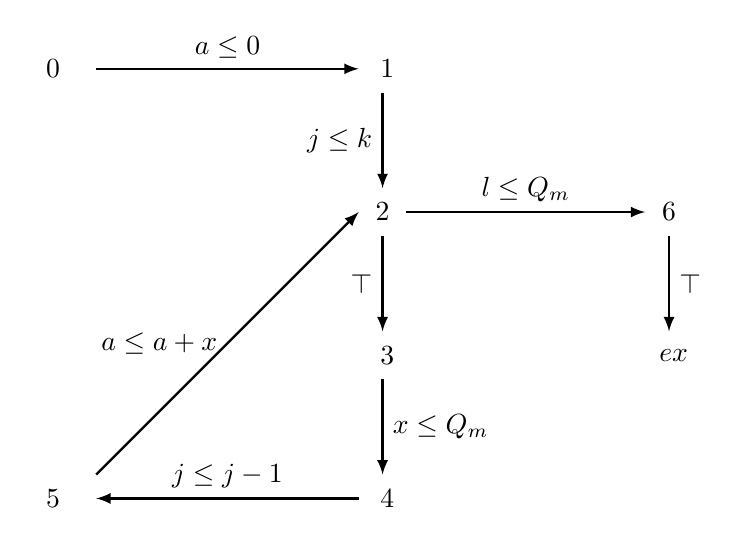
\begin{tikzpicture}[scale=\textwidth/20cm,samples=200]
  \draw[] (-7, 10) circle (0pt) node{{ $0$}};
  \draw[] (0, 10) circle (0pt) node{{ $1$}};
  \draw[] (0, 7) circle (0pt) node{\textbf{$2$}};
  \draw[] (0, 4) circle (0pt) node{{ $3$}};
  \draw[] (0, 1) circle (0pt) node{{ $4$}};
  \draw[] (-7, 1) circle (0pt) node{{ $5$}};
  % Counter Variables
  \draw[] (6, 7) circle (0pt) node {\textbf{$6$}};
  \draw[] (6, 4) circle (0pt) node {{ $ex$}};
  %
  % Control Flow Edges:
  \draw[ thick, -latex] (-6, 10)  -- node [above] {$a \leq 0$}(-0.5, 10);
  \draw[ thick, -latex] (0, 9.5)  -- node [left] {$j \leq k$} (0, 7.5) ;
  \draw[ thick, -latex] (0, 6.5)  -- node [left] {$\top$}  (0, 4.5);
  \draw[ thick, -latex] (0, 3.5)  -- node [right] {$x \leq Q_m$} (0, 1.5) ;
  \draw[ thick, -latex] (-0.5, 1)  -- node [above] {$j \leq j - 1$} (-6, 1) ;
  \draw[ thick, -latex] (-6, 1.5)  -- node [left] {$a \leq a + x$} (-0.5, 7)  ;
  \draw[ thick, -latex] (0.5, 7)  -- node [above] {$l \leq Q_m$}  (5.5, 7);
  \draw[ thick, -latex] (6, 6.5)  -- node [right] {$\top$} (6, 4.5) ;
  \end{tikzpicture}
  \caption{}
    \end{centering}
    \end{subfigure}
    \begin{subfigure}{.45\textwidth}
      \begin{centering}
    %   \todo{abstract-cfg for two round}
    \begin{tikzpicture}[scale=\textwidth/20cm,samples=200]
    \draw[] (-10, 10) circle (0pt) node{{ $0: 1$}};
    \draw[] (0, 10) circle (0pt) node{{ $1: 1$}};
    \draw[] (0, 7) circle (0pt) node{\textbf{$2: k$}};
    \draw[] (0, 4) circle (0pt) node{{ $3: k$}};
    \draw[] (0, 1) circle (0pt) node{{ $4: k$}};
    \draw[] (-10, 1) circle (0pt) node{{ $5: k$}};
    % Counter Variables
    \draw[] (6, 7) circle (0pt) node {\textbf{$6: 1$}};
    \draw[] (6, 4) circle (0pt) node {{ $ex: 1$}};
    %
    % Control Flow Edges:
  \draw[ thick, -latex] (-8, 10)  -- node [above] {$a \leq 0$}(-1.5, 10);
  \draw[ thick, -latex] (0, 9.5)  -- node [left] {$j \leq k$} (0, 7.5) ;
  \draw[ thick, -latex] (0, 6.5)  -- node [left] {$\top$}  (0, 4.5);
  \draw[ thick, -latex] (0, 3.5)  -- node [right] {$x \leq Q_m$} (0, 1.5) ;
  \draw[ thick, -latex] (-1.5, 1)  -- node [above] {$j \leq j - 1$} (-8, 1) ;
  \draw[ thick, -latex] (-8, 1.5)  -- node [left] {$a \leq a + x$} (-1.5, 7)  ;
  \draw[ thick, -latex] (1.5, 7)  -- node [above] {$l \leq Q_m$}  (4.5, 7);
  \draw[ thick, -latex] (6, 6.5)  -- node [right] {$\top$} (6, 4.5) ;
    \end{tikzpicture}
    \caption{}
      \end{centering}
      \end{subfigure}
    \caption{(a) The same $\kw{towRounds(k)}$ program as Figure~\ref{fig:twoRounds_example}
    (b) The abstract control flow graph for $\kw{towRounds(k)}$  (c) The abstract control flow graph with the reachability bound for $\kw{towRounds(k)}$.}
    \vspace{-0.5cm}
    \label{fig:abscfg_tworound}
  \end{figure}
\end{example}

\subsubsection{Static Data Dependency Analysis}
\label{subsubsec:static-datadep}
The new data dependency relation analysis algorithm
is performed on basis of the standard control flow graph.
\highlight{Improved from previous analysis,
this new analysis algorithm combines the reaching definition analysis into the standard data flow analysis.
It designs an improved version of data flow analysis named feasible 
data-flow, estimating a tighter bound on the data dependency relation. 
}
%  of the program, called abstract control flow graph.
In this part, I first show how to generate the standard abstract control flow graph in
Section~\ref{sec:static-cfg}
Then in Section~\ref{sec:static-feasible_flowsto}, 
I present the new feasible 
data-flow analysis
%  reachability-bound analysis algorithm adapted from the newly-designed
% technique in Chapter~\ref{sec:reachability-analysis} 
for estimating the data dependency relation.
Section~\ref{sec:static-dep_compute}
uses the reachability-bound analysis results estimating the dependency quantity
over labeled variables.
%  and
% Section~\ref{sec:static-quantity-edge} uses the same information
% estimating the dependency quantity for the pairs of dependent variables.
In Appendix~\ref{apdx:flowsto_soundness_extend},
this static algorithm is proved as the sound approximation of the variable \emph{may-dependency} relation
in the execution-based analysis in Section~\ref{sec:dynamic-datadep}.
%  before the introduction of  the edge and weight estimation.  

\subsubsection{Standard Control Flow graph}
\label{sec:static-cfg}
% Another operator \mathsf{blocks} 
The standard control flow graph is generated through following steps.
\paragraph*{Vertices Construction}
The vertices of this graph is the set of $c$'s labels , 
\[ 
  \cfgV(c) = labels(c)
\]
%
% Performing a feasible data-flow analysis through the reachable definition algorithm. 
%  By generating set of all the reachable variables at location of label $l$ in the program $c$.
% For every labelled variable $x^l$ in this set, 
% the value assigned to that variable
% in the assignment command associated to that label is reachable at the entry point of  executing the command of label $l$.
\paragraph*{Edges Construction}
The edges set is constructed in following steps.
\\
\textbf{Initial State:}
%
$\cfginit(c) \in \ldom$.
\\
The \emph{initial state} for a program $c$ is the initial label of this program.
This label corresponds to the first labeled command of this program 
when executing this program.
\\
Given a program $c$, its abstract initial state is computed as follows,
%
\[
  \begin{array}{ll}
    \cfginit(\clabel{\assign{x}{\expr}}{}^l)  & = l  \\
    \cfginit(\clabel{\assign{x}{\query(\qexpr)}}{}^l)  & = l \\
    \cfginit(\clabel{\eskip}^{l})  & = l \\
    \cfginit(\eif [b]^l \ethen c_1 \eelse c_2)  & = l \\
    \cfginit(\ewhile [b]^l \edo c)  & = l \\
    \cfginit(c_1 ; c_2)  & = \cfginit(c_1) \\
 \end{array}
 \]
%

\textbf{Final State}: $\cfgfinal(c) \in \mathcal{P}(\ldom)$
The \emph{Final State} of the program $c$, 
$\cfgfinal(c) \in \mathcal{P}(\ldom)$
is a set of labels.
Every label in $\cfgfinal(c)$ corresponds to the exist point of $c$.
\\
Given a program $c$, its final state is computed as follows,
% computes the set of Final State for the command. 
 \[
  \begin{array}{ll}
    \cfgfinal(\clabel{\assign{x}{\expr}}{}^l)  & = \{l\}  \\
     \cfgfinal(\clabel{\assign{x}{\query(\qexpr)}}{}^l)  & = \{l\}  \\
     \cfgfinal(\clabel{\eskip}^{l})  & = \{l\} \\
     \cfgfinal(\eif [b]^l \ethen c_1 \eelse c_2)  & = \cfgfinal(c_1) \cup \cfgfinal(c_2) \\
     \cfgfinal(\ewhile [b]^l \edo c)  & = \{l\} \\
     \cfgfinal(c_1 ; c_2)  & =  \cfgfinal(c_2) 
 \end{array}
 \]

The control flow graph is generated by edges between labels. 
Define $\cfgflow(c): \mathcal{P}(\ldom \times \ldom)$.
%
\[
 \begin{array}{ll}
    \cfgflow(\clabel{\assign{x}{\expr}}{}^l)  & = \emptyset  \\
    \cfgflow(\clabel{\assign{x}{\query(\qexpr)}}{}^l)   & = \emptyset  \\
    \cfgflow(\clabel{\eskip}^{l})  & = \emptyset \\
    \cfgflow(\eif [b]^l \ethen c_1 \eelse c_2) & =  \cfgflow(c_1) \cup \cfgflow(c_2)\cup \{(l, \cfginit(c_1)) , (l, \cfginit(c_2)) \} \\
    \cfgflow(\ewhile [b]^l \edo c)  & =  \cfgflow(c) \cup \{(l, \cfginit(C)) \} \cup \{(l', l)| l' \in \cfgfinal(c) \} \\
    \cfgflow(c_1 ; c_2)  & = \cfgflow(c_1) \cup  \cfgflow(c_2) \cup \{ (l, \cfginit(c_2)) | l \in \cfgfinal(c_1) \} \\
 \end{array}
 \]

The edges for the control flow graph is generated as follows.
Then, I build the edge for $c$'s abstract control flow graph as follows,
\[
  \cfgE(c) = \{(l_1, l_2) | (l_1, l_2) \in \cfgflow(c)\}
  \]

%  I have a pre-processing algorithm to go through the programs and returns the list of labels associating with a loop and whose visiting times need to be analyzed.
%


\paragraph{Control Flow Graph} 
With the vertices $\cfgV(c)$ and edges $\cfgE(c)$ ready, I construct the abstract control flow graph, formally 
% Through a program $c$'s abstract execution trace, its abstract control flow graph is computed 
defined in 
Definition~\ref{def:abs_cfg}.
% Given program $c$ with its abstract control flow $\cfgflow(c)$, the Abstract Control Flow Graph:
% \\
\begin{defn}[Control Flow Graph]
\label{def:cfg_graph}
Given a program $c$, 
with its abstract control flow $\cfgflow(c)$
its abstract control flow graph $\cfgG(c) =(\cfgV(c), \cfgE(c))$ is defined as follows,
\\
% \highlight{
% :
%
% \\
$\cfgE(c) = \{(l_1, dc, l_2) | (l_1, dc, l_2) \in \cfgflow(c)\}$,
\\
$\cfgV(c) = labels(c)$
% }
% \\
% , where the weight of every label to be computed in the next step.
\end{defn}




\subsubsection{Feasible Data-Flow Analysis}
\label{sec:static-feasible_flowsto}
I develop a variant of data flow analysis, called Feasible Data-Flow Generation, which 
considers both the control flow and data flow and
is a sound approximation of the edges in the execution based dependency graph.

% \wq{
\highlight{Improved from previous analysis,
this new analysis algorithm combines the reaching definition analysis on the control flow graph in feasible 
data-flow generation to have a more precise approximation. 
}
% }

% In this step, through 
% % the vertices and edges in 
% $c$'s abstract contrl flow graph $\cfgG(c)$,
%  $\THESYSTEM$ performs a feasible data-flow analysis 
%  using the reachable definition algorithm,
% %  and then Then I generated the set of feasible data-flow between labeled variables based on that.
% and generates the 
% %set of 
% feasible data-flow relation between labeled variables.
% \\
%  By generating set of all the reachable variables at location of label $l$ in the program $c$.
% For every labelled variable $x^l$ in this set, 
% the value assigned to that variable
% in the assignment command associated to that label is reachable at the entry point of  executing the command of label $l$.
% \\
It first defines some operations and then
% In the first step, 
% it 
performs the standard reaching definition analysis given a program $c$, 
on 
% its every label $l$
every label in $\cfgV(c)$.  
% \\
% it performs the standard reaching definition analysis given a program $c$, on its every label $l$.
% \\
% Another operator \mathsf{blocks} 
%
% Performing a feasible data-flow analysis through the reachable definition algorithm. 
%  By generating set of all the reachable variables at location of label $l$ in the program $c$.
% For every labelled variable $x^l$ in this set, 
% the value assigned to that variable
% in the assignment command associated to that label is reachable at the entry point of  executing the command of label $l$.
% \paragraph{Generate CFG}
%  \begin{def}
%   \label{def:init_label}
%   Define $\mathsf{init}$: Command -> label, which returns the initial label of the statement. 
% \[
%  \begin{array}{ll}
%     init([x := e]^{l})  & = l  \\
%      init([x := q(e)]^{l})  & = l \\
%      init([skip]^{l})  & = l \\
%      init([if [b]^l then C_1 else C_2]^{l})  & = l \\
%      init([while [b]^l do C]^{l})  & = l \\
%      init(C_1 ; C_2)  & = init(C_1) \\
%  \end{array}
%  \]
% \end{def}
%   Define $\mathsf{final}$: Command -> Powerset(label), which returns the final labels of the statement. 
%  \[
%  \begin{array}{ll}
%     final([x := e]^{l})  & = \{l\}  \\
%      final([x := q(e)]^{l})  & = \{l\}  \\
%      final([skip]^{l})  & = \{l\} \\
%      final([if [b]^l then C_1 else C_2]^{l})  & = final(C_1) \cup final(C_2) \\
%      final([while [b]^l do C]^{l})  & = \{l\} \footnote{while terminates after b evaluates to false} \\
%      final(C_1 ; C_2)  & =  final(C_2) \\
%  \end{array}
%  \]
% \paragraph*{Blocks and Defs}
%  Define block B to be either the command of the form of assignment, skip, or test of the form of $[b]^{l}$.\\
%  Define $\mathsf{blocks}$ : command -> Powerset(Block)
%  \[
%  \begin{array}{ll}
%     blocks([x := e]^{l})  & = \{[x := e]^{l}\}  \\
%      block([x := q(e)]^{l})  & = \{[x := q(e)]^{l}\}  \\
%      blocks([skip]^{l})  & = \{[skip]^{l}\} \\
%      blocks([if [b]^l then C_1 else C_2]^{l})  & = {[b]^{l}} \cup blocks(C_1) \cup blocks(C_2) \\
%      blocks([while [b]^l do C]^{l})  & = \{[b]^{l}\} \cup blocks(C) \\
%      blocks(C_1 ; C_2)  & = blocks(C_1) \cup  blocks(C_2) \\
%  \end{array}
%  \]
%  Define $\mathsf{labels}$ to get the labels of blocks.
%  \[
%    labels(C) = \{l | [B]^{l} \in blocks(C) \}
%  \]  

% The control flow graph is generated by edges between labels. Define $\mathsf{flow}$: command -> P (label $\times$ label ).

% \[
%  \begin{array}{ll}
%     flow([x := e]^{l})  & = \emptyset  \\
%      flow([x := q(e)]^{l})  & = \emptyset  \\
%      flow([skip]^{l})  & = \emptyset \\
%      flow([if [b]^l then C_1 else C_2)  & =  flow(C_1) \cup flow(C_2)\cup \{(l, init(C_1)) , (l, init(C_2)) \} \\
%      flow([while [b]^l do C)  & =  flow(C) \cup \{(l, init(C)) \} \cup \{(l', l)| l' \in final(C) \} \\
%      flow(C_1 ; C_2)  & = flow(C_1) \cup  flow(C_2) \cup \{ (l,init(C_2)) | l \in final(C_1) \} \\
%  \end{array}
%  \]
 
%  Define block B to be either the command of the form of assignment, skip, or test of the form of $[b]^{l}$.\\
%  Define $\mathsf{blocks}$ : command -> Powerset(Block)
\paragraph*{Blocks and Defs}
The block, 
is either the command of the form of assignment, skip, or a test of the form of $[b]^{l}$, 
% and $block$ of program $c$ is 
denoted by $\mathsf{blocks}(c)$
the set of all the blocks 
in program $c$, where  $\mathsf{blocks}: \cdom \to \mathcal{P}(\cdom \cup \clabel{\bexpr}^{l})$.
Then it generates the set of feasible data-flow between labeled variables with detail in Definition~\ref{def:feasible_flowsto}, 
based on $\live(l, c)$ for every label in a program $c$ and its blocks $\mathsf{blocks}$.
\\
The details are as follows.

The operator $\mathsf{blk} : \cdom \to \mathsf{blocks}$ gives all the blocks in program $c$.
\\
 \[
 \begin{array}{ll}
  \mathsf{blk}(\clabel{\assign{x}{\expr}}{}^l)  & = \{(\clabel{\assign{x}{\expr}}{}^l)\}  \\
  \mathsf{blk}(\clabel{\assign{x}{\query(\qexpr)}}{}^l)  & = \{(\clabel{\assign{x}{\query(\qexpr)}}{}^l)\}  \\
  \mathsf{blk}([\eskip]^{l})  & = \{[\eskip]^{l}\} \\
  \mathsf{blk}(\eif [b]^l \ethen c_1 \eelse c_2)  & = {[b]^{l}} \cup \mathsf{blk}(c_1) \cup \mathsf{blk}(c_2) \\
  \mathsf{blk}(\ewhile [b]^l \edo c)  & = \{[b]^{l}\} \cup \mathsf{blk}(c) \\
  \mathsf{blk}(C_1 ; C_2)  & = \mathsf{blk}(c_1) \cup  \mathsf{blk}(c_2) \\
 \end{array}
 \]
%  $label^{?}$ is label $\cup \{?\}$.\\
%  Define $\mathsf{kill}$: $blocks \to \mathcal{P}(\mathcal{VAR} \times LABEL \cup \{?\})$, which produces the set of labelled variables of assignment destroyed by the block.
\paragraph*{Kills and Gens}
The operator $\mathsf{kill}$: $\mathsf{blocks} \to \mathcal{P}(\mathcal{VAR} \times \ldom \cup \{?\})$ produces the set of labelled variables of assignment destroyed by the block.
 \\
  % Define $\mathsf{gen}$: $blocks \to \mathcal{P}(\mathcal{VAR} \times LABEL \cup \{?\})$, which generates the set of labelled variables generated by the block.
  The operator $\mathsf{gen}$: $\mathsf{blocks} \to \mathcal{P}(\mathcal{VAR} \times \ldom \cup \{?\})$ generates the set of labelled variables generated by the block.
  \\
  % Define $defs(x)(c): \mathcal{VAR} \to LABEL$, gives all the labels where assigns value to variable x in the target program $c$. 
  % The operator  $defs(c): \mathcal{VAR} \to \ldom$ gives all the labels where assigns value to variable in $c$. 
 \[
 \begin{array}{ll}
  \mathsf{kill}(\clabel{\assign{x}{\expr}}{}^l)  & = \{ (x, ?) \} \cup \{ (x, l') | l' \in defs(x) \} \\
  \mathsf{kill}(\clabel{\assign{x}{\query(\qexpr)}}{}^l)  & = \{ (x, ?) \} \cup \{ (x, l') | l' \in defs(x) \}  \\
  \mathsf{kill}([\eskip]^{l})  & = \emptyset \\
  \mathsf{kill}([ [b]^l ]^{l})  & =  \emptyset
 \end{array}
 ~~
  \begin{array}{ll}
    \mathsf{gen}(\clabel{\assign{x}{\expr}}{}^l)  & = \{ (x, l) \}  \\
    \mathsf{gen}(\clabel{\assign{x}{\query(\qexpr)}}{}^l)  & = \{ (x, l) \}  \\
    \mathsf{gen}([\eskip]^{l})  & = \emptyset \\
    \mathsf{gen}([ [b]^l ]^{l})  & =  \emptyset 
 \end{array}
 \]
 The $?$ is a placeholder for the unknown label need to be comptued.
%  Define $in(l)$, $out(l)$: LABEL$ \to \mathcal{VAR} \times LABEL \cup \{?\}$ for every block in program $c$ is computed as follows,
%  \[
%  \begin{array}{lll}
%     in(l)  & = \{ (x, ?) | x^l \in \lvar_c \land  l = \cfginit(c) \}  
%     \cup \{ out(l')|  | (l',\_, l) \in \cfgE \land  l \neq \cfginit(c)\}  \\
%      out(l)  & =  gen(B^{l}) \cup \{ in(l) \setminus kill(B^l)  \} & B^l \in blocks(c)   
%  \end{array}
%  \]
%  computing $in(l)$ and $out(l)$ for every $B^l \in blocks(c) $, and repeating these two step
% until the $in(l)$ and $out(l)$ are stabilized for every $B^l \in blocks(c) $
%  I use $\live_{in}(l,c)$ and $\live_{out}(l, c)$ denote the stabilized results for the command of label $l$ in program $c$. 
%  Define $defs(x)(c): \mathcal{VAR} \to LABEL$, gives all the labels where assigns value to variable x in the target program $c$.
% Define $defs(x)(c): \mathcal{VAR} \to \ldom$, gives all the labels where assigns value to variable x in the target program $c$.
% \\
%  Define $in(l)$, $out(l)$: $ \ldom \to \mathcal{VAR} \times LABEL \cup \{?\}$ for every block in program $c$ is computed as follows,
\paragraph*{In and Out}
The operator  $in(l)$, $out(l)$: $ \ldom \to \mathcal{LV} \cup \{?\}$ for every block in program $c$ is defined as follows,
 \[
 \begin{array}{ll}
    % in(l)  & = \{ (x, ?) | x^l \in \lvar_c \land  l = \cfginit(c) \}  
    in(l)  & = \{ x^{?} | x^l \in \lvar_c \land  l = \cfginit(c) \}  
    \cup \{ out(l')|  | (l',\_, l) \in \cfgE(c) \land  l \neq \cfginit(c)\}  \\
     out(l)  & =  \mathsf{gen}(B^{l}) \cup \{ in(l) \setminus \mathsf{kill}(B^l)  \}  
 \end{array}
 \]
computing $in(l)$ and $out(l)$ for every $B^l \in \mathsf{blk}(c) $, and repeating these two steps
until the $in(l)$ and $out(l)$ are stabilized for every $B^l \in \mathsf{blk}(c) $
%  I use $\live_{in}(l,c)$ and $\live_{out}(l, c)$ denote the stabilized results for the command of label $l$ in program $c$. 
 I use $\live(l,c)$ to represent 
% $\live_{in}(l,c)$ in the other part of the paper.
denote the stabilized result of $in(l)$ at label $l$ in program $c$. 
% The $\live_{in}(l,c)$ and $\live_{out}(l, c)$ is computed by the Standard worklist algorithm. (For simplicity, I use $\live(l,c)$ to represent $\live_{in}(l,c)$ in the other part of the paper.}
\\
% The $\live_{in}(l,c)$ and $\live_{out}(l, c)$ 
\paragraph{Reaching definition computation}
This step generates set of all the reachable variables at location of label $l$ in the program $c$.
The $\live(l, c)$ represent the analysis result, which is the set of 
reachable labeled variables in program $c$ at the location of label $l$.
For every labelled variable $x^l$ in this set, 
the value assigned to that variable
in the assignment command associated to that label is reachable at the entry point of  executing the command of label $l$.

The stabilized $in(l)$ and $out(l)$ for program $c$, as well as $\live(l, c)$,
is computed by the standard worklist algorithm with detail as below. 
% For simplicity, I use $\live(l,c)$ to represent $\live_{in}(l,c)$ in the other part of the paper.
\begin{enumerate}
    \item Initializing in[l]=out[l]=$\emptyset$
    \item Initializing in[entry label] = $\emptyset$
    \item Initializing a work queue, contains all the blocks in $c$
    \item while |W| != 0 \\
         pop l in W\\
          old = out[l]\\
          in(l) =  out(l') where $(l',\_, l) \in \cfgE(c)$\\
           out(l) = $\mathsf{gen}$($b^l$) $\cup$ (in(l) - $\mathsf{kill}$($b^l$) ) where $b^l$ in $\mathsf{blk}(c)$   \\
          if (old != out(l)) W= W $\cup$ \{l'| (l,l') in $(l',\_, l) \in \cfgE(c)$\}\\
          end while
\end{enumerate}
%
% computing $in(l)$ and $out(l)$ for every $B^l \in blocks(c) $, and repeating these two step
% until the $in(l)$ and $out(l)$ are stabilized for every $B^l \in blocks(c) $
%  I use $\live_{in}(l,c)$ and $\live_{out}(l, c)$ denote the stabilized results for the command of label $l$ in program $c$. 
% The $\live_{in}(l,c)$ and $\live_{out}(l, c)$ is computed by the Standard worklist algorithm. (For simplicity, I use $\live(l,c)$ to represent $\live_{in}(l,c)$ in the other part of the paper.
%%
\paragraph{Feasible Data-Flow Generation}
by using the results of Reaching definition analysis results, specifically $\live(l, c)$ for every label in a program $c$, I refine the vertices and edges in the $\cfgG$ graph 
by generating the set of feasible data-flow between labeled variables as follows,
%
%   \[
%  \begin{array}{ll}
%     dcdg([x := e]^{l})  & = \{ (y^i, x^l) | y \in VAR(e) \land (y,i) \in \live_{in}(l) \}  \\
%      dcdg([x := q(e)]^{l})  & = \{ (y^i, x^l) | y \in VAR(e) \land (y,i) \in \live_{in}(l) \}  \\
%      dcdg([skip]^{l})  & = \emptyset \\
%      dcdg([if [b]^l then C_1 else C_2)  & =  dcdg(c_1) \cup dcdg(c_2)\\ & \cup \{(x^i,y^j) | x \in VAR(b) \land (x,i) \in \live_{in}(l) \land ([y = \_]^j) \in blocks(c_1) \} \\
%      &\cup \{(x^i,y^j) | x \in VAR(b) \land (x,i) \in \live_{in}(l) \land ([y = \_]^j) \in blocks(c_2) \} \\
%      dcdg([while [b]^l do c)  & =  dcdg(c) \cup \{(x^i,y^j) | x \in VAR(b) \land (x,i) \in \live_{in}(l) \land ([y = \_]^j) \in blocks(C) \} \\
%      dcdg(c_1 ;c_2)  & = dcdg(c_1) \cup  dcdg(c_2) \\
%  \end{array}
%  \]
%
\begin{defn}[Feasible Data-Flow]
  \label{def:feasible_flowsto}
  Given a program $c$ and two labeled variables $x^i, y^j$  in this program, 
  $\flowsto(x^i, y^j, c)$ is 
    {\footnotesize
    \[
   \begin{array}{ll}
    \flowsto(x^i, y^j, \clabel{\assign{x}{\expr}}{}^l)  & \triangleq (x^i, y^j) \in \{ (y^i, x^l) | y \in \mathsf{FV}(\expr) 
    % \land (y,i) \in \live(l, \clabel{\assign{x}{\expr}}^l) \}  \\
    \land y^i \in \live(l, \clabel{\assign{x}{\expr}}^l) \}  \\
    \flowsto(x^i, y^j, \clabel{\assign{x}{\query(\qexpr)}}{}^l)  & \triangleq (x^i, y^j) \in \{ (y^i, x^l) | y \in \mathsf{FV}(\qexpr) 
    % \land (y,i) \in \live(l,\clabel{\assign{x}{\query(\qexpr)}}^l) \}  \\
    \land y^i \in \live(l,\clabel{\assign{x}{\query(\qexpr)}}^l) \}  \\
    \flowsto(x^i, y^j, [\eskip]^{l})  & = \emptyset \\
    \flowsto(x^i, y^j, \eif ([b]^l, c_1, c_2))  & \triangleq \flowsto(x^i, y^j, c_1) \lor \flowsto(x^i, y^j, c_2) \\ 
        & \lor (x^i, y^j) \in
       \{(x^i,y^j) | x \in \mathsf{FV}(b) \land 
      %  (x,i) 
      x^i \in \live(l, \eif ([b]^l, c_1, c_2)) \land  y^j \in \lvar(c_1) \\
    %   ([y = \_]^j) \in \mathsf{blk}(c_1) \} \\
       &\lor (x^i, y^j) \in \{(x^i,y^j) | x \in \mathsf{FV}(b) \land 
      %  (x,i) 
      x^i\in \live(l, \eif ([b]^l, c_1, c_2))  \land  y^j \in \lvar(c_2) \\
    %   \land ([y = \_]^j) \in \mathsf{blk}(c_2) \} \\
       \flowsto(x^i, y^j, \ewhile [b]^l \edo c_w)  & \triangleq  \flowsto(x^i, y^j, c_w)  \lor
       \\ & 
       (x^i, y^j) \in  \{(x^i,y^j) | x \in \mathsf{FV}(b) \land 
      %  (x,i) 
      x^i \in \live(l,   \ewhile [b]^l \edo c_w) \land  y^j \in \lvar(c_w) \\
    %   ([y = \_]^j) \in \mathsf{blk}(c_w) \} \\
       \flowsto(x^i, y^j, c_1 ;c_2)  & \triangleq \flowsto(x^i, y^j, c_1) \lor \flowsto(x^i, y^j, c_2) \\
   \end{array}
   \]
   }
   \end{defn}
%
This \emph{Feasible Data-Flow} relation is a sound approximation 
of the variable \emph{May-Dependency} relation over labeled variables for every program.
The soundness is proved
in Appendix~\ref{apdx:flowsto_soundness}.
%
\subsubsection{Data Dependency Relation Estimation}
\label{sec:static-dep_compute}
%
For any program $c$ and two labeled variables $x^i, y^j$  in this program, 
$x^i, y^j$  is in the estimated dependency relation if and only if they satisfy
$\flowsto(x^i, y^j, c)$.

As introduce in the third step in Section~\ref{sec:static-overview},
this set is used in Section~\ref{sec:static-adapt} to estimate
the execution-based dependency graph.
As introduced in third step of this analysis framework in Section~\ref{sec:static-overview},
this information will be used in constructing the program-based dependency graph, to estimate the execution-based dependency graph for the program.
For easy understanding,
I reveal the estimated directed edges construction below
% vertex and weight construction of this estimated graph below
and presents the formal definition later. 
% for each vertex in $\progV(c)$,
This estimated directed edges set is defined as a set of triples 
% $\progW(c) \in \mathcal{P}(\mathcal{LV} \times \mathcal{LV} \times EXPR(\constdom))$ 
$\progE(c) \in \mathcal{P}(\mathcal{LV} \times \mathcal{A}_{\lin} \times \mathcal{LV})$,
Each directed edge is defined between vertices $({x}_1^{i}, w_1)$  
and $({x}_2^{j}, w_2)$ 
where ${x}_1^{i}, {x}_2^{j} \in \lvar(c)$, and they are in the estimated dependency relation
% is the set of pairs 
% The weight for each vertex in $\progV(c)$ is computed 
% indicating a directed edge from the first vertex to the second one in each pair
as follows,
\highlight{
  \[
    \progE^0(c) \triangleq 
    \left\{ 
    ({x}_1^{i}, w, {x}_2^{j}) \in \mathcal{LV} \times 
    \mathcal{A}_{\kw{in}} \times \mathcal{LV}
    ~ \middle\vert ~
    \begin{array}{l}
      {x}_1^{i}, {x}_2^{j} \in \lvar(c)
    \land
      % \\
      \exists n \in \mathbb{N}, z_1^{r_1}, \cdots, z_n^{r_n} \in \lvar_{{c}} \sthat
      n \geq 0 \land
      \\
      \flowsto(x^i,  z_1^{r_1}, c) 
      \land \cdots \land \flowsto(z_n^{r_n}, y^j, c) 
    \end{array}
    \right\}
    \]
}
The weight $w$ for every edge in this definition is a placeholder.
It will be computed in Section~\ref{sec:static-quantity}.
We prove that this estimated directed edge set $\progE(c)$ is a sound approximation of the 
edge set in $c$'s Execution-Based Dependency Graph 
in Appendix~\ref{apdx:adapt_soundness}.

% \paragraph*{Edges Estimation}
% Then I define the estimated directed edges
% % for each vertex in $\progV(c)$,
% between vertices in $\progV(c)$,
% as a set of pairs 
% % $\progW(c) \in \mathcal{P}(\mathcal{LV} \times \mathcal{LV} \times EXPR(\constdom))$ 
% $\progE(c) \in \mathcal{P}(\in \mathcal{LV} \times \mathcal{LV})$
% % is the set of pairs 
% % The weight for each vertex in $\progV(c)$ is computed 
% indicating a directed edge from the first vertex to the second one in each pair
% as follows,
% \highlight{
%   \[
%     \progE(c) \triangleq 
%     \left\{ 
%     ({x}_1^{i}, {x}_2^{j}) \in \mathcal{LV} \times \mathcal{LV}
%     ~ \middle\vert ~
%     \begin{array}{l}
%       {x}_1^{i}, {x}_2^{j} \in \progV(c)
%     \land
%       % \\
%       \exists n \in \mathbb{N}, z_1^{r_1}, \cdots, z_n^{r_n} \in \lvar_{{c}} \sthat  
%       n \geq 0 \land
%       \\
%       \flowsto(x^i,  z_1^{r_1}, c) 
%       \land \cdots \land \flowsto(z_n^{r_n}, y^j, c) 
%     \end{array}
%     \right\}
%     \]
% }
% This estimated directed edge set $\progE(c)$ is a sound approximation of the 
% edge set in $c$'s execution-based dependency graph, which is proved 
% in Appendix~\ref{apdx:adapt_soundness}.
%  \begin{defn}[Feasible Data-Flow]
%   \label{def:feasible_flowsto}
%     {\footnotesize
%     \[
%    \begin{array}{ll}
%       dcdg(\clabel{\assign{x}{\expr}}{}^l)  & = \{ (y^i, x^l) | y \in FV(e) \land (y,i) \in \live_{in}(l, \clabel{\assign{x}{\expr}}^l) \}  \\
%        dcdg(\clabel{\assign{x}{\query(\qexpr)}}{}^l)  & = \{ (y^i, x^l) | y \in FV(e) \land (y,i) \in \live_{in}(l,\clabel{\assign{x}{\query(\qexpr)}}^l) \}  \\
%        dcdg([\eskip]^{l})  & = \emptyset \\
%        dcdg([\eif [b]^l \ethen c_1 \eelse c_2)  & =  dcdg(c_1) \cup dcdg(c_2)\\ & \cup 
%        \{(x^i,y^j) | x \in FV(b) \land (x,i) \in \live_{in}(l) \land ([y = \_]^j) \in blocks(c_1) \} \\
%        &\cup \{(x^i,y^j) | x \in FV(b) \land (x,i) \in \live_{in}(l) \land ([y = \_]^j) \in blocks(c_2) \} \\
%        dcdg([\ewhile [b]^l \edo c)  & =  dcdg(c) \cup \{(x^i,y^j) | x \in FV(b) \land (x,i) \in \live_{in}(l) \land ([y = \_]^j) \in blocks(C) \} \\
%        dcdg(c_1 ;c_2)  & = dcdg(c_1) \cup  dcdg(c_2) \\
%    \end{array}
%    \]
%    }
%    \end{defn}
%    For any two labeled variables $x^i, y^j$ in a program $c$, 
%   %  it is easy to see that there is a one-on-one correspondence between 
%   %  $\flowsto$ relation of the two variables, and the $dcdg$ analysis result on $c$.
%   I use $\flowsto()$ denote if they have a feasible data-flow relation in Definition~\ref{def:flowsto}.
%    \begin{defn}[Feasible Data-Flow ($\flowsto$)]
%    \label{def:flowsto}
%    \[
%    \forall c \in \cdom, x^i, y^j \in \lvar_c \sthat  
%    \flowsto(x^i, y^j, c) \iff (x^i, y^j) \in dcdg(c)
%    \]
%    \end{defn}
  %  This soundness is proved in Proof~\ref{pf:rd_soundness} in Appendix~\ref{apdx:rd_soundness}.
  %  For any two labeled variables in a program $c$, it is easy to see that there is a one-on-one correspondence between 
  %  $\flowsto$ relation of the two variables, and the $dcdg$ analysis result on $c$.
  %  \begin{thm}[Soundness of the Feasible Data-Flow Analysis]
  %  \label{thm:rd_soundness}
  %  \[
  %  \forall c \in \cdom, x^i, y^j \in \lvar_c \sthat  
  %  \flowsto(x^i, y^j, c) \iff (x^i, y^j) \in dcdg(c)
  %  \]
  %  \end{thm}
  %  This soundness is proved in Proof~\ref{pf:rd_soundness} in Appendix~\ref{apdx:rd_soundness}.
  \paragraph*{Example}
% Still looking at the Figure~\ref{fig:adapfun_tworound}(c), 
% and taking the edge $(l^6, a^5)$ for example.
% By $\flowsto(l^6, a^5, c)$, I can see $a$ is used directly in the query expression $\chi[k]*a$,
% in the assignment command $\clabel{\assign{l}{\query(\chi[k]*a)}}^l$,
% i.e., $a \in FV(\chi[k]*a)$.
% Also, from the Reaching definition analysis, I know $a^5 \in \live(6, two-round)$.
% Then I have $\flowsto(l^6, a^5, c)$ and construct the edge $(l^6, a^5)$.
% And same way for constructing the rest edges.
%
The edge $(l^6, a^5)$ in Figure~\ref{fig:twoRounds_example}(c) is constructed by this definition.
% and take  for example.
By $\flowsto(l^6, a^5, c)$, I can see $a$ is used directly in the query expression $\chi[k]*a$,
in the assignment command $\clabel{\assign{l}{\query(\chi[k]*a)}}^l$,
i.e., $a \in FV(\chi[k]*a)$.
Also, from the reaching definition analysis, I know $a^5 \in \live(6, \kw{twoRounds(k)})$.
Then I have $\flowsto(l^6, a^5, c)$ and construct the edge $(l^6, a^5)$.
And the same way for constructing the rest edges. Also, the edge $(x^3,j^5)$ in the same graph represents the control flow, 
caught by the $\flowsto$ relation.
% Still looking at the Figure~3(c) in main paper, 
% and taking the edge $(l^6, a^5)$ for example.
% By $\flowsto(l^6, a^5, c)$, I can see $a$ is used directly in the query expression $\chi[k]*a$,
% in the assignment command $\clabel{\assign{l}{\query(\chi[k]*a)}}^l$,
% i.e., $a \in FV(\chi[k]*a)$.
% Also, from the Reaching definition analysis, I know $a^5 \in \live(6, two-round)$.
% Then I have $\flowsto(l^6, a^5, c)$ and construct the edge $(l^6, a^5)$.
% And same way for constructing the rest edges. Also, the edge $(x^3,j^5)$ in the same graph represents the control flow, caught by our $\flowsto$ relation.
%
  \subsubsection{Improvements Analysis}
  \label{sec:static-dep-improvements}
  \highlight{
    This new data dependency estimation algorithm is more precise and efficient than previous static analysis.
% language and operational semantics design improves the expressiveness, efficiency, and the accuracy to a large extend.
% \todo{Add details}
\begin{itemize}
  %   \item \textbf{Improvements on Expressiveness}
  %   \\
  % This language is extended over the standard while language. 
  % In this sense, it supports all the general data analysis.
  \item \textbf{Improvements on Efficiency}
  \\
  New analysis architecture does not rewrite the program into SSA version.
\\
  New analysis technique does not pre-collect the variables generated during the program.
\\
  New analysis technique does unfold the while loop and perform analysis for each iteration of the loop, 
  instead, it only performs the analysis on the while body once.
  \\
In the three senses above, the efficiency is improved significantly.
  \item \textbf{Improvements on Accuracy}
  Comparing to previous dependency estimation method,
  new analysis technique uses the reachable definition algorithm.
  This algorithm improves the accuracy 
  on the approximating the data dependency relation.
  Let us see a simple example, a program $ [x = 0]^{1}; [x=2]^{2};  [y = x+1]^{3}$. 
The standard data flow analysis 
tells us that both the labeled variable $x^{1}$ and $x${2} may flow to $y^{3}$, which will result in an unnecessary edge ($x^{1}, y^{3}$). The result of reaching definition 
can help us eliminate this kind of edge by telling us, at line $3$, only variable $x^{2}$ is reachable. 
  \end{itemize}
  }

\subsubsection{Static Reachability Bound Analysis}
\label{subsubsec:static-reachability}

In order to estimate weight for every vertex in the program-based dependency graph,
we perform the symbolic reachability bound analysis on the abstract control flow graph and add weight as shown in Figure~\ref{fig:abscfg_tworound}(c). 
% This because
% the vertices in the two graph share the same unique label, the line number.
% We would like to generate the closure of every edge, which is an equality relation between variables.  Solving this closure gives us the reachability bound for this edge. With all the bound for all the edges in the abstract control flow graph, we can calculate the weight for every vertex in this graph. For example, we show the closure generated for the edge $(4, j < j - 1, 5)$, 
% $\absclr(4, 5) = \varinvar(j)$. The invariant for variable $j$, $\varinvar(j)$ used here is 
% $\varinvar(j) = k * \absclr(1, 2)$, which is generated by all the difference constraints involving $j$ in the graph. Notice the $k$ in $\varinvar(j)$ comes from considering both difference constraint $j<=k$ from edge (1,2) and $j<=j-1$ from (4,5), which intuitively reflects the while loop whose counter is set to $k$ at the beginning and decreases by 1 at each iteration.
% We first generate the invariant for every variable showing up in the difference constraint and not user defined. For example, in the Figure~\ref{def:abscfg_tworound}(b), there are three variables $a$, $x$, $j$ that we will generate invariant for. We show the invariant for the counter $k$, which is $j = k$. 
% $\absclr(1, 2) = 1$
% \\
% => 
% $\absclr(4, 5) = k$
% using the difference constraint on the edges for all 
% through the edges in $\absG(c)$, which correspond to $c$'s abstract transition between labels.
% We infer the invariant for every variable, and compute the transition closure for every abstract transition. By solving the closure
% with the invariants of variables involved in this closure for every transition, we compute
% the symbolic reachability bound of every commands corresponding to this transition. Specifically, this analysis can be performed in four steps:
%  Variable Modification Tracking, Local Bounds Computation,
% Invariant Inference and Closure Generation, and Reachability Bound Computation,
% 
% We present the details of invariant, closure generation, and reachability bound computation as follows.
% with details as follows.
% \\
% %
% 1.  Variable Modification Tracking: collecting the dc for where each variable is increased, decreased and reset: 
% \\
% 2. Local Bounds Computation: 
% \\
% 3. Invariant Inference and Closure Generation
% \\
% 4. Reachability Bound Computation,
% %
% \paragraph*{Variable Modification Tracking}
% Identify the abstract events where each variable is increased, decreased and reset:
% \\
% $\inc: \mathcal{VAR} \to \mathcal{P}(\absevent) $
% the set of the abstract events where the variable increase.
% \\
% $\inc(x) = \{(\absevent, c) | \absevent = (l, l', x' \leq x + v)\}$
% \\
% $\reset: \mathcal{VAR} \to \mathcal{P}(\absevent) $
% The set of the abstract events where the variable is reset.
% \\
% $\dec: \mathcal{VAR} \to \mathcal{P}(\absevent) $
% The set of abstract events where the variable decrease.
% % \\
% % $\dec(x) = \{(\absevent, c) | \absevent = (l, l', x' \leq x - v)\}$
% \\
% $Incr(v) \triangleq \sum\limits_{(\absevent, c) \in \inc(v)}\{\absclr(\absevent) \times v\}$
% %
% \paragraph*{Local Bounds}
% Given a program $c$ with its abstract control flow graph 
% $\absG(c) = (\absV, \absE)$
% \\
% Local Bounds Computation:
% $\locbound: \absevent \to \mathcal{VAR} \cup \constdom$.
% %
% \[ 
% \begin{array}{ll}
%   \locbound(\absevent) \triangleq 1 
%   & \absevent \notin SCC(\absG(c))
%   \\
%   \locbound(\absevent) \triangleq (x, v) 
%   & \absevent \in SCC(\absG(c)) \land \absevent \in \dec(x) \land  \absevent = (\_, \_ , x' \leq x - v) \\
%   \locbound(\absevent) \triangleq (x, \max(\dec(x))) 
%   & \absevent \in SCC(\absG(c)) \land 
%   \absevent  \notin \bigcup_{x \in \mathcal{VAR}} \dec(x)
%   \land \absevent \notin SCC(\absG(c) \setminus \dec(x)) 
% \end{array}
%   \]
%   The first case is straightforward. Since variable's visiting time outside of any while loop is at most 1, we do not need to analyze the visiting times of every node in the graph from phase 1.
%   The second and third step is guaranteed by the \emph{Discussion on Soundness} in Section 4 of \cite{sinn2017complexity}.
%   Then soundness proof is in Lemma~\ref{lem:local_bound_sound} in appendix~\ref{apdx:reachability_soundness}.
% %
% \paragraph*{Invariant Inference and Closure Generation }
% Then, computing the bound invariants for variables and the transition closures for abstract events:
% \\ 
% $ \varinvar: \mathcal{VAR} \cup \constdom \to EXPR(\constdom)$
% \\
% $\absclr: \absevent \to EXPR(\constdom)$
% \\
% Then, the symbolic invariant for each variable 
% as well as the symbolic transition closure for each transition is calculated as follows:
% \[ 
% \begin{array}{lll}
%   \varinvar(x) & \triangleq c & c \in \constdom \\
%   \varinvar(x) & \triangleq Incr(v) + \max(\{\varinvar(a) + c | (t, a, c) \in \reset(x)\}) & c \notin \constdom
% \end{array}
% \]
% %
% \begin{defn}
%   \label{def:transition_closure_base}
% \[ 
% \begin{array}{lll}
%   \absclr(\absevent) 
%   & \triangleq x / v & \\ 
%   & \locbound(\absevent) = (x, v) \in \constdom \times \mathbb{N} & \\
%   \absclr(\absevent) 
%   & \triangleq (Incr(x) + 
%   \sum\limits_{(\absevent', y, v') \in \reset(x)}
%   \absclr(\absevent') \times \max(\varinvar(y) + v', 0) ) / v & \\
%   & \locbound(\absevent) = (x, v) \land x \notin \constdom & 
% \end{array}
%   \]
% \end{defn}
% %
% \paragraph*{Improved Variable Modification Tracking}
% Instead of just identifying the abstract events where each variable is reset,
% this improvement identifies the chain of the events where a given variable is reset by the 
% variables of the abstract events through the chain.
% \\
% $\resetchain: \mathcal{VAR} \to \mathcal{P}(\mathcal{P}(\absevent)) $
% The set of the chain of abstract events where the variable is reset through the chain.
% % \\
% % $Incr(v) \triangleq \sum\limits_{(\absevent, c) \in \inc(v)}\{\absclr(\absevent) \times v\}$
% %
% \paragraph*{Improved Invariant Inference and Closure Generation}
% Then, computing the bound invariants for variables and the transition closures for abstract events:
% \\ 
% $ \varinvar: \mathcal{VAR} \cup \constdom \to EXPR(\constdom)$
% \\
% $\absclr: \absevent \to EXPR(\constdom)$
% \\
% Then, the symbolic invariant for each variable 
% as well as the symbolic transition closure for each transition is calculated as follows:
% \[ 
% \begin{array}{lll}
%   \varinvar(x) & \triangleq c & c \in \constdom \\
%   \varinvar(x) & \triangleq Incr(v) + \max(\{\varinvar(a) + c | (t, a, c) \in \reset(x)\}) & c \notin \constdom
% \end{array}
% \]
% %
% \begin{defn}
%   \label{def:transition_closure}
% \[ 
% \begin{array}{lll}
%   \absclr(\absevent) 
%   & \triangleq x / v & \\ 
%   & \locbound(\absevent) = (x, v) \in \constdom \times \mathbb{N} & \\
%   \absclr(\absevent) 
%   & \triangleq \Big(
%     \sum\limits_{y \in \{ y ~|~ 
%     ch \in \resetchain(x), (l_1, x, y, v, l_2) \in ch \} } Incr(x) & \\
%     & \quad + 
%   \sum\limits_{ch \in \resetchain(x)}
%   \big( \min\limits_{\absevent' \in ch}({\absclr(\absevent')}) \times 
%   \max(\varinvar(y) + \sum\limits_{(l_1, x, y, v, l_2) \in ch } v, 0)\big) \Big) / v & \\
%   & \locbound(\absevent) = (x, v) \land x \notin \constdom & 
% \end{array}
%   \]
% \end{defn}
  %
% \paragraph*{Adding the Reachability Bounds for Every Vertex in the Data-Control Flow Graph}
% Updating the weight of every vertex in the $\progG(c) = (\progV, \progE, \progW, \progF)$ for program $c$ generated from phase 1. 
% For every $x^l \in \progV$, find the abstract event $\absevent \in \absflow(c)$ of the form $(l, \_, \_)$, updating the $\progW(x^l) $ by the transition closure of this event.
% \\
% \paragraph*{Reachability Bound Computation}
% With all the closures for all the edges of the abstract control flow graph, we can solve them to obtains the reachability bound of every edges. We decide the weight for every vertex in the abstract control flow graph by using the bound of the edges which head out from this vertex, by taking the max of the bound from these involving edges. For instance,   
% By the constraint on the edge $(4, j \leq j - 1, 5)$, we get bound $k$ for this edge.
% Then, we assign vertex $4$ by reachability bound $k$, as in Figure~\ref{fig:abscfg_tworound}(c). 
% Another interesting vertex is $2$, which has more than one edge heading out from it, $(2, \top, 3)$ and $(2,\top, 6)$. For the weight for vertex $2$, we choose the max between the bound $k$ from $(2,\top, 3)$ and $1$ from $(2,\top, 6)$.
% we first infer its local bound as variable $j$.
% Then by solving the invariant for variable $j$,
% we infer the value bound for $j$, which is $k$.
% Then the reachability bound for this abstract transition, (i.e., edge $4, j \leq j - 1, 5$) 
% is computed as $k$ as well through Definition~\ref{def:abs_trace}.
% \\
% $
% \progW(x^l) 
%   \triangleq \absclr(\absevent)
% $
% Through the transition closure computed above, 
% The weight of every label in 
% % Then we update 
% the program $c$'s abstract control flow graph,
% $\absG(c) =(\absV, \absE, \absW)$
% is 
% computed as the maximum over all the abstract events $\absevent \in \absE$ heading out from this vertex, formally as follows.
% % by annotating each vertex with a symbolic weight. 
% % This weight corresponds to 
% %reachability bounds of
% \\
% $\absW 
% \triangleq \left\{ (l, w) \in \mathbb{N} \times EXPR(\constdom) | w = \max\limits_{\absevent = (l, \_, \_)} \{ \absclr(\absevent)\} \right\}$.
% % \\
% \paragraph*{Example}
% Still looking at the two-round example as in Figure~\ref{fig:abscfg_tworound}(b) where 
% each label $l$ is added with a weight by $absW$.
% This weight represents the  maximum reaching times of this location $l$, in the other word,
% the estimated maximum visiting times of the command labeled with $l$.
% For example, looking at the vertex $1$,
% by analysis steps, since it isn't in any SCC, it's estimated reachability bound is computed as $1$.
% However, for the vertex $4$ which is involved in an SCC, the reachability bound is inferred in another way.
% By the constraint on the edge $4, j \leq j - 1, 5$,
% we first infer its local bound as variable $j$.
% Then by solving the invariant for variable $j$,
% we infer the value bound for $j$, which is $k$.
% Then the reachability bound for this abstract transition, (i.e., edge $4, j \leq j - 1, 5$) 
% is computed as $k$ as well through Definition~\ref{def:abs_trace}.
% In this abstract control flow graph, every vertex is a label,
% corresponding to a label command in the program.
% Each directed 
% edge represents an abstract transition 
% between two control locations, 
% i.e., the labels of two commands (we call the labels also control location and they refer to the same thing), 
% where the second labeled command will be executed after execution of the command with first label.
% For example, the edge $0, a \leq 0, 1$ on the top, represents,
% from location $0$, the command 
% $\clabel{\assign{a}{0}}^0$ is executed with next continuation location $1$,
% where the 
% command $\clabel{\assign{j}{k}}^1$ will be executed next.
% The constraint $a \leq 0$ is generated by abstracting from the assignment command $\assign{a}{0}$,
% representing that value of $a$ is less than or equals to $0$ after 
% location $0$ before executing command at line $1$.
%
% The same way for the rest weights' computation.
We use $\absW(c)$ for the computed weights, 
a set of pairs 
$(l, w)$ where 
$w$ is the weight 
for label $l$ from the abstract control flow graph of $c$.
% The weight $w$ for each label $l$ 
$w$ is an arithmetic  expression over $\mathbb{N}$ and
input variables, denoted by $\mathcal{A}_{in}$.
This analysis is  inspired from the program complexity analysis method in \cite{sinn2017complexity}.
The detail of our symbolic reachability bound analysis which uses the difference constraint of the abstract control flow graph can be found in the appendix.
%
%
% \paragraph{Vertex Weight Computation}
% The weight for each vertex in $\progV(c)$ is computed as follows,
Then we compute the weight for each vertex in $\progV(c)$,
as a set of pairs $(x^l, w) \in \ldom \times \mathcal{A}_{in}$
% $\progW(c) \in \mathcal{P}(\mathcal{LV} \times \mathcal{LV} \times EXPR(\constdom))$ 
% is the set of pairs 
% The weight for each vertex in $\progV(c)$ is computed 
mapping each $x^l \in \progV(c)$ to an arithmetic  expression over $\mathbb{N}$ and
input variables. 
Because
the vertices in the two graph share the same unique label, the line number of the same command,
we define $\progW(c)$
% denoted by $\mathcal{A}_{in}$
as follows,
{
% :
% \\
 \[\progW(c) \triangleq
%   \left
  \{ (x^l, w)
\mid
x^l \in \progV(c) \land (l, w) \in \absW(c)
% \right
\}.
\]
}
%
We prove that this 
% symbolic expression is the upper bound for $x^l$'s 
arithmetic expression for $x^l \in \progV(c)$ is a sound upper bound of 
the maximum visiting times of $x^l$ over all execution traces of $c$, with the full proof in the appendix.
  \begin{thm}[Soundness of the Reachability Bounds Estimation]
    \label{thm:addweight_soundness}
  Given a program ${c}$ with its estimated weight $\progW(c)$
%   program-based dependency graph 
%   $\progG = (\progV, \progE, \progW, \progF)$,
  % $\traceG = (\traceV, \traceE, \traceW, \traceF)$, 
  we have:
    %
  \[
  \forall (x^l, w) \in \progW, \vtrace_0 \in \mathcal{T}_0(c), \trace \in \mathcal{T},
  v \in \mathbb{N}
   \st 
  % \max \left\{ 
    % \vcounter(\vtrace') l ~ \middle\vert~
  % \forall \vtrace, \trace' \in \mathcal{T} \st 
  \config{{c}, \trace_0} \to^{*} \config{\eskip, \trace_0 \tracecat\vtrace} 
  \land 
  \config{\vtrace_0, w} \earrow v
  \implies
  % \right\} 
  \vcounter(\vtrace, l) \leq v
  \]
  \end{thm}
% appendix~\ref{apdx:reachability_soundness}. 
%
\paragraph*{Example} 
As in
Figure~\ref{fig:twoRounds_example}(c),
the weight for $a^5$ is $k$. which is a sound estimated weight.
% in program-based dependency Graph as $k$ as well.
For any initial $\trace_0 \in \mathcal{T}_0(c)$, we know $\config{\trace_0, k} \earrow \env(\trace_0) k$ and
the weight $w_k$ for vertex $a^5$ from Figrue~\ref{fig:overview-example}(b)
$w_k(\trace_0) = \env(\trace_0) k$. 
%
In the same way, the weights for all the other vertices are sound.
% for the rest weights' computation.

\subsubsection{Static Adaptivity Computation}
\label{subsubsec:static-adapt}
% \subsection{Program-Based Data Dependency Graph Generation}
% %  Weighted Data Dependency Graph Generation}
%  \label{sec:alg_graphgen}
 %
%    Each directed edge represents an abstract transition 
%    between two control locations, i.e., the labels of two commands (we call the labels also control location and they refer to the same thing in the follows), 
%    where the second labeled command will be executed after execution of the command with first label.
%    The abstract transition contains a set of difference constraints for variables, generated by abstracting the command of the first label.
%   \item Computing 
%   % I get the reachability bound for each command.
%   the symbolic reachability bound for each command,
%   % the value bound invariant for each variable in the event and 
%   by inferring the value bound invariant for each variable 
%   % the event transition closure over the abstract control flow graph,
%   and the transition closure for every abstract transition through the constraints over the abstract control flow graph.
%   % \\
%   % Through this graph and constraint for every transition, I infer the  invariant for every variable,
%   % and compute the transition closure for every abstract transition.
%   % By solving the closure with the invariants of variables involved in this closure for every transition, 
%   % I compute the symbolic reachability bound of every commands corresponding to 
% %     % this transition.
% %     \item Performing a feasible data-flow analysis from the reachable definition algorithm. 
% % %  By generating set of all the reachable variables at location of label $l$ in the program $c$.
% % and generating the set of all the reachable variables for every program location.
% % For every labelled variable $x^l$ in this set, 
% % the value assigned to that variable
% % in the assignment command associated to that label is reachable at the entry point of  executing the command of label $l$.
% % \item Refining the abstract control flow graph into a weighted-data dependency graph, 
% % by annotating each vertex with reachability bounds and 
% % removing unfeasible edges and redundant edges and vertices.
% % adding edges between
% %     variables having data-flow relations, and
% % removing the edges between locations where the variables associated to that labeled command isn't reachable from the second location.
% % \\
% % first annotate each vertex of label $l$ with the variable 
% % assigned in that labeled command, and remove the rest doesn't correspond to an assignment command.
% % Then 
% % add direct edge between two labeled variables,
% % where the first variable 
% % is directly used in the assignment expression to the second variable, by restricting 
% % the first labeled variable is reachable at the the second label.
% %
% \item Computing the adaptivity through this weighted data dependency graph,
%   by finding a finite walk on this weighted graph, 
% traversing the maximum times of query variables, by restricting the visiting time of every vertex on this walk to its weight.
% The maximum number of vertices corresponding to a query variables visited on this walk is the estimated upper bound, for program's adaptivity.

%    In this step, $\THESYSTEM$ refines the abstract control flow graph into the program-based weighted-data dependency graph, 
% by annotating each vertex with reachability bounds and 
% removing unfeasible edges and redundant edges and vertices,
% % This graph is used 
% for approximating the trace-based weight-data dependency graph.
% \\
% Specifically, I first annotate each vertex of label $l$ with the variable 
% assigned in that labeled command, and remove the rest doesn't correspond to an assignment command.
% Then 
% add direct edge between two labeled variables,
% where the first variable 
% is directly used in the assignment expression to the second variable, by restricting 
% the first labeled variable is reachable at the second label.
% % \\
% The formal definition is as follows.
Based on the variable \emph{may-dependency} relation in Section~\ref{sec:dynamic-datadep} and 
the dependency quantity analysis in Section~\ref{sec:dynamic-reachability}.
% gives us the edges, 
I firstly define the execution-based dependency graph, then formalize the \emph{adaptivity} in this section.

\subsubsection{Program-Based Data Dependency Graph Generation}
%  Weighted Data Dependency Graph Generation}
 \label{sec:alg_graphgen}
\todo{Remove:
 To build the graph, we firstly estimate the vertices and query annotations straightforwardly as follows.
\paragraph{Vertices Estimation and Query Annotation Estimation}
\label{sec:alg_vertexgen}
The vertices in the static analysis dependency graph are actually identical as the  Execution-Based Dependency Graph, which are assigned variables in the program annotated with the unique label(line number). These vertices are collected by statically scanning the program, like what I do for vertices of its Execution-Based Dependency Graph. The vertices are defined formally as follows.
%
  \highlight{
\[
    \progV(c) \triangleq \left\{ 
  x^l \in \mathcal{LV} 
  ~ \middle\vert ~
  x^l \in \lvar_{c}
  \right\}
  \]
  }
  %
%
The static scanning of the programs also tells us whether one vertice(assigned variable) is assigned by a query request.  I have similar definition when defining the Execution-Based Dependency Graph, 
a set of pairs $\progF(c) \in \mathcal{P}(\mathcal{LV} \times \{0, 1\} )$ 
% is the set of pairs 
% The weight for each vertex in $\progV(c)$ is computed 
mapping each $x^l \in \progV(c)$ to a flag, either $0$ or $1$, where $1$  means $x^{l}$ is a member of $ \qvar_{c}$, a set of those variables assigned with query requests,
and $0$ means $x^{l}$ not in this set. It is defined formally below.
\[\progF(c) =\left\{(x^l, n)  \in  \mathcal{LV} \times \{0, 1\} 
~ \middle\vert ~
x^l \in \lvar_{c},
n = 1 \iff x^l \in \qvar_{c} \land n = 0 \iff  x^l \not\in \qvar_{c} .
\right\}\]
Then, I build the estimated data dependency graph based on the above program static analysis as follows:
\\
\highlight{
\[
  \progG(c) = (\progV(c), \progE(c), \progW(c), \progF(c))
  \]
}
with $\progV(c), \progE(c), \progW(c)$ and $ \progF(c)$ as computed in each steps above.
% and $\progF(c) =\left\{(x^l, n)  \in  \mathcal{LV} \times \{0, 1\} 
% ~ \middle\vert ~
% x^l \in \lvar_{c},
% n = 1 \iff x^l \in \qvar_{c} \land n = 0 \iff  x^l \in \qvar_{c} .
% \right\} $,
This program-based graph program-based graph has a similar topology structure as 
% the one
% of 
the Execution-Based Dependency Graph. It has the same
vertices and query annotations, but approximated edges and weights.  
% The algorithm computation is 
It is formally defined in Definition~\ref{def:prog_graph}.
% Through the reachable definition set on every label,
% I remove the edges between labels where the variables associated to that labeled command isn't reachable from the second location.
%\absG(c) =(\absV, \absE, \absW)
\begin{defn}
[Program-Based Dependency Graph]
\label{def:prog_graph}
% [Program-Based Weighted Data Dependency Graph Generation Algorithm]
% \label{def:analyz_dcfg}
Given a program $c$, with its abstract weighted control flow graph $\absG(c) = (\absV, \absE, \absW)$ and 
feasible data flow relation $\flowsto(x^i, y^j, c)$ for every $x^i, y^j \in \lvar_c$, its Program-Based Weighted Data Dependency Graph
$\progG(c) = (\progV, \progE, \progW, \progF)$,
is generated as follows,
% \\
% \highlight{
% $\progV =\{x^l | x^l \in \lvar_c\} $
% \\
% $\progE = \{(y^i, x^l) | (y^i, x^l)  \in dcdg(c) \}$
% \\
% $\progW = \{(x^l, w ) | (l, w ) \in \absW \land x^l \in \lvar_c\}$
% \\
% $\progF = \{(l, q) \in \mathcal{L} \times \{0, 1\}| q = 1 \iff l \in \qvar_c, q = 0 \iff l \notin \qvar_c \}$.
% }
% \end{defn}
% \begin{defn}
% [Program-Based Dependency Graph].
% \label{def:prog_graph}
%   % \\
% Given a program ${c}$
% its program-based graph 
% $\progG({c}) = (\vertxs, \edges, \weights, \qflag)$ is defined as:
{\footnotesize
\[
\begin{array}{rlcl}
\text{Vertices} &
\progV & := & \left\{ 
x^l \in \mathcal{LV} 
~ \middle\vert ~
x^l \in \lvar_{c}
\right\}
\\
\text{Directed Edges} &
\progE & := & 
\left\{ 
({x}_1^{i}, {x}_2^{j}) \in \mathcal{LV} \times \mathcal{LV}
~ \middle\vert ~
\begin{array}{l}
{x}_1^{i}, {x}_2^{j} \in \vertxs
\land
% \\
\exists n \in \mathbb{N}, z_1^{r_1}, \cdots, z_n^{r_n} \in \lvar_{{c}} \sthat  
n \geq 0 \land
\\
\flowsto(x^i,  z_1^{r_1}, c) 
\land \cdots \land \flowsto(z_n^{r_n}, y^j, c) 
\end{array}
\right\}
\\
\text{Weights} &
\progW & := &
% \bigcup
% \begin{array}{l}
\left\{ (x^l, w) \in  \mathcal{LV} \times \mathcal{A}_{in}
\mid
x^l \in \lvar_{{c}} \land (l, w) \in \absW(c)
\right\}
% \end{array} 
\\
\text{Query Annotation} &
\progF & := & 
\left\{(x^l, n)  \in  \mathcal{LV} \times \{0, 1\} 
~ \middle\vert ~
x^l \in \lvar_{c},
n = 1 \iff x^l \in \qvar_{c} \land n = 0 \iff  x^l \in \qvar_{c} .
\right\}
\end{array}
\] }
\end{defn}
}
Finally we build the estimated data dependency graph based on the above program static analysis as follows:
\\
\highlight{
  \[
    % \progG(c) = (\progV(c), \progE(c), \progW(c), \progF(c))
    \progG(c) = (\progV(c), \progE(c))
    \]
}
with $\progV(c)$ and  $\progE(c)$
as computed in each steps above.
%
This program-based graph program-based graph has a similar topology structure as 
% the one
% of 
the Execution-Based Dependency Graph. It has the same
vertices 
% and query annotations, 
but approximated edges and weights.  
% The algorithm computation is 
It is formally defined in Definition~\ref{def:prog_graph}.
% Through the reachable definition set on every label,
% we remove the edges between labels where the variables associated to that labeled command isn't reachable from the second location.
%\absG(c) =(\absV, \absE, \absW)
\begin{defn}
  [Program-Based Dependency Graph]
  \label{def:prog_graph}
  % [Program-Based Weighted Data Dependency Graph Generation Algorithm]
% \label{def:analyz_dcfg}
Given a program $c$, with its abstract weighted control flow graph $\absG(c) = (\absV, \absE, \absW)$ and 
feasible data flow relation $\flowsto(x^i, y^j, c)$ for every $x^i, y^j \in \lvar_c$, its Program-Based Weighted Data Dependency Graph
$\progG(c) = (\progV, \progE)$,
is generated as follows,
% \\
% \highlight{
% $\progV =\{x^l | x^l \in \lvar_c\} $
% \\
% $\progE = \{(y^i, x^l) | (y^i, x^l)  \in dcdg(c) \}$
% \\
% $\progW = \{(x^l, w ) | (l, w ) \in \absW \land x^l \in \lvar_c\}$
% \\
% $\progF = \{(l, q) \in \mathcal{L} \times \{0, 1\}| q = 1 \iff l \in \qvar_c, q = 0 \iff l \notin \qvar_c \}$.
% }
% \end{defn}
% \begin{defn}
  % [Program-Based Dependency Graph].
  % \label{def:prog_graph}
%   % \\
% Given a program ${c}$
% its program-based graph 
% $\progG({c}) = (\vertxs, \edges, \weights, \qflag)$ is defined as:
{\footnotesize
\[
\begin{array}{lcl}
% \text{Vertices} &
% \progV & := & \left\{ 
% x^l \in \mathcal{LV} 
% ~ \middle\vert ~
% x^l \in \lvar_{c}
% \right\}
% \\
% \text{Directed Edges} &
% \progE & := & 
% \left\{ 
% ({x}_1^{i}, {x}_2^{j}) \in \mathcal{LV} \times \mathcal{LV}
% ~ \middle\vert ~
% \begin{array}{l}
%   {x}_1^{i}, {x}_2^{j} \in \vertxs
% \land
%   % \\
%   \exists n \in \mathbb{N}, z_1^{r_1}, \cdots, z_n^{r_n} \in \lvar_{{c}} \st 
%   n \geq 0 \land
%   \\
%   \flowsto(x^i,  z_1^{r_1}, c) 
%   \land \cdots \land \flowsto(z_n^{r_n}, y^j, c) 
% \end{array}
% \right\}
% \\
\progV(c) & \triangleq &
% \bigcup
% \begin{array}{l}
\left\{ (x^l, w) \in  \mathcal{LV} \times \mathcal{A}_{in}
\mid
x^l \in \lvar_{{c}} \land (l, w) \in \absW(c)
\right\}
\\
\progE(c) & \triangleq &
   \Big\{ (x^i, w, y^j) \in \mathcal{LV} \times 
   \mathcal{A}_{\kw{in}} \times \mathcal{LV}
~\mid~
  \\ & & \quad 
x^i, y^j \in \lvar(c) \land \flowsto(x^i, y^j, c) \land
  \exists n \in \mathbb{N}, z_1^{r_1}, \cdots, z_n^{r_n} \in \lvar_{{c}} \sthat 
  n \geq 0 
  % \\ & & \quad 
  % \flowsto(x^i,  z_1^{r_1}, c) 
  \land \cdots \land \flowsto(z_n^{r_n}, y^j, c) 
  \\ & & \quad 
  \land
  w = \max \left\{ \absclr(\absevent) ~\mid~ \absevent \in \absflow(c) \land \absevent = (i, \_, j) \right\} 
\Big\}.
\end{array}
\] }
\end{defn}

\highlight{
Compared to previous works, this program-based graph program-based graph has a similar topology structure as 
% the one
% of 
the Execution-Based Dependency Graph. It has the same
vertices and query annotations, but approximated edges and weights.  
Benefited from the same topology structure and the extra quantity analysis, this new approximated dependency capture
the dependency and quantity information more precise than the previous
estimated dependency graph.
In this sense, it helps in estimating a tighter bound on the adaptivity than before.
}

\todo{Remove: 
Then, the Following part computes the adaptivity upper bound for a program $c$.
% Given a program ${c}$, we generate
\\
With
% its 
$c$'s program-based data dependency graph $\progG({c})$ approximated above,
%
its adaptivity upper bound 
% Defined in Definition~\ref{def:prog_adapt} as 
%
is estimated as
the maximum query length over all finite walks in $\walks(\progG({c}))$ formally in Definition~\ref{def:prog_adapt}, 
and computed 
% is computed as the maximum query length over all finite walks in $\walks(\progG({c}))$, and computed 
in Algorithm~\ref{alg:adpt_alg}.
% We use $\walks(\progG(c))$ represents the walks over the program-based dependency graph for $c$.
Different from the finite walk on a program $c$'s execution based graph,
%  $\traceG(c)$, 
% $k \in \walks(\progG(c))$ 
the finite walk in $\progG(c)$ doesn't rely on initial trace.
The occurrence times of every $v_i $ in $k$'s vertex sequence is bound by 
an arithmetic expression $w_i$ where $(v_i, w_i) \in \progW(c)$, is $v_i$'s estimated weight. 
% Then $\qlen(k) \in \mathcal{A}_{in}$ as well. 
% The full definition for $\walks(\progG(c))$ and $\qlen$ over $\walks(\progG(c))$ is in Apdix.
%
Formally defined as follows.
\begin{defn}[Finite Walk on Program-Based Dependency Graph ($k$)]
\label{def:prog_finitewalk}
Given a program $c$'s program-based dependency graph 
$\progG({c}) = (\progV(c), \progE(c), \progW(c), \progF(c))$, 
a \emph{finite walk} $k$ in $\traceG({c})$ is
% function $k: \mathcal{T} \to $ 
% sequence of edges.
% For a initial trace $\trace_0 \in \mathcal{T}$, 
% $k(\trace_0)$ is
a sequence of edges $(e_1 \ldots e_{n - 1})$ 
for which there is a sequence of vertices 
$(v_1, \ldots, v_{n})$ such that:
\begin{itemize}
    \item $e_i = (v_{i},v_{i + 1}) \in \progE(c)$ for every $1 \leq i < n$.
    \item every vertex $v_i \in \progV(c)$,
    and $(v_i, w_i) \in \progW(c)$, 
      $v_i$ appears in $(v_1, \ldots, v_{n})$ at most 
  $w_i$
    times.  
\end{itemize}
%
The length of $k$ is the number of vertices in its vertex sequence, i.e., $\len(k) = a$.
\end{defn}
We abuse the notation $\walks(\progG(c))$ represents the walks over the program-based dependency graph for $c$.
Different from the walks on a program $c$'s execution based graph,
$k \in \walks(\traceG(c))$, 
$k \in \walks(\progG(c))$ doesn't rely on initial trace.
The occurrence times of every $v_i $ in $k$'s vertex sequence is bound by 
an arithmetic expression $w_i$ where $(v_i, w_i) \in \progW(c)$, is $v_i$'s estimated weight. 
% Notice here, for a walk in $\progG(c)$, the occurrence times of every vertex in vertices sequence, 
%  and its 
The length of a finite walk $k \in \walks(\progG(c))$ is an arithmetic expression
as well, i.e., $\len(k) \in \mathcal{A}_{in}$
\\
Then the query length of a finite walk in  $\progG(c)$ is an arithmetic expression as well as follows,
%  $\qlen(k) \in \mathcal{A}_{in}$ as well. 
% The adaptivity upper bound 
% is estimated as
% Then the adaptivity bound based on program analysis for ${c}$ 
% is the number of query vertices on a finite walk in $\progG({c})$. This finite walk satisfies:
% \begin{itemize}
% \item the number of query vertices on this walk is maximum
% \item the visiting times of each vertex $v$ on this walk is bound by its reachability bound $\weights(v)$.
% \end{itemize}
\begin{defn}[Query Length of the Finite Walk on Program-Based Dependency Graph ($\qlen$)]
\label{def:static-qlen}
Given 
% labelled weighted graph $G = (\vertxs, \edges, \weights, \qflag)$, 
a program $c$'s execution-based dependency graph 
$\progG({c}) = (\progV(c), \progE(c), \progW(c), \progF(c))$, 
  and a \emph{finite walk} $k \in \walks(\progG(c))$,
The query length of $k$, $\qlen(k) \in \mathcal{A}_{in}$ 
% is a function $\qlen(k): \mathcal{T} \to \mathbb{N}$, such that with an initial trace  $\trace_0 \in \mathcal{T}$, 
% $\qlen(k)(\trace_0)$ 
is the number of vertices which correspond to query variables in the vertices sequence of this walk $k$
$(v_1, \ldots, v_{n})$ as follows, 
\[
  \qlen(k) = |\big( v \mid v \in (v_1, \ldots, v_{n}) \land \qflag(v) = 1 \big)|.
\]
% , where $\trace_0 \in \mathcal{T}$ is the initial trace and $\big(v \mid v \in (v_1, \ldots, v_{n}) \land \qflag(v) = 1 \big)$ is a subsequence of $(v_1, \ldots, v_{n})$.
%  $k$'s vertex sequence.
% \mg{If I understand where you want to go, why don't you just use the cardinality of the set above, rather than taking the length of a subsequence?}
% \jl{because the same vertex could have multiple occurrence in the sequence, and we will count all the occurrence instead of just once.
% So the cardinality of set doesn't work.}
\end{defn}
% is computed as the maximum query length over all finite walks in $\walks(\progG({c}))$, and computed 
% It is formally defined in \ref{def:prog_adapt}.
% defined formally as follows.
%
%
\begin{defn}
[{Program-Based Adaptivity}].
\label{def:prog_adapt}
\\
{
Given a program ${c}$ and its program-based graph 
$\progG({c})$
%  = (\vertxs, \edges, \weights, \qflag)$,
%
the program-based adaptivity for $c$ is 
% a function $\progA({c}): \mathcal{T} \to\mathbb{N} $,
% for an initial trace $\trace_0 \in \mathcal{T}$,
defined as%
\[
\progA({c})
\triangleq \max
\left\{ \qlen(k) \ \mid \  k \in \walks(\progG(c))\right \}.
\]
}
\end{defn}
Based on our soundness of the program-based adaptivity, our program-based adaptivity is a sound upper bound of its adaptivity in Definition~\ref{def:trace_adapt}. 
\begin{thm}[Soundness of \THESYSTEM]
  \label{thm:sound_progadapt}
  For every program $c$, 
  % for any initial trace $\trace_0$, 
  its program-based adaptivity is a sound upper bound of its adaptivity.
    $$  \progA(c) \geq A(c)$$
\end{thm}
For $\progA(c) \geq A(c)$ comparing between function and arithmetic expression,
we are specifically comparing, $\forall \trace \in \mathcal{T} \sthat  
\config{A(c), \trace} \earrow n \implies n \geq A(c)(\trace) $.
To estimate a sound and precise upper bound on adaptivity, we develop an adaptivity estimation algorithm called $\pathsearch$ (in Apdix Algorithm~I), which uses both the deep first search and breath first search strategy to find the walk. We also show that the estimated adaptivity from our $\pathsearch$ is sound with respect to the program-based adaptivity. 
\begin{thm}[Soundness of $\pathsearch$]
  \label{thm:sound_adaptalg}
  For every program $c$.
  % for any initial trace $\trace_0$,
    $$\pathsearch(\progG({c})) \geq \progA(c).$$
\end{thm}
}
\subsubsection{Adaptivity Estimation}
%  Weighted Data Dependency Graph Generation}
\label{sec:static-adapt-comput}
% \subsubsection{Adaptivity Upper Bound Computation}
%  from refined weighted-labeled data-flow graph}
This phase computes the adaptivity upper bound for a program $c$.
% Given a program ${c}$, we generate
\\
With
% its 
$c$'s program-based data dependency graph $\progG({c})$ approximated above,
%
its adaptivity upper bound 
% Defined in Definition~\ref{def:prog_adapt} as 
%
is estimated as
% Then the adaptivity bound based on program analysis for ${c}$ 
% is the number of query vertices on a finite walk in $\progG({c})$. This finite walk satisfies:
% \begin{itemize}
% \item the number of query vertices on this walk is maximum
% \item the visiting times of each vertex $v$ on this walk is bound by its reachability bound $\weights(v)$.
% \end{itemize}
the maximum query length over all finite walks in $\walks(\progG({c}))$ formally in Definition~\ref{def:prog_adapt}, 
and computed 
% is computed as the maximum query length over all finite walks in $\walks(\progG({c}))$, and computed 
in Algorithm~\ref{alg:adpt_alg}.
%
% It is formally defined in \ref{def:prog_adapt}.
% defined formally as follows.
%
% %
% \begin{defn}
% [{Program-Based Adaptivity}].
% \label{def:prog_adapt}
% \\
% {
% Given a program ${c}$ and its program-based graph 
% $\progG({c})$
% %  = (\vertxs, \edges, \weights, \qflag)$,
% %
% the program-based adaptivity for $c$ is defined as%
% \[
% \progA({c}) 
% \triangleq \max
% \left\{ \qlen(k)\ \mid \  k\in \walks(\progG({c}))\right \}.
% \]
% }
% \end{defn} 

% We use $\walks(\progG(c))$ represents the walks over the program-based dependency graph for $c$.
Different from the finite walk on a program $c$'s execution based graph,
%  $\traceG(c)$, 
% $k \in \walks(\progG(c))$ 
the finite walk in $\progG(c)$ doesn't rely on initial trace.
The occurrence times of every $v_i $ in $k$'s vertex sequence is bound by 
an arithmetic expression $w_i$ where $(v_i, w_i) \in \progV(c)$, is $v_i$'s estimated weight. 
% Then $\qlen(k) \in \mathcal{A}_{in}$ as well. 
% The full definition for $\walks(\progG(c))$ and $\qlen$ over $\walks(\progG(c))$ is in Apdix.
%
Formally defined as follows.
\begin{defn}[Finite Walk on Program-Based Dependency Graph ($k$)].
  \label{def:prog_finitewalk}
  \\
%   Given a program $c$'s execution-based dependency graph $\traceG({c})(\trace)$, 
%   a \emph{finite walk} $fw$ in $\traceG({c})(\trace)$ is a sequence of edges $(e_1 \ldots e_{n - 1})$ 
%   for which there is a sequence of vertices $(v_1, \ldots, v_{n})$ such that:
%   \begin{itemize}
%       \item $e_i = (v_{i},v_{i + 1})$ for every $1 \leq i < n$.
%       \item every vertex $v \in \traceV({c}) $ appears in $(v_1, \ldots, v_{n})$ at most 
%       \wq{$\traceW({c})(\trace)$} times.  
%   \end{itemize}
%   %
%   The length of $fw$ is the number of vertices in its vertex sequence, i.e., $\len(k) = n$.
  Given a program $c$'s program-based dependency graph 
  $\progG({c}) = (\progV(c), \progE(c))$
  % , \progW(c), \progF(c))$, 
  a \emph{finite walk} $k$ in $\traceG({c})$ is
  % function $k: \mathcal{T} \to $ 
  % sequence of edges.
  % For a initial trace $\trace_0 \in \mathcal{T}$, 
  % $k(\trace_0)$ is
  a sequence of edges $(e_1 \ldots e_{n - 1})$ 
  for which there is a sequence of vertices 
  $(v_1, \ldots, v_{n})$ such that:
  \begin{itemize}
      \item 
      \highlight{
        $e_i = (v_{i},w_i, v_{i + 1}) \in \progE(c)$ for every $1 \leq i < n$,
        and occurrence times of $e_i$ smaller than $w_i$.
        }
      \item 
      \highlight{
        every vertex $(v_i, w_i) \in \progV(c)$,
       $v_i$ appears in $(v_1, \ldots, v_{n})$ at most 
    %   \wq{$\traceW({c})(\trace)$} 
    $w_i$
      times. } 
  \end{itemize}
  %
  The length of $k$ is the number of vertices in its vertex sequence, i.e., $\len(k) = a$.
 \end{defn}
  We abuse the notation $\walks(\progG(c))$ represents the walks over the program-based dependency graph for $c$.
Different from the walks on a program $c$'s execution based graph,
 $k \in \walks(\traceG(c))$, 
$k \in \walks(\progG(c))$ doesn't rely on initial trace.
The occurrence times of every $v_i $ in $k$'s vertex sequence is bound by 
an arithmetic expression $w_i$ where $(v_i, w_i) \in \progV(c)$, is $v_i$'s estimated weight. 
% Notice here, for a walk in $\progG(c)$, the occurrence times of every vertex in vertices sequence, 
%  and its 
 The length of a finite walk $k \in \walks(\progG(c))$ is an arithmetic expression
 as well, i.e., $\len(k) \in \mathcal{A}_{in}$

 Then the query length of a finite walk in  $\progG(c)$ is an arithmetic expression as well as follows,
%  $\qlen(k) \in \mathcal{A}_{in}$ as well. 
% The adaptivity upper bound 
% is estimated as
% Then the adaptivity bound based on program analysis for ${c}$ 
% is the number of query vertices on a finite walk in $\progG({c})$. This finite walk satisfies:
% \begin{itemize}
% \item the number of query vertices on this walk is maximum
% \item the visiting times of each vertex $v$ on this walk is bound by its reachability bound $\weights(v)$.
% \end{itemize}
\begin{defn}[Query Length of the Finite Walk on Program-Based Dependency Graph ($\qlen$)]
  \label{def:qlen}
  % Given 
  % % labelled weighted graph $G = (\vertxs, \edges, \weights, \qflag)$, 
  % a program $c$'s execution-based dependency graph $\traceG(c)(\trace)$
  %  and a \emph{finite walk} $k$ in $\traceG(c)(\trace)$ with its vertex sequence $(v_1, \ldots, v_{n})$, 
  % %  the length of $k$ w.r.t query is defined as:
  % The query length of $k$ is the number of vertices which correspond to query variables in $(v_1, \ldots, v_{n})$ as follows, 
  % \[
  %   \qlen(k) = \len\big( v \mid v \in (v_1, \ldots, v_{n}) \land \qflag(v) = 1 \big)
  % \]
  % , where $\big(v \mid v \in (v_1, \ldots, v_{n}) \land \qflag(v) = 1 \big)$ is a subsequence of $(v_1, \ldots, v_{n})$.
  Given 
  % labelled weighted graph $G = (\vertxs, \edges, \weights, \qflag)$, 
  a program $c$'s execution-based dependency graph 
  $\progG({c}) = (\progV(c), \progE(c), \progW(c), \progF(c))$, 
   and a \emph{finite walk} $k \in \walks(\progG(c))$,
  %  $k$ in $\traceG(c)(\trace)$
  %  $k \in \walks(\traceG(c))$. 
  %  with its vertex sequence $(v_1, \ldots, v_{n})$, 
  %  the length of $k$ w.r.t query is defined as:
  The query length of $k$, $\qlen(k) \in \mathcal{A}_{in}$ 
  % is a function $\qlen(k): \mathcal{T} \to \mathbb{N}$, such that with an initial trace  $\trace_0 \in \mathcal{T}$, 
  % $\qlen(k)(\trace_0)$ 
  is the number of vertices which correspond to query variables in the vertices sequence of the this walk $k$
  $(v_1, \ldots, v_{n})$ as follows, 
  \[
    \qlen(k) = |\big( v \mid v \in (v_1, \ldots, v_{n}) \land v \in \qvar(c) \big)|.
  \]
  \end{defn}
% is computed as the maximum query length over all finite walks in $\walks(\progG({c}))$, and computed 
%
% It is formally defined in \ref{def:prog_adapt}.
% defined formally as follows.
%
%
\begin{defn}
[{Program-Based Adaptivity}].
\label{def:prog_adapt}
\\
{
Given a program ${c}$ and its program-based graph 
$\progG({c})$
%  = (\vertxs, \edges, \weights, \qflag)$,
%
the program-based adaptivity for $c$ is 
% a function $\progA({c}): \mathcal{T} \to\mathbb{N} $,
% for an initial trace $\trace_0 \in \mathcal{T}$,
defined as%
\[
\progA({c})
\triangleq \max
\left\{ \qlen(k) \ \mid \  k \in \walks(\progG(c))\right \}.
\]
}
\end{defn}
Based on our soundness of the program-based adaptivity, our program-based adaptivity is a sound upper bound of its adaptivity in Definition~\ref{def:trace_adapt}. 
\begin{thm}[Soundness of \THESYSTEM]
    \label{thm:sound_progadapt}
    For every program $c$, 
    % for any initial trace $\trace_0$, 
    its program-based adaptivity is a sound upper bound of its adaptivity.
     $$  \progA(c) \geq A(c)$$
\end{thm}
For $\progA(c) \geq A(c)$ comparing between function and arithmetic expression,
we are specifically comparing, $\forall \trace \in \mathcal{T} \sthat
\config{A(c), \trace} \earrow n \implies n \geq A(c)(\trace) $.
To estimate a sound and precise upper bound on adaptivity, we develop an adaptivity estimation algorithm called $\pathsearch$ (in Apdix Algorithm~I), which uses both the deep first search and breath first search strategy to find the walk. We also show that the estimated adaptivity from our $\pathsearch$ is sound with respect to the program-based adaptivity. 
\begin{thm}[Soundness of $\pathsearch$]
    \label{thm:sound_adaptalg}
    For every program $c$.
    % for any initial trace $\trace_0$,
     $$\pathsearch(\progG({c})) \geq \progA(c).$$
\end{thm}
The full details of all the soundness can be found in the Appendix~\ref{apdx:adapt_soundness}.

% The following algorithm finds the walk with the longest query length on a program $c$'s execution-based dependency graph 
% $\progG(c)$
% %  = (\vertxs, \edges, \weights, \qflag)$, 
% through a combination of 
% % DFS and BFS algorithm 
% deep first search and breath first search strategy
% % as defined 
% in Algorithm~\ref{alg:adpt_alg} and Algorithm~\ref{alg:adaptscc}.

% \paragraph*{Challenges}
% Following is the challenge of computing the adaptivity on a program based dependency graph.
% \\
% In order to 
% % search for the finite walk having the longest query length, which isn't a simple longest weighted path.
% compute the adaptivity for a program $c$ on its estimated Program-Based Dependency Graph $\progG(c)$, we need to 
% search for the finite walk having the longest query length.
% \\
% % However, the finite walk isn't a simple weighted path by Definition~\ref{def:finitewalk}, there are two challenges in order to find this walk.
% However, by Definition~\ref{def:finitewalk}, this finite walk isn't easy to find, below are the challenges in order to find this walk.
% \\
% \textbf{Non-Termination Challenge:}
% % Moreover, b
% We can neither simply traverse on this graph by decreasing the weight of every node by one after every visiting. 
% The simple 
% traversing strategy leads to non-termination for most programs. 
% Specifically, this challenge comes from the weight of each vertex estimated in program's Program-Based Dependency Graph,
% which isn't a number but a symbolic expression. 
% % because the weight is symbolic and simply traversing leads to non-termination.
% It is difficult to tell when to terminate the recursion when the domain of this symbolic expression isn't finite,
% while, in most of our cases, the programs' Program-Based Dependency Graphs are having symbolic weights with infinite domains on vertices.
% \todo{for example:}
% Look at the simple example in Figure~\ref{fig:alg_adaptsearch_simplewhile}, where $k$ is the input variable from domain $\mathbb{N}$,
% %  in Figure~\ref{} in Section~\ref{sec:overview},
% \begin{figure}
% \centering
% {\footnotesize
% \begin{subfigure}{.25\textwidth}
% \begin{centering}
% $ 
% \begin{array}{l}
%   \kw{whileSim(k)} \triangleq \\
%   \clabel{ \assign{j}{k} }^{0} ; \\
%   \clabel{ \assign{x}{\query(\chi[0])} }^{1} ; \\
%       \ewhile ~ \clabel{j > 0}^{2} ~ \edo ~ \\
%       \Big(
%        \clabel{\assign{x}{\query(\chi[x]) }}^{3}  ; \\
%       \clabel{\assign{j}{j-1}}^{4}       \Big)
%   \end{array}
% $
% \caption{}
% \end{centering}
% \end{subfigure}
% \quad
%   \begin{subfigure}{.6\textwidth}
%   \begin{centering}
%   \begin{tikzpicture}[scale=\textwidth/18cm,samples=200]
% \draw[] (0, 7) circle (0pt) node
% {\textbf{$x^1: {}^{1}_{1}$}};
% \draw[] (0, 4) circle (0pt) node
% {{ $x^3: {}^{k}_{1}$}};
% % Counter Variables
% \draw[] (5, 9) circle (0pt) node {{$j^2: {}^{1}_{0}$}};
% \draw[] (5, 6) circle (0pt) node {{ $j^4: {}^{k}_{0}$}};
% %
% % Value Dependency Edges:
% \draw[ ultra thick, -latex, densely dotted,] (0, 4.5)  -- (0, 6.5) ;
% \draw[ ultra thick, -latex, densely dotted,] (0.5, 4.2) arc (150:-180:1);
% \draw[ thick, -Straight Barb] (5.5, 6.2) arc (150:-150:1);
% \draw[ thick, -latex] (5, 6.5)  -- (5, 8.5) ;
% % Control Dependency
% \draw[ thick,-latex] (1.5, 7)  -- (4, 9) ;
% \draw[ thick,-latex] (1.5, 4)  -- (4, 9) ;
% \draw[ thick,-latex] (1.5, 7)  -- (4, 6) ;
% \draw[ thick,-latex] (1.5, 4)  -- (4, 6) ;
% \end{tikzpicture}
% \caption{}
%   \end{centering}
%   \end{subfigure}
% }
% % \end{wrapfigure}
% % \end{equation*}
% \vspace{-0.4cm}
%  \caption{(a) Simple While Loop Example, (b) Execution-Based Dependency Graph, (c) The Static Program-Based Dependency graph.}
% \label{fig:alg_adaptsearch_simplewhile}
% \vspace{-0.5cm}
% \end{figure}
% % Analysis Results: $ \progA(\kw{whileRec}(k)) = 1 + k$
% %
% If we traverse on it's $\progG(c)$, and decrease the weight of $x^3$ by one after every visit,
% % We can simply adopt either a deep first strategy to estimate the adaptivity as the length of the longest weight path, as 
% % in Algorithm~\ref{alg:overadp_alg}.
% we will never terminate because we only know $k \in \mathbb{N}$.
% % However, this gives us over-approximation to a large extend.
% % In Algorithm~\ref{alg:adpt_alg}, 
% % we first find all the strong connected components of this graph, 
% \\
% \textbf{Approximation Challenge:}
% % As in Definition~\ref{def:finitewalk}, w
% We cannot 
% % simply adopt either a deep first strategy to estimate the adaptivity as the length of the longest weight path, as in Algorithm~\ref{alg:overadp_alg}.
% simply adopt a deep first strategy to 
% search for the longest weighted path
% estimate the adaptivity as the weighted query length of this path
% % of the longest weight path, 
% as in Algorithm~\ref{alg:overadp_alg}.
% % However, this gives us over-approximation to a large extend.
% It is easy to see that this gives us over-approximation to a large extend.
% \\
% Specifically, according to the finite walk definition in Definition~\ref{def:finitewalk},
% the visiting time of every vertex on a walk should be no more than its weight.
% % which is a symbolic expression.
% % So we cannot simply 
% However, by searching for the longest weighted path, 
% % and approximating the finite walk by this weight path, 
% and use it as the approximated finite walk with the longest query length, 
% the visiting times of the vertex on 
% % it 
% this approximated walk could 
% % possibly 
% exceed 
% % its weights. 
% the visiting times it can have.
% Then, this approximated walk isn't a qualified walk by Definition~\ref{def:finitewalk}, 
% and the weighted query length of this path is obviously greater than the maximum query length of the finite walk.
% This over-approximation could result in a $\infty$ adaptivity upper bound on the program with actual adaptivity $2$.
% \todo{For example}
% \\
% Look at the two-round example in overview, 
% it is easy to find that the longest weighted path is  $x^3 : {}^{k}_{1} \to a^5 : {}^{k}_{0} \to l^6 : {}^{1}_{0}$ with weighted query length $1 + k$.
% If we use this path to approximate a finite walk, and weight of each vertex as
% %  their visiting times, 
% its visiting time,
% then it isn't a qualified walk. 
% In the approximated walk, we have the vertices as $x^3 \to \cdots \to x^3 \to a^5 \to \cdots \to a^5 \to l^6$.
% Because $l^6$ can only be visited as most once by its weight,
% % and this lead to 
% resulting in the restriction on the maximum visiting time of $x^3$,
% such that $x^3$ is only able to be visited at most once as well.
% %
% However, $x^3$ is visited $k$ times in this approximated walk.
% % Moever, with the longest query length, then 
% In order to have $x^3$ be visited $k$ time, we need to go back to 
% $x^3$ on this walk from either $a^5$ or $l^6$ for $k$ time.
% This is impossible since there is no edge going back to $x^3$ in $\progG(twoRound)$.
% Obviously,
% % the with the weighted length $1 + k$. It is obviously
% its weighted query length, $1 + k$, 
% % which is 
% over approximates 
% % its 
% the adaptivity of this example to a large extend, which supposed to be $2$. 
% %  for this program, 
% % that 
% \\
\highlight{
Comparing to previous work, 
new analysis also provides an efficient and accurate algorithm computing the adaptivity over the
program-based dependency graph.
However, previous static analysis only perform the standard path search algorithm on the estimated graph.
It is low-efficient because the longest weight path is NP hard and standard algorithm is $O(n^n)$ complexity.
}
\paragraph*{Adaptivity Computation Through Path Search Algorithm}
As indicated by our definition of program-based adaptivity, the key point is to find the walks in the program-based dependency graph. We develop some walk-finding algorithms,  Algorithm~\ref{alg:adpt_alg} and Algorithm~\ref{alg:adaptscc}, which use both the deep first search and breath first search strategy.  

By Definition~\ref{def:finitewalk}, this finite walk isn't easy to find. We first discuss two challenges when we try to find the walks in the dependency graph, and show that how we solve them using our algorithms.

% \paragraph*{Challenges}
% Following is the challenge of computing the adaptivity on a program based dependency graph.
% \\
% In order to 
% % search for the finite walk having the longest query length, which isn't a simple longest weighted path.
% compute the adaptivity for a program $c$ on its estimated Program-Based Dependency Graph $\progG(c)$, we need to 
% search for the finite walk having the longest query length.
% \\
% % However, the finite walk isn't a simple weighted path by Definition~\ref{def:finitewalk}, there are two challenges in order to find this walk.
% However, by Definition~\ref{def:finitewalk}, this finite walk isn't easy to find, below are the challenges in order to find this walk.
% \\
\textbf{Non-Termination Challenge:}
% Moreover, b
One naive walk finding method is to simply traverse on this graph by decreasing the weight of every node by one after every visiting. However, this simple 
traversing strategy leads to non-termination dilemma for most programs we are interested in. 
Specifically, this challenge comes from the weight of each vertex estimated in program's Program-Based Dependency Graph,
which is not only a number but also can be a symbolic expression. 

% because the weight is symbolic and simply traversing leads to non-termination.
It is difficult to tell when to terminate the recursion when the domain of this symbolic expression isn't finite, some the walk may also be infinite.
While, in most of our cases, the programs' Program-Based Dependency Graphs are having symbolic weights with infinite domains on vertices.
Look at the simple example in Figure~\ref{fig:alg_adaptsearch_simplewhile}, where $k$ is the input variable from domain $\mathbb{N}$.
%  in Figure~\ref{} in Section~\ref{sec:overview},
\begin{figure}
  \centering
  {
  % \footnotesize
  \begin{subfigure}{.25\textwidth}
  \begin{centering}
  $ 
  \begin{array}{l}
    \kw{whileSim(k)} \triangleq \\
    \clabel{ \assign{j}{k} }^{0} ; \\
    \clabel{ \assign{x}{\query(\chi[0])} }^{1} ; \\
        \ewhile ~ \clabel{j > 0}^{2} ~ \edo ~ \\
        \Big(
         \clabel{\assign{x}{\query(\chi[x]) }}^{3}  ; \\
        \clabel{\assign{j}{j-1}}^{4}       \Big)
    \end{array}
  $
  \caption{}
  \end{centering}
  \end{subfigure}
  \quad
    \begin{subfigure}{.6\textwidth}
    \begin{centering}
    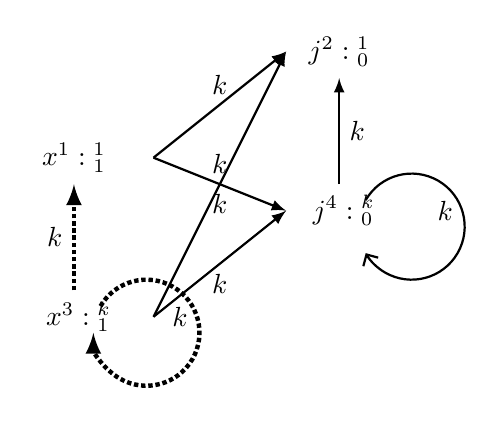
\begin{tikzpicture}[scale=\textwidth/18cm,samples=200]
  \draw[] (0, 7) circle (0pt) node
  {\textbf{$x^1: {}^{1}_{1}$}};
  \draw[] (0, 4) circle (0pt) node
  {{ $x^3: {}^{k}_{1}$}};
  % Counter Variables
  \draw[] (5, 9) circle (0pt) node {{$j^2: {}^{1}_{0}$}};
  \draw[] (5, 6) circle (0pt) node {{ $j^4: {}^{k}_{0}$}};
  %
  % Value Dependency Edges:
  \draw[ ultra thick, -latex, densely dotted,] (0, 4.5)  -- node[left]{\highlight{$k$}} (0, 6.5) ;
  \draw[ ultra thick, -latex, densely dotted,] (0.5, 4.2) arc (150:-180:1);
  \draw[] (2, 4) node []{\highlight{$k$}};
  \draw[ thick, -Straight Barb] (5.5, 6.2) arc (150:-150:1);
  \draw[] (7, 6) node []{\highlight{$k$}};
  \draw[ thick, -latex] (5, 6.5)  -- node[right]{\highlight{$k$}} (5, 8.5) ;
  % Control Dependency
  \draw[ thick,-latex] (1.5, 7)  -- node[above]{\highlight{$k$}} (4, 9) ;
  \draw[ thick,-latex] (1.5, 4)  -- node[above]{\highlight{$k$}} (4, 9) ;
  \draw[ thick,-latex] (1.5, 7)  -- node[below]{\highlight{$k$}} (4, 6) ;
  \draw[ thick,-latex] (1.5, 4)  -- node[below]{\highlight{$k$}} (4, 6) ;
  \end{tikzpicture}
  \caption{}
    \end{centering}
    \end{subfigure}
  }
   \caption{(a) Simple While Loop Example, (b) The Program-Based Dependency Graph generated from $\THESYSTEM$.}
  \label{fig:alg_adaptsearch_simplewhile}
  \end{figure}
  % \begin{figure}
% \centering
% {
% % \footnotesize
% \begin{subfigure}{.25\textwidth}
% \begin{centering}
% $ 
% \begin{array}{l}
%   \kw{whileSim(k)} \triangleq \\
%   \clabel{ \assign{j}{k} }^{0} ; \\
%   \clabel{ \assign{x}{\query(\chi[0])} }^{1} ; \\
%       \ewhile ~ \clabel{j > 0}^{2} ~ \edo ~ \\
%       \Big(
%        \clabel{\assign{x}{\query(\chi[x]) }}^{3}  ; \\
%       \clabel{\assign{j}{j-1}}^{4}       \Big)
%   \end{array}
% $
% \caption{}
% \end{centering}
% \end{subfigure}
% \quad
%   \begin{subfigure}{.6\textwidth}
%   \begin{centering}
%   \begin{tikzpicture}[scale=\textwidth/18cm,samples=200]
% \draw[] (0, 7) circle (0pt) node
% {\textbf{$x^1: {}^{1}_{1}$}};
% \draw[] (0, 4) circle (0pt) node
% {{ $x^3: {}^{k}_{1}$}};
% % Counter Variables
% \draw[] (5, 9) circle (0pt) node {{$j^2: {}^{1}_{0}$}};
% \draw[] (5, 6) circle (0pt) node {{ $j^4: {}^{k}_{0}$}};
% %
% % Value Dependency Edges:
% \draw[ ultra thick, -latex, densely dotted,] (0, 4.5)  -- (0, 6.5) ;
% \draw[ ultra thick, -latex, densely dotted,] (0.5, 4.2) arc (150:-180:1);
% \draw[ thick, -Straight Barb] (5.5, 6.2) arc (150:-150:1);
% \draw[ thick, -latex] (5, 6.5)  -- (5, 8.5) ;
% % Control Dependency
% \draw[ thick,-latex] (1.5, 7)  -- (4, 9) ;
% \draw[ thick,-latex] (1.5, 4)  -- (4, 9) ;
% \draw[ thick,-latex] (1.5, 7)  -- (4, 6) ;
% \draw[ thick,-latex] (1.5, 4)  -- (4, 6) ;
% \end{tikzpicture}
% \caption{}
%   \end{centering}
%   \end{subfigure}
% }
% % \end{wrapfigure}
% % \end{equation*}
% \vspace{-0.4cm}
%  \caption{(a) Simple While Loop Example, (b) The Program-Based Dependency Graph generated from $\THESYSTEM$.}
% \label{fig:alg_adaptsearch_simplewhile}
% \vspace{-0.5cm}
% \end{figure}
% Analysis Results: $ \progA(\kw{whileRec}(k)) = 1 + k$
%
If we traverse on the program-based dependency graph, and decrease the weight of $x^3$ (the weight $k$ is symbolic) by one after every visit,
% We can simply adopt either a deep first strategy to estimate the adaptivity as the length of the longest weight path, as 
% in Algorithm~\ref{alg:overadp_alg}.
we will never terminate because we only know $k \in \mathbb{N}$.

To solve this non-termination challenge, we switch to another walk finding approach: we first find a  longest path in the program-based dependency graph and then approximate the walk with the path.
Through a simple deep first search algorithm, we find the longest weighted path as the dotted arrow in Figure~\ref{fig:alg_adaptsearch_simplewhile},
$x^3: {}^k_1 \to x^1: {}^1_1 $.
Then, by summing up the weights on this path where the vertices has query annotation $1$, deep first search algorithm gives the adaptivity bound $1 + k$.
This is a the tight bound for this program's adaptivity.
% Look at the two-round example in overview, 
% it is easy to find that the longest weighted path is  $x^3 : {}^{k}_{1} \to a^5 : {}^{k}_{0} \to l^6 : {}^{1}_{0}$ with weighted query length $1 + k$.
% If we use this path to approximate a finite walk, and weight of each vertex as
% %  their visiting times, 
% its visiting time,
% then it isn't a qualified walk. 
% In the approximated walk, we have the vertices as $x^3 \to \cdots \to x^3 \to a^5 \to \cdots \to a^5 \to l^6$.

% However, this gives us over-approximation to a large extend in other cases as in \textbf{Approximation Challenge}.
% In Algorithm~\ref{alg:adpt_alg}, 
% we first find all the strong connected components of this graph, 
\textbf{Approximation Challenge:}
% As in Definition~\ref{def:finitewalk}, w
When we adopt a deep first strategy to search for the longest weighted path, and then use the path to approximate the adaptivity. We find that this gives us over-approximation to a large extend.
% Specifically, according to the finite walk definition in Definition~\ref{def:finitewalk},
% the visiting time of every vertex on a walk should be no more than its weight.
% However, by searching for the longest weighted path, 
% % and approximating the finite walk by this weight path, 
% and use it as the approximated finite walk with the longest query length, 
% the visiting times of the vertex on 
% % it 
% this approximated walk could 
% % possibly 
% exceed 
% % its weights. 
% the visiting times it can have.
% Then, this approximated walk isn't a qualified walk by Definition~\ref{def:finitewalk}, 
% and the weighted query length of this path is obviously greater than the maximum query length of the finite walk.
This over-approximation could result in a $\infty$ adaptivity upper bound on the program with actual adaptivity $2$.
Look at the two-round example in overview, 
it is easy to find that the longest weighted path is  $x^3 : {}^{k}_{1} \to a^5 : {}^{k}_{0} \to l^6 : {}^{1}_{0}$ with weighted query length $1 + k$.
If we use this path to approximate a finite walk, and weight of each vertex as
%  their visiting times, 
its visiting time,
then it isn't a qualified walk. 
In the approximated walk, we have the vertices as $x^3 \to \cdots \to x^3 \to a^5 \to \cdots \to a^5 \to l^6$.
Because $l^6$ can only be visited as most once by its weight,
% and this lead to 
resulting in the restriction on the maximum visiting time of $x^3$,
such that $x^3$ is only able to be visited at most once as well.
%
However, $x^3$ is visited $k$ times in this approximated walk.
% Moever, with the longest query length, then 
In order to have $x^3$ be visited $k$ time, we need to go back to 
$x^3$ on this walk from either $a^5$ or $l^6$ for $k$ time.
This is impossible since there is no edge going back to $x^3$ in $\progG(twoRound)$.
Obviously,
% the with the weighted length $1 + k$. It is obviously
its weighted query length, $1 + k$, 
% which is 
over approximates 
% its 
the adaptivity of this example to a large extend, which supposed to be $2$. 
%  for this program, 
% that 


These challenges motivate us to design a walk search algorithm through a combination of 
% DFS and BFS algorithm 
deep first search and breath first search strategy. 
% \wq{
This walk search algorithm consists of two components:
the path searching algorithm, $\pathsearch$ (in Algorithm~\ref{alg:adpt_alg})
which search for a 'suitable' path relying on the strong connected components of the program based dependency graph, 
and $\kw{\pathsearch_{scc}(G)}$ (in Algorithm~\ref{alg:adaptscc}) which approximates the
path.
% path found by Algorithm~\ref{alg:adpt_alg} 
% to a precise walk on the SCC
% and computes the adaptivity.
% These challenges give us the necessary to design a walk search algorithm through a combination of 
% % DFS and BFS algorithm 
% deep first search and breath first search strategy
% % as defined 
% as in Algorithm~\ref{alg:adpt_alg} and Algorithm~\ref{alg:adaptscc}.
%
The $\pathsearch$ as shown in Appendix Algorithm~I, takes our program-based dependency graph as input, and outputs the estimated adaptivity by two steps. 1. Process the input graph to a simplified graph 2. Perform
     the standard breath first search strategy to find the longest weighted path on this simplified graph and return the length as adaptivity.
The step 2 is not interesting, we now discuss step 1. 
The input dependency graph may contain circle due to the while loop, we simplify (shrank) the input graph by replacing every strong connected components(circle) of the graph with, the vertex whose weight is the adaptivity of the SCC 
(a subgraph of the input one) calculated by the $\pathsearch_{\kw{scc}}$. 
The SCC is found by using the Kosaraju's algorithm.
% \wq{cite}. 
The details of this algorithm is explained as follows.
    % This algorithm first finds all the strong connected components (SCC) of $\progG(c)$ using the Kosaraju’s algorithm in line:3. 
    % Every $\kw{SCC_1}, \cdots, \kw{SCC_n}$
    % where $0 \leq n \leq |\vertxs|$ is a sub-graph of $\progG(c)$, where $\kw{SCC_i} = (\vertxs_i, \edges_i, \weights_i, \qflag_i)$.
    % % where $\kw{SCC_i} = (\vertxs_i, \edges_i, \weights_i, \qflag_i)$.
    % Then, 
    % % we compute the adaptivity on every SCC, which is a subgraph of the $\progG(c)$, in line:4-5 by Algorithm~\ref{alg:adaptscc}.
    % it computes the adaptivity on every SCC
    % % , which is a subgraph of the $\progG(c)$, 
    % in line:4-5 by Algorithm~\ref{alg:adaptscc}.
    % % We guarantee the soundness of the adaptivity on SCC by Lemma~\ref{lem:sound_adaptalg_scc} with proof 
    % in Appendix.
    % % ~\ref{apdx:adaptalg_soundness}.
    % The $\progG(c)$ is then shrunk into an acyclic directed graph where 
    % % vertices are all the SCCs and edges are between every SCCs with their adaptivities as weights.
    % $\kw{SCC_1}, \cdots, \kw{SCC_n}$ are vertices with their adaptivities as weights.
    % % , and directed edges are .
    % For every $(v_i, v_j) \in \edges$ such that $v_1 \in \vertxs_i$, $v_j \in \vertxs_j$ and $i \neq j$,
    % there is a edge $(s_i, s_j)$ in this shrank graph. \\ 
    % Then, we use the standard breath first search strategy to find the longest weighted path
    % %  w.r.t. all the SCCs and their adaptivities.
    % on this shrank graph and return the length as adaptivity.
    % \\
%     We guarantee that 
%     % this longest weighted path is a sound computation of the adaptivity on this,
%     the length of this longest weighted path is a sound computation of the adaptivity for program $c$,
%     % as well as 
%     and this longest weighted path a sound computation of the finite walk having the longest query length 
%     % on this graph, in Theorem~\ref{thm:sound_adaptalg}
%     on $c$'s program based dependency graph, in Theorem~\ref{thm:sound_adaptalg}
%     in Appendix.
%     % ~\ref{apdx:adaptalg_soundness}.
% %    
% % \todo{add proof} 
% We also guarantee the conditional completeness of the adaptivity computation for graphs under the case that 
% $c$'s Program-Based Dependency Graph $\progG(c)$ is acyclic directed
% in Theorem~\ref{thm:adaptalg_pcomplete} 
% in Appendix~\ref{apdx:adaptalg_completeness}.
%
\paragraph*{The Adaptivity Computation Algorithm ($\pathsearch$)}
\begin{algorithm}
    \caption{
    {Adaptivity Computation Algorithm ($\pathsearch$)}
    \label{alg:adpt_alg}
    }
    \begin{algorithmic}[1]
    \REQUIRE $G = (\vertxs, \edges, \weights, \qflag)$ \#\{The program based dependency graph\}
    % with a start vertex $s$ and destination vertex $t$ .
    \STATE  {\bf {$\kw{\pathsearch(G)}$}:}  
    \STATE {\bf init} 
    % \\
    % current node: $c$, 
    \\
    $q$: empty queue.
    % \\
    % $\kw{visited}$: List of length $|\vertxs|$, initialize with $\efalse$.
    % \\
    % $\kw{SSCvisited}$: List of length $|\vertxs|$, initialize with $\efalse$.
    % \\ 
    % $\kw{adapt_{scc}(SCC_i) = \pathsearch_{scc}(SCC_i)}$.
    \\
    $\kw{adapt}$ : the adaptivity of this graph initialize with $0$.
    \\
    \STATE Find all Strong Connected Components (SCC) in $G$: $\kw{SCC_1}, \cdots, \kw{SCC_n}, 0 \leq n \leq |\vertxs|$, 
    % where $\kw{SCC_i} = (\vertxs_i, \edges_i, \weights_i, \qflag_i)$.
    % and assign each vertex $x^i$ with an SCC number $\kw{SCC}(x^i)$
    \STATE {\bf for} every SCC: $\kw{SCC_i}$, compute its Adaptivity $\kw{SCC_i}$:
    \STATE \quad $\kw{adapt_{scc}[SCC_i] = \pathsearch_{scc}(SCC_i)}$;
    \STATE {\bf for} every $\kw{SCC_i}$:
    \STATE \qquad $q.append(\kw{SCC_i})$;
    \STATE \qquad $\kw{adapt_{tmp}} = 0$;
    \STATE \qquad {\bf while} $q$ isn't empty:
    \STATE \qquad \qquad $\kw{s} = q.pop()$;  \#\{take the top SCC from head of queue\}
    \STATE \qquad \qquad  $\kw{adapt_{tmp}}_0= \kw{adapt_{tmp}}$; \#\{record the adaptivity of last level\}
    \STATE \qquad \qquad  $\kw{SCC_{max}}$;  \#\{record the SCC with longest walk in this level\}
    % initialize cycle-adapt = 0.
    \STATE \qquad \qquad {\bf for} every 
    % SCC having a directed edge from $s$ of $s$: $\kw{SCC'}$:
    % directed edge goes out of $\kw{s}$ and connects a 
    different SCC, $\kw{s'}$ connected by $\kw{s}$ by a directed edge from $\kw{s}$:
    % \STATE \qquad \qquad   cycle-adapt$ = \max($cycle-adapt, $\kw{dfs_{refine}(G, v, v)})$;
    % \STATE \qquad \qquad \qquad \#\{compute the adaptivity of vertex $v$  on $\kw{SCC}(v)$, and update r[v] with the SCC-adapt\}
    % \STATE \qquad \qquad \qquad $ r[v] = r[s] + \kw{dfs_{refine}(G, v, visited)})$; 
    \STATE \qquad \qquad \qquad {\bf if} $(\kw{adapt_{tmp}} < \kw{adapt_{tmp}}_0 + \kw{adapt_{scc}[s']})$:
    \STATE \qquad \qquad \qquad \qquad $\kw{adapt_{tmp}} = \kw{adapt_{tmp}}_0 + \kw{adapt_{scc}[s']}$; 
    \STATE \qquad \qquad \qquad \qquad $\kw{SCC_{max} = s'} $; \#\{update the SCC with longest walk in this level\} 
    % \STATE \qquad   $r[c] = r[c] + $cycle-adapt;
    % \STATE \qquad for all unvisited vertex $v$ having directed edge from c and $! \kw{cycle}(c)$:
    % \STATE \qquad \qquad $r[v] = r[c] + \flag(v)$; 
    % \STATE \qquad \qquad \qquad  \#\{mark all the nodes with the same $\kw{SCC}$ number as visited\} 
    % \STATE \qquad \qquad \qquad  \#\{append the unvisited vertex to the rear of the queue\}
    % \STATE \qquad \qquad \qquad  \#\{mark all the nodes with the same $\kw{SCC}$ number as visited\} 
    % \STATE \qquad \qquad for $v \in V$,   $\kw{visited}[s] = 1$;
    \STATE \qquad \qquad \qquad $q.append(\kw{SCC_{max}})$;
    \STATE \qquad $\kw{adapt} = \max(\kw{adapt}, \kw{adapt_{tmp}})$;    
    \RETURN $\kw{adapt}$.
    \end{algorithmic}
    \end{algorithm}
    %
%
    % In Algorithm~\ref{alg:adpt_alg}, 
    % it 
    This algorithm first finds all the strong connected components (SCC) of $\progG(c)$ using the Kosaraju’s algorithm in line:3.
    Every $\kw{SCC_1}, \cdots, \kw{SCC_n}$
    where $0 \leq n \leq |\vertxs|$ is a sub-graph of $\progG(c)$, where $\kw{SCC_i} = (\vertxs_i, \edges_i, \weights_i, \qflag_i)$.
    % where $\kw{SCC_i} = (\vertxs_i, \edges_i, \weights_i, \qflag_i)$.
    Then, 
    % we compute the adaptivity on every SCC, which is a subgraph of the $\progG(c)$, in line:4-5 by Algorithm~\ref{alg:adaptscc}.
    it computes the adaptivity on every SCC
    % , which is a subgraph of the $\progG(c)$, 
    in line:4-5 by Algorithm~\ref{alg:adaptscc}.
    We guarantee the soundness of the adaptivity on SCC by Lemma~\ref{lem:sound_adaptalg_scc} with proof in Appendix~\ref{apdx:adaptalg_soundness}.
    The $\progG(c)$ is then shrunk into an acyclic directed graph where 
    % vertices are all the SCCs and edges are between every SCCs with their adaptivities as weights.
    $\kw{SCC_1}, \cdots, \kw{SCC_n}$ are vertices with their adaptivities as weights.
    % , and directed edges are .
    For every $(v_i, v_j) \in \edges$ such that $v_1 \in \vertxs_i$, $v_j \in \vertxs_j$ and $i \neq j$,
    there is a edge $(s_i, s_j)$ in this shrank graph. \\ 
    Then, we use the standard breath first search strategy to find the longest weighted path
    %  w.r.t. all the SCCs and their adaptivities.
    on this shrank graph and return the length as adaptivity.
    \\
    We guarantee that 
    % this longest weighted path is a sound computation of the adaptivity on this,
    the length of this longest weighted path is a sound computation of the adaptivity for program $c$,
    % as well as 
    and this longest weighted path a sound computation of the finite walk having the longest query length 
    % on this graph, in Theorem~\ref{thm:sound_adaptalg}
    on $c$'s program based dependency graph, in Theorem~\ref{thm:sound_adaptalg}
    in Appendix.
    % ~\ref{apdx:adaptalg_soundness}.
%    
% \todo{add proof} 
We also guarantee the conditional completeness of the adaptivity computation for graphs under the case that 
$c$'s Program-Based Dependency Graph $\progG(c)$ is acyclic directed
in Theorem~\ref{thm:adaptalg_pcomplete} 
in Appendix~\ref{apdx:adaptalg_completeness}.
    % for every vertex which isn't on any SCC, it is easy to know that it will be visited 
    % at most once given no edges going back to this vertex. We can know the adaptivity on the SCC 
     %
    % \begin{algorithm}
    % \caption{
    % {Longest Adaptivity Search Algorithm ($\pathsearch$)}
    % \label{alg:adpt_alg}
    % }
    % \begin{algorithmic}
    % \REQUIRE Weighted Directed Graph $G = (\vertxs, \edges, \weights, \flag)$ with a start vertex $s$ and destination vertex $t$ .
    % \STATE  {\bf {bfs $(G)$}:}  
    % \STATE {\bf init} 
    % \\
    % current node: $c$, 
    % \\
    % queue: $q$ : List, add into $a$ an arbitrary v from $\vertxs$. 
    % \\
    % visited: List of length $|\vertxs|$, initialize with $\efalse$.
    % \\
    % results: $r$ : List of length $|\vertxs|$, initialize with -1.
    % \\
    % curr$\kw{flowcapacity}$: INT, initialize MAXINT.
    % \\
    % querynum: INT, initialize 0. \#\{To count the query numbers when we are walking inside a cycle\}
    % \\
    % \STATE \qquad {\bf while} $q$ isn't empty:
    % \STATE \qquad \qquad take the vertex from head $c= q.pop()$
    % \STATE \qquad \qquad mark $c$ as visited, visited $[c] = 1$.
    % \STATE \qquad \qquad {\bf if} $\kw{cycle}(c)$  \#\{we are inside a cycle\}
    % \STATE \qquad \qquad \qquad curr$\kw{flowcapacity}$ = min($\weights$(c), curr$\kw{flowcapacity}$).
    % \STATE \qquad \qquad \qquad querynum += $\flag(c)$.
    % \STATE \qquad \qquad  \qquad for all unvisited vertex $v$ having directed edge from c:
    % \STATE \qquad \qquad \qquad \qquad r[v] = r[c]; q.add(v)
    % \STATE \qquad \qquad \qquad  {\bf if}  $v$ is visited, then the circle finished
    % \STATE \qquad \qquad \qquad \qquad update the result $r[v] =  \max(r[v], r[c] + $curr$\kw{flowcapacity}$*querynum)
    % \STATE \qquad \qquad \qquad \qquad curr$\kw{flowcapacity}$ = MAXINT
    % \STATE \qquad \qquad \qquad \qquad querynum = 0.  
    % \STATE \qquad \qquad {\bf else} 
    % \STATE \qquad \qquad \qquad for all unvisited vertex $v$ having directed edge from c:
    % \STATE \qquad \qquad \qquad  \qquad $r[v] = \max(r[v], r[c] + \flag(c))$; q.add(v)
    % \RETURN max($r$)
    % \end{algorithmic}
    % \end{algorithm}
    %
%
    % \begin{algorithm}
    %     \caption{
    %     {Over-Approximated Adaptivity on SCC}
    %     \label{alg:overadp_alg}
    %     }
    %     \begin{algorithmic}
    %     \REQUIRE Weighted Directed Graph $G = (\vertxs, \edges, \weights, \qflag)$ with a start vertex $s$ and destination vertex $t$ .
    %     \STATE  {\bf {$\kw{dfs_{naive}(G, c,visited)}$}:}  
    %     % \STATE {\bf init} 
    %     % \\
    %     % current node: $c$, 
    %     % \\
    %     % visited: List of length $|\vertxs|$, initialize with $\efalse$.
    %     % \\
    %     % \STATE {\bf if} $c = s$:
    %     % \RETURN \qquad  $\weights(s)*\flag(s) $.
    %     \STATE $r[c] = \weights(c)*\qflag(c) $
    %     \STATE {\bf for}  all vertex $v$ having directed edge from $c$:
    %     \STATE \qquad {\bf if}  $v$ is unvisited:
    %     \STATE \qquad \qquad  \#\{mark $v$ as visited\} $\kw{visited}[v] = 1$;
    %     \STATE \qquad \qquad $r[c] += \kw{dfs_{naive}(G, v, visited)}$;
    %     % \STATE \qquad {\bf else}: \#\{There is a cycle finished\}
    %     % \RETURN \qquad \qquad $\weights(v)*\flag(v) $.
    %     \RETURN $r[c]$
    %     \end{algorithmic}
    %     \end{algorithm}%
        %
  \paragraph*{Adaptivity Computation Algorithm on SCC Graph ($\kw{\pathsearch_{scc}(G)}$)}
    \begin{algorithm}
            \caption{
            {Adaptivity Computation Algorithm on SCC Graph }
            \label{alg:adaptscc}
            }
            \begin{algorithmic}[1]
              \REQUIRE $G = (\vertxs, \edges, \weights, \qflag)$ \#\{An Strong Connected program based dependency Graph\}
            \STATE  {\bf {$\kw{\pathsearch_{scc}(G)}$}:}  
            \STATE {\bf init} 
            \\
            $\kw{r_{scc}}$: $EXPR(\constdom)$, initialized $0$, the Adaptivity of this SCC
            \STATE \qquad {\bf init} 
            % \STATE \qquad current node: $c$, 
            % \\
            % visited: List of length $|\vertxs|$, initialize with $\efalse$.
            % \\ \qquad  $\kw{r_{scc}}$ : initialize $0$, the adaptivity of this graph
            \\ \qquad  $\kw{visited}$ : $\{0, 1\}$ List, 
            \\ \qquad  \#\{length $|\vertxs|$, initialize with $0$ for every vertex, recording whether a vertex is visted.\}
            \\ \qquad  $\kw{r}$ : $EXPR(\constdom)$ List, 
            \\ \qquad  \#\{length $|\vertxs|$, initialize with $\qflag(v)$ for every vertex, recording the adaptivity reaching each vertex.\}
            \\ \qquad  $\kw{flowcapacity}$: $EXPR(\constdom)$ List, 
            % INT List of length $|\vertxs|$, initialize MAXINT. 
            \\ \qquad  \#\{length $|\vertxs|$, initialize with $\infty$ for every vertex,
            % \#\{For every vertex, 
            recording the minimum weight when the walk reaching 
            that vertex, inside a cycle\}
            \\ \qquad  $\kw{querynum}$: INT List,
            %  of length $|\vertxs|$, initialize with $\qflag(v)$ for every vertex. 
            \\ \qquad  \#\{length $|\vertxs|$, initialize with $\qflag(v)$ for every vertex, 
            % \#\{For every vertex, 
            recording the query numbers when the path reaching 
            that vertex, inside a cycle\}
            \STATE {\bf if} $|\vertxs| = 1$ and $|\edges| = 0$:
            \STATE \qquad {\bf return}  $\qflag(v)$
            \STATE  {\bf def} {$\kw{dfs(G, c,visited)}$}:
            % \STATE \qquad update the length of the longest path reaching this vertex
            % $r[s] =  r[s] + $$\kw{flowcapacity}$[s] * querynum[s].
            % \RETURN  \qquad $r[s]$.      
            \STATE \qquad {\bf for} every vertex $v$ 
            % having directed edge from $c$:
            connected by a directed edge from $c$:
            \STATE \qquad \qquad {\bf if} $\kw{visited}[v] = \efalse$:
            \STATE \qquad \qquad \qquad $\kw{flowcapacity[v] = \min(\weights(v), {flowcapacity}[c])}$;
            \STATE \qquad \qquad \qquad $\kw{querynum[v] = querynum[c] + \qflag(v)}$;
            % \STATE \qquad \qquad \qquad \#\{do not update the length of the longest walk reaching $v$ until the cycle is finished\}
            % \STATE \qquad \qquad \qquad $\kw{r[v] =  r[c] + flowcapacity[v] \times querynum[v]} $; \#\{do not update the length of the longest walk reaching $v$ until the cycle is finished\}
            \STATE \qquad \qquad \qquad $\kw{r[v] =  \max(r[v], flowcapacity[v] \times querynum[v]}) $; 
            % \#\{do not update the length of the longest walk reaching $v$ until the cycle is finished\}
            \STATE \qquad \qquad \qquad  $\kw{visited}[v] = 1$; %\#\{mark $v$ as visited\}
            \STATE \qquad \qquad \qquad $\kw{dfs(G, v, visited)}$;
            \STATE \qquad \qquad {\bf else}: \#\{There is a cycle finished\}
            % \STATE \qquad \qquad \qquad \#\{update the length of the longest path reaching this vertex\}
            \STATE \qquad \qquad \qquad 
            $\kw{r[v] =  \max(r[v], r[c] +  \min(\weights(v), {flowcapacity}[c]) * (querynum[c] + \qflag(v)))}$; \#\{update the length of the longest walk reaching this vertex on this cycle\}
            %  $\kw{r[v] =  \max(r[v], r[c] + flowcapacity[v] * querynum[v])}$; \#\{update the length of the longest walk reaching this vertex on this cycle\}
            %  \STATE \qquad \qquad \qquad \#\{Recover the $\kw{flowcapacity}$ and querynumber to previous state, for different loops\}
            % \STATE \qquad \qquad \qquad $\kw{flowcapacity[v] = flowcapacity[c]}$; \#\{Recover the $\kw{flowcapacity}$\}
            % \STATE \qquad \qquad \qquad $\kw{querynum[v] = querynum[c]}$;\#\{Recover the $\kw{querynum}$\}
            \STATE \qquad {\bf return}  $\kw{r[c]}$
            \STATE  {\bf for} every vertex $v$ in $\vertxs$:
            \STATE  \qquad initialize the $\kw{visited, r, flowcapacity, querynum}$;
            \STATE  \qquad $\kw{r_{scc} = \max(r_{scc}, dfs(G, v, \kw{visited} ))}$ ; 
            \RETURN  $\kw{r_{scc}}$
            \end{algorithmic}
            \end{algorithm}
            % \\
% Following is the challenge of computing the adaptivity on a program based dependency graph.
% In order to search for the finite walk having the longest query length, which isn't a simple longest weighted path.
% \\
% the visiting times of every vertex on this walk should be no more than its weight, which is a symbolic expression.
% So we cannot simply search for the longest weight path where the visiting times of the vertex on it could possibly exceed its weights.
% We can neither simply traverse on this graph by decreasing the weight of every node by 1 after every visiting,
% because the weight is symbolic and simply traversing leads to non-termination.
% \\
% In Algorithm~\ref{alg:adaptscc}, 
This algorithm takes a subgraph of the program-based dependency graph as input, to be precise, the input graph is SCC, and the output is the adaptivity of this SCC. 
For an SCC containing only one vertex without any edge, it returns the query annotation of this vertex as adaptivity.
For SCC containing at least one edge, 
There are three steps in this algorithm: 1. find out all the paths in the input SCC 2. Calculate the adaptivity of every path using our designed adaptivity counting method. 3. Return the maximal adaptivity among all the paths. The step 3 is trivial. Because our input graph is SCC, when we start traversing from a vertex, we will finally go back to this vertex. The paths we find in step 1 are all those with the same starting and ending vertex. The most interesting part is step 2. 
We discuss as follows.

This algorithm first check if an SCC contains only one vertex without any edge, as in line:4-5 in Algorithm~\ref{alg:adaptscc}.
% then 
% \\
% If yes, then it's easy to know that it will be visited 
% at most once since there isn't edge going back to this vertex. 
% So we can know that the adaptivity on this SCC is at most one if it is a query vertex,
% and zero otherwise.
% \\
% If not, then 
Again, for 
the SCC containing only one vertex without any edge, as in line:4-5 in Algorithm~\ref{alg:adaptscc}.
% then 
% If yes, then i
% it's easy to know that it will be visited 
% at most once since there isn't edge going back to this vertex. 
% So we can know 
The adaptivity on this SCC is at most one if it is a query vertex,
and zero otherwise.
$\kw{\pathsearch_{scc}(G)}$ return query annotation directly as in line:4-5.
% So $\kw{\pathsearch_{scc}(G)}$ return query annotation directly as in line:4-5.
\\
% For the SCC contains at least one edge, we are searching for the finite walk having the longest query length through a deep first search strategy.
For the SCC containing at least one edge, 
we compute the adaptivity for each path 
on the fly of searching for the paths 
in the
% design a 
recursion algorithm $\kw{dfs}$ designed based on 
a deep first search strategy 
% of this algorithm is described as follows,
from line: 6-16 in $\kw{\pathsearch_{scc}(G)}$ in Algorithm~\ref{alg:adaptscc}.
\\
% The difficulty is, the visiting times of every vertex on this walk should be no more than its weight, which is a symbolic expression.
% As the two challenges discussed above, we want to guarantee the visiting time of each vertex smaller than 
% its weight, in the meantime the algorithm termination. 
% Additionally, we are computing the query length rather than sum of the weights.
% We design a deep first search strategy
% % of this algorithm is described as follows,
% from line: 6-16 in Algorithm~\ref{alg:adaptscc}, 
% searching for the finite walk having the longest query length
% %  through a deep first search strategy
% with a capacity limitation and use special parameter to compute the adaptivity.
%
As the \textbf{Approximation Challenge} discussed above, 
we want to guarantee the visiting time of each vertex smaller than 
its weight and compute the adaptivity accurately, in the meantime guarantee the algorithm termination. 
It uses a capacity limitation and  special parameters to achieve it,
specifically as follows.
Additionally, we are computing the query length rather than sum of the weights.
We design a deep first search strategy
% of this algorithm is described as follows,
from line: 6-16 in Algorithm~\ref{alg:adaptscc}, 
% searching for the finite walk having the longest query length
%  through a deep first search strategy
with a capacity limitation and use special parameter to compute the adaptivity.
% for every path.
%
% for every path.
% So we cannot simply search for the longest weight path where the visiting times of the vertex on it could possibly exceed its weights.
% We can neither simply traverse on this graph by decreasing the weight of every node by 1 after every visiting,
% because the weight is symbolic and simply traversing leads to non-termination.
% \\
\\
In order to
guarantee the termination, 
% this algorithm 
$\kw{\pathsearch_{scc}(G)}$
terminates the recursion if monitored a cycle, as in line:8 and line:14, through a boolean list $\kw{visited}$.
This guaranteed the termination and solved the \textbf{Challenge II.} discussed above.
% \todo{solve the challenge 2} 
% search for finite walk  
% So we use the dfs to search for the 
\\
% In order to
% solve the \textbf{Challenge I},
% specifically guarantee the visiting times of each vertex by its weight, 
% we use a special parameter $\kw{flowcapacity}$  to track the minimum weight during the 
% % dfs process, 
% deep first searching along the walk, 
% also a parameter $\kw{querynum}$
% % to compute the query length of this walk
% to track the total number of vertices which are query vertices along the walk in order to compute the query length of this walk.
In order to
solve the \textbf{Approximation Challenge},
specifically guarantee the visiting times of each vertex by its weight
and compute the adaptivity accurately, 
we use a special parameter $\kw{flowcapacity}$  to track the minimum weight
along the path during the 
% dfs process, 
% deep first 
searching procedure, 
and a parameter $\kw{querynum}$
% to compute the query length of this walk
to track the total number of vertices with query annotation $1$
% which are query vertices 
along the path 
in order to compute the query length.
% 
% \todo{solve the challenge 1, specifically in the dfs strategy
% of this algorithm is described as follows,
% from line: 6-16 in Algorithm~\ref{alg:adaptscc}. } 
% \\
% Then, to compute the query length of this walk, 
% we use another parameter $\kw{querynum}$
% to track the total number of vertices which are query vertices along the walk.

The detail steps of this dfs strategy
% of this algorithm is described as follows,
from line: 3-16 in Algorithm~\ref{alg:adaptscc},
particularly from line: 7-15 on how to 
use these two special parameters to resolve \textbf{Approximation Challenge}
 is described as follows.
 %
 $\kw{flowcapacity}$ is a list of symbolic expressions for every vertex, recording the minimum weight when the path reaches that vertex, which is initialized by $\infty$.
% , inside a cycle\}

$\kw{querynum}$ is a list of integer with length $|\vertxs|$, which is initialized with $\qflag(v)$ for every vertex. 
For every vertex, 
% recording the query numbers when the path reaching.
% in order to 
it records the total query numbers when the path reaching this vertex.

We maintain the minimum weight for the 
$\kw{flowcapacity}$, 
number of query vertices 
$\kw{querynum}$ 
and update the adaptivity for this path $\kw{r}$
alone the path and update the adaptivity reaching 
this vertex, 
when traversing on this graph, as in Algorithm~\ref{alg:adaptscc} from line: 8-13.
% and then recursively dfs on all vertices heading out from this vertex.
% \\
At line: 15 where this vertex is visited, i.e., this path 
going back to its starting node,
we only update the adaptivity $\kw{r}$ reaching this vertex.
% and neither recursion nor update the $\kw{flowcapacity}$  and 
% $\kw{querynum}$.
\\
% Again, Non-recursion in the second branch
% % in order to 
% guarantees the termination and resolves \textbf{Non-Termination Challenge}.
% \\
The updating operations
during the traversing 
(in line: 11) and 
at the end of the traverse (in line: 15),
% in these two branches, 
specifically the $\kw{flowcapacity[v] \times querynum[v]}$ 
% in line: 11 and line: 15 
computes the query length for this path. 
it guarantees 
the visiting times of each vertex on the path reaching a vertex $v$ is no more than 
the maximum visiting it can be on a qualified walk, through $\kw{flowcapacity[v]}$,
and in the same time  compute the query length instead of weighted length accurately through 
$\kw{ querynum[v]}$.
%  its minimum visiting time, 
In this way, we resolve the \textbf{Approximation Challenge} and in the same time without losing the soundness,
% searching for the finite walk having the longest query length through a deep first search strategy
% with a capacity limitation and use special parameter to compute the adaptivity
% for every path.
\\
We first initialize some parameters:
\\
$\kw{visited}$ is initialized as a list of $0$ for every vertex on this SCC, in order to guarantee the termination;
\\ 
$\kw{r}$ is initialized  as a list of integer with length $|\vertxs|$, initialize with $\qflag(v)$ for every vertex. The adaptivity reaching each vertex.
\\ 
$\kw{flowcapacity}$ a list of symbolic expressions for every vertex, recording the minimum weight when the walk reaching that vertex, which  is initialized by $\infty$.
% , inside a cycle\}
\\ 
$\kw{querynum}$ is a list of integer with length $|\vertxs|$, which is initialized with $\qflag(v)$ for every vertex. 
For every vertex, 
% recording the query numbers when the path reaching.
in order to record the total query numbers when the walk reaches a vertex.
\\
Then from line: 5-11, we record the minimum weight and number of query vertices alone the path and update the adaptivity reaching 
this vertex, and then recursively dfs on all vertices heading out from this vertex.
\\
At line: 12 where this vertex is visited, 
we only update the adaptivity reaching this vertex and neither recursion nor update the $\kw{flowcapacity}$  and 
$\kw{querynum}$.
% \\
% Again, Non-recursion in the second branch
% % in order to 
% guarantees the termination and resolves \textbf{Challenge I}.
\\
The updating operation in these two branches, 
specifically $\kw{flowcapacity[v] \times querynum[v]}$ in line: 11 and line: 15 
guarantees 
1.the visiting times of each vertex on the walk reaching $v$ is no more than 
the maximum visiting it can be on this walk, through $\kw{flowcapacity[v]}$. 
%  its minimum visiting time, 
In this way, we resolve the \textbf{Approximation Challenge}  and in the same time without losing the soundness 
% this 
% 2. then 
by using $\kw{flowcapacity[v] \times querynum[v]}$ to compute the query length. 
% without lose the adaptivity.
%
\\
Notice here, another special operation we have in the second branch is Non-updating of
% Non-updating the 
$\kw{querynum}$ and $\kw{flowcapacity}$.
This guarantees both the accuracy and the soundness, formally in Lemma~\ref{thm:sound_adaptalg} in Appendix~\ref{apdx:adaptalg_soundness}.

Now, we show an example illustrating how our two updating operations for adaptivity 
for each path can guarantee both the accuracy and the soundness. 
Look at a Nested While Loop example program in Figure~\ref{fig:alg_adaptsearch_nestedwhile}.
% Notice here, another special operation we have in the second branch is Non-updating of
% % Non-updating the 
% $\kw{querynum}$ and $\kw{flowcapacity}$.
% This guarantees both the accuracy and the soundness.
% Specifically,
% % because a second visiting of the same vertex 
% if this vertex is visited, it indicates that a cycle is monitored and  
% % indicates there is a cycle goes back to this vertex, 
% the traversing on this cycle is finished by going back to this vertex.
% %
% % then, when 
% When we continuously search for walks heading out of this vertex, 
% the minimum weight on this cycle does not affect the walks going out of this vertex that not pass this cycle.
% However, if we keep recording the minimum weight, then we
% %  are restricting 
% restrict the visiting times of vertices on a walk by
%  using the minimum weight of vertices not on this walk.
% %  , it is unsound anymore.
% Then, it is obviously that this leads to unsoundness.
% \todo{example} 
% To under stand how the two operations 
We first search for a path: $y^6 \to y^6$, and compute the adaptivity for this path as 
$k$.
Notice here, another special operation we have in the second branch is Non-updating of
% Non-updating the 
$\kw{querynum}$ and $\kw{flowcapacity}$.
This guarantees both the accuracy and the soundness.
Specifically,
% because a second visiting of the same vertex 
if this vertex is visited, it indicates that a cycle is monitored and  
% indicates there is a cycle goes back to this vertex, 
the traversing on this cycle is finished by going back to this vertex.
%
% then, when 
When we continuously search for walks heading out of this vertex, 
the minimum weight on this cycle does not affect the walks going out of this vertex that not pass this cycle.
However, if we keep recording the minimum weight, then we
%  are restricting 
restrict the visiting times of vertices on a walk by
using the minimum weight of vertices not on this walk.
%  , it is unsound anymore.
Then, it is obviously that this leads to unsoundness.
If we update the $\kw{flowcapacity}[y^6]$ as $k$ after visiting $y^6$ the second time 
on this walk,
% the walk $y^6 \to y^6$,
and continuously visit $x^9$,
then the $\kw{flowcapacity[k]}$ is 
updated as $\min(k, k^2)$.
So
%  which 
% restricting 
the visiting times of $x^9$ is restricted by $k$ on the walk $y^6 \to y^6 \to x^9$.
This restriction excludes the finite walk $y^6 \to y^6 \to x^9 \to x^9$ where $y^6$ and $x^9$ visited by $k^2$ times
in the computation. 
However, the finite walk $y^6 \to y^6 \to x^9 \to x^9$ where $y^6$ is visited $k$ times and $x^9$ $k^2$ times is 
a qualified walk, and exactly the longest walk we aim to find. So, by Non-updating the $\kw{flowcapacity}$ after 
visiting $y$ again, we guarantee that the visiting times og vertices on every searched walk will not be restricted by weights not on this walk,
i.e., the soundness.
\\
In the last line of this dfs algorithm, line: 16, it returns the adaptivity heading out from its input vertex.
\\
By applying this deep first search strategy on every vertex on this SCC, 
we compute the adaptivity of this SCC by taking the maximum 
% adaptivity reaching every vertex on this SCC.
value over every vertex.
%
The soundness is formally guaranteed in Lemma~\ref{lem:sound_adaptalg_scc} in Appendix~\ref{apdx:adaptalg_soundness}.

% Look at a Nested While Loop example program in Figure~\ref{fig:alg_adaptsearch_nestedwhile}.

% Specifically,
% % because a second visiting of the same vertex 
% if this vertex is visited, it indicates that a cycle is monitored and  
% % indicates there is a cycle goes back to this vertex, 
% the traversing on this cycle is finished by going back to this vertex.
% %
% % then, when 
% When we continuously search for walks heading out of this vertex, 
% the minimum weight on this cycle does not affect the walks going out of this vertex that not pass this cycle.
% However, if we keep recording the minimum weight, then we
% %  are restricting 
% restrict the visiting times of vertices on a walk by
%  using the minimum weight of vertices not on this walk.
% %  , it is unsound anymore.
% Then, it is obviously that this leads to unsoundness.
 %
  %
  \begin{figure}
    \centering
    {\footnotesize
    \begin{subfigure}{.4\textwidth}
    \begin{centering}
    % 
    $ 
    \begin{array}{l}
      \kw{nestedWhileMultiVarRecAcross}(k) \triangleq \\
      \clabel{\assign{i}{k} }^{0} ; \\
      \clabel{ \assign{x}{\query(\chi[0])}}^{1} ; \\
      \clabel{ \assign{y}{\query(\chi[1])}}^{2} ; \\
          \ewhile ~ \clabel{i > 0}^{3} ~ \edo ~ \\
          \Big(
           \clabel{\assign{i}{i-1}}^{4} ;\\
           \clabel{\assign{j}{k}}^{5} ;\\
           \clabel{\assign{y}{\query(\chi(\ln(x) + y))} }^{6}  ; \\
           \ewhile ~ \clabel{j > 0}^{7} ~ \edo ~ \\
           \Big(
            \clabel{\assign{j}{j-1}}^{8};\\
            \clabel{\assign{x}{\query(\chi(\ln(y))+\chi[x])} }^{9}
            \Big) \Big)
      \end{array}
    %       
    $
    \caption{}
    \end{centering}
    \end{subfigure}
    \quad
    \begin{subfigure}{.52\textwidth}
      \begin{centering}
      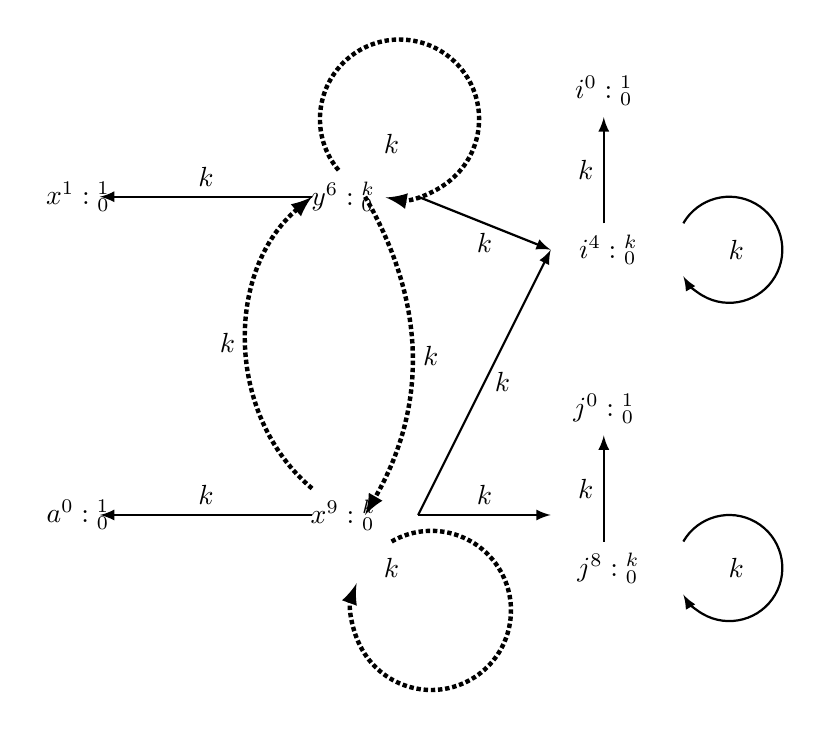
\begin{tikzpicture}[scale=\textwidth/18cm,samples=200]
      % Variables Initialization
      \draw[] (-5, 1) circle (0pt) node{{ $a^0: {}^1_{0}$}};
      \draw[] (-5, 7) circle (0pt) node{{ $x^1: {}^{1}_{0}$}};
      % Variables Inside the Loop
      \draw[] (0, 7) circle (0pt) node{{ $y^6: {}^{k}_{0}$}};
      \draw[] (0, 1) circle (0pt) node{{ $x^9: {}^{k}_{0}$}};
      % Counter Variables
      \draw[] (5, 9) circle (0pt) node {{$i^0: {}^{1}_{0}$}};
      \draw[] (5, 6) circle (0pt) node {{ $i^4: {}^{k}_{0}$}};
      \draw[] (5, 3) circle (0pt) node {{$j^0: {}^{1}_{0}$}};
      \draw[] (5, 0) circle (0pt) node {{ $j^8: {}^{k}_{0}$}};
      % Value Dependency Edges:
      \draw[ ultra thick, -latex, densely dotted,] (0, 7.5) arc (220:-100:1.5);
      \draw[] (1, 8) node [] {\highlight{$k$}};
      \draw[ thick, -latex] (5, 6.5)  -- node[left]{\highlight{{$k$}}}(5, 8.5) ;
      \draw[ thick, -latex] (5, 0.5)  -- node[left]{\highlight{{$k$}}}(5, 2.5) ;
      \draw[ ultra thick, -latex, densely dotted,] (1., 0.5) arc (120:-200:1.5);
      \draw[] (1, 0) node [] {\highlight{$k$}};
      % Value Dependency Edges on Initial Values:
      \draw[ thick, -latex,] (-0.5, 1)  -- node[above]{\highlight{{$k$}}}(-4.5, 1) ;
      \draw[ thick, -latex,] (-0.5, 7)  -- node[above]{\highlight{{$k$}}}(-4.5, 7) ;
      %
      \draw[ ultra thick, -latex, densely dotted,] (-0.5, 1.5)  to  [out=-220,in=220]  
      node[left]{\highlight{{$k$}}}(-0.5, 7);
      \draw[ ultra thick, -latex, densely dotted,]  (0.5, 7) to  [out=-60,in=60] 
      node[right]{\highlight{{$k$}}}(0.5, 1) ;
      % Control Dependency
      \draw[ thick, -latex, ] (6.5, 6.5) arc (150:-150:1);
      \draw[] (7.5, 6) node [] {\highlight{$k$}};
      \draw[ thick, -latex, ] (6.5, 0.5) arc (150:-150:1);
      \draw[] (7.5, 0) node [] {\highlight{$k$}};
      \draw[ thick,-latex] (1.5, 7)  -- node[below]{\highlight{{$k$}}}(4, 6) ;
      \draw[ thick,-latex] (1.5, 1)  -- node[right]{\highlight{{$k$}}}(4, 6) ;
      \draw[ thick,-latex] (1.5, 1)  -- node[above]{\highlight{{$k$}}}(4, 1) ;
   \end{tikzpicture}
   \caption{}
      \end{centering}
      \end{subfigure}
    }
     \caption{(a) Nested While Loop Example, (b) Execution-Based Dependency Graph, (c) The Static Program-Based Dependency graph.}
    \label{fig:alg_adaptsearch_nestedwhile}
    \vspace{-0.5cm}
    \end{figure}
    %
%     When we searched for a walk: $y^6 \to y^6$,
%   if we update the $\kw{flowcapacity}[y^6]$ as $k$ after visiting $y^6$ the second time 
%   on this walk,
%   % the walk $y^6 \to y^6$,
%   and continuously visit $x^9$,
%   then the $\kw{flowcapacity[k]}$ is 
%   updated as $\min(k, k^2)$.
%   So
%   %  which 
%   % restricting 
%   the visiting times of $x^9$ is restricted by $k$ on the walk $y^6 \to y^6 \to x^9$.
%   This restriction excludes the finite walk $y^6 \to y^6 \to x^9 \to x^9$ where $y^6$ and $x^9$ visited by $k^2$ times
%   in the computation. 
%   However, the finite walk $y^6 \to y^6 \to x^9 \to x^9$ where $y^6$ is visited $k$ times and $x^9$ $k^2$ times is 
%   a qualified walk, and exactly the longest walk we aim to find. So, by Non-updating the $\kw{flowcapacity}$ after 
%   visiting $y$ again, we guarantee that the visiting times og vertices on every searched walk will not be restricted by weights not on this walk,
%   i.e., the soundness.
%  \\
% In the last line of this dfs algorithm, line: 16, it returns the adaptivity heading out from its input vertex.
% \\
% By applying this deep first search strategy on every vertex on this SCC, 
% we compute the adaptivity of this SCC by taking the maximum 
% % adaptivity reaching every vertex on this SCC.
% value over every vertex.
% %
% The soundness is formally guaranteed in Lemma~\ref{lem:sound_adaptalg_scc} in Appendix~\ref{apdx:adaptalg_soundness}.
            % \begin{algorithm}
        % \caption{
        % {Refined Adaptivity on $\kw{SCC}$}
        % \label{alg:dfscycle_alg}
        % }
        % \begin{algorithmic}
        % \REQUIRE Weighted Directed Graph $G = (\vertxs, \edges, \weights, \qflag)$ with a start vertex $s$ and destination vertex $t$ .
        % \STATE  {\bf {$\kw{dfs_{refine}(G, c, visited)}$}:}  
        % \STATE {\bf init} 
        % \\
        % current node: $c$, 
        % % \\
        % % visited: List of length $|\vertxs|$, initialize with $\efalse$.
        % \\
        % results: $r$ : INT List of length $|\vertxs|$, initialize with $\qflag(v)$ for every vertex.
        % \\
        % $\kw{flowcapacity}$: INT List of length $|\vertxs|$, initialize MAXINT. 
        % \#\{For every vertex, recording the minimum weight when the walk reaching 
        % that vertex, inside a cycle\}
        % \\
        % querynum: INT List of length $|\vertxs|$, initialize with $\qflag(v)$ for every vertex. 
        % \#\{For every vertex, recording the query numbers when the walk reaching 
        % that vertex, inside a cycle\}
        % \\
        % % \STATE {\bf if} $c = s$:
        % % \STATE \qquad update the length of the longest path reaching this vertex
        % % $r[s] =  r[s] + $$\kw{flowcapacity}$[s] * querynum[s].
        % % \RETURN  \qquad $r[s]$.      
        % \STATE {\bf for}  all vertex $v$ having directed edge from $c$:
        % \STATE \qquad \qquad $\kw{flowcapacity}$[v] = min($\weights(v)$, $\kw{flowcapacity}$[c]);
        % \STATE \qquad \qquad querynum[v] = querynum[c] + $\qflag(v)$;
        % \STATE \qquad \qquad \#\{do not update the length of the longest walk reaching $v$ until the cycle is finished\}
        % \STATE \qquad \qquad $r[v] =  r[c] $;
        % \STATE \qquad {\bf if}  $v$ is unvisited:
        % \STATE \qquad \qquad \#\{mark $v$ as visited\} $\kw{visited}[v] = 1$;
        % \STATE \qquad \qquad $\kw{dfs_{refine}(G, v, visited)}$;
        % \STATE \qquad {\bf else}: \#\{There is a cycle finished\}
        % \STATE \qquad \qquad \#\{update the length of the longest path reaching this vertex\}
        % \STATE \qquad \qquad 
        %  $r[v] =  \max(r[v], r[c] + $$\kw{flowcapacity}$[v] * querynum[v]);
        %  \STATE \qquad \qquad \#\{Recover the $\kw{flowcapacity}$ and querynumber to previous state, for different loops\}
        %  \STATE \qquad \qquad $\kw{flowcapacity}$[v] = $\kw{flowcapacity}$[c];
        %  \STATE \qquad \qquad querynum[v] = querynum[c];
        % \RETURN  $r[c]$
        % \end{algorithmic}
        % \end{algorithm}
        % %
        \begin{algorithm}
          \caption{
          {Over-Approximated Adaptivity on SCC}
          \label{alg:overadp_alg}
          }
          \begin{algorithmic}[1]
          \REQUIRE $G = (\vertxs, \edges, \weights, \qflag)$ \#\{An Strong Connected Symbolic Weighted Directed Graph\}
          % with a start vertex $s$ and destination vertex $t$ .
          \STATE {\bf {$\kw{\pathsearch_{scc-naive}(G)}$}:}  
          \STATE {\bf init} 
          \\
          $\kw{r_{scc}}$: the Adaptivity of this SCC
          % \STATE  {\bf def} {$\kw{dfs_{naive}(G, c,visited)}$}: 
          % % \STATE {\bf init} 
          % % \\
          % % current node: $c$, 
          % % \\
          % % visited: List of length $|\vertxs|$, initialize with $\efalse$.
          % % \\
          % % \STATE {\bf if} $c = s$:
          % % \RETURN \qquad  $\weights(s)*\flag(s) $.
          % \STATE \qquad $r[c] = \weights(c)*\qflag(c) $
          % \STATE \qquad {\bf for}  all vertex $v$ having directed edge from $c$:
          % \STATE \qquad \qquad {\bf if}  $v$ is unvisited:
          % \STATE \qquad \qquad \qquad  \#\{mark $v$ as visited\} $\kw{visited}[v] = 1$;
          % \STATE \qquad \qquad \qquad $r[c] += \kw{dfs_{naive}(G, v, visited)}$;
          % \STATE \qquad {\bf else}: \#\{There is a cycle finished\}
          % \RETURN \qquad \qquad $\weights(v)*\flag(v) $.
          \STATE  {\bf for} every vertex $v$ in $\vertxs$:
          % \STATE  \qquad initialize \kw{visited} with $\efalse$.
          \STATE  \qquad $r_{scc} += \weights(v)*\qflag(v)$  
          \RETURN $r[c]$
          \end{algorithmic}
          \end{algorithm}
          %
\begin{thm}[Soundness of $\pathsearch$]
    \label{thm:sound_adaptalg}
    For every program $c$, given its \emph{Program-Based Dependency Graph} $\progG$,
     $$\pathsearch(\progG) \geq \progA(\progG).$$
\end{thm}




\subsection{Estimated Adaptivity through An Example}
\label{subsec:static-examples}
% Through an advanced adaptive data analysis algorithm - multiple rounds algorithm, 
as in Figure~\ref{fig:multi_graphs}(a) in Example~\ref*{ex:multiplerounds}, I will illustrate how \THESYSTEM gives
the estimated adaptivity for programs.
\begin{example}[Multiple Rounds Algorithm]
\label{ex:multiplerounds}
%
% number of iterations and the distribution sampling primitive $c$.
It takes the user input $k$ which decides the 
number of iterations.
% and the distribution sampling primitive $c$.
It starts from an initialized empty tracking list $I$,
% a score called Nscore $ns=0$ , another score Cscore $cs=0$. There is a hidden database $X$ as well.
% It goes $k$ rounds and every round, the two scores $ns$ and $cs$ are updated by a query result. 
% Then the list $I$ is updated by the two scores for every round. After the $r$ rounds, the algorithm returns the columns of the hidden database $X$ not specified in the tracking list $I$, which is $X\setminus I$. 
{ goes $k$ rounds and at every round, tracking list $I$ is updated by a query result of $\query(\chi[I])$.
% Then the list $I$ is updated by the two scores for every round. 
After $r$ rounds, the algorithm returns the columns of the hidden database $D$ not specified in the tracking list $I$.
% The $\mathrel{\mathsf{update}} ( {I}, (a, p))$ function takes $I, a, p$ as input and compute the updated results for $I$.
% $\mathsf{update}$ function is used here to simplify the complex update computation of Nscore, Cscore and the tracking list $I$.
I use functions $\kw{updnscore}(p,a)$,
$\kw{updcscore}(p,a)$,$\kw{update}(I,ns,cs)$ to simplify the complex update computations of $Nscore$, $Cscore$ and the tracking list $I$, 
which will not affect our analysis.%
}

{The interesting part here is the query asked in each iteration is not independent any more. 
The query in one iteration $j$ now depends on the tracking list $I$ from its previous iteration $j-1$, which is updated by the query result in the same iteration $j-1$. The connection between queries from different iterations, 
 which means these queries are adaptively chosen according to our discussion in overview.
}
% in comparison with the two rounds one, is that the query asked in each iteration is not independent(non-adaptive) anymore.
% For example, the query $q^{j}$ at iteration $j$ now may depend on the tracking list $I$, which comes from the previous iteration $j-1$. Additionally, this list $I$ at iteration $j-1$ is updated by the query result $q^{j-1}$ at the same iteration. Intuitively, I can see the connection between queries from different iterations, which means these queries are adaptively chosen according to our Theorem~\ref{thm:gaussiannoise2}.
The program-based dependency graph is presented 
in Figure~\ref{fig:multi_graphs}(b). 
Its execution-based dependency graph has the same graph, except different weight, so I do not show it again. I can simply replaces $k$ with a function $w_k$ which takes a trace and returns the value of $k$ in this trace. The weight $1$ is replaced as a constant function $w_1$ taking whatever trace and returns $1$ for the execution-based dependency graph. For consistence, I use $w_k$ and $w_1$ for all the examples in this section.
As the adaptivity definition in our formal adaptivity model in Definition~\ref{def:trace_adapt},
there is a finite walk along the dashed arrows,
$a^{6} \to I^9 \to ns^{7} \to  \cdots \to ns^7$ , 
where every vertex is visited $w_k(\trace_0)$ times for an initial trace $\trace_0 \in \mathcal{T}_0(c)$.
There is one vertex $a^{6}$ visited $w_k(\trace_0)$ times with query annotation 1, 
So I have the adaptivity with $\trace_0$ for this program as $w_k(\trace_0)$.

{
Next, I show {$\THESYSTEM$} providing the tight upper bound for this example.
% variable-based weighted dependency graph in Figure\ref{fig:multi_graphs}(b). I use a short in the graph, such as $a_1^{3}$ for $a_1^{(5, [4:3])}$ and so on. I show the most weighted path in the graph, which is the red dashed path as usual. Along the red dashed path, $3$ weighted nodes $a_1^{3},a_1^{2},a_1^{1} $, correspond to our queries $q_c, q_b$ and $q_a$ respectively. This is our intuition to estimate one graph in Figure~\ref{fig:multi_graphs}(b), to upper bound another graph(Figure~\ref{fig:multi_graphs})(a). Here, I simplify the estimated graph by omitting some variables such $ns_1$, $cs_1$ in  Figure~\ref{fig:multi_graphs}(b).  Every query node in the query-based dependency graph has a corresponding node(variable the query is associated) in the variable-based dependency graph generated by our analysis algorithm {\THESYSTEM}. 
% program-based dependency graph Graph as an approximation of the graph in Figure~\ref{fig:multi_graphs}(b).
% I omit the program-based dependency graph Graph for this example, because it 
% has identical vertices, edges and query annotation to the  execution-based dependency graph in Figure~\ref{fig:multi_graphs}(b),
% % except using the initial value $K$ as weights rather than 
% % except having 
% as well as the symbolic input variable $k$ 
% % rather than its initial value $K$ 
% as weights for 
% the vertices involved inside while loop, specifically, $j^0$, $I^1$, $ns^2$ and $cs^3$.
% as shown in the superscript on the vertex.
% ant this graph has identical topology to the Execution-Based dependency graph as in Figure\ref{fig:multi_graphs}(b). 
% I use a short in the graph, such as $a_1^{3}$ for $a_1^{(5, [4:3])}$ and so on. I show the most weighted path in the graph, which is the red dashed path as usual. 
If first finds a path  
% along 
$a^{6}: {}^k_1 \to I^9:{}^k_0 \to ns^7:{}^k_0$ with three weighted vertices, and then $\pathsearch$ approximate this path to a walk, in which $a^6,I^9, ns^{7}$ is visited $k$ times. So the estimated adaptivity is $k$. I know for any initial trace $\trace_0$ where $\config{\trace_0, k} \earrow v$ and 
$w_k(\trace_0) = v$. So $k$ from {$\THESYSTEM$} is a tight bound.
% correspond to our queries $q_c, q_b$ and $q_a$ respectively. 
% This is our intuition to estimate one graph in Figure~\ref{fig:multi_graphs}(b), to upper bound another graph(Figure~\ref{fig:multi_graphs})(a). 
% Here, I simplify the estimated graph by omitting some variables such $ns_1$, $cs_1$ in  Figure~\ref{fig:multi_graphs}(b).  
% Every query node in the query-based dependency graph has a corresponding node(variable the query is associated) in the variable-based dependency graph generated by our analysis algorithm {\THESYSTEM}. 
% And this path corresponds to the finite walk where 
% and every vertex is visited $w$ times where $\config{\trace_0, k} \earrow w$,
% is the longest finite walk with the 
% maximal query length.
% % Then, by summing up the number of query vertices showing up in this walk,
% % the query length is $k$, where $k$ is the program's adaptivity.
% % I have the maximal query length 
% $\THESYSTEM$ computes $k$ as upper bound for program's adaptivity $k$ and I have
}
%
\begin{figure}
\centering
\begin{subfigure}{0.25\textwidth}
    \small{
    $
\begin{array}{l}
\kw{multipleRounds(k, c)} \triangleq\\
    \clabel{\assign{j}{k}}^0;
    \clabel{\assign{I}{[]}}^1; \\
    \clabel{\assign{ns}{0}}^2; 
    \clabel{\assign{cs}{0}}^3; \\
    \ewhile ~ \clabel{j > 0}^{4} ~ \edo ~ \\
    \Big(
    \clabel{\assign{j}{j-1}}^{5} ;
    \clabel{\assign{a}{\query(I)}}^6; \\
    \clabel{\assign{ns}{\kw{updnscore}(ns, a)}}^7; \\
    \clabel{\assign{cs}{\kw{updcscore}(cs, a)}}^8; \\
    \clabel{\assign{I}{\kw{updI}(I, ns, cs)}}^9
    \Big) 
\end{array}
    $
    }
    \caption{}
\end{subfigure}
        \begin{subfigure}{.6\textwidth}
        \begin{centering}
        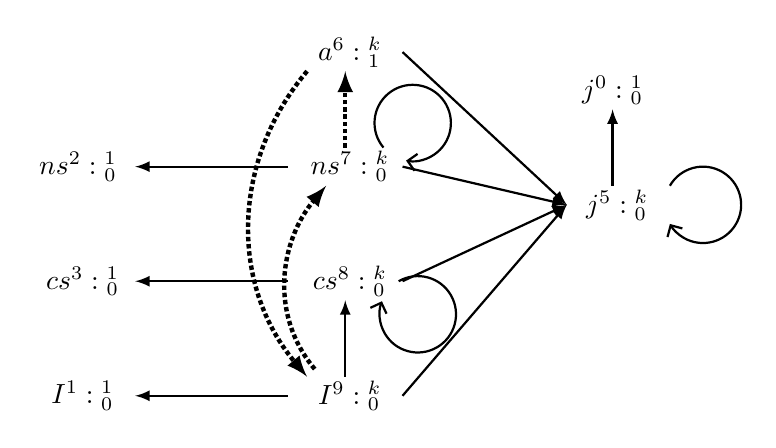
\begin{tikzpicture}[scale=\textwidth/25cm,samples=200]
% Variables Initialization
\draw[] (-7, 1) circle (0pt) node{{ $I^1: {}^1_{0}$}};
\draw[] (-7, 7) circle (0pt) node{{$ns^2: {}^{1}_{0}$}};
\draw[] (-7, 4) circle (0pt) node{{ $cs^3: {}^{1}_{0}$}};
% Variables Inside the Loop
     \draw[] (0, 10) circle (0pt) node{{ $a^6: {}^{k}_{1}$}};
     \draw[] (0, 7) circle (0pt) node{{ $ns^7: {}^{k}_{0}$}};
     \draw[] (0, 4) circle (0pt) node{{ $cs^8: {}^{k}_{0}$}};
     \draw[] (0, 1) circle (0pt) node{{ $I^9: {}^{k}_{0}$}};
     % Counter Variables
     \draw[] (7, 9) circle (0pt) node {{$j^0: {}^{1}_{0}$}};
     \draw[] (7, 6) circle (0pt) node {{ $j^5: {}^{k}_{0}$}};
     %
     % Value Dependency Edges:
     \draw[ thick, -latex,] (0, 1.5)  -- (0, 3.5) ;
     \draw[ ultra thick, -latex, densely dotted,] (0, 7.5)  -- (0, 9.5) ;
     \draw[ thick, -Straight Barb] (1.4, 4) arc (120:-200:1);
     \draw[ thick, -Straight Barb] (8.5, 6.5) arc (150:-150:1);
     \draw[ thick, -Straight Barb] (1, 7.5) arc (220:-100:1);
     \draw[ thick, -latex] (7, 6.5)  -- (7, 8.5) ;
     % Value Dependency Edges on Initial Values:
     \draw[ thick, -latex,] (-1.5, 1)  -- (-5.5, 1) ;
     \draw[ thick, -latex,] (-1.5, 4)  -- (-5.5, 4) ;
     \draw[ thick, -latex,] (-1.5, 7)  -- (-5.5, 7) ;
     %
     \draw[ ultra thick, -latex, densely dotted,] (-1, 9.5)  to  [out=-130,in=130]  (-1, 1.5);
     \draw[ ultra thick, -latex, densely dotted,] (-0.8, 1.7)  to  [out=-230,in=230]  (-0.5, 6.5);
     % Control Dependency
    %  \draw[ thick,-latex] (1.5, 7)  -- (4, 9) ;
    %  \draw[ thick,-latex] (1.5, 4)  -- (4, 9) ;
     \draw[ thick,-latex] (1.5, 7)  -- (5.8, 6) ;
     \draw[ thick,-latex] (1.5, 4)  -- (5.8, 6) ;
     \draw[ thick,-latex] (1.5, 1)  -- (5.8, 6) ;
     \draw[ thick,-latex] (1.5, 10)  -- (5.8, 6) ;
     \end{tikzpicture}
     \caption{}
        \end{centering}
        \end{subfigure}
    \vspace{-0.4cm}
    \caption{(a) The simplified multiple rounds example (b) The program-based dependency graph from $\THESYSTEM$}
    \vspace{-0.5cm}
    \label{fig:multi_graphs}
\end{figure}
%
\end{example}

My static analysis provides an upper bound on the adaptivity for this example as follows.
{\THESYSTEM} constructs a program-based dependency graph, for my example we show this graph in 
Figure~\ref{fig:twoRounds_example}(c).
The edges of this graph are built by considering both control flow and data flow between assigned variables (the algorithm is presented in Section~\ref{subsubsec:static-datadep}). 
The weight of every vertex is estimated by using a reachability-bound estimation algorithm 
(presented in Section~\ref{subsubsec:static-reachability}), which can be symbolic and provide a sound upper bound on the weight of the corresponding vertex in the execution-based dependency graph. 
For instance, the weight $k$ of the vertex $x^{3}$ in Figure~\ref{fig:twoRounds_example}(c) is a sound upper bound on the weight $w_k$ of vertex $x^{3}$ in Figure~\ref{fig:twoRounds_example}(b), with the same starting trace. 
The soundness of this step is proved in Theorem~\ref{thm:addweight_soundness}.

$\THESYSTEM$ search a walk on this graph which over-approximate the adaptivity of the program (this is done by an algorithm
$\pathsearch$ presented in  Section~\ref{subsubsec:static-adapt}). 
%  finds a finite walk on this graph.
% This finite walk traverses the maximum times of query variables, 
% and the visiting time of every vertex on this walk is restricted by its weight.
% The maximum number of vertices visited on this walk which correspond to query variables, is the final estimated adaptivity upper bound, for the program.
For instance, in Figure~\ref{fig:twoRounds_example}(c), $\pathsearch$ first finds a path $l^6:{}^1_1 \to a^5: {}^k_1 \to x^3: {}^k_1$, and then approximate a walk with this path.
Every vertex on this walk is visited once, and the number of vertices with query annotation $1$ traversed in this path is $2$, which is the upper bound we expect.
It is worth to note here that even though the node $x^3$ has weight depending on $k$, 
it is only visited once, similarly for $l^6$, hence the overall upper bound on the adaptivity is 2, as we expect.
%
% \subsection{Implementation}
% \label{subsec:static-implementation}

% \cleardoublepage

\section{Status and Plan}

\subsection{Status}


\subsection{Plan}
\begin{itemize}
\item August 15, 2022: Finish accurate execution-based dependency depth analysis and implementation
\item September 01, 2022: Finish Path Sensitive Reachability Bound Algorithm Formalization and Implementation
\item September 30, 2022: Finish re-writing the adaptivity analysis for adaptive data analysis program paper towards Journal
\item October 15, 2022: Finish Path Sensitive Reachability Bound paper writing towards PLDI
\item November 10, 2022 : Submit to PLDI 2023
\item November 20, 2022 : Finish thesis
\item December 05, 2022 : Defend
\end{itemize}


\bibliographystyle{plain}
\bibliography{main.bib}

\end{document}
